% Options for packages loaded elsewhere
\PassOptionsToPackage{unicode}{hyperref}
\PassOptionsToPackage{hyphens}{url}
%
\documentclass[
  11pt,
  openright,twoside]{book}
\usepackage{amsmath,amssymb}
\usepackage{lmodern}
\usepackage{iftex}
\ifPDFTeX
  \usepackage[T1]{fontenc}
  \usepackage[utf8]{inputenc}
  \usepackage{textcomp} % provide euro and other symbols
\else % if luatex or xetex
  \usepackage{unicode-math}
  \defaultfontfeatures{Scale=MatchLowercase}
  \defaultfontfeatures[\rmfamily]{Ligatures=TeX,Scale=1}
\fi
% Use upquote if available, for straight quotes in verbatim environments
\IfFileExists{upquote.sty}{\usepackage{upquote}}{}
\IfFileExists{microtype.sty}{% use microtype if available
  \usepackage[]{microtype}
  \UseMicrotypeSet[protrusion]{basicmath} % disable protrusion for tt fonts
}{}
\makeatletter
\@ifundefined{KOMAClassName}{% if non-KOMA class
  \IfFileExists{parskip.sty}{%
    \usepackage{parskip}
  }{% else
    \setlength{\parindent}{0pt}
    \setlength{\parskip}{6pt plus 2pt minus 1pt}}
}{% if KOMA class
  \KOMAoptions{parskip=half}}
\makeatother
\usepackage{xcolor}
\usepackage[textwidth=6in,textheight=8in]{geometry}
\usepackage{color}
\usepackage{fancyvrb}
\newcommand{\VerbBar}{|}
\newcommand{\VERB}{\Verb[commandchars=\\\{\}]}
\DefineVerbatimEnvironment{Highlighting}{Verbatim}{commandchars=\\\{\}}
% Add ',fontsize=\small' for more characters per line
\usepackage{framed}
\definecolor{shadecolor}{RGB}{248,248,248}
\newenvironment{Shaded}{\begin{snugshade}}{\end{snugshade}}
\newcommand{\AlertTok}[1]{\textcolor[rgb]{0.94,0.16,0.16}{#1}}
\newcommand{\AnnotationTok}[1]{\textcolor[rgb]{0.56,0.35,0.01}{\textbf{\textit{#1}}}}
\newcommand{\AttributeTok}[1]{\textcolor[rgb]{0.77,0.63,0.00}{#1}}
\newcommand{\BaseNTok}[1]{\textcolor[rgb]{0.00,0.00,0.81}{#1}}
\newcommand{\BuiltInTok}[1]{#1}
\newcommand{\CharTok}[1]{\textcolor[rgb]{0.31,0.60,0.02}{#1}}
\newcommand{\CommentTok}[1]{\textcolor[rgb]{0.56,0.35,0.01}{\textit{#1}}}
\newcommand{\CommentVarTok}[1]{\textcolor[rgb]{0.56,0.35,0.01}{\textbf{\textit{#1}}}}
\newcommand{\ConstantTok}[1]{\textcolor[rgb]{0.00,0.00,0.00}{#1}}
\newcommand{\ControlFlowTok}[1]{\textcolor[rgb]{0.13,0.29,0.53}{\textbf{#1}}}
\newcommand{\DataTypeTok}[1]{\textcolor[rgb]{0.13,0.29,0.53}{#1}}
\newcommand{\DecValTok}[1]{\textcolor[rgb]{0.00,0.00,0.81}{#1}}
\newcommand{\DocumentationTok}[1]{\textcolor[rgb]{0.56,0.35,0.01}{\textbf{\textit{#1}}}}
\newcommand{\ErrorTok}[1]{\textcolor[rgb]{0.64,0.00,0.00}{\textbf{#1}}}
\newcommand{\ExtensionTok}[1]{#1}
\newcommand{\FloatTok}[1]{\textcolor[rgb]{0.00,0.00,0.81}{#1}}
\newcommand{\FunctionTok}[1]{\textcolor[rgb]{0.00,0.00,0.00}{#1}}
\newcommand{\ImportTok}[1]{#1}
\newcommand{\InformationTok}[1]{\textcolor[rgb]{0.56,0.35,0.01}{\textbf{\textit{#1}}}}
\newcommand{\KeywordTok}[1]{\textcolor[rgb]{0.13,0.29,0.53}{\textbf{#1}}}
\newcommand{\NormalTok}[1]{#1}
\newcommand{\OperatorTok}[1]{\textcolor[rgb]{0.81,0.36,0.00}{\textbf{#1}}}
\newcommand{\OtherTok}[1]{\textcolor[rgb]{0.56,0.35,0.01}{#1}}
\newcommand{\PreprocessorTok}[1]{\textcolor[rgb]{0.56,0.35,0.01}{\textit{#1}}}
\newcommand{\RegionMarkerTok}[1]{#1}
\newcommand{\SpecialCharTok}[1]{\textcolor[rgb]{0.00,0.00,0.00}{#1}}
\newcommand{\SpecialStringTok}[1]{\textcolor[rgb]{0.31,0.60,0.02}{#1}}
\newcommand{\StringTok}[1]{\textcolor[rgb]{0.31,0.60,0.02}{#1}}
\newcommand{\VariableTok}[1]{\textcolor[rgb]{0.00,0.00,0.00}{#1}}
\newcommand{\VerbatimStringTok}[1]{\textcolor[rgb]{0.31,0.60,0.02}{#1}}
\newcommand{\WarningTok}[1]{\textcolor[rgb]{0.56,0.35,0.01}{\textbf{\textit{#1}}}}
\usepackage{longtable,booktabs,array}
\usepackage{calc} % for calculating minipage widths
% Correct order of tables after \paragraph or \subparagraph
\usepackage{etoolbox}
\makeatletter
\patchcmd\longtable{\par}{\if@noskipsec\mbox{}\fi\par}{}{}
\makeatother
% Allow footnotes in longtable head/foot
\IfFileExists{footnotehyper.sty}{\usepackage{footnotehyper}}{\usepackage{footnote}}
\makesavenoteenv{longtable}
\usepackage{graphicx}
\makeatletter
\def\maxwidth{\ifdim\Gin@nat@width>\linewidth\linewidth\else\Gin@nat@width\fi}
\def\maxheight{\ifdim\Gin@nat@height>\textheight\textheight\else\Gin@nat@height\fi}
\makeatother
% Scale images if necessary, so that they will not overflow the page
% margins by default, and it is still possible to overwrite the defaults
% using explicit options in \includegraphics[width, height, ...]{}
\setkeys{Gin}{width=\maxwidth,height=\maxheight,keepaspectratio}
% Set default figure placement to htbp
\makeatletter
\def\fps@figure{htbp}
\makeatother
\setlength{\emergencystretch}{3em} % prevent overfull lines
\providecommand{\tightlist}{%
  \setlength{\itemsep}{0pt}\setlength{\parskip}{0pt}}
\setcounter{secnumdepth}{5}
\usepackage{amsmath,amssymb,unicode-math,tikz,xcolor,sectsty,regexpatch,letltxmacro,makeidx}
%% elements of style
\definecolor{WildStrawberry}{rgb}{1,.26,.64}
\usepackage{fancyhdr}
\makeatletter
\renewcommand{\@chapapp}{Section}
\makeatother
\pagestyle{fancy}
\renewcommand{\chaptermark}[1]{\markboth{#1}{}}
\renewcommand{\sectionmark}[1]{\markright{#1}}
\fancyhead{} % clear all header fields
\fancyfoot{} % clear all footer fields
\fancyfoot[LE]{\thepage\ |\ \nouppercase{\leftmark}}
\fancyfoot[RO]{\nouppercase{\rightmark}\ |\ \thepage}
\renewcommand{\headrulewidth}{0pt}
\renewcommand{\footrulewidth}{0.4pt}
\renewcommand{\footrule}{\hbox to\headwidth{%
    \color{WildStrawberry}\leaders\hrule height \footrulewidth\hfill}}
\fancypagestyle{plain}{%
  \fancyhead{} % clear all header fields
  \fancyfoot{} % clear all footer fields
  \fancyfoot[LE]{\thepage\ |\ \nouppercase{\leftmark}}
  \fancyfoot[RO]{\nouppercase{\rightmark}\ |\ \thepage}
  \renewcommand{\headrulewidth}{0pt}
  \renewcommand{\footrulewidth}{0.4pt}
  \renewcommand{\footrule}{\hbox to\headwidth{%
      \color{WildStrawberry}\leaders\hrule height \footrulewidth\hfill}}
}
%%
\makeatletter
\newcommand{\setchapterrulecolor}[1]{\colorlet{secrulecolor}{#1}}
\setchapterrulecolor{WildStrawberry}
\xpatchcmd*{\SS@normsectionrule}% <cmd>
  {\rule}% <search>
  {\color{secrulecolor}\rule}% <replace>
  {}{}% <success><failure>
% \newcommand{\setsectionrulecolor}[1]{\colorlet{secrulecolor}{#1}}
% \setsectionrulecolor{WildStrawberry}
% \xpatchcmd*{\SS@normsectionrule}% <cmd>
%   {\rule}% <search>
%   {\color{secrulecolor}\rule}% <replace>
%   {}{}% <success><failure>
\makeatother
\chapterfont{\sectionrule{0pt}{0pt}{-5pt}{0.8pt}}
% \sectionfont{\sectionrule{0pt}{0pt}{-5pt}{0.8pt}}


%% newcommands

\DeclareMathOperator{\Dirac}{Dirac}
\DeclareMathOperator{\expit}{expit}
\DeclareMathOperator{\logit}{logit}
\DeclareMathOperator{\Rem}{Rem}
\DeclareMathOperator{\Var}{Var}

%% %% exercize symbol

\newsavebox\gearbox
\newcommand{\gearmacro}[5]{%
  % #1 number of teeths
  % #2 radius intern
  % #3 radius extern
  % #4 angle from start to end of the first arc
  % #5 angle to decale the second arc from the first 
  \foreach \i in {1,...,#1} {%
    [rotate=(\i-1)*360/#1]  (0:#2)  arc (0:#4:#2) {[rounded corners=1.5pt]
      -- (#4+#5:#3)  arc (#4+#5:360/#1-#5:#3)} --  (360/#1:#2)
  }}  
\newcommand{\makegear}{\begin{tikzpicture}
    \fill[gray] (0,0) circle (2cm);
    \draw[thick,rotate=12,fill=gray] \gearmacro{8}{2}{2.4}{20}{2};
    \draw[thick,fill=white] (0cm,0cm) circle(1.35cm);
  \end{tikzpicture}}
\sbox\gearbox{\resizebox{!}{1em}{\makegear}}
\newcommand{\gear}{\usebox{\gearbox}\;}

%% %% danger symbol

\DeclareFontFamily{U}{stixbbit}{}
\DeclareFontShape{U}{stixbbit}{m}{it}{<-> stix-mathbbit}{}
\DeclareRobustCommand{\stixdanger}{%
  {\usefont{U}{stixbbit}{m}{it}\symbol{"F6}}%
}


\newcommand{\bbO}{\mathbb{O}}
\newcommand{\bbD}{\mathbb{D}}
\newcommand{\bbP}{\mathbb{P}}
\newcommand{\bbR}{\mathbb{R}}
\newcommand{\Algo}{\widehat{\mathcal{A}}}
\newcommand{\Algora}{\widetilde{\mathcal{A}}}
\newcommand{\defq}{\doteq}
\newcommand{\calF}{\mathcal{F}}
\newcommand{\calM}{\mathcal{M}}
\newcommand{\calP}{\mathcal{P}}
\newcommand{\calO}{\mathcal{O}}
\newcommand{\calQ}{\mathcal{Q}}
\newcommand{\Exp}{\textrm{E}}
\newcommand{\IC}{\textrm{IC}}
\newcommand{\Gbar}{\bar{G}}
\newcommand{\one}{\textbf{1}}
\newcommand{\psinos}{\psi_{n}^{\textrm{os}}}
\renewcommand{\Pr}{\textrm{Pr}}
\newcommand{\Phat}{P^{\circ}}
\newcommand{\Psihat}{\widehat{\Psi}}
\newcommand{\Qbar}{\bar{Q}}
\newcommand{\tcg}[1]{\textcolor{olive}{#1}}

\allowdisplaybreaks

\makeindex

%%% Local Variables:
%%% mode: latex
%%% TeX-master: t
%%% End:
\ifLuaTeX
  \usepackage{selnolig}  % disable illegal ligatures
\fi
\usepackage[]{natbib}
\bibliographystyle{plainnat}
\IfFileExists{bookmark.sty}{\usepackage{bookmark}}{\usepackage{hyperref}}
\IfFileExists{xurl.sty}{\usepackage{xurl}}{} % add URL line breaks if available
\urlstyle{same} % disable monospaced font for URLs
\hypersetup{
  pdftitle={A Ride in Targeted Learning Territory},
  pdfauthor={David Benkeser (Emory University); Antoine Chambaz (Université Paris Cité)},
  hidelinks,
  pdfcreator={LaTeX via pandoc}}

\title{A Ride in Targeted Learning Territory}
\author{David Benkeser (Emory University) \and Antoine Chambaz (Université Paris Cité)}
\date{2022-10-20}

\usepackage{amsthm}
\newtheorem{theorem}{Theorem}[chapter]
\newtheorem{lemma}{Lemma}[chapter]
\newtheorem{corollary}{Corollary}[chapter]
\newtheorem{proposition}{Proposition}[chapter]
\newtheorem{conjecture}{Conjecture}[chapter]
\theoremstyle{definition}
\newtheorem{definition}{Definition}[chapter]
\theoremstyle{definition}
\newtheorem{example}{Example}[chapter]
\theoremstyle{definition}
\newtheorem{exercise}{Exercise}[chapter]
\theoremstyle{definition}
\newtheorem{hypothesis}{Hypothesis}[chapter]
\theoremstyle{remark}
\newtheorem*{remark}{Remark}
\newtheorem*{solution}{Solution}
\begin{document}
\maketitle

\begin{titlepage}
  \centering
  \vspace*{3cm}
  \begin{Huge}
    {\color{WildStrawberry}{\hrule}}
    \vspace{1cm}
    A Ride in Targeted Learning Territory
    \vspace{1cm}
    {\color{WildStrawberry}{\hrule}}
  \end{Huge}
  \vspace*{1cm}  
  \begin{large}
    David Benkeser (Emory Univeristy)\\~\\
    Antoine Chambaz (Universit\'e Paris Cité)\\~\\
    \today\par
  \end{large}
  \vspace*{1cm}
  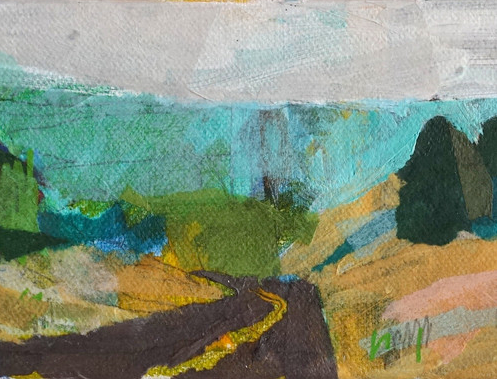
\includegraphics{cover.jpg}\\
  \textit{Long Mendocino Drive}\\
  (detail, Liana Steinmetz)
\end{titlepage}



%%% Local Variables:
%%% mode: latex
%%% TeX-master: t
%%% End:

{
\setcounter{tocdepth}{1}
\tableofcontents
}
\hypertarget{welcome}{%
\chapter*{Welcome}\label{welcome}}
\addcontentsline{toc}{chapter}{Welcome}

This is either the website or the text called \textbf{``A Ride in Targeted Learning
Territory''}. In the former case, the text can be dowloaded by clicking on the
dedicated button in the top part of the webpage. In the latter case, the
website can be browsed at
\url{https://achambaz.github.io/tlride/}.

\begin{center}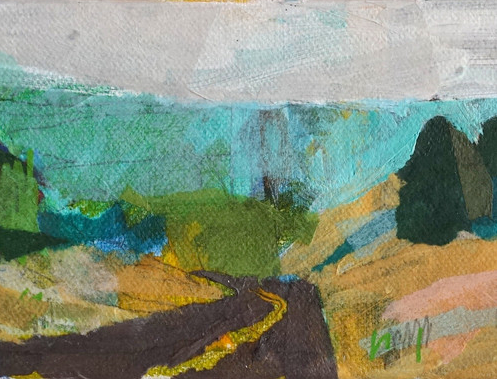
\includegraphics[width=0.7\linewidth]{cover} \end{center}

\begin{center}
Long Mendocino Drive (detail,
\href{https://www.lianasteinmetz.com/}{Liana Steinmetz})
\end{center}

\textbf{Organization}

The text takes the form of a series of brief sections. The main sections
combine theoretical and computational developments. The code is written in the
programming language \href{https://www.r-project.org}{\texttt{R}} \citep{R}. \texttt{R} is widely
used among statisticians and data scientists to develop statistical software
and data analysis.

Regularly, a section is inserted that proposes exercises. Each such section
is indicated by the {⚙} \gear symbol. The
symbol {☡} \stixdanger{} also indicates
those sections of which the content is more involved.

\textbf{Overview}

After a short introduction, we present the reproducible experiment that will
play a central role throughout the text. Then, we introduce the main parameter
of interest. We comment upon some of its properties that are useful from a
statistical perspective. This paves the way to the presentation of several
estimators that are increasingly more powerful statistically. The discussion
takes us into \emph{targeted learning territory}.

\textbf{Audience}

The text might be of interest to students in statistics and machine
learning. It might also serve as a gentle introduction to targeted learning in
both its theoretical and computational aspects before delving deeper into the
literature \citep{TMLEbook11}, \citep{TMLEbook18}.

The text was presented at the \href{https://www.sfds.asso.fr/fr/group/activites_et_parrainages/608-journees_detude_en_statistique/}{Journées d'Étude en Statistique
2018}
held in Fréjus (France) in October 2018 and at the \href{https://ehermellin.github.io/conf_sfds/index.html}{First Summer School in
Statistics and Data Science for Young Researchers from French-speaking
Africa} held at \href{https://aims-senegal.org/}{AIMS
Senegal} (MBour, Senegal) in July 2019. The text
and a shorter version (in French) will be published soon \citep{BC20}, \citep{BCJES20}.

\textbf{Technical details}

The text is written in \href{https://rmarkdown.rstudio.com}{\texttt{RMarkdown}}
with \href{https://bookdown.org}{\texttt{bookdown}}. Assuming that
the \href{https://yihui.name/knitr/}{\texttt{knitr}} package is installed, you can
retrieve all the \texttt{R} code by cloning this \href{https://github.com/achambaz/tlride}{\texttt{github}
repository} then running

\begin{Shaded}
\begin{Highlighting}[]
\NormalTok{knitr}\SpecialCharTok{::}\FunctionTok{purl}\NormalTok{(}\StringTok{"abcd.Rmd"}\NormalTok{)}
\end{Highlighting}
\end{Shaded}

\hypertarget{part-on-the-road}{%
\part{On the road}\label{part-on-the-road}}

\hypertarget{a-ride}{%
\chapter{A ride}\label{a-ride}}

\hypertarget{introduction}{%
\section{Introduction}\label{introduction}}

Our ambition is to present a gentle introduction to the field of targeted
learning. As an example, we consider statistical inference on a simple causal
quantity that is ubiquitous in the causal literature. We use this exemplar
parameter to introduce key concepts that can be applied to more complicated
problems. The introduction weaves together two main threads, one theoretical
and the other computational.

\hypertarget{causal-story}{%
\subsection{A causal story}\label{causal-story}}

We focus on a causal story where a random reward (a real number between 0 and
1) is given based on an action undertaken (one among two) and the random
context where the action is performed (summarized by a real number between 0
and 1). The causal quantity of interest is the average difference of the two
counterfactual rewards. This is a story as old as time. Should we take the red
pill or the blue pill? Should we show our customers advertisement A or
advertisement B? Should we require individuals to undergo cancer screening? At
their core, each of these questions is asking what action should be taken to
maximize a ``reward.''

We will build several estimators and discuss their respective merits,
theoretically and computationally. The construction of the most involved
estimator will unfold in \emph{targeted learning territory}, at the frontier of
machine learning and semiparametrics, the statistical theory of inference
based on semiparametric models.

\hypertarget{tlrider-package}{%
\subsection{\texorpdfstring{The \texttt{tlrider} package}{The tlrider package}}\label{tlrider-package}}

The computational illustrations will be developed based on the companion
package \texttt{tlrider}. The package can be installed by
running the following code:

\begin{Shaded}
\begin{Highlighting}[]
\NormalTok{devtools}\SpecialCharTok{::}\FunctionTok{install\_github}\NormalTok{(}\StringTok{"achambaz/tlride/tlrider"}\NormalTok{)}
\end{Highlighting}
\end{Shaded}

The version used in this document is 1.1.1.

Additional packages are also required, including \texttt{tidyverse} \citep{r4ds}, \texttt{caret}
\citep{caret} and \texttt{ggdag} \citep{ggdag}. Assuming that these are installed too, we can
run the next chunk of code:

\begin{Shaded}
\begin{Highlighting}[]
\FunctionTok{library}\NormalTok{(tidyverse)}
\FunctionTok{library}\NormalTok{(caret)}
\FunctionTok{library}\NormalTok{(ggdag)}
\FunctionTok{library}\NormalTok{(tlrider)}
\end{Highlighting}
\end{Shaded}

\hypertarget{discuss}{%
\subsection{What we will discuss}\label{discuss}}

To begin, we discuss the nature of the parameter of interest, viewing it as
the value of a statistical mapping evaluated at the law of the data (Section
\ref{parameter}), with an emphasis on the smoothness and double-robustness
properties inherited from the mapping (Sections \ref{smooth} and
\ref{double-robustness}). We then turn to the estimation of the parameter of
interest. We first introduce and comment upon a simple inference strategy
assuming provisionally that a relevant feature of the law of the data is known
to us (Section \ref{simple-strategy}). Second, we present the notion of
nuisance parameters and adopt an algorithmic stance on their estimation
(Section \ref{nuisance}). Third, we introduce and comment upon two ``naive''
inference strategies (Section \ref{naive-estimators}), the one-step
correction procedure (Section \ref{one-step}) and, finally, the targeted
minimum loss estimation procedure tailored to the inference of the parameter
of main interest. In the appendix, we collect our notation (Section
\ref{notation}), and present some results that are used in the main text and
their proofs (Sections \ref{proofs} and \ref{more-proofs}).

\hypertarget{simulation-study}{%
\section{A simulation study}\label{simulation-study}}

\hypertarget{reproducible-experiment}{%
\subsection{Reproducible experiment as a law}\label{reproducible-experiment}}

We are interested in a reproducible experiment. Every time this experiment is
run, it generates an observation that we call \(O\). We view \(O\) as a random
variable drawn from \emph{the law of the experiment} that we denote by \(P_{0}\).

We view \(P_{0}\) as an element of \emph{the model} \(\calM\). The model is a
collection of laws. In particular, the model contains all laws that we think
may plausibly describe the law of the experiment. Thus, the choice of model
is based on our scientific knowledge of the experiment. The more we know about
the experiment, the smaller is \(\calM\). In all our examples, we use large
models that reflect a lack of knowledge about many aspects of the experiment.

\hypertarget{synthetic-experiment}{%
\subsection{A synthetic reproducible experiment}\label{synthetic-experiment}}

Instead of considering a real-life reproducible experiment, we focus for
pedagogical purposes on a \emph{synthetic} reproducible experiment. Thus we can
from now on take on two different roles: that of an \emph{oracle} knowing
completely the nature of the experiment, and that of a \emph{statistician} eager to
know more about the experiment by observing some of its outputs.

Let us run the example built into the \texttt{tlrider} package:

\begin{Shaded}
\begin{Highlighting}[]
\FunctionTok{example}\NormalTok{(tlrider)}
\end{Highlighting}
\end{Shaded}

A few objects have been defined:

\begin{Shaded}
\begin{Highlighting}[]
\FunctionTok{ls}\NormalTok{()}
\CommentTok{\#\textgreater{} [1] "another\_experiment" "experiment"         "expit"             }
\CommentTok{\#\textgreater{} [4] "filter"             "logit"              "sigma0"}
\end{Highlighting}
\end{Shaded}

The function \texttt{expit} implements the link function \(\expit : \bbR \to ]0,1[\) given
by \(\expit(x) \defq (1 + e^{-x})^{-1}\). The function \texttt{logit} implements its
inverse function \(\logit : ]0,1[ \to \bbR\) given by \(\logit(p) \defq \log [p/(1-p)]\).

Let us take a look at \texttt{experiment}:

\begin{Shaded}
\begin{Highlighting}[]
\NormalTok{experiment}
\CommentTok{\#\textgreater{} A law for (W,A,Y) in [0,1] x \{0,1\} x [0,1].}
\CommentTok{\#\textgreater{} }
\CommentTok{\#\textgreater{} If the law is fully characterized, you can use method}
\CommentTok{\#\textgreater{} \textquotesingle{}sample\_from\textquotesingle{} to sample from it.}
\CommentTok{\#\textgreater{} }
\CommentTok{\#\textgreater{} If you built the law, or if you are an \_oracle\_, you can also}
\CommentTok{\#\textgreater{} use methods \textquotesingle{}reveal\textquotesingle{} to reveal its relevant features (QW, Gbar,}
\CommentTok{\#\textgreater{} Qbar, qY {-}{-} see \textquotesingle{}?reveal\textquotesingle{}), and \textquotesingle{}alter\textquotesingle{} to change some of them.}
\CommentTok{\#\textgreater{} }
\CommentTok{\#\textgreater{} If all its relevant features are characterized, you can use}
\CommentTok{\#\textgreater{} methods \textquotesingle{}evaluate\_psi\textquotesingle{} to obtain the value of \textquotesingle{}Psi\textquotesingle{} at this law}
\CommentTok{\#\textgreater{} (see \textquotesingle{}?evaluate\_psi\textquotesingle{}) and \textquotesingle{}evaluate\_eic\textquotesingle{} to obtain the efficient}
\CommentTok{\#\textgreater{} influence curve of \textquotesingle{}Psi\textquotesingle{} at this law (see \textquotesingle{}?evaluate\_eic\textquotesingle{}).}
\end{Highlighting}
\end{Shaded}

The law \(P_{0}\) of the synthetic experiment \texttt{experiment} built by us generates
a generic observation \(O\) that decomposes as \begin{equation*} O \defq (W, A,
Y) \in [0,1] \times \{0,1\} \times [0,1].  \end{equation*} We interpret \(W\) as
a real valued summary measure of a random context where an action \(A\) chosen
among two is undertaken, leading to a real valued reward \(Y\).

We can sample from the experiment (simply run \texttt{?sample\_from} to see the man
page of method \texttt{sample\_from}). The next chunk of code runs the experiment five
times, independently:

\begin{Shaded}
\begin{Highlighting}[]
\NormalTok{(five\_obs }\OtherTok{\textless{}{-}} \FunctionTok{sample\_from}\NormalTok{(experiment, }\AttributeTok{n =} \DecValTok{5}\NormalTok{))}
\CommentTok{\#\textgreater{}          W A     Y}
\CommentTok{\#\textgreater{} [1,] 0.393 1 0.789}
\CommentTok{\#\textgreater{} [2,] 0.399 1 0.782}
\CommentTok{\#\textgreater{} [3,] 0.373 1 0.942}
\CommentTok{\#\textgreater{} [4,] 0.371 1 0.838}
\CommentTok{\#\textgreater{} [5,] 0.372 1 0.779}
\end{Highlighting}
\end{Shaded}

\hypertarget{revealing-experiment}{%
\subsection{\texorpdfstring{Revealing \texttt{experiment}}{Revealing experiment}}\label{revealing-experiment}}

Acting as oracles, we can peek into \texttt{experiment} and \emph{reveal} a selection of
relevant features (simply run \texttt{?reveal} to see the man page of method
\texttt{reveal}). Made by us, the selection exhibits features that will play an
important role in the text.

\begin{Shaded}
\begin{Highlighting}[]
\NormalTok{relevant\_features }\OtherTok{\textless{}{-}} \FunctionTok{reveal}\NormalTok{(experiment)}
\FunctionTok{names}\NormalTok{(relevant\_features)}
\CommentTok{\#\textgreater{} [1] "QW"          "Gbar"        "Qbar"        "qY"          "sample\_from"}
\end{Highlighting}
\end{Shaded}

We have an oracular knowledge of \texttt{experiment} and can thus comment upon the
features of \(P_{0}\) revealed in \texttt{relevant\_features}.

\hypertarget{qw}{%
\subsubsection*{\texorpdfstring{\texttt{QW}}{QW}}\label{qw}}
\addcontentsline{toc}{subsubsection}{\texttt{QW}}

The \texttt{QW} feature describes the marginal law of \(W\), that we call \(Q_{0,W}\).\footnote{A
  summary of the notation used throughout the text is presented
  \protect\hyperlink{notation}{there}, in Appendix \ref{notation}.}

\begin{Shaded}
\begin{Highlighting}[]
\NormalTok{relevant\_features}\SpecialCharTok{$}\NormalTok{QW}
\CommentTok{\#\textgreater{} function(W,}
\CommentTok{\#\textgreater{}                     mixture\_weights = c(1/10, 9/10, 0),}
\CommentTok{\#\textgreater{}                     mins = c(0, 11/30, 0),}
\CommentTok{\#\textgreater{}                     maxs = c(1, 14/30, 1)) \{}
\CommentTok{\#\textgreater{}         out \textless{}{-} sapply(1:length(mixture\_weights),}
\CommentTok{\#\textgreater{}                       function(ii)\{}
\CommentTok{\#\textgreater{}                         mixture\_weights[ii] *}
\CommentTok{\#\textgreater{}                           stats::dunif(W,}
\CommentTok{\#\textgreater{}                                        min = mins[ii],}
\CommentTok{\#\textgreater{}                                        max = maxs[ii])}
\CommentTok{\#\textgreater{}                       \})}
\CommentTok{\#\textgreater{}         return(rowSums(out))}
\CommentTok{\#\textgreater{}       \}}
\CommentTok{\#\textgreater{} \textless{}environment: 0x55d8a4b54758\textgreater{}}
\end{Highlighting}
\end{Shaded}

It appears that \(Q_{0,W}\) is a mixture of the uniform laws over \([0,1]\)
(weight \(1/10\)) and \([11/30,14/30]\) (weight \(9/10\)).\footnote{We fine-tuned the
  marginal law \(Q_{0,W}\) of \(W\) to make it easier later on to drive home
  important messages.}

\hypertarget{gbar}{%
\subsubsection*{\texorpdfstring{\texttt{Gbar}}{Gbar}}\label{gbar}}
\addcontentsline{toc}{subsubsection}{\texttt{Gbar}}

The \texttt{Gbar} feature describes the conditional probability of action \(A = 1\)
given \(W\). For each \(a \in \{0,1\}\), we denote \begin{align*}  \Gbar_0(W)
&\defq \Pr_{P_0}(A  = 1 |  W), \\\ell\Gbar_0(a,W)  &\defq \Pr_{P_0}(A =  a |
W).\end{align*} Obviously, \begin{equation*}\ell\Gbar_{0}(A,W)    =
A\Gbar_{0}(W) + (1-A) (1-\Gbar_{0}(W)).\end{equation*}

\begin{Shaded}
\begin{Highlighting}[]
\NormalTok{relevant\_features}\SpecialCharTok{$}\NormalTok{Gbar}
\CommentTok{\#\textgreater{} function(W) \{}
\CommentTok{\#\textgreater{}         expit(1 + 2 * W {-} 4 * sqrt(abs((W {-} 5/12))))}
\CommentTok{\#\textgreater{}       \}}
\CommentTok{\#\textgreater{} \textless{}environment: 0x55d8a4b54758\textgreater{}}
\end{Highlighting}
\end{Shaded}

Note how real numbers of the form \(1 + 2W - 4 * \sqrt{|W - 5/12|})\) are mapped
into the interval \([0,1]\) by the \(\expit\) link function. We refer the reader
to Figure \ref{fig:estimate-Gbar-three} for a visualization of \(\Gbar_{0}\).

\hypertarget{qy}{%
\subsubsection*{\texorpdfstring{\texttt{qY}}{qY}}\label{qy}}
\addcontentsline{toc}{subsubsection}{\texttt{qY}}

The \texttt{qY} feature describes the conditional density of \(Y\) given \(A\) and \(W\).
For each \(y\in ]0,1[\), we denote by \(q_{0,Y}(y, A, W)\) the conditional density
evaluated at \(y\) of \(Y\) given \(A\) and \(W\).

\begin{Shaded}
\begin{Highlighting}[]
\NormalTok{relevant\_features}\SpecialCharTok{$}\NormalTok{qY}
\CommentTok{\#\textgreater{} function(obs, Qbar, shape10 = 2, shape11 = 3)\{}
\CommentTok{\#\textgreater{}         A \textless{}{-} obs[, "A"]}
\CommentTok{\#\textgreater{}         AW \textless{}{-} obs[, c("A", "W")]}
\CommentTok{\#\textgreater{}         QAW \textless{}{-} Qbar(AW)}
\CommentTok{\#\textgreater{}         shape1 \textless{}{-} ifelse(A == 0, shape10, shape11)}
\CommentTok{\#\textgreater{}         stats::dbeta(Y,}
\CommentTok{\#\textgreater{}                      shape1 = shape1,}
\CommentTok{\#\textgreater{}                      shape2 = shape1 * (1 {-} QAW) / QAW)}
\CommentTok{\#\textgreater{}       \}}
\CommentTok{\#\textgreater{} \textless{}environment: 0x55d8a4b54758\textgreater{}}
\end{Highlighting}
\end{Shaded}

It appears that the conditional law of \(Y\) given \(A\) and \(W\) is the Beta law
with conditional mean and variance characterized by the \texttt{Qbar} feature of
\texttt{experiment} (see below) and the \texttt{shape10} and \texttt{shape11} parameters.

\hypertarget{qbar}{%
\subsubsection*{\texorpdfstring{\texttt{Qbar}}{Qbar}}\label{qbar}}
\addcontentsline{toc}{subsubsection}{\texttt{Qbar}}

As for the \texttt{Qbar} feature, it describes the conditional mean of \(Y\) given \(A\)
and \(W\).

\begin{Shaded}
\begin{Highlighting}[]
\NormalTok{relevant\_features}\SpecialCharTok{$}\NormalTok{Qbar}
\CommentTok{\#\textgreater{} function(AW) \{}
\CommentTok{\#\textgreater{}         A \textless{}{-} AW[, "A"]}
\CommentTok{\#\textgreater{}         W \textless{}{-} AW[, "W"]}
\CommentTok{\#\textgreater{}         A * (cos(({-}1/2 + W) * pi) * 2/5 + 1/5 +}
\CommentTok{\#\textgreater{}              (1/3 \textless{}= W \& W \textless{}= 1/2) / 5 +}
\CommentTok{\#\textgreater{}              (W \textgreater{}= 3/4) * (W {-} 3/4) * 2) +}
\CommentTok{\#\textgreater{}           (1 {-} A) * (sin(4 * W\^{}2 * pi) / 4 + 1/2) }
\CommentTok{\#\textgreater{}       \}}
\CommentTok{\#\textgreater{} \textless{}bytecode: 0x55d8a57b16d0\textgreater{}}
\CommentTok{\#\textgreater{} \textless{}environment: 0x55d8a4b54758\textgreater{}}
\end{Highlighting}
\end{Shaded}

We denote \(\Qbar_0(A,W) = \Exp_{P_{0}}(Y|A,W)\) the conditional mean of \(Y\)
given \(A\) and \(W\). Note how \(\Qbar_0(A,W)\) does depend heavily on \(A\) and
\(W\). We refer the reader to Section \ref{exo-visualization} for a
visualization of \(\Qbar_{0}\).

\hypertarget{sample_from}{%
\subsubsection*{\texorpdfstring{\texttt{sample\_from}}{sample\_from}}\label{sample_from}}
\addcontentsline{toc}{subsubsection}{\texttt{sample\_from}}

Finally, the \texttt{sample\_from} feature is the function called by method
\texttt{sample\_from} when it is applied to an object of class \texttt{LAW}, like
\texttt{experiment}.

\begin{Shaded}
\begin{Highlighting}[]
\NormalTok{relevant\_features}\SpecialCharTok{$}\NormalTok{sample\_from}
\CommentTok{\#\textgreater{} function(n, ideal = FALSE) \{}
\CommentTok{\#\textgreater{}         \#\# preliminary}
\CommentTok{\#\textgreater{}         n \textless{}{-} R.utils::Arguments$getInteger(n, c(1, Inf))}
\CommentTok{\#\textgreater{}         ideal \textless{}{-} R.utils::Arguments$getLogical(ideal)}
\CommentTok{\#\textgreater{}         \#\# \#\# \textquotesingle{}Gbar\textquotesingle{} and \textquotesingle{}Qbar\textquotesingle{} factors}
\CommentTok{\#\textgreater{}         Gbar \textless{}{-} experiment$.Gbar}
\CommentTok{\#\textgreater{}         Qbar \textless{}{-} experiment$.Qbar}
\CommentTok{\#\textgreater{}         \#\# sampling}
\CommentTok{\#\textgreater{}         \#\# \#\# context}
\CommentTok{\#\textgreater{}         params \textless{}{-} formals(experiment$.QW)}
\CommentTok{\#\textgreater{}         mixture\_weights \textless{}{-} eval(params$mixture\_weights)}
\CommentTok{\#\textgreater{}         mins \textless{}{-} eval(params$mins)}
\CommentTok{\#\textgreater{}         maxs \textless{}{-} eval(params$maxs)}
\CommentTok{\#\textgreater{}         W \textless{}{-} sample\_from\_mixture\_of\_uniforms(n, mixture\_weights,}
\CommentTok{\#\textgreater{}                                              mins, maxs)}
\CommentTok{\#\textgreater{}         \#\# \#\# counterfactual rewards}
\CommentTok{\#\textgreater{}         zeroW \textless{}{-} cbind(A = 0, W)}
\CommentTok{\#\textgreater{}         oneW \textless{}{-} cbind(A = 1, W)}
\CommentTok{\#\textgreater{}         Qbar\_zeroW \textless{}{-} Qbar(zeroW)}
\CommentTok{\#\textgreater{}         Qbar\_oneW \textless{}{-} Qbar(oneW)}
\CommentTok{\#\textgreater{}         Yzero \textless{}{-} stats::rbeta(n,}
\CommentTok{\#\textgreater{}                               shape1 = 2,}
\CommentTok{\#\textgreater{}                               shape2 = 2 * (1 {-} Qbar\_zeroW) / Qbar\_zeroW)}
\CommentTok{\#\textgreater{}         Yone \textless{}{-} stats::rbeta(n,}
\CommentTok{\#\textgreater{}                              shape1 = 3,}
\CommentTok{\#\textgreater{}                              shape2 = 3 * (1 {-} Qbar\_oneW) / Qbar\_oneW)}
\CommentTok{\#\textgreater{}         \#\# \#\# action undertaken}
\CommentTok{\#\textgreater{}         A \textless{}{-} stats::rbinom(n, size = 1, prob = Gbar(W))}
\CommentTok{\#\textgreater{}         \#\# \#\# actual reward}
\CommentTok{\#\textgreater{}         Y \textless{}{-} A * Yone + (1 {-} A) * Yzero}
\CommentTok{\#\textgreater{}         \#\# \#\# observation}
\CommentTok{\#\textgreater{}         if (ideal) \{}
\CommentTok{\#\textgreater{}           obs \textless{}{-} cbind(W = W, Yzero = Yzero, Yone = Yone, A = A, Y = Y)}
\CommentTok{\#\textgreater{}         \} else \{}
\CommentTok{\#\textgreater{}           obs \textless{}{-} cbind(W = W, A = A, Y = Y)}
\CommentTok{\#\textgreater{}         \}}
\CommentTok{\#\textgreater{}         return(obs)}
\CommentTok{\#\textgreater{}       \}}
\CommentTok{\#\textgreater{} \textless{}bytecode: 0x55d8a73a1218\textgreater{}}
\CommentTok{\#\textgreater{} \textless{}environment: 0x55d8a4b54758\textgreater{}}
\end{Highlighting}
\end{Shaded}

We will comment upon the \texttt{ideal} argument in the above \texttt{sample\_from} feature
in Section \ref{parameter-first-pass}.

\hypertarget{exo-visualization}{%
\section{\texorpdfstring{⚙ \gear Visualization}{⚙ Visualization}}\label{exo-visualization}}

\begin{enumerate}
\def\labelenumi{\arabic{enumi}.}
\tightlist
\item
  Run the following chunk of code. It visualizes the conditional mean
  \(\Qbar_{0}\).
\end{enumerate}

\begin{Shaded}
\begin{Highlighting}[]
\NormalTok{Gbar }\OtherTok{\textless{}{-}}\NormalTok{ relevant\_features}\SpecialCharTok{$}\NormalTok{Gbar}
\NormalTok{Qbar }\OtherTok{\textless{}{-}}\NormalTok{ relevant\_features}\SpecialCharTok{$}\NormalTok{Qbar}
\NormalTok{QW }\OtherTok{\textless{}{-}}\NormalTok{ relevant\_features}\SpecialCharTok{$}\NormalTok{QW}

\NormalTok{features }\OtherTok{\textless{}{-}} \FunctionTok{tibble}\NormalTok{(}\AttributeTok{w =} \FunctionTok{seq}\NormalTok{(}\DecValTok{0}\NormalTok{, }\DecValTok{1}\NormalTok{, }\AttributeTok{length.out =} \FloatTok{1e3}\NormalTok{)) }\SpecialCharTok{\%\textgreater{}\%}
  \FunctionTok{mutate}\NormalTok{(}\AttributeTok{Qw =} \FunctionTok{QW}\NormalTok{(w),}
         \AttributeTok{Gw =} \FunctionTok{Gbar}\NormalTok{(w),}
         \AttributeTok{Q1w =} \FunctionTok{Qbar}\NormalTok{(}\FunctionTok{cbind}\NormalTok{(}\AttributeTok{A =} \DecValTok{1}\NormalTok{, }\AttributeTok{W =}\NormalTok{ w)),}
         \AttributeTok{Q0w =} \FunctionTok{Qbar}\NormalTok{(}\FunctionTok{cbind}\NormalTok{(}\AttributeTok{A =} \DecValTok{0}\NormalTok{, }\AttributeTok{W =}\NormalTok{ w)),}
         \AttributeTok{blip\_Qw =}\NormalTok{ Q1w }\SpecialCharTok{{-}}\NormalTok{ Q0w)}

\NormalTok{features }\SpecialCharTok{\%\textgreater{}\%} \FunctionTok{select}\NormalTok{(}\SpecialCharTok{{-}}\NormalTok{Qw, }\SpecialCharTok{{-}}\NormalTok{Gw) }\SpecialCharTok{\%\textgreater{}\%}
  \FunctionTok{rename}\NormalTok{(}\StringTok{"Q(1,.)"} \OtherTok{=}\NormalTok{ Q1w,}
         \StringTok{"Q(0,.)"} \OtherTok{=}\NormalTok{ Q0w,}
         \StringTok{"Q(1,.) {-} Q(0,.)"} \OtherTok{=}\NormalTok{ blip\_Qw) }\SpecialCharTok{\%\textgreater{}\%}
  \FunctionTok{pivot\_longer}\NormalTok{(}\SpecialCharTok{{-}}\NormalTok{w, }\AttributeTok{names\_to =} \StringTok{"f"}\NormalTok{, }\AttributeTok{values\_to =} \StringTok{"value"}\NormalTok{) }\SpecialCharTok{\%\textgreater{}\%}
  \FunctionTok{ggplot}\NormalTok{() }\SpecialCharTok{+}
  \FunctionTok{geom\_line}\NormalTok{(}\FunctionTok{aes}\NormalTok{(}\AttributeTok{x =}\NormalTok{ w, }\AttributeTok{y =}\NormalTok{ value, }\AttributeTok{color =}\NormalTok{ f), }\AttributeTok{size =} \DecValTok{1}\NormalTok{) }\SpecialCharTok{+}
  \FunctionTok{labs}\NormalTok{(}\AttributeTok{y =} \StringTok{"f(w)"}\NormalTok{, }\AttributeTok{title =} \FunctionTok{bquote}\NormalTok{(}\StringTok{"Visualizing"} \SpecialCharTok{\textasciitilde{}} \FunctionTok{bar}\NormalTok{(Q)[}\DecValTok{0}\NormalTok{])) }\SpecialCharTok{+}
  \FunctionTok{ylim}\NormalTok{(}\ConstantTok{NA}\NormalTok{, }\DecValTok{1}\NormalTok{)}
\end{Highlighting}
\end{Shaded}

\begin{center}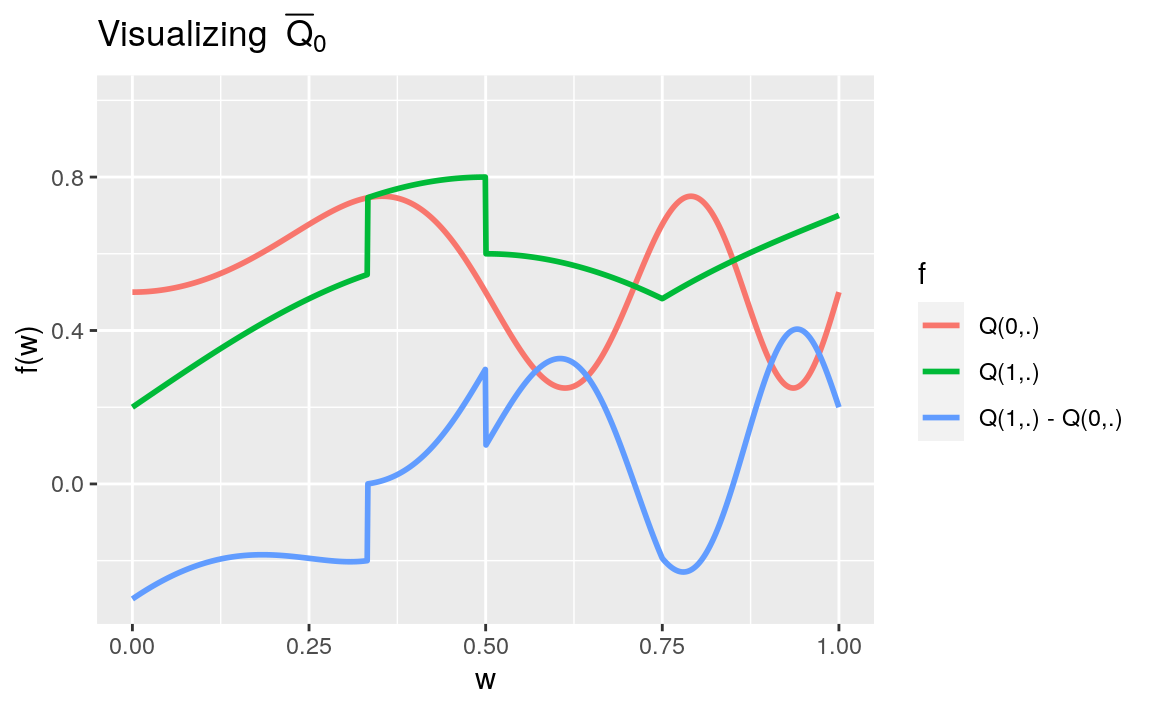
\includegraphics[width=0.7\linewidth]{img/exercise:visualize-1} \end{center}

\begin{enumerate}
\def\labelenumi{\arabic{enumi}.}
\setcounter{enumi}{1}
\tightlist
\item
  Adapt the above chunk of code to visualize the marginal density \(Q_{0,W}\)
  and conditional probability \(\Gbar_{0}\).
\end{enumerate}

\hypertarget{exo-make-own-experiment}{%
\section{\texorpdfstring{⚙ \gear Make your own experiment}{⚙ Make your own experiment}}\label{exo-make-own-experiment}}

You can easily make your own experiment.

\begin{enumerate}
\def\labelenumi{\arabic{enumi}.}
\item
  Check out the man page of method \texttt{alter} by running \texttt{?alter}.
\item
  Run the following chunk of code:
\end{enumerate}

\begin{Shaded}
\begin{Highlighting}[]
\NormalTok{my\_experiment }\OtherTok{\textless{}{-}} \FunctionTok{LAW}\NormalTok{() }\DocumentationTok{\#\# creates an object of class \textquotesingle{}LAW\textquotesingle{}}
\FunctionTok{alter}\NormalTok{(my\_experiment,   }\DocumentationTok{\#\# characterize its relevant features}
      \AttributeTok{QW =} \FunctionTok{tribble}\NormalTok{(}
        \SpecialCharTok{\textasciitilde{}}\NormalTok{value, }\SpecialCharTok{\textasciitilde{}}\NormalTok{weight,}
        \DecValTok{0}\NormalTok{, }\DecValTok{1}\SpecialCharTok{/}\DecValTok{4}\NormalTok{, }\DocumentationTok{\#\# the probabilities must...}
        \DecValTok{1}\NormalTok{, }\DecValTok{3}\SpecialCharTok{/}\DecValTok{4}  \DocumentationTok{\#\# ... sum up to 1}
\NormalTok{      ),}
      \AttributeTok{Gbar =} \ControlFlowTok{function}\NormalTok{(W) \{}
\NormalTok{        out }\OtherTok{\textless{}{-}} \FunctionTok{rep\_len}\NormalTok{(}\DecValTok{0}\NormalTok{, }\FunctionTok{length}\NormalTok{(W))}
\NormalTok{        out[W }\SpecialCharTok{==} \DecValTok{0}\NormalTok{] }\OtherTok{\textless{}{-}} \DecValTok{1}\SpecialCharTok{/}\DecValTok{3}
\NormalTok{        out[W }\SpecialCharTok{==} \DecValTok{1}\NormalTok{] }\OtherTok{\textless{}{-}} \DecValTok{3}\SpecialCharTok{/}\DecValTok{5}
        \FunctionTok{return}\NormalTok{(out)}
\NormalTok{      \},}
      \AttributeTok{Qbar =} \ControlFlowTok{function}\NormalTok{(AW) \{}
\NormalTok{        probs }\OtherTok{\textless{}{-}} \FunctionTok{matrix}\NormalTok{(}\FunctionTok{c}\NormalTok{(}\DecValTok{1}\SpecialCharTok{/}\DecValTok{2}\NormalTok{, }\DecValTok{2}\SpecialCharTok{/}\DecValTok{3}\NormalTok{, }\DecValTok{7}\SpecialCharTok{/}\DecValTok{8}\NormalTok{, }\DecValTok{4}\SpecialCharTok{/}\DecValTok{5}\NormalTok{), }\AttributeTok{ncol =} \DecValTok{2}\NormalTok{,}
                        \AttributeTok{dimnames =} \FunctionTok{list}\NormalTok{(}\FunctionTok{c}\NormalTok{(}\StringTok{"A=0"}\NormalTok{, }\StringTok{"A=1"}\NormalTok{),}
                                        \FunctionTok{c}\NormalTok{(}\StringTok{"W=0"}\NormalTok{, }\StringTok{"W=1"}\NormalTok{)))}
\NormalTok{        probs[}\FunctionTok{cbind}\NormalTok{(AW[, }\StringTok{"A"}\NormalTok{] }\SpecialCharTok{+} \DecValTok{1}\NormalTok{, AW[, }\StringTok{"W"}\NormalTok{] }\SpecialCharTok{+} \DecValTok{1}\NormalTok{)]}
\NormalTok{      \},}
      \AttributeTok{qY =} \ControlFlowTok{function}\NormalTok{(obs) \{}
\NormalTok{        probs }\OtherTok{\textless{}{-}} \FunctionTok{matrix}\NormalTok{(}\FunctionTok{c}\NormalTok{(}\DecValTok{1}\SpecialCharTok{/}\DecValTok{2}\NormalTok{, }\DecValTok{2}\SpecialCharTok{/}\DecValTok{3}\NormalTok{, }\DecValTok{7}\SpecialCharTok{/}\DecValTok{8}\NormalTok{, }\DecValTok{4}\SpecialCharTok{/}\DecValTok{5}\NormalTok{), }\AttributeTok{ncol =} \DecValTok{2}\NormalTok{,}
                        \AttributeTok{dimnames =} \FunctionTok{list}\NormalTok{(}\FunctionTok{c}\NormalTok{(}\StringTok{"A=0"}\NormalTok{, }\StringTok{"A=1"}\NormalTok{),}
                                        \FunctionTok{c}\NormalTok{(}\StringTok{"W=0"}\NormalTok{, }\StringTok{"W=1"}\NormalTok{)))}
\NormalTok{        probs }\OtherTok{\textless{}{-}}\NormalTok{ probs[}\FunctionTok{cbind}\NormalTok{(obs[, }\StringTok{"A"}\NormalTok{] }\SpecialCharTok{+} \DecValTok{1}\NormalTok{, obs[, }\StringTok{"W"}\NormalTok{] }\SpecialCharTok{+} \DecValTok{1}\NormalTok{)]}
\NormalTok{        obs[, }\StringTok{"Y"}\NormalTok{] }\SpecialCharTok{*}\NormalTok{ probs }\SpecialCharTok{+}\NormalTok{ (}\DecValTok{1} \SpecialCharTok{{-}}\NormalTok{ obs[, }\StringTok{"Y"}\NormalTok{]) }\SpecialCharTok{*}\NormalTok{ (}\DecValTok{1} \SpecialCharTok{{-}}\NormalTok{ probs)}
\NormalTok{      \},}
      \AttributeTok{sample\_from =} \ControlFlowTok{function}\NormalTok{(n) \{}
        \DocumentationTok{\#\# preliminary}
\NormalTok{        n }\OtherTok{\textless{}{-}}\NormalTok{ R.utils}\SpecialCharTok{::}\NormalTok{Arguments}\SpecialCharTok{$}\FunctionTok{getInteger}\NormalTok{(n, }\FunctionTok{c}\NormalTok{(}\DecValTok{1}\NormalTok{, }\ConstantTok{Inf}\NormalTok{))}
        \DocumentationTok{\#\# \textquotesingle{}QW\textquotesingle{}, \textquotesingle{}Gbar\textquotesingle{} and \textquotesingle{}Qbar\textquotesingle{} features}
\NormalTok{        QW }\OtherTok{\textless{}{-}}\NormalTok{ my\_experiment}\SpecialCharTok{$}\NormalTok{.QW}
\NormalTok{        Gbar }\OtherTok{\textless{}{-}}\NormalTok{ my\_experiment}\SpecialCharTok{$}\NormalTok{.Gbar}
\NormalTok{        Qbar }\OtherTok{\textless{}{-}}\NormalTok{ my\_experiment}\SpecialCharTok{$}\NormalTok{.Qbar}
        \DocumentationTok{\#\# sampling}
\NormalTok{        W }\OtherTok{\textless{}{-}} \FunctionTok{rbinom}\NormalTok{(n, }\AttributeTok{size =} \DecValTok{1}\NormalTok{, }\AttributeTok{prob =}\NormalTok{ QW}\SpecialCharTok{$}\NormalTok{weight[QW}\SpecialCharTok{$}\NormalTok{value }\SpecialCharTok{==} \DecValTok{1}\NormalTok{])}
\NormalTok{        A }\OtherTok{\textless{}{-}} \FunctionTok{rbinom}\NormalTok{(n, }\AttributeTok{size =} \DecValTok{1}\NormalTok{, }\AttributeTok{prob =} \FunctionTok{Gbar}\NormalTok{(W))}
\NormalTok{        AW }\OtherTok{\textless{}{-}} \FunctionTok{cbind}\NormalTok{(}\AttributeTok{W =}\NormalTok{ W, }\AttributeTok{A =}\NormalTok{ A)}
\NormalTok{        Y }\OtherTok{\textless{}{-}} \FunctionTok{rbinom}\NormalTok{(n, }\AttributeTok{size =} \DecValTok{1}\NormalTok{, }\FunctionTok{Qbar}\NormalTok{(AW))}
        \FunctionTok{return}\NormalTok{(}\FunctionTok{cbind}\NormalTok{(AW, }\AttributeTok{Y =}\NormalTok{ Y))}
\NormalTok{      \})}
\end{Highlighting}
\end{Shaded}

Note that the \texttt{QW} feature of \texttt{my\_experiment} is a \texttt{tibble}, contrary to the
\texttt{QW} feature of \texttt{experiment} which is a \texttt{function}. The former describes a
discrete law and the latter is a density. Those are the two configurations
handled by the package.

\begin{enumerate}
\def\labelenumi{\arabic{enumi}.}
\setcounter{enumi}{2}
\tightlist
\item
  What does the next chunk do?
\end{enumerate}

\begin{Shaded}
\begin{Highlighting}[]
\NormalTok{(}\FunctionTok{sample\_from}\NormalTok{(my\_experiment, }\DecValTok{3}\NormalTok{))}
\CommentTok{\#\textgreater{}      W A Y}
\CommentTok{\#\textgreater{} [1,] 0 1 1}
\CommentTok{\#\textgreater{} [2,] 1 0 1}
\CommentTok{\#\textgreater{} [3,] 1 0 1}
\end{Highlighting}
\end{Shaded}

\begin{enumerate}
\def\labelenumi{\arabic{enumi}.}
\setcounter{enumi}{3}
\tightlist
\item
  Characterize entirely the law of \texttt{my\_experiment}. Hint:
\end{enumerate}

\begin{Shaded}
\begin{Highlighting}[]
\NormalTok{obs }\OtherTok{\textless{}{-}} \FunctionTok{sample\_from}\NormalTok{(my\_experiment, }\FloatTok{1e4}\NormalTok{)}
\NormalTok{obs }\SpecialCharTok{\%\textgreater{}\%}\NormalTok{ as\_tibble }\SpecialCharTok{\%\textgreater{}\%} \FunctionTok{group\_by}\NormalTok{(W, A, Y) }\SpecialCharTok{\%\textgreater{}\%}
  \FunctionTok{summarize}\NormalTok{(}\AttributeTok{how\_many =} \FunctionTok{n}\NormalTok{(), }\AttributeTok{.groups =} \StringTok{"drop"}\NormalTok{)}
\CommentTok{\#\textgreater{} \# A tibble: 8 x 4}
\CommentTok{\#\textgreater{}       W     A     Y how\_many}
\CommentTok{\#\textgreater{}   \textless{}int\textgreater{} \textless{}int\textgreater{} \textless{}int\textgreater{}    \textless{}int\textgreater{}}
\CommentTok{\#\textgreater{} 1     0     0     0      841}
\CommentTok{\#\textgreater{} 2     0     0     1      876}
\CommentTok{\#\textgreater{} 3     0     1     0      264}
\CommentTok{\#\textgreater{} 4     0     1     1      497}
\CommentTok{\#\textgreater{} 5     1     0     0      370}
\CommentTok{\#\textgreater{} 6     1     0     1     2668}
\CommentTok{\#\textgreater{} \# ... with 2 more rows}
\NormalTok{obs }\SpecialCharTok{\%\textgreater{}\%}\NormalTok{ as\_tibble }\SpecialCharTok{\%\textgreater{}\%} 
  \FunctionTok{summarize}\NormalTok{(}\StringTok{"P(W=1)"} \OtherTok{=} \FunctionTok{mean}\NormalTok{(W))}
\CommentTok{\#\textgreater{} \# A tibble: 1 x 1}
\CommentTok{\#\textgreater{}   \textasciigrave{}P(W=1)\textasciigrave{}}
\CommentTok{\#\textgreater{}      \textless{}dbl\textgreater{}}
\CommentTok{\#\textgreater{} 1    0.752}
\NormalTok{obs }\SpecialCharTok{\%\textgreater{}\%}\NormalTok{ as\_tibble }\SpecialCharTok{\%\textgreater{}\%} \FunctionTok{group\_by}\NormalTok{(W) }\SpecialCharTok{\%\textgreater{}\%}
  \FunctionTok{summarize}\NormalTok{(}\StringTok{"P(A=1|W)"} \OtherTok{=} \FunctionTok{mean}\NormalTok{(A))}
\CommentTok{\#\textgreater{} \# A tibble: 2 x 2}
\CommentTok{\#\textgreater{}       W \textasciigrave{}P(A=1|W)\textasciigrave{}}
\CommentTok{\#\textgreater{}   \textless{}int\textgreater{}      \textless{}dbl\textgreater{}}
\CommentTok{\#\textgreater{} 1     0      0.307}
\CommentTok{\#\textgreater{} 2     1      0.596}
\NormalTok{obs }\SpecialCharTok{\%\textgreater{}\%}\NormalTok{ as\_tibble }\SpecialCharTok{\%\textgreater{}\%} \FunctionTok{group\_by}\NormalTok{(W, A) }\SpecialCharTok{\%\textgreater{}\%}
  \FunctionTok{summarize}\NormalTok{(}\StringTok{"P(Y=1|A,W)"} \OtherTok{=} \FunctionTok{mean}\NormalTok{(Y), }\AttributeTok{.groups =} \StringTok{"drop"}\NormalTok{)}
\CommentTok{\#\textgreater{} \# A tibble: 4 x 3}
\CommentTok{\#\textgreater{}       W     A \textasciigrave{}P(Y=1|A,W)\textasciigrave{}}
\CommentTok{\#\textgreater{}   \textless{}int\textgreater{} \textless{}int\textgreater{}        \textless{}dbl\textgreater{}}
\CommentTok{\#\textgreater{} 1     0     0        0.510}
\CommentTok{\#\textgreater{} 2     0     1        0.653}
\CommentTok{\#\textgreater{} 3     1     0        0.878}
\CommentTok{\#\textgreater{} 4     1     1        0.806}
\end{Highlighting}
\end{Shaded}

\begin{enumerate}
\def\labelenumi{\arabic{enumi}.}
\setcounter{enumi}{4}
\tightlist
\item
  Now, make your own experiment.
\end{enumerate}

\hypertarget{parameter}{%
\chapter{The parameter of interest}\label{parameter}}

\hypertarget{parameter-first-pass}{%
\section{The parameter of interest}\label{parameter-first-pass}}

\hypertarget{definition}{%
\subsection{Definition}\label{definition}}

It happens that we especially care for a finite-dimensional feature of \(P_{0}\)
that we denote by \(\psi_{0}\). Its definition involves two of the
aforementioned infinite-dimensional features, the marginal law \(Q_{0,W}\) of
\(W\) and the conditional mean \(\Qbar_{0}\) of \(Y\) given \(A\) and \(W\):
\begin{align}  \psi_{0}  &\defq  \int \left(\Qbar_{0}(1,  w)  -  \Qbar_{0}(0,
w)\right)    dQ_{0,W}(w)    \label{eq:psi-zero}\\     \notag    &=    \Exp_{P_{0}}
\left(\Exp_{P_0}(Y \mid  A =  1, W)  - \Exp_{P_0}(Y  \mid A  = 0,  W) \right).
\end{align}

Acting as oracles, we can compute explicitly the numerical value of
\(\psi_{0}\). The \texttt{evaluate\_psi} method makes it very easy (simply run
\texttt{?estimate\_psi} to see the man page of the method):

\begin{Shaded}
\begin{Highlighting}[]
\NormalTok{(psi\_zero }\OtherTok{\textless{}{-}} \FunctionTok{evaluate\_psi}\NormalTok{(experiment))}
\CommentTok{\#\textgreater{} [1] 0.0832}
\end{Highlighting}
\end{Shaded}

\hypertarget{causal-interpretation}{%
\subsection{A causal interpretation}\label{causal-interpretation}}

Our interest in \(\psi_{0}\) is of causal nature. Taking a closer look at the
\texttt{sample\_from} feature of \texttt{experiment} reveals indeed that the random making of
an observation \(O\) drawn from \(P_{0}\) can be summarized by the following
directed acyclic graph:



\begin{Shaded}
\begin{Highlighting}[]
\FunctionTok{dagify}\NormalTok{(}
\NormalTok{  Y }\SpecialCharTok{\textasciitilde{}}\NormalTok{ A }\SpecialCharTok{+}\NormalTok{ Y1 }\SpecialCharTok{+}\NormalTok{ Y0, A }\SpecialCharTok{\textasciitilde{}}\NormalTok{ W, Y1 }\SpecialCharTok{\textasciitilde{}}\NormalTok{ W, Y0 }\SpecialCharTok{\textasciitilde{}}\NormalTok{ W,}
  \AttributeTok{labels =} \FunctionTok{c}\NormalTok{(}\AttributeTok{Y =} \StringTok{"Actual reward"}\NormalTok{,}
             \AttributeTok{A =} \StringTok{"Action"}\NormalTok{,}
             \AttributeTok{Y1 =} \StringTok{"Counterfactual reward}\SpecialCharTok{\textbackslash{}n}\StringTok{ of action 1"}\NormalTok{,}
             \AttributeTok{Y0 =} \StringTok{"Counterfactual reward}\SpecialCharTok{\textbackslash{}n}\StringTok{ of action 0"}\NormalTok{,}
             \AttributeTok{W =} \StringTok{"Context of action"}\NormalTok{),}
  \AttributeTok{coords =} \FunctionTok{list}\NormalTok{(}
    \AttributeTok{x =} \FunctionTok{c}\NormalTok{(}\AttributeTok{W =} \DecValTok{0}\NormalTok{, }\AttributeTok{A =} \SpecialCharTok{{-}}\DecValTok{1}\NormalTok{, }\AttributeTok{Y1 =} \FloatTok{1.5}\NormalTok{, }\AttributeTok{Y0 =} \FloatTok{0.25}\NormalTok{, }\AttributeTok{Y =} \DecValTok{1}\NormalTok{),}
    \AttributeTok{y =} \FunctionTok{c}\NormalTok{(}\AttributeTok{W =} \DecValTok{0}\NormalTok{, }\AttributeTok{A =} \SpecialCharTok{{-}}\DecValTok{1}\NormalTok{, }\AttributeTok{Y1 =} \SpecialCharTok{{-}}\FloatTok{0.5}\NormalTok{, }\AttributeTok{Y0 =} \SpecialCharTok{{-}}\FloatTok{0.5}\NormalTok{, }\AttributeTok{Y =} \SpecialCharTok{{-}}\DecValTok{1}\NormalTok{)),}
  \AttributeTok{outcome =} \StringTok{"Y"}\NormalTok{,}
  \AttributeTok{exposure =} \StringTok{"A"}\NormalTok{,}
  \AttributeTok{latent =} \FunctionTok{c}\NormalTok{(}\StringTok{"Y0"}\NormalTok{, }\StringTok{"Y1"}\NormalTok{)) }\SpecialCharTok{\%\textgreater{}\%}\NormalTok{ tidy\_dagitty }\SpecialCharTok{\%\textgreater{}\%}
  \FunctionTok{ggdag}\NormalTok{(}\AttributeTok{text =} \ConstantTok{TRUE}\NormalTok{, }\AttributeTok{use\_labels =} \StringTok{"label"}\NormalTok{) }\SpecialCharTok{+} \FunctionTok{theme\_dag\_grey}\NormalTok{()}
\end{Highlighting}
\end{Shaded}

\begin{figure}

{\centering 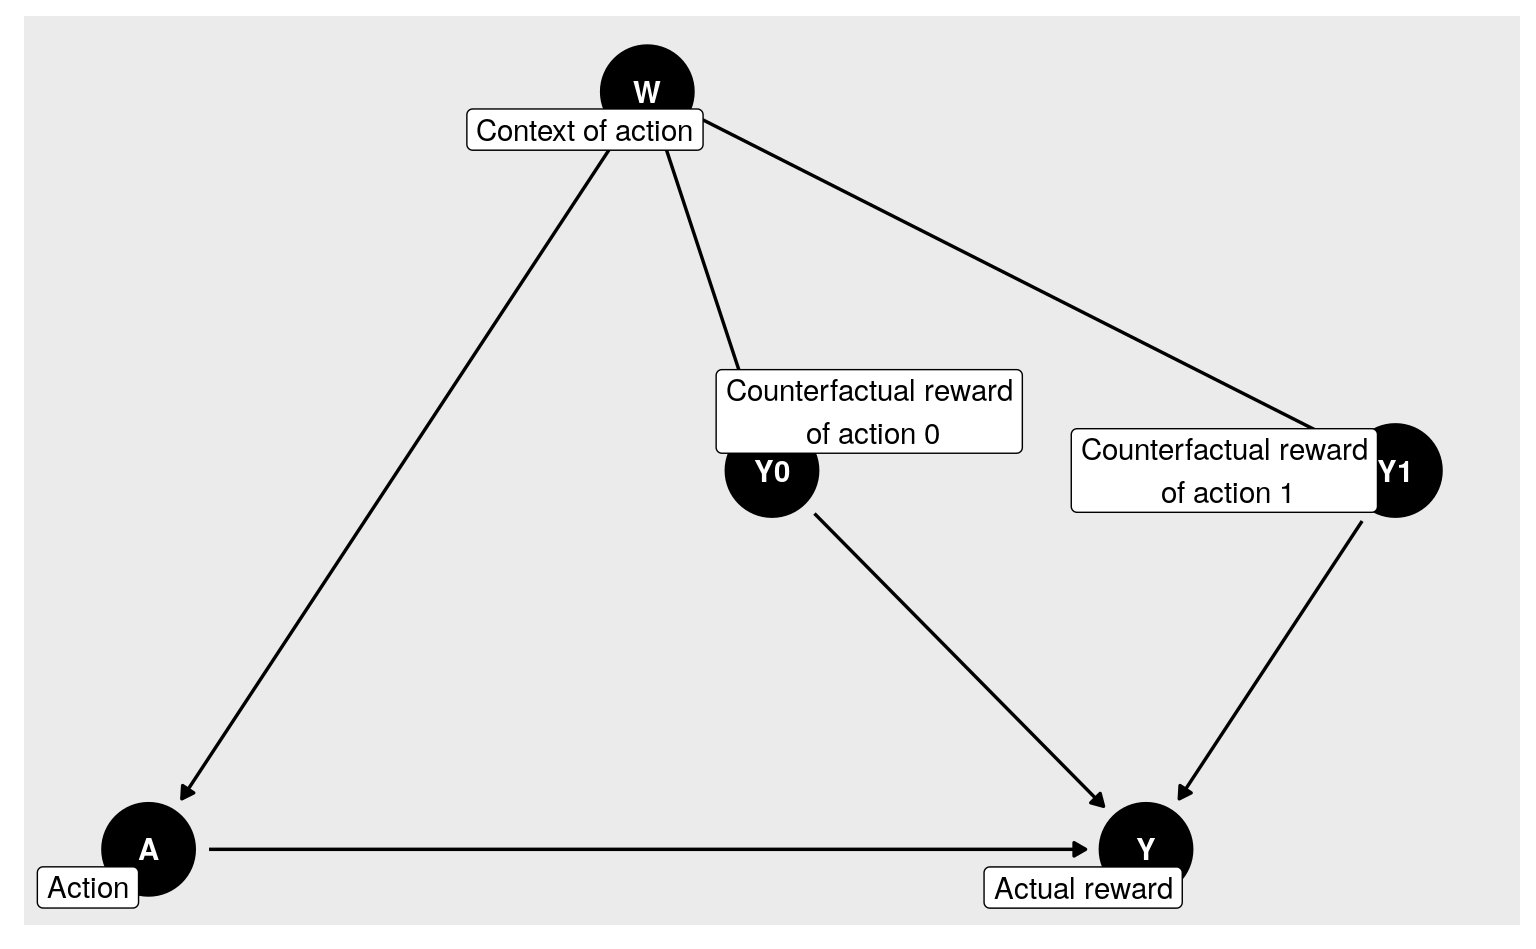
\includegraphics[width=0.7\linewidth]{img/DAG-1} 

}

\caption{Directed acyclic graph summarizing the inner causal mechanism at play in \texttt{experiment}.}\label{fig:DAG}
\end{figure}

In words, the experiment unfolds like this (see also Section \ref{npsem}):

\begin{enumerate}
\def\labelenumi{\arabic{enumi}.}
\item
  a context of action \(W \in [0,1]\) is randomly generated;
\item
  two counterfactual rewards \(Y_{0}\in [0,1]\) and \(Y_{1}\in [0,1]\) are
  generated conditionally on \(W\);
\item
  an action \(A \in \{0,1\}\) (among two possible actions called \(a=0\) and
  \(a=1\)) is undertaken, \emph{(i)} knowing the context but \emph{not} the
  counterfactual rewards, and \emph{(ii)} in such a way that both actions can
  always be considered;
\item
  the action yields a reward \(Y\), which equals either \(Y_{0}\) or \(Y_{1}\)
  depending on whether action \(a=0\) or \(a=1\) has been undertaken;
\item
  summarize the course of the experiment with \(O \defq (W, A, Y)\), thus
  concealing \(Y_{0}\) and \(Y_{1}\).
\end{enumerate}

The above description of the experiment is useful to reinforce what it means
to run the ``ideal'' experiment by setting argument \texttt{ideal} to \texttt{TRUE} in a call
to \texttt{sample\_from} for \texttt{experiment} (see Section \ref{causal-computation}).
Doing so triggers a modification of the nature of the experiment, enforcing
that the counterfactual rewards \(Y_{0}\) and \(Y_{1}\) be part of the summary of
the experiment eventually. In light of the above enumeration,
\begin{equation*}  \bbO \defq  (W,  Y_{0}, Y_{1},  A,  Y) \end{equation*} is
output, as opposed to its summary measure \(O\). This defines another
experiment and its law, that we denote \(\bbP_{0}\).

It is straightforward to \protect\hyperlink{identification}{show that}

\begin{align}
\psi_{0} &= \Exp_{\bbP_{0}} \left(Y_{1} - Y_{0}\right) \label{eq:psi-zero-bis} \\
&= \Exp_{\bbP_{0}}(Y_1) - \Exp_{\bbP_{0}}(Y_0).  \notag 
\end{align}

Thus, \(\psi_{0}\) describes the average difference of the two counterfactual
rewards. In other words, \(\psi_{0}\) quantifies the difference in average of
the reward one would get in a world where one would always enforce action
\(a=1\) with the reward one would get in a world where one would always enforce
action \(a=0\). This said, it is worth emphasizing that \(\psi_{0}\) is a
well-defined parameter beyond its causal interpretation, and that it describes
a standardized association between the action \(A\) and reward \(Y\).

\hypertarget{causal-computation}{%
\subsection{A causal computation}\label{causal-computation}}

We can use our position as oracles to sample observations from the ideal
experiment. We call \texttt{sample\_from} for \texttt{experiment} with its argument \texttt{ideal}
set to \texttt{TRUE} in order to numerically approximate \(\psi_{0}\). By the law of
large numbers, the following code approximates \(\psi_{0}\) and shows it
approximate value.

\begin{Shaded}
\begin{Highlighting}[]
\NormalTok{B }\OtherTok{\textless{}{-}} \FloatTok{1e6}
\NormalTok{ideal\_obs }\OtherTok{\textless{}{-}} \FunctionTok{sample\_from}\NormalTok{(experiment, B, }\AttributeTok{ideal =} \ConstantTok{TRUE}\NormalTok{)}
\NormalTok{(psi\_approx }\OtherTok{\textless{}{-}} \FunctionTok{mean}\NormalTok{(ideal\_obs[, }\StringTok{"Yone"}\NormalTok{] }\SpecialCharTok{{-}}\NormalTok{ ideal\_obs[, }\StringTok{"Yzero"}\NormalTok{]))}
\CommentTok{\#\textgreater{} [1] 0.0829}
\end{Highlighting}
\end{Shaded}

The object \texttt{psi\_approx} contains an approximation to \(\psi_0\) based on \texttt{B}
observations from the ideal experiment. The random sampling of observations
results in uncertainty in the numerical approximation of \(\psi_0\). This
uncertainty can be quantified by constructing a 95\% confidence interval for
\(\psi_0\). The central limit theorem and Slutsky's lemma \protect\hyperlink{clt}{allow us} to
build such an interval as follows.

\begin{Shaded}
\begin{Highlighting}[]
\NormalTok{sd\_approx }\OtherTok{\textless{}{-}} \FunctionTok{sd}\NormalTok{(ideal\_obs[, }\StringTok{"Yone"}\NormalTok{] }\SpecialCharTok{{-}}\NormalTok{ ideal\_obs[, }\StringTok{"Yzero"}\NormalTok{])}
\NormalTok{alpha }\OtherTok{\textless{}{-}} \FloatTok{0.05}
\NormalTok{(psi\_approx\_CI }\OtherTok{\textless{}{-}}\NormalTok{ psi\_approx }\SpecialCharTok{+} \FunctionTok{c}\NormalTok{(}\SpecialCharTok{{-}}\DecValTok{1}\NormalTok{, }\DecValTok{1}\NormalTok{) }\SpecialCharTok{*}
   \FunctionTok{qnorm}\NormalTok{(}\DecValTok{1} \SpecialCharTok{{-}}\NormalTok{ alpha }\SpecialCharTok{/} \DecValTok{2}\NormalTok{) }\SpecialCharTok{*}\NormalTok{ sd\_approx }\SpecialCharTok{/} \FunctionTok{sqrt}\NormalTok{(B))}
\CommentTok{\#\textgreater{} [1] 0.0823 0.0835}
\end{Highlighting}
\end{Shaded}

We note that the interpretation of this confidence interval is that in 95\% of
draws of size \texttt{B} from the ideal data generating experiment, the true value of
\(\psi_0\) will be contained in the generated confidence interval.

\hypertarget{exo-alternative-parameter-first-pass}{%
\section{\texorpdfstring{⚙ \gear An alternative parameter of interest}{⚙ An alternative parameter of interest}}\label{exo-alternative-parameter-first-pass}}

Equality \eqref{eq:psi-zero-bis} shows that parameter \(\psi_0\)
\eqref{eq:psi-zero} is the difference in average rewards if we enforce action
\(a = 1\) rather than \(a = 0\). An alternative way to describe the rewards under
different actions involves \emph{quantiles} as opposed to \emph{averages}.

Let \begin{equation*} Q_{0,Y}(y,  A, W) \defq \int_{0}^y q_{0,Y}(u,  A, W) du
\end{equation*} be the conditional cumulative distribution of reward \(Y\) given
\(A\) and \(W\), evaluated at \(y \in ]0,1[\), that is implied by \(P_0\). For each
action \(a \in \{0,1\}\) and \(c \in ]0,1[\), introduce

\begin{equation}
\gamma_{0,a,c}  \defq  \inf  \left\{y  \in  ]0,1[ :  \int  Q_{0,Y}(y,  a,  w)
dQ_{0,W}(w) \ge c \right\}. \label{eq:def-quantile}
\end{equation}
(Note: \(\inf\) merely generalizes \(\min\), accounting for the fact that the
minimum may fail to be achieved.)

It is not very difficult to check (see Problem 1 below) that
\begin{equation}\gamma_{0,a,c} =  \inf\left\{y \in ]0,1[  : \Pr_{\bbP_{0}}(Y_a
\leq   y)   \geq   c\right\}.    \label{eq:alter-gamma-zero}\end{equation} Thus,
\(\gamma_{0,a,c}\) can be interpreted as the \(c\)-th quantile
reward when action \(a\) is enforced. The difference
\begin{equation}\delta_{0,c}    \defq    \gamma_{0,1,c}   -    \gamma_{0,0,c}
\label{eq:def-delta}\end{equation} is the \(c\)-th quantile counterpart to parameter
\(\psi_{0}\) \eqref{eq:psi-zero}.

\begin{enumerate}
\def\labelenumi{\arabic{enumi}.}
\item
  ☡ \stixdanger{} Prove \eqref{eq:alter-gamma-zero}.
\item
  ☡ \stixdanger{} Compute the numerical value of \(\gamma_{0,a,c}\) for each \((a,c) \in \{0,1\} \times \{1/4, 1/2, 3/4\}\) using the appropriate features of
  \texttt{experiment} (see \texttt{relevant\_features}). Based on these results, report the
  numerical value of \(\delta_{0,c}\) for each \(c \in \{1/4, 1/2, 3/4\}\).
\item
  Approximate the numerical values of \(\gamma_{0,a,c}\) for each \((a,c) \in \{0,1\} \times \{1/4, 1/2, 3/4\}\) by drawing a large sample from the
  ``ideal'' data experiment and using empirical quantile estimates. Deduce
  from these results a numerical approximation to \(\delta_{0,c}\) for \(c \in \{1/4, 1/2, 3/4\}\). Confirm that your results closely match those obtained
  in the previous problem.
\end{enumerate}

\hypertarget{parameter-second-pass}{%
\section{The statistical mapping of interest}\label{parameter-second-pass}}

The noble way to define a statistical parameter is to view it as the value of
a statistical mapping at the law of the experiment of interest. Beyond the
elegance, this has paramount statistical implications.

\hypertarget{opening}{%
\subsection{Opening discussion}\label{opening}}

Oftentimes, the premise of a statistical analysis is presented like this. One
assumes that the law \(P_{0}\) of the experiment of interest belongs to a
statistical model \begin{equation*}\{P_{\theta}     :    \theta     \in
T\}\end{equation*} (where \(T\) is some index set). The statistical model is identifiable, meaning that if two
elements \(P_{\theta}\) and \(P_{\theta'}\) coincide, then necessarily \(\theta = \theta'\). Therefore, there exists a unique \(\theta_{0} \in T\) such that
\(P_{0} = P_{\theta_{0}}\), and one wishes to estimate
\(\theta_{0}\).\index{identifiability}

For instance, each \(P_{\theta}\) could be the Gaussian law with mean \(\theta \in T \defq \bbR\) and variance 1, and one could wish to estimate the mean
\(\theta_{0}\) of \(P_{0}\). To do so, one could rely on \(n\) observations \(X_{1}\),
\ldots, \(X_{n}\) drawn independently from \(P_{0}\). The empirical mean
\begin{equation*}\theta_{n}       \defq      \frac{1}{n}       \sum_{i=1}^{n}
X_{i}\end{equation*} estimates \(\theta_{0}\). More generally, if we assume that \(\Var_{P_{0}} (X_{1})\) is finite, then \(\theta_{n}\) satisfies many useful properties. In
particular, it can be used \protect\hyperlink{clt}{to construct confidence intervals}.

Of course, the mean of a law is defined beyond the small model \(\{P_{\theta} : \theta \in \bbR\}\). Let \(\calM\) be the set of laws \(P\) on \(\bbR\) such that
\(\Var_{P}(X)\) is finite. In particular, \(P_{0} \in \calM\). For every \(P \in \calM\), the mean \(\Exp_{P}(X)\) is well defined. Thus, we can introduce the
\emph{statistical mapping} \(\Theta : \calM \to \bbR\) given by
\begin{equation*}\Theta(P) \defq \Exp_{P}(X).\end{equation*}

Interestingly, the empirical measure \(P_{n}\)\footnote{The empirical measure \(P_{n}\) is
  the law such that \emph{(i)} \(X\) drawn from \(P_{n}\) takes its values in \(\{X_{1}, \ldots, X_{n}\}\), and \emph{(ii)} \(X=X_{i}\) with probability \(n^{-1}\)} is an
element of \(\calM\). Therefore, the statistical mapping \(\Theta\) can be
evaluated at \(P_{n}\): \begin{equation*}\Theta(P_{n})    =   \frac{1}{n}
\sum_{i=1}^{n} X_{i}  = \theta_{n}.\end{equation*} We \emph{recover} the empirical
mean, and understand that it is a \emph{substitution} estimator of the mean: in
order to estimate \(\Theta(P_{0})\), we \emph{substitute} \(P_{n}\) for \(P_{0}\) within
\(\Theta\).\footnote{There are many interesting parameters \(\Theta\) for which
  \(\Theta(P_n)\) is not defined, see for instance \eqref{eq:psimap}, our parameter
  of main interest.}

Substitution-based estimators are particularly valuable notably because they,
by construction, satisfy all the constraints to which the targeted parameter
is subjected. For example, if \(X\) is a binary random variable and the support
of all distributions in our model is \(\{0,1\}\), then \(\Theta\) can be
interpreted as the probability that \(X = 1\), a quantity known to live in the
interval \([0,1]\). A substitution estimator will also be guaranteed to fall
into this interval. Some of the estimators that we will build together are
substitution-based, some are not.

\hypertarget{parameter-mapping}{%
\subsection{The parameter as the value of a statistical mapping at the experiment}\label{parameter-mapping}}

We now go back to our main topic of interest. Suppose we know beforehand that
\(O\) drawn from \(P_{0}\) takes its values in \(\calO \defq [0,1] \times \{0,1\} \times [0,1]\) and that \(\Gbar_{0}(W) \defq \Pr_{P_{0}}(A=1|W)\) is bounded away from
zero and one \(Q_{0,W}\)-almost surely (this is the case indeed). Then we can
define model \(\calM\) as the set of all laws \(P\) on \(\calO\) such that
\begin{equation*}\Gbar(W)  \defq \Pr_{P}(A=1|W)\end{equation*} is bounded away
from zero and one \(Q_{W}\)-almost surely, where \(Q_{W}\) is the marginal law of
\(W\) under \(P\).

Let us also define generically \(\Qbar\) as \begin{equation*}\Qbar (A,W) \defq
\Exp_{P} (Y|A, W).\end{equation*} Note how we have suppressed the dependence
of \(\Gbar\) and \(\Qbar\) on \(P\) for notational simplicity.

Central to our approach is viewing \(\psi_{0}\) as the value at \(P_{0}\) of the
statistical mapping \(\Psi\) from \(\calM\) to \([0,1]\) characterized by
\begin{align}  \Psi(P)  &\defq  \int  \left(\Qbar_P(1,  w)  -  \Qbar_P(0,
w)\right)  dQ_{W}(w)   \label{eq:psimap}\\  &=  \Exp_{P}  \left(\Qbar_P(1,   W)  -
\Qbar_P(0,   W)\right),    \notag   \end{align} a clear extension of
\eqref{eq:psi-zero} where, for once, we make the dependence of \(\Qbar\) on \(P\)
explicit to emphasize how \(\Psi(P)\) truly depends on \(P\).

\hypertarget{value-another-experiment}{%
\subsection{The value of the statistical mapping at another experiment}\label{value-another-experiment}}

When we ran \texttt{example(tlrider)} earlier, we created an object called
\texttt{another\_experiment}:

\begin{Shaded}
\begin{Highlighting}[]
\NormalTok{another\_experiment}
\CommentTok{\#\textgreater{} A law for (W,A,Y) in [0,1] x \{0,1\} x [0,1].}
\CommentTok{\#\textgreater{} }
\CommentTok{\#\textgreater{} If the law is fully characterized, you can use method}
\CommentTok{\#\textgreater{} \textquotesingle{}sample\_from\textquotesingle{} to sample from it.}
\CommentTok{\#\textgreater{} }
\CommentTok{\#\textgreater{} If you built the law, or if you are an \_oracle\_, you can also}
\CommentTok{\#\textgreater{} use methods \textquotesingle{}reveal\textquotesingle{} to reveal its relevant features (QW, Gbar,}
\CommentTok{\#\textgreater{} Qbar, qY {-}{-} see \textquotesingle{}?reveal\textquotesingle{}), and \textquotesingle{}alter\textquotesingle{} to change some of them.}
\CommentTok{\#\textgreater{} }
\CommentTok{\#\textgreater{} If all its relevant features are characterized, you can use}
\CommentTok{\#\textgreater{} methods \textquotesingle{}evaluate\_psi\textquotesingle{} to obtain the value of \textquotesingle{}Psi\textquotesingle{} at this law}
\CommentTok{\#\textgreater{} (see \textquotesingle{}?evaluate\_psi\textquotesingle{}) and \textquotesingle{}evaluate\_eic\textquotesingle{} to obtain the efficient}
\CommentTok{\#\textgreater{} influence curve of \textquotesingle{}Psi\textquotesingle{} at this law (see \textquotesingle{}?evaluate\_eic\textquotesingle{}).}
\FunctionTok{reveal}\NormalTok{(another\_experiment)}
\CommentTok{\#\textgreater{} $QW}
\CommentTok{\#\textgreater{} function(x, min = 1/10, max = 9/10)\{}
\CommentTok{\#\textgreater{}              stats::dunif(x, min = min, max = max)}
\CommentTok{\#\textgreater{}       \}}
\CommentTok{\#\textgreater{} \textless{}environment: 0x55d8a59c3748\textgreater{}}
\CommentTok{\#\textgreater{} }
\CommentTok{\#\textgreater{} $Gbar}
\CommentTok{\#\textgreater{} function(W) \{}
\CommentTok{\#\textgreater{}         sin((1 + W) * pi / 6)}
\CommentTok{\#\textgreater{}       \}}
\CommentTok{\#\textgreater{} \textless{}environment: 0x55d8a59c3748\textgreater{}}
\CommentTok{\#\textgreater{} }
\CommentTok{\#\textgreater{} $Qbar}
\CommentTok{\#\textgreater{} function(AW, h) \{}
\CommentTok{\#\textgreater{}         A \textless{}{-} AW[, "A"]}
\CommentTok{\#\textgreater{}         W \textless{}{-} AW[, "W"]}
\CommentTok{\#\textgreater{}         expit( logit( A *  W + (1 {-} A) * W\^{}2 ) +}
\CommentTok{\#\textgreater{}                h * 10 * sqrt(W) * A )}
\CommentTok{\#\textgreater{}       \}}
\CommentTok{\#\textgreater{} \textless{}environment: 0x55d8a59c3748\textgreater{}}
\CommentTok{\#\textgreater{} }
\CommentTok{\#\textgreater{} $qY}
\CommentTok{\#\textgreater{} function(obs, Qbar, shape1 = 4)\{}
\CommentTok{\#\textgreater{}         AW \textless{}{-} obs[, c("A", "W")]}
\CommentTok{\#\textgreater{}         QAW \textless{}{-} Qbar(AW)}
\CommentTok{\#\textgreater{}         stats::gdbeta(Y,}
\CommentTok{\#\textgreater{}                       shape1 = shape1,}
\CommentTok{\#\textgreater{}                       shape2 = shape1 * (1 {-} QAW) / QAW)}
\CommentTok{\#\textgreater{}       \}}
\CommentTok{\#\textgreater{} \textless{}environment: 0x55d8a59c3748\textgreater{}}
\CommentTok{\#\textgreater{} }
\CommentTok{\#\textgreater{} $sample\_from}
\CommentTok{\#\textgreater{} function(n, h) \{}
\CommentTok{\#\textgreater{}         \#\# preliminary}
\CommentTok{\#\textgreater{}         n \textless{}{-} R.utils::Arguments$getInteger(n, c(1, Inf))}
\CommentTok{\#\textgreater{}         h \textless{}{-} R.utils::Arguments$getNumeric(h)}
\CommentTok{\#\textgreater{}         \#\# \#\# \textquotesingle{}Gbar\textquotesingle{} and \textquotesingle{}Qbar\textquotesingle{} factors}
\CommentTok{\#\textgreater{}         Gbar \textless{}{-} another\_experiment$.Gbar}
\CommentTok{\#\textgreater{}         Qbar \textless{}{-} another\_experiment$.Qbar}
\CommentTok{\#\textgreater{}         \#\# sampling}
\CommentTok{\#\textgreater{}         \#\# \#\# context}
\CommentTok{\#\textgreater{}         params \textless{}{-} formals(another\_experiment$.QW)}
\CommentTok{\#\textgreater{}         W \textless{}{-} stats::runif(n, min = eval(params$min),}
\CommentTok{\#\textgreater{}                    max = eval(params$max))}
\CommentTok{\#\textgreater{}         \#\# \#\# action undertaken}
\CommentTok{\#\textgreater{}         A \textless{}{-} stats::rbinom(n, size = 1, prob = Gbar(W))}
\CommentTok{\#\textgreater{}         \#\# \#\# reward}
\CommentTok{\#\textgreater{}         params \textless{}{-} formals(another\_experiment$.qY)}
\CommentTok{\#\textgreater{}         shape1 \textless{}{-} eval(params$shape1)}
\CommentTok{\#\textgreater{}         QAW \textless{}{-} Qbar(cbind(A = A, W = W), h = h)}
\CommentTok{\#\textgreater{}         Y \textless{}{-} stats::rbeta(n,}
\CommentTok{\#\textgreater{}                           shape1 = shape1,}
\CommentTok{\#\textgreater{}                           shape2 = shape1 * (1 {-} QAW) / QAW)}
\CommentTok{\#\textgreater{}         \#\# \#\# observation}
\CommentTok{\#\textgreater{}         obs \textless{}{-} cbind(W = W, A = A, Y = Y)}
\CommentTok{\#\textgreater{}         return(obs)}
\CommentTok{\#\textgreater{}       \}}
\CommentTok{\#\textgreater{} \textless{}environment: 0x55d8a59c3748\textgreater{}}
\NormalTok{(two\_obs\_another\_experiment }\OtherTok{\textless{}{-}} \FunctionTok{sample\_from}\NormalTok{(another\_experiment, }\DecValTok{2}\NormalTok{, }\AttributeTok{h =} \DecValTok{0}\NormalTok{))}
\CommentTok{\#\textgreater{}          W A     Y}
\CommentTok{\#\textgreater{} [1,] 0.720 1 0.372}
\CommentTok{\#\textgreater{} [2,] 0.616 1 0.670}
\end{Highlighting}
\end{Shaded}

By taking an oracular look at the output of \texttt{reveal(another\_experiment)}, we
discover that the law \(\Pi_{0} \in \calM\) encoded by default (\emph{i.e.}, with
\texttt{h=0}) in \texttt{another\_experiment} differs starkly from \(P_{0}\).

However, the parameter \(\Psi(\Pi_{0})\) is well defined. Straightforward
algebra shows that \(\Psi(\Pi_{0}) = 59/300\). The numeric computation below
confirms the equality.

\begin{Shaded}
\begin{Highlighting}[]
\NormalTok{(psi\_Pi\_zero }\OtherTok{\textless{}{-}} \FunctionTok{evaluate\_psi}\NormalTok{(another\_experiment, }\AttributeTok{h =} \DecValTok{0}\NormalTok{))}
\CommentTok{\#\textgreater{} [1] 0.197}
\FunctionTok{round}\NormalTok{(}\DecValTok{59}\SpecialCharTok{/}\DecValTok{300}\NormalTok{, }\DecValTok{3}\NormalTok{)}
\CommentTok{\#\textgreater{} [1] 0.197}
\end{Highlighting}
\end{Shaded}

\hypertarget{exo-alternative-parameter-second-pass}{%
\section{\texorpdfstring{⚙ \gear Alternative statistical mapping}{⚙ Alternative statistical mapping}}\label{exo-alternative-parameter-second-pass}}

We now resume the exercise of Section
\ref{exo-alternative-parameter-first-pass}. Like we did in Section
\ref{parameter-second-pass}, we introduce a generic version of the relevant
features \(q_{0,Y}\) and \(Q_{0,Y}\). Specifically, we define \(q_{Y}(y,A,W)\) to
be the conditional density of \(Y\) given \(A\) and \(W\), evaluated at \(y\), that is
implied by a generic \(P \in \calM\). Similarly, we use \(Q_{Y}\) to denote the
corresponding cumulative distribution function.

The covariate-adjusted \(c\)-th quantile reward for action \(a \in \{0,1\}\),
\(\gamma_{0,a,c}\) \eqref{eq:def-quantile}, may be viewed as the value at \(P_{0}\)
of a mapping \(\Gamma_{a,c}\) from \(\calM\) to \([0,1]\) characterized by
\begin{equation*} \Gamma_{a,c}(P) = \inf\left\{y \in ]0,1[ : \int Q_{Y}(y,a,w)
dQ_W(w) \ge  c \right\}.   \end{equation*} The difference in \(c\)-th quantile
rewards, \(\delta_{0,c}\) \eqref{eq:def-delta}, may similarly be viewed as the
value at \(P_{0}\) of a mapping \(\Delta_c\) from \(\calM\) to \([0,1]\),
characterized by \begin{equation*}   \Delta_c(P)  \defq  \Gamma_{1,c}(P)  -
\Gamma_{0,c}(P).  \end{equation*}

\begin{enumerate}
\def\labelenumi{\arabic{enumi}.}
\item
  Compute the numerical value of \(\Gamma_{a,c}(\Pi_0)\) for \((a,c) \in \{0,1\} \times \{1/4, 1/2, 3/4\}\) using the relevant features of
  \texttt{another\_experiment}. Based on these results, report the numerical value
  of \(\Delta_c(\Pi_0)\) for each \(c \in \{1/4, 1/2, 3/4\}\).
\item
  Approximate the value of \(\Gamma_{0,a,c}(\Pi_{0})\) for \((a,c) \in \{0,1\} \times \{1/4, 1/2, 3/4\}\) by drawing a large sample from the ``ideal'' data
  experiment and using empirical quantile estimates. Deduce from these
  results a numerical approximation to \(\Delta_{0,c} (\Pi_{0})\) for each \(c \in \{1/4, 1/2, 3/4\}\). Confirm that your results closely match those
  obtained in the previous problem.
\item
  Building upon the code you wrote to solve the previous problem, \protect\hyperlink{order}{construct
  a confidence interval} with asymptotic level
  \(95\%\) for \(\Delta_{0,c} (\Pi_{0})\), with \(c \in \{1/4, 1/2, 3/4\}\).
\end{enumerate}

\hypertarget{parameter-third-pass}{%
\section{Representations}\label{parameter-third-pass}}

In Section \ref{parameter-second-pass}, we reoriented our view of the target
parameter to be that of a statistical functional of the law of the observed
data. Specifically, we viewed the parameter as a function of specific features
of the observed data law, namely \(Q_{W}\) and \(\Qbar\).

\hypertarget{yet-another}{%
\subsection{Yet another representation}\label{yet-another}}

It is straightforward to \protect\hyperlink{another-rep}{show an equivalent representation} of
the parameter as

\begin{align}  \notag  \psi_{0}  &=  \int \frac{2a  -  1}{\ell\Gbar_0(a,w)}  y
dP_0(w,a,y)   \\   \label{eq:psi-zero-b}   &=   \Exp_{P_0}   \left(   \frac{2A   -
1}{\ell\Gbar_{0}(A,W)} Y \right).  \end{align} Viewing again the parameter as
a statistical mapping from \(\calM\) to \([0,1]\), it also holds that
\begin{align} \notag  \Psi(P) &= \int \frac{2a-1}{\ell\Gbar(a,w)}  y dP(w,a,y)
\\  \label{eq:psi-zero-c}  &=  \Exp_{P}\left(\frac{2A -  1}{\ell\Gbar_{0}(A,W)}  Y
\right).  \end{align}

\hypertarget{rep-to-est}{%
\subsection{From representations to estimation strategies}\label{rep-to-est}}

Our reason for introducing this alternative view of the target parameter will
become clear when we discuss estimation of the target parameter. Specifically,
the representations \eqref{eq:psi-zero} and \eqref{eq:psi-zero-b} naturally
suggest different estimation strategies for \(\psi_0\), as hinted in Section
\ref{opening}. The former suggests building an estimator of \(\psi_0\) using
estimators of \(\Qbar_0\) and of \(Q_{W,0}\). The latter suggests building an
estimator of \(\psi_0\) using estimators of \(\ell\Gbar_0\) and of \(P_0\).

We return to these ideas in later sections.

\hypertarget{exo-alternative-parameter-third-pass}{%
\section{\texorpdfstring{⚙ \gear Alternative representation}{⚙ Alternative representation}}\label{exo-alternative-parameter-third-pass}}

\begin{enumerate}
\def\labelenumi{\arabic{enumi}.}
\tightlist
\item
  ☡ \stixdanger{} Show that for \(a' = 0,1\), \(\gamma_{0,a',c}\) as defined in
  \eqref{eq:def-quantile} can be equivalently expressed as \begin{equation*}\inf
  \left\{z \in ]0,1[  : \int \frac{\one\{a =  a'\}}{\ell\Gbar(a',W)} \one\{y \le
  z\} dP_0(w,a,y) \ge c \right\}.\end{equation*}
\end{enumerate}

\hypertarget{smooth}{%
\chapter{Smoothness}\label{smooth}}

\hypertarget{smooth-first-pass}{%
\section{Fluctuating smoothly}\label{smooth-first-pass}}

Within our view of the target parameter as a statistical mapping evaluated at
the law of the experiment, it is natural to inquire of properties this
functional enjoys. For example, we may be interested in asking how the value
of \(\Psi(P)\) changes as we consider laws that \emph{get nearer to} \(P\) in \(\calM\).
If small deviations from \(P_0\) result in large changes in \(\Psi(P_0)\), then we
might hypothesize that it will be difficult to produce stable estimators of
\(\psi_0\). Fortunately, this turns out not to be the case for the mapping
\(\Psi\), and so we say that \(\Psi\) is a \emph{smooth} statistical mapping.

To discuss how \(\Psi(P)\) changes for distributions that \emph{get nearer} to \(P\) in
the model, we require a more concrete notion of what it means to \emph{get near} to
a distribution in a model. The notion
hinges on fluctuations (or fluctuating models).

\hypertarget{fluctuations}{%
\subsection{\texorpdfstring{The \texttt{another\_experiment} fluctuation}{The another\_experiment fluctuation}}\label{fluctuations}}

In Section \ref{value-another-experiment}, we discussed the nature of the
object called \texttt{another\_experiment} that was created when we ran
\texttt{example(tlrider)}:

\begin{Shaded}
\begin{Highlighting}[]
\NormalTok{another\_experiment}
\CommentTok{\#\textgreater{} A law for (W,A,Y) in [0,1] x \{0,1\} x [0,1].}
\CommentTok{\#\textgreater{} }
\CommentTok{\#\textgreater{} If the law is fully characterized, you can use method}
\CommentTok{\#\textgreater{} \textquotesingle{}sample\_from\textquotesingle{} to sample from it.}
\CommentTok{\#\textgreater{} }
\CommentTok{\#\textgreater{} If you built the law, or if you are an \_oracle\_, you can also}
\CommentTok{\#\textgreater{} use methods \textquotesingle{}reveal\textquotesingle{} to reveal its relevant features (QW, Gbar,}
\CommentTok{\#\textgreater{} Qbar, qY {-}{-} see \textquotesingle{}?reveal\textquotesingle{}), and \textquotesingle{}alter\textquotesingle{} to change some of them.}
\CommentTok{\#\textgreater{} }
\CommentTok{\#\textgreater{} If all its relevant features are characterized, you can use}
\CommentTok{\#\textgreater{} methods \textquotesingle{}evaluate\_psi\textquotesingle{} to obtain the value of \textquotesingle{}Psi\textquotesingle{} at this law}
\CommentTok{\#\textgreater{} (see \textquotesingle{}?evaluate\_psi\textquotesingle{}) and \textquotesingle{}evaluate\_eic\textquotesingle{} to obtain the efficient}
\CommentTok{\#\textgreater{} influence curve of \textquotesingle{}Psi\textquotesingle{} at this law (see \textquotesingle{}?evaluate\_eic\textquotesingle{}).}
\end{Highlighting}
\end{Shaded}

The message is a little misleading. Indeed, \texttt{another\_experiment} is not \emph{a}
law but, rather, a \emph{collection} of laws indexed by a real-valued parameter
\texttt{h}. This oracular statement (we built the object!) is evident when one looks
again at the \texttt{sample\_from} feature of \texttt{another\_experiment}:

\begin{Shaded}
\begin{Highlighting}[]
\FunctionTok{reveal}\NormalTok{(another\_experiment)}\SpecialCharTok{$}\NormalTok{sample\_from}
\CommentTok{\#\textgreater{} function(n, h) \{}
\CommentTok{\#\textgreater{}         \#\# preliminary}
\CommentTok{\#\textgreater{}         n \textless{}{-} R.utils::Arguments$getInteger(n, c(1, Inf))}
\CommentTok{\#\textgreater{}         h \textless{}{-} R.utils::Arguments$getNumeric(h)}
\CommentTok{\#\textgreater{}         \#\# \#\# \textquotesingle{}Gbar\textquotesingle{} and \textquotesingle{}Qbar\textquotesingle{} factors}
\CommentTok{\#\textgreater{}         Gbar \textless{}{-} another\_experiment$.Gbar}
\CommentTok{\#\textgreater{}         Qbar \textless{}{-} another\_experiment$.Qbar}
\CommentTok{\#\textgreater{}         \#\# sampling}
\CommentTok{\#\textgreater{}         \#\# \#\# context}
\CommentTok{\#\textgreater{}         params \textless{}{-} formals(another\_experiment$.QW)}
\CommentTok{\#\textgreater{}         W \textless{}{-} stats::runif(n, min = eval(params$min),}
\CommentTok{\#\textgreater{}                    max = eval(params$max))}
\CommentTok{\#\textgreater{}         \#\# \#\# action undertaken}
\CommentTok{\#\textgreater{}         A \textless{}{-} stats::rbinom(n, size = 1, prob = Gbar(W))}
\CommentTok{\#\textgreater{}         \#\# \#\# reward}
\CommentTok{\#\textgreater{}         params \textless{}{-} formals(another\_experiment$.qY)}
\CommentTok{\#\textgreater{}         shape1 \textless{}{-} eval(params$shape1)}
\CommentTok{\#\textgreater{}         QAW \textless{}{-} Qbar(cbind(A = A, W = W), h = h)}
\CommentTok{\#\textgreater{}         Y \textless{}{-} stats::rbeta(n,}
\CommentTok{\#\textgreater{}                           shape1 = shape1,}
\CommentTok{\#\textgreater{}                           shape2 = shape1 * (1 {-} QAW) / QAW)}
\CommentTok{\#\textgreater{}         \#\# \#\# observation}
\CommentTok{\#\textgreater{}         obs \textless{}{-} cbind(W = W, A = A, Y = Y)}
\CommentTok{\#\textgreater{}         return(obs)}
\CommentTok{\#\textgreater{}       \}}
\CommentTok{\#\textgreater{} \textless{}bytecode: 0x55d8a8d8bd10\textgreater{}}
\CommentTok{\#\textgreater{} \textless{}environment: 0x55d8a59c3748\textgreater{}}
\end{Highlighting}
\end{Shaded}

Let us call \(\Pi_{h} \in \calM\) the law encoded by \texttt{another\_experiment} for a
given \texttt{h} taken in \(]-1,1[\). Note that \begin{equation*}\calP  \defq
\{\Pi_h : h \in ]-1,1[\}\end{equation*} defines a collection of laws, \emph{i.e.},
a statistical model.

We say that \(\calP\) is a \emph{submodel} of \(\calM\) because \(\calP \subset \calM\).
Moreover, we say that this submodel is \emph{through \(\Pi_0\)} since \(\Pi_{h} = \Pi_{0}\) when \(h = 0\). We also say that \(\calP\) is a \emph{fluctuation} of
\(\Pi_{0}\).

One could enumerate many possible submodels in \(\calM\) through \(\Pi_0\). It
turns out that all that matters for our purposes is the form of the submodel
in a neighborhood of \(\Pi_0\). We informally say that this local behavior
describes the \emph{direction} of a submodel through \(\Pi_0\). We formalize this
notion Section \ref{smooth-second-pass}.

We now have a notion of how to move through the model space \(P \in \calM\) and
can study how the value of the parameter changes as we move away from a law
\(P\). Above, we said that \(\Psi\) is a smooth parameter if it does not change
``abruptly'' as we move towards \(P\) in any particular direction. That is, we
should hope that \(\Psi\) is \emph{differentiable} along our submodel at \(P\). This idea too is formalized in Section \ref{smooth-second-pass}. We now turn
to illustrating this idea numerically.

\hypertarget{numerical-illus}{%
\subsection{Numerical illustration}\label{numerical-illus}}

The code below evaluates how the parameter changes for laws in \(\calP\), and
approximates the derivative of the parameter along the submodel \(\calP\) at
\(\Pi_0\). Recall that the numerical value of \(\Psi(\Pi_{0})\) has already been
computed and is stored in object \texttt{psi\_Pi\_zero}.



\begin{Shaded}
\begin{Highlighting}[]
\NormalTok{approx }\OtherTok{\textless{}{-}} \FunctionTok{seq}\NormalTok{(}\SpecialCharTok{{-}}\DecValTok{1}\NormalTok{, }\DecValTok{1}\NormalTok{, }\AttributeTok{length.out =} \FloatTok{1e2}\NormalTok{)}
\NormalTok{psi\_Pi\_h }\OtherTok{\textless{}{-}} \FunctionTok{sapply}\NormalTok{(approx, }\ControlFlowTok{function}\NormalTok{(t) \{}
  \FunctionTok{evaluate\_psi}\NormalTok{(another\_experiment, }\AttributeTok{h =}\NormalTok{ t)}
\NormalTok{\})}
\NormalTok{slope\_approx }\OtherTok{\textless{}{-}}\NormalTok{ (psi\_Pi\_h }\SpecialCharTok{{-}}\NormalTok{ psi\_Pi\_zero) }\SpecialCharTok{/}\NormalTok{ approx}
\NormalTok{slope\_approx }\OtherTok{\textless{}{-}}\NormalTok{ slope\_approx[}\FunctionTok{min}\NormalTok{(}\FunctionTok{which}\NormalTok{(approx }\SpecialCharTok{\textgreater{}} \DecValTok{0}\NormalTok{))]}
\FunctionTok{ggplot}\NormalTok{() }\SpecialCharTok{+}
  \FunctionTok{geom\_point}\NormalTok{(}\AttributeTok{data =} \FunctionTok{data.frame}\NormalTok{(}\AttributeTok{x =}\NormalTok{ approx, }\AttributeTok{y =}\NormalTok{ psi\_Pi\_h), }\FunctionTok{aes}\NormalTok{(x, y),}
             \AttributeTok{color =} \StringTok{"\#CC6666"}\NormalTok{) }\SpecialCharTok{+}
  \FunctionTok{geom\_segment}\NormalTok{(}\FunctionTok{aes}\NormalTok{(}\AttributeTok{x =} \SpecialCharTok{{-}}\DecValTok{1}\NormalTok{, }\AttributeTok{y =}\NormalTok{ psi\_Pi\_zero }\SpecialCharTok{{-}}\NormalTok{ slope\_approx,}
                   \AttributeTok{xend =} \DecValTok{1}\NormalTok{, }\AttributeTok{yend =}\NormalTok{ psi\_Pi\_zero }\SpecialCharTok{+}\NormalTok{ slope\_approx),}
               \AttributeTok{arrow =} \FunctionTok{arrow}\NormalTok{(}\AttributeTok{length =} \FunctionTok{unit}\NormalTok{(}\FloatTok{0.03}\NormalTok{, }\StringTok{"npc"}\NormalTok{)),}
               \AttributeTok{color =} \StringTok{"\#9999CC"}\NormalTok{) }\SpecialCharTok{+}
  \FunctionTok{geom\_vline}\NormalTok{(}\AttributeTok{xintercept =} \DecValTok{0}\NormalTok{, }\AttributeTok{color =} \StringTok{"\#66CC99"}\NormalTok{) }\SpecialCharTok{+}
  \FunctionTok{geom\_hline}\NormalTok{(}\AttributeTok{yintercept =}\NormalTok{ psi\_Pi\_zero, }\AttributeTok{color =} \StringTok{"\#66CC99"}\NormalTok{) }\SpecialCharTok{+}
  \FunctionTok{labs}\NormalTok{(}\AttributeTok{x =} \StringTok{"h"}\NormalTok{, }\AttributeTok{y =} \FunctionTok{expression}\NormalTok{(}\FunctionTok{Psi}\NormalTok{(Pi[h]))) }
\end{Highlighting}
\end{Shaded}

\begin{figure}

{\centering 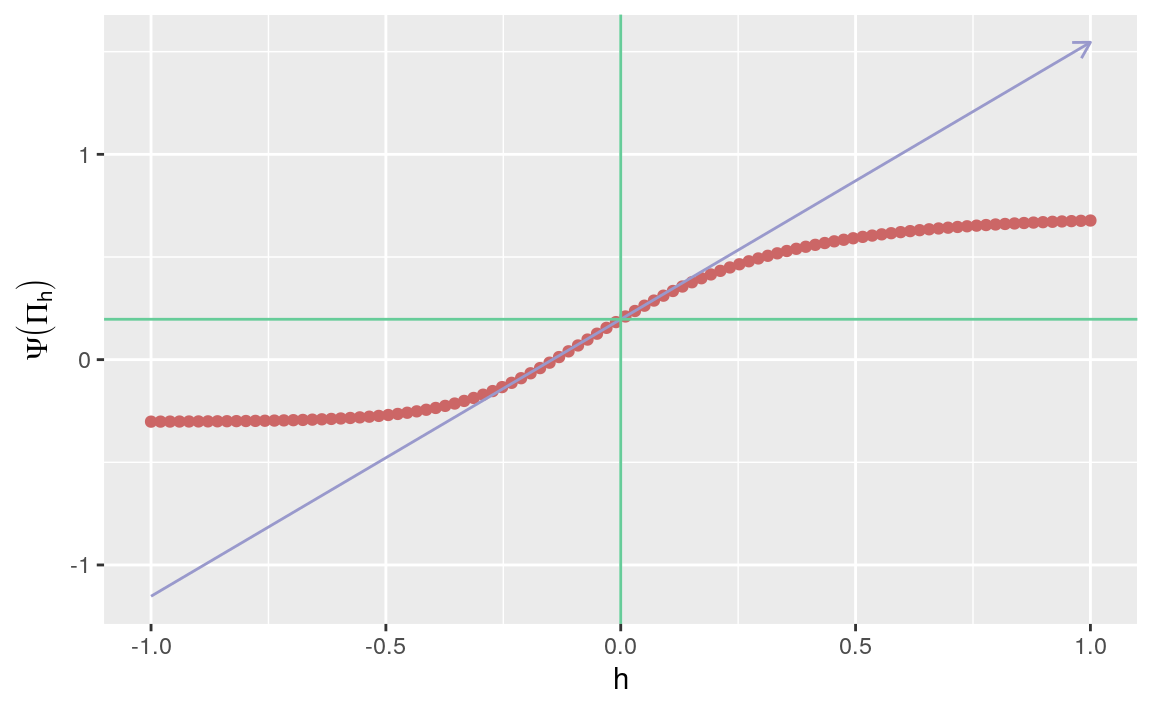
\includegraphics[width=0.7\linewidth]{img/psi-approx-psi-one-1} 

}

\caption{Evolution of statistical mapping \(\Psi\) along fluctuation \(\{\Pi_{h} : h \in H\}\).}\label{fig:psi-approx-psi-one}
\end{figure}

The red curve represents the function \(h \mapsto \Psi(\Pi_{h})\). The blue line
represents the tangent to the previous curve at \(h=0\), which indeed appears to
be differentiable around \(h=0\). In Section \ref{revisiting}, we derive a
closed-form expression for the slope of the blue curve.

\hypertarget{exo-yet-another-experiment}{%
\section{\texorpdfstring{⚙ \gear Yet another experiment}{⚙ Yet another experiment}}\label{exo-yet-another-experiment}}

\begin{enumerate}
\def\labelenumi{\arabic{enumi}.}
\item
  Adapt the code from Problem 1 in Section \ref{exo-visualization} to
  visualize \(w \mapsto \Exp_{\Pi_h}(Y | A = 1, W = w)\), \(w \mapsto \Exp_{\Pi_h}(Y | A = 0, W=w)\), and \(w \mapsto \Exp_{\Pi_h}(Y | A = 1, W=w) - \Exp_{\Pi_h}(Y | A = 0, W=w)\), for \(h \in \{-1/2, 0, 1/2\}\).
\item
  Run the following chunk of code.
\end{enumerate}

\begin{Shaded}
\begin{Highlighting}[]
\NormalTok{yet\_another\_experiment }\OtherTok{\textless{}{-}} \FunctionTok{copy}\NormalTok{(another\_experiment)}
\FunctionTok{alter}\NormalTok{(yet\_another\_experiment,}
      \AttributeTok{Qbar =} \ControlFlowTok{function}\NormalTok{(AW, h)\{}
\NormalTok{        A }\OtherTok{\textless{}{-}}\NormalTok{ AW[, }\StringTok{"A"}\NormalTok{]}
\NormalTok{        W }\OtherTok{\textless{}{-}}\NormalTok{ AW[, }\StringTok{"W"}\NormalTok{]}
        \FunctionTok{expit}\NormalTok{( }\FunctionTok{logit}\NormalTok{( A }\SpecialCharTok{*}\NormalTok{ W }\SpecialCharTok{+}\NormalTok{ (}\DecValTok{1} \SpecialCharTok{{-}}\NormalTok{ A) }\SpecialCharTok{*}\NormalTok{ W}\SpecialCharTok{\^{}}\DecValTok{2}\NormalTok{ ) }\SpecialCharTok{+} 
\NormalTok{               h }\SpecialCharTok{*}\NormalTok{ (}\DecValTok{2}\SpecialCharTok{*}\NormalTok{A }\SpecialCharTok{{-}} \DecValTok{1}\NormalTok{) }\SpecialCharTok{/} \FunctionTok{ifelse}\NormalTok{(A }\SpecialCharTok{==} \DecValTok{1}\NormalTok{,}
                                      \FunctionTok{sin}\NormalTok{((}\DecValTok{1} \SpecialCharTok{+}\NormalTok{ W) }\SpecialCharTok{*}\NormalTok{ pi }\SpecialCharTok{/} \DecValTok{6}\NormalTok{), }
                                      \DecValTok{1} \SpecialCharTok{{-}} \FunctionTok{sin}\NormalTok{((}\DecValTok{1} \SpecialCharTok{+}\NormalTok{ W) }\SpecialCharTok{*}\NormalTok{ pi }\SpecialCharTok{/} \DecValTok{6}\NormalTok{)) }\SpecialCharTok{*}
\NormalTok{               (Y }\SpecialCharTok{{-}}\NormalTok{ A }\SpecialCharTok{*}\NormalTok{ W }\SpecialCharTok{+}\NormalTok{ (}\DecValTok{1} \SpecialCharTok{{-}}\NormalTok{ A) }\SpecialCharTok{*}\NormalTok{ W}\SpecialCharTok{\^{}}\DecValTok{2}\NormalTok{))}
\NormalTok{      \})}
\end{Highlighting}
\end{Shaded}

\begin{enumerate}
\def\labelenumi{\arabic{enumi}.}
\setcounter{enumi}{2}
\item
  Justify that \texttt{yet\_another\_fluctuation} characterizes another fluctuation of
  \(\Pi_{0}\). Comment upon the similarities and differences between \(\{\Pi_{h} : h \in ]-1,1[\}\) and \(\{\Pi_{h}' : h \in ]-1,1[\}\).
\item
  Repeat Problem 1 above with \(\Pi_{h}'\) substituted for \(\Pi_{h}\).
\item
  Re-produce Figure \ref{fig:psi-approx-psi-one} for the \(\{\Pi_h' : h \in ]-1,1[\}\) fluctuation. Comment on the similarities and differences between
  the resulting figure and Figure \ref{fig:psi-approx-psi-one}. In particular,
  how does the behavior of the target parameter around \(h = 0\) compare between
  laws \(\Pi_0\) and \(\Pi_0'\)?
\end{enumerate}

\hypertarget{smooth-second-pass}{%
\section{\texorpdfstring{☡ \stixdanger{} More on fluctuations and smoothness}{☡  More on fluctuations and smoothness}}\label{smooth-second-pass}}

\hypertarget{smooth-second-pass-fluctuations}{%
\subsection{Fluctuations}\label{smooth-second-pass-fluctuations}}

Let us now formally define what it means for statistical mapping \(\Psi\) to be
smooth at every \(P \in \calM\). Let \(H\) be the interval \(]-1/M,M[\). For every
\(h \in H\), we can define a law \(P_{h} \in \calM\) by setting \(P_{h} \ll P\)\footnote{That is, \(P_{h}\) is dominated by \(P\): if an event \(A\) satisfies \(P(A) = 0\), then necessarily \(P_{h} (A) = 0\) too. Because \(P_{h} \ll P\), the law
  \(P_{h}\) has a density with respect to \(P\), meaning that there exists a
  (measurable) function \(f\) such that \(P_{h}(A) = \int_{o \in A} f(o) dP(o)\) for
  any event \(A\). The function is often denoted \(dP_{h}/dP\).} and
\begin{equation} \frac{dP_h}{dP} \defq 1 + h s, 
\label{eq:fluct} \end{equation}
where \(s : \calO\to \bbR\) is a (measurable) function of \(O\) such that \(s(O)\)
is not equal to zero \(P\)-almost surely, \(\Exp_{P} (s(O)) = 0\), and \(s\) bounded
by \(M\). We make the observation that
\begin{equation} (i) \quad P_h|_{h=0} =
P,\quad  (ii)  \quad \left.\frac{d}{dh}  \log  \frac{dP_h}{dP}(O)\right|_{h=0}
=s(O).  \label{eq:score} 
\end{equation}

Because of \emph{(i)}, \(\{P_{h} : h \in H\}\) is a submodel through \(P\), also
referred to as a \emph{fluctuation} of \(P\). The fluctuation is a one-dimensional
submodel of \(\calM\) with univariate parameter \(h \in H\). We note that \emph{(ii)}
indicates that the score of this submodel at \(h = 0\) is \(s\). Thus, we say
that the fluctuation is \emph{in the direction} of \(s\).

Fluctuations of \(P\) do not necessarily take the same form as in
\eqref{eq:fluct}. No matter how the fluctuation is built, for our purposes the
most important feature of the fluctuation is its direction.

\hypertarget{smoothness-and-gradients}{%
\subsection{Smoothness and gradients}\label{smoothness-and-gradients}}

We are now prepared to provide a formal definition of smoothness of
statistical mappings. We say that a statistical mapping \(\Psi\) is \emph{smooth} at
every \(P \in \calM\) if for each \(P \in \calM\), there exists a (measurable)
function \(D^{*}(P) : \calO \to \bbR\) such that \(\Exp_{P}(D^{*}(P)(O)) = 0\),
\(\Var_{P}(D^{*}(P)(O)) < \infty\), and, for every fluctuation \(\{P_{h} : h \in H\}\) with score \(s\) at \(h = 0\), the real-valued mapping \(h \mapsto \Psi(P_{h})\) is differentiable at \(h=0\), with a derivative equal to
\begin{equation} 
\Exp_{P} \left( D^{*}(P)(O) s(O) \right).  \label{eq:derivative} 
\end{equation}
The object \(D^*(P)\) in \eqref{eq:derivative} is called a
gradient of \(\Psi\) at \(P\).\footnote{Interestingly, if a fluctuation \(\{P_{h} : h \in H\}\) satisfies \eqref{eq:score} for a direction \(s\) such that \(s\neq 0\),
  \(\Exp_{P}(s(O)) = 0\) and \(\Var_{P} (s(O)) < \infty\), then \(h \mapsto \Psi(P_{h})\) is still differentiable at \(h=0\) with a derivative equal to
  \eqref{eq:derivative} beyond fluctuations of the form \eqref{eq:fluct}.}

\hypertarget{Euclidean-perspective}{%
\subsection{A Euclidean perspective}\label{Euclidean-perspective}}

This terminology has a direct parallel to directional derivatives in the
calculus of Euclidean geometry. Recall that if \(f\) is a differentiable
mapping from \(\bbR^p\) to \(\bbR\), then the directional derivative of \(f\) at \emph{a
point} \(x\) (an element of \(\bbR^p\)) in \emph{direction} \(u\) (a unit vector in
\(\bbR^p\)) is the scalar product of the gradient of \(f\) and \(u\). In words, the
directional derivative of \(f\) at \(x\) can be represented as a scalar product of
the direction that we approach \(x\) and the change of the function's value at
\(x\).

In the present problem, the law \(P\) is \emph{the point} at which we evaluate the
function \(\Psi\), the score \(s\) of the fluctuation is \emph{the direction} in which
we approach the point, and the gradient describes the change in the function's
value at the point.

\hypertarget{canonical-gradient}{%
\subsection{The canonical gradient}\label{canonical-gradient}}

In general, it is possible for many gradients to exist\footnote{This may be at first
  surprising given the parallel drawn in Section \ref{Euclidean-perspective} to
  Euclidean geometry. However, it is important to remember that the model
  dictates fluctuations of \(P\) that are valid submodels with respect to the full
  model. In turn, this determines the possible directions from which we may
  approach \(P\). Thus, depending on the direction, \eqref{eq:derivative} may hold
  with different choices of \(D^*\).}. Yet, in the special case that the model is
nonparametric, only a single gradient exists. The unique gradient is then
referred to as \emph{the canonical gradient} or,
for reasons that will be clarified in Section \ref{influence-curves}, \emph{the efficient influence curve}. In the
more general setting, the canonical gradient may be defined as the minimizer
of \(D\mapsto \Var_{P} (D(O))\) over the set of all gradients of \(\Psi\) at \(P\).

It is not difficult to check that the efficient influence curve of statistical
mapping \(\Psi\) \eqref{eq:psimap} at \(P \in \calM\) can be written as
\begin{align}  D^{*}(P)  &  \defq  D_{1}^{*}   (P)  +  D_{2}^{*}  (P),  \quad
\text{where} \label{eq:eif}\\  D_{1}^{*}(P) (O) &\defq \Qbar(1,W)  - \Qbar(0,W) -
\Psi(P),  \notag\\ D_{2}^{*}(P)  (O)  &\defq \frac{2A-1}{\ell\Gbar(A,W)}(Y  -
\Qbar(A,W)).\notag \end{align}

A \texttt{method} from package \texttt{tlrider} evaluates the efficient influence curve at a
law described by an object of class \texttt{LAW}. It is called \texttt{evaluate\_eic}. For
instance, the next chunk of code evaluates the efficient influence curve
\(D^{*}(P_{0})\) of \(\Psi\) \eqref{eq:psimap} at \(P_{0} \in \calM\) that is
characterized by \texttt{experiment}:

\begin{Shaded}
\begin{Highlighting}[]
\NormalTok{eic\_experiment }\OtherTok{\textless{}{-}} \FunctionTok{evaluate\_eic}\NormalTok{(experiment)}
\end{Highlighting}
\end{Shaded}

The efficient influence curve \(D^{*}(P_{0})\) is a function from \(\calO\) to
\(\bbR\). As such, it can be evaluated at the five independent observations
drawn from \(P_{0}\) in Section \ref{synthetic-experiment}. This is what the
next chunk of code does:

\begin{Shaded}
\begin{Highlighting}[]
\NormalTok{(}\FunctionTok{eic\_experiment}\NormalTok{(five\_obs))}
\CommentTok{\#\textgreater{} [1] {-}0.0241 {-}0.0283  0.1829  0.0374 {-}0.0463}
\end{Highlighting}
\end{Shaded}

Finally, the efficient influence curve can be visualized as two images that
represent \((w,y) \mapsto D^{*}(P_{0})(w,a,y)\) for \(a = 0,1\), respectively:



\begin{Shaded}
\begin{Highlighting}[]
\FunctionTok{crossing}\NormalTok{(}\AttributeTok{w =} \FunctionTok{seq}\NormalTok{(}\DecValTok{0}\NormalTok{, }\DecValTok{1}\NormalTok{, }\AttributeTok{length.out =} \FloatTok{2e2}\NormalTok{),}
     \AttributeTok{a =} \FunctionTok{c}\NormalTok{(}\DecValTok{0}\NormalTok{, }\DecValTok{1}\NormalTok{),}
     \AttributeTok{y =} \FunctionTok{seq}\NormalTok{(}\DecValTok{0}\NormalTok{, }\DecValTok{1}\NormalTok{, }\AttributeTok{length.out =} \FloatTok{2e2}\NormalTok{)) }\SpecialCharTok{\%\textgreater{}\%}
  \FunctionTok{mutate}\NormalTok{(}\AttributeTok{eic =} \FunctionTok{eic\_experiment}\NormalTok{(}\FunctionTok{cbind}\NormalTok{(}\AttributeTok{Y=}\NormalTok{y,}\AttributeTok{A=}\NormalTok{a,}\AttributeTok{W=}\NormalTok{w))) }\SpecialCharTok{\%\textgreater{}\%}
  \FunctionTok{ggplot}\NormalTok{(}\FunctionTok{aes}\NormalTok{(}\AttributeTok{x =}\NormalTok{ w, }\AttributeTok{y =}\NormalTok{ y, }\AttributeTok{fill =}\NormalTok{ eic)) }\SpecialCharTok{+}
  \FunctionTok{geom\_raster}\NormalTok{(}\AttributeTok{interpolate =} \ConstantTok{TRUE}\NormalTok{) }\SpecialCharTok{+}
  \FunctionTok{geom\_contour}\NormalTok{(}\FunctionTok{aes}\NormalTok{(}\AttributeTok{z =}\NormalTok{ eic), }\AttributeTok{color =} \StringTok{"white"}\NormalTok{) }\SpecialCharTok{+}
  \FunctionTok{facet\_wrap}\NormalTok{(}\SpecialCharTok{\textasciitilde{}}\NormalTok{ a, }\AttributeTok{nrow =} \DecValTok{1}\NormalTok{,}
             \AttributeTok{labeller =} \FunctionTok{as\_labeller}\NormalTok{(}\FunctionTok{c}\NormalTok{(}\StringTok{\textasciigrave{}}\AttributeTok{0}\StringTok{\textasciigrave{}} \OtherTok{=} \StringTok{"a = 0"}\NormalTok{, }\StringTok{\textasciigrave{}}\AttributeTok{1}\StringTok{\textasciigrave{}} \OtherTok{=} \StringTok{"a = 1"}\NormalTok{))) }\SpecialCharTok{+}
  \FunctionTok{labs}\NormalTok{(}\AttributeTok{fill =} \FunctionTok{expression}\NormalTok{(}\FunctionTok{paste}\NormalTok{(D}\SpecialCharTok{\^{}}\StringTok{"*"}\NormalTok{, (P[}\DecValTok{0}\NormalTok{])(w,a,y))))}
\end{Highlighting}
\end{Shaded}

\begin{figure}

{\centering 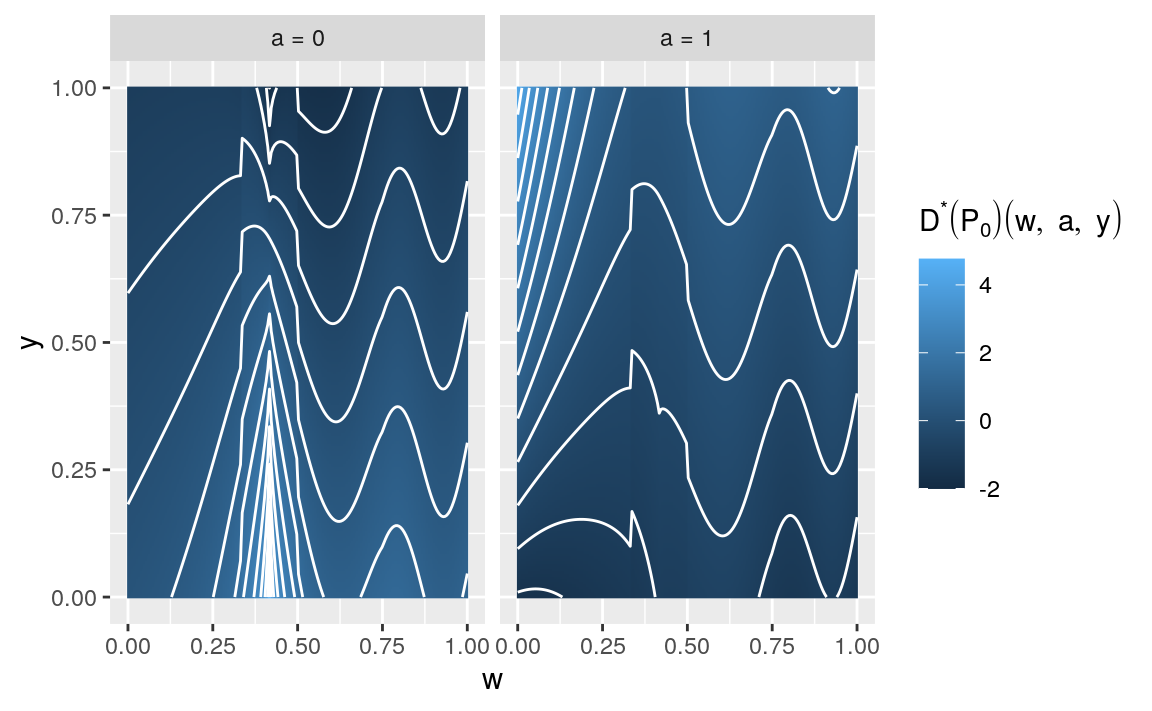
\includegraphics[width=0.8\linewidth]{img/eic-three-1} 

}

\caption{Visualizing the efficient influence curve \(D^{*}(P_{0})\) of \(\Psi\) \eqref{eq:psimap} at \(P_{0}\), the law described by \texttt{experiment}.}\label{fig:eic-three}
\end{figure}

\hypertarget{revisiting}{%
\section{\texorpdfstring{A fresh look at \texttt{another\_experiment}}{A fresh look at another\_experiment}}\label{revisiting}}

We can give a fresh look at Section \ref{numerical-illus} now.

\hypertarget{deriving-the-efficient-influence-curve}{%
\subsection{Deriving the efficient influence curve}\label{deriving-the-efficient-influence-curve}}

It is not difficult (though cumbersome) to verify that, up to a constant,
\(\{\Pi_{h} : h \in [-1,1]\}\) is a fluctuation of \(\Pi_{0}\) in the direction
(in the sense of \eqref{eq:fluct}) of

\begin{align}
\notag\sigma_{0}(O)  \defq &- 10 \sqrt{W} A \times \beta_{0}  (A,W)\\
&\times\left(\log(1    -     Y)    +     \sum_{k=0}^{3}    \left(k     +    \beta_{0}
(A,W)\right)^{-1}\right) + \text{constant}, \quad \text{where}\\
\beta_{0}(A,W)\defq & \frac{1
-\Qbar_{\Pi_{0}}(A,W)}{\Qbar_{\Pi_{0}}(A,W)}. \label{eq:sigma0}\end{align}

Consequently, the slope of line in Figure \ref{fig:psi-approx-psi-one} is
equal to

\begin{equation}
\Exp_{\Pi_{0}} (D^{*}(\Pi_{0}) (O) \sigma_{0}(O)). \label{eq:slope-Pi}
\end{equation}

Since \(D^{*}(\Pi_{0})\) is centered under \(\Pi_{0}\), knowing \(\sigma_{0}\) up
to a constant is not problematic.

\hypertarget{numerical-validation}{%
\subsection{Numerical validation}\label{numerical-validation}}

In the following code, we check the above fact numerically. When we ran
\texttt{example(tlrider)}, we created a function \texttt{sigma0}. The function implements
\(\sigma_{0}\) defined in \eqref{eq:sigma0}:

\begin{Shaded}
\begin{Highlighting}[]
\NormalTok{sigma0}
\CommentTok{\#\textgreater{} function(obs, law = another\_experiment) \{}
\CommentTok{\#\textgreater{}   \#\# preliminary}
\CommentTok{\#\textgreater{}   Qbar \textless{}{-} get\_feature(law, "Qbar", h = 0)}
\CommentTok{\#\textgreater{}   QAW \textless{}{-} Qbar(obs[, c("A", "W")])}
\CommentTok{\#\textgreater{}   params \textless{}{-} formals(get\_feature(law, "qY", h = 0))}
\CommentTok{\#\textgreater{}   shape1 \textless{}{-} eval(params$shape1)}
\CommentTok{\#\textgreater{}   \#\# computations}
\CommentTok{\#\textgreater{}   betaAW \textless{}{-} shape1 * (1 {-} QAW) / QAW}
\CommentTok{\#\textgreater{}   out \textless{}{-} log(1 {-} obs[, "Y"])}
\CommentTok{\#\textgreater{}   for (int in 1:shape1) \{}
\CommentTok{\#\textgreater{}     out \textless{}{-} out + 1/(int {-} 1 + betaAW)}
\CommentTok{\#\textgreater{}   \}}
\CommentTok{\#\textgreater{}   out \textless{}{-} {-} out * shape1 * (1 {-} QAW) / QAW *}
\CommentTok{\#\textgreater{}            10 * sqrt(obs[, "W"]) * obs[, "A"]}
\CommentTok{\#\textgreater{}   \#\# no need to center given how we will use it}
\CommentTok{\#\textgreater{}   return(out)}
\CommentTok{\#\textgreater{}  \}}
\end{Highlighting}
\end{Shaded}

The next chunk of code approximates
\eqref{eq:slope-Pi} pointwise and with a confidence interval of asymptotic
level 95\%:

\begin{Shaded}
\begin{Highlighting}[]
\NormalTok{eic\_another\_experiment }\OtherTok{\textless{}{-}} \FunctionTok{evaluate\_eic}\NormalTok{(another\_experiment, }\AttributeTok{h =} \DecValTok{0}\NormalTok{)}
\NormalTok{obs\_another\_experiment }\OtherTok{\textless{}{-}} \FunctionTok{sample\_from}\NormalTok{(another\_experiment, B, }\AttributeTok{h =} \DecValTok{0}\NormalTok{)}
\NormalTok{vars }\OtherTok{\textless{}{-}} \FunctionTok{eic\_another\_experiment}\NormalTok{(obs\_another\_experiment) }\SpecialCharTok{*}
  \FunctionTok{sigma0}\NormalTok{(obs\_another\_experiment)}

\NormalTok{sd\_hat }\OtherTok{\textless{}{-}} \FunctionTok{sd}\NormalTok{(vars)}
\NormalTok{(slope\_hat }\OtherTok{\textless{}{-}} \FunctionTok{mean}\NormalTok{(vars))}
\CommentTok{\#\textgreater{} [1] 1.35}
\NormalTok{(slope\_CI }\OtherTok{\textless{}{-}}\NormalTok{ slope\_hat }\SpecialCharTok{+} \FunctionTok{c}\NormalTok{(}\SpecialCharTok{{-}}\DecValTok{1}\NormalTok{, }\DecValTok{1}\NormalTok{) }\SpecialCharTok{*}
   \FunctionTok{qnorm}\NormalTok{(}\DecValTok{1} \SpecialCharTok{{-}}\NormalTok{ alpha }\SpecialCharTok{/} \DecValTok{2}\NormalTok{) }\SpecialCharTok{*}\NormalTok{ sd\_hat }\SpecialCharTok{/} \FunctionTok{sqrt}\NormalTok{(B))}
\CommentTok{\#\textgreater{} [1] 1.35 1.36}
\end{Highlighting}
\end{Shaded}

Equal to 1.349 (rounded to three decimal places ---
hereafter, all rounding will be to three decimal places as well), the first
numerical approximation \texttt{slope\_approx} is not too off!

\hypertarget{influence-curves}{%
\section{\texorpdfstring{☡ \stixdanger{} Asymptotic linearity and statistical efficiency}{☡  Asymptotic linearity and statistical efficiency}}\label{influence-curves}}

\hypertarget{asymptotic-linearity}{%
\subsection{Asymptotic linearity}\label{asymptotic-linearity}}

Suppose that \(O_{1}, \ldots, O_{n}\) are drawn independently from \(P\in \calM\). If an estimator \(\psi_n\) of \(\Psi(P)\) can be written as

\begin{equation} 
\psi_n  =  \Psi(P) +  \frac{1}{n}\sum_{i=1}^n  \IC(O_i)  +
o_{P}(1/\sqrt{n}) \label{eq:asymptotic-lin}
\end{equation}

for some function \(\IC : \calO \to \bbR\) such that \(\Exp_P(\IC(O)) = 0\) and
\(\Var_{P}(\IC(O)) < \infty\), then we say that \(\psi_n\) is \emph{asymptotically
linear} with \emph{influence curve} \(\IC\). Asymptotically linear estimators are
\emph{weakly convergent}. Specifically, if \(\psi_n\) is asymptotically linear with
influence curve \(\IC\), then

\begin{equation}
\sqrt{n}  (\psi_n  - \Psi(P))  =  \frac{1}{\sqrt{n}}  \sum_{i=1}^n \IC(O_i)  +
o_P(1) \label{eq:asymp-lin}
\end{equation}

and, by the central limit theorem (recall that \(O_{1}, \ldots, O_{n}\) are
independent), \(\sqrt{n} (\psi_n - \Psi(P))\) converges in law to a centered
Gaussian distribution with variance \(\Var_P(\IC(O))\).

\hypertarget{influence-curves-and-gradients}{%
\subsection{Influence curves and gradients}\label{influence-curves-and-gradients}}

As it happens, influence curves of regular\footnote{We can view \(\psi_{n}\) as the by
  product of an algorithm\index{algorithm} \(\Psihat\) trained on independent
  observations \(O_{1}, \ldots, O_{n}\) drawn from \(P\). We say that the estimator
  is regular at \(P\) if, for any direction \(s\neq 0\) such that \(\Exp_{P} (s(O)) = 0\) and \(\Var_{P} (s(O)) < \infty\) and fluctuation \(\{P_{h} : h \in H\}\)
  satisfying \eqref{eq:score}, the estimator \(\psi_{n,1/\sqrt{n}}\) of
  \(\Psi(P_{1/\sqrt{n}})\) obtained by training \(\Psihat\) on independent
  observations \(O_{1}\), \ldots, \(O_{n}\) drawn from \(P_{1/\sqrt{n}}\) is such that
  \(\sqrt{n} (\psi_{n,1/\sqrt{n}} - \Psi(P_{1/\sqrt{n}}))\) converges in law to a
  limit that does not depend on \(s\).} estimators are intimately related to
gradients. In fact, if \(\psi_n\) is a regular, asymptotically linear estimator
of \(\Psi(P)\) with influence curve \(\IC\), then it must be true that \(\Psi\) is a
smooth parameter at \(P\) and that \(\IC\) is a gradient of \(\Psi\) at \(P\).

\hypertarget{asymptotic-efficiency}{%
\subsection{Asymptotic efficiency}\label{asymptotic-efficiency}}

Now recall that, in Section \ref{canonical-gradient}, we defined the
canonical gradient as the minimizer of \(D \mapsto \Var_{P}(D(O))\) over the set
of all gradients. Therefore, if \(\psi_{n}\) is a regular, asymptotically linear
estimator of \(\Psi(P)\) (built from \(n\) independent observations drawn from
\(P\)), then the asymptotic variance of \(\sqrt{n} (\psi_{n} - \Psi(P))\) cannot
be smaller than the variance of the canonical gradient of \(\Psi\) at \(P\),
\emph{i.e.},

\begin{equation}
\label{eq:CR}\Var_{P}(D^{*}(P)(O)). 
\end{equation}

In other words, \eqref{eq:CR} is the lower bound on the asymptotic variance of
\emph{any} regular, asymptotically linear estimator of \(\Psi(P)\). This bound is
referred to as the \emph{Cramér-Rao bound}. Any regular estimator that achieves
this variance bound is said to be \emph{asymptotically efficient} at \(P\). Because
the canonical gradient is the influence curve of an asymptotically efficient
estimator, it is often referred to as the \emph{efficient influence curve}.

\hypertarget{exo-cramer-rao}{%
\section{\texorpdfstring{⚙ \gear Cramér-Rao bounds}{⚙ Cramér-Rao bounds}}\label{exo-cramer-rao}}

\begin{enumerate}
\def\labelenumi{\arabic{enumi}.}
\tightlist
\item
  What does the following chunk do?
\end{enumerate}

\begin{Shaded}
\begin{Highlighting}[]
\NormalTok{obs }\OtherTok{\textless{}{-}} \FunctionTok{sample\_from}\NormalTok{(experiment, B)}
\NormalTok{(cramer\_rao\_hat }\OtherTok{\textless{}{-}} \FunctionTok{var}\NormalTok{(}\FunctionTok{eic\_experiment}\NormalTok{(obs)))}
\CommentTok{\#\textgreater{} [1] 0.287}
\end{Highlighting}
\end{Shaded}

\begin{enumerate}
\def\labelenumi{\arabic{enumi}.}
\setcounter{enumi}{1}
\tightlist
\item
  Same question about this one.
\end{enumerate}

\begin{Shaded}
\begin{Highlighting}[]
\NormalTok{obs\_another\_experiment }\OtherTok{\textless{}{-}} \FunctionTok{sample\_from}\NormalTok{(another\_experiment, B, }\AttributeTok{h =} \DecValTok{0}\NormalTok{)}
\NormalTok{(cramer\_rao\_Pi\_zero\_hat }\OtherTok{\textless{}{-}}
   \FunctionTok{var}\NormalTok{(}\FunctionTok{eic\_another\_experiment}\NormalTok{(obs\_another\_experiment)))}
\CommentTok{\#\textgreater{} [1] 0.0946}
\end{Highlighting}
\end{Shaded}

\begin{enumerate}
\def\labelenumi{\arabic{enumi}.}
\setcounter{enumi}{2}
\item
  With a large independent sample drawn from \(\Psi(P_0)\) (or \(\Psi(\Pi_0)\)),
  is it possible to construct a regular estimator \(\psi_{n}\) of \(\Psi(P_0)\)
  (or \(\Psi(\Pi_0)\)) such that the asymptotic variance of \(\sqrt{n}\) times
  \(\psi_{n}\) minus its target be smaller than the Cramér-Rao bound?
\item
  Is it easier to estimate \(\Psi(P_{0})\) or \(\Psi(\Pi_{0})\) (from independent
  observations drawn from either law)? In what sense? (Hint: you may want to
  compute a ratio.)
\end{enumerate}

\hypertarget{double-robustness}{%
\chapter{Double-robustness}\label{double-robustness}}

\hypertarget{linear-approximation}{%
\section{Linear approximations of parameters}\label{linear-approximation}}

\hypertarget{from-gradients-to-estimators}{%
\subsection{From gradients to estimators}\label{from-gradients-to-estimators}}

We learned in Section \ref{smooth} that the stochastic behavior of a regular,
asymptotically linear estimator of \(\Psi(P)\) can be characterized by its
influence curve. Moreover, we said that this influence curve must in fact be a
gradient of \(\Psi\) at \(P\).

In this section, we show that the converse is also true: given a gradient
\(D^*\) of \(\Psi\) at \(P\), under so-called \emph{regularity conditions}, it is
possible to construct an estimator with influence curve equal to
\(D^*(P)\). This fact will suggest concrete strategies for generating efficient
estimators of smooth parameters. We take here the first step towards
generating such estimators: linearizing the parameter.

\hypertarget{another-Euclidean-perspective}{%
\subsection{A Euclidean perspective}\label{another-Euclidean-perspective}}

As in Section \ref{Euclidean-perspective}, drawing a parallel to Euclidean
geometry is helpful. We recall that if \(f\) is a differentiable mapping from
\(\bbR^p\) to \(\bbR\), then a Taylor series approximates \(f\) at a point \(x_0 \in \bbR^p\): \begin{equation*} f(x_0)  \approx f(x)  + \langle(x_0  - x),  \nabla
f(x)\rangle,\end{equation*} where \(x\) is a point in \(\bbR^p\), \(\nabla f(x)\) is
the gradient of \(f\) evaluated at \(x\) and \(\langle u,v\rangle\) is the scalar
product of \(u,v \in \bbR^{p}\). As the squared distance \(\|x-x_{0}\|^{2} = \langle x-x_{0}, x-x_{0}\rangle\) between \(x\) and \(x_0\) decreases, the \emph{linear
approximation} to \(f(x_0)\) becomes more accurate.

\hypertarget{the-remainder-term}{%
\subsection{The remainder term}\label{the-remainder-term}}

Returning to the present problem with this in mind, we find that indeed a
similar approximation strategy may be applied.

For clarity, let us introduce a new shorthand notation. For any measurable
function \(f\) of the observed data \(O\), we may write from now on \(P f \defq \Exp_P(f(O))\). One may argue that the notation is valuable beyond the gain of
space. For instance, \eqref{eq:asymp-lin}

\begin{equation*}
\sqrt{n}  (\psi_n  - \Psi(P))  =  \frac{1}{\sqrt{n}}  \sum_{i=1}^n \IC(O_i)  +
o_P(1) 
\end{equation*}

can be rewritten as

\begin{equation*}
\sqrt{n} (\psi_n - \Psi(P)) = \sqrt{n} (P_{n} - P) \IC + o_P(1),
\end{equation*}

thus suggesting more clearly the importance of the so-called \emph{empirical
process} \(\sqrt{n} (P_{n} - P)\).

In particular, if \(\Psi\) is smooth uniformly over directions, then for any
given \(P \in \calM\), we can write

\begin{equation} 
\Psi(P_0)    =   \Psi(P)    +   (P_0    -   P)    D^*(P)   -    \Rem_{P_0}(P),
\label{eq:taylor-expansion} 
\end{equation}

where \(\Rem_{P_0}(P)\) (defined \emph{implicitly} by \eqref{eq:taylor-expansion} --
see \eqref{eq:remainder-one}) is a
\emph{remainder term} satisfying that \begin{equation*} \frac{\Rem_{P_0}(P)}{d(P,
P_0)} \rightarrow  0 \ \mbox{as} \  d(P, P_0) \rightarrow 0  , \end{equation*}
with \(d\) a measure of discrepancy for distributions in \(\calM\). Note that
\eqref{eq:taylor-expansion} can be equivalently written as \begin{equation*}
\Psi(P_0)   =   \Psi(P)   +  \Exp_{P_0}(D^*(P)(O))   -   \Exp_P(D^*(P)(O))   -
\Rem_{P_0}(P).  \end{equation*} The remainder term formalizes the notion that
if \(P\) is \emph{close} to \(P_0\) (\emph{i.e.}, if \(d(P,P_0)\) is small), then the linear
approximation of \(\Psi(P_0)\) is more accurate. In light of
the Euclidean perspective of Section \ref{another-Euclidean-perspective}, the
remainder term \(\Rem_{P_0}(P)\) plays the role of the squared distance \(\|x-x_0\|^{2}\).

\hypertarget{expressing-the-remainder-term-as-a-function-of-the-relevant-features}{%
\subsection{Expressing the remainder term as a function of the relevant features}\label{expressing-the-remainder-term-as-a-function-of-the-relevant-features}}

The equations for the definition of the parameter \eqref{eq:psimap}, form of
the canonical gradient \eqref{eq:eif}, and linearization of parameter
\eqref{eq:taylor-expansion} combine to determine the remainder:

\begin{equation}
\Rem_{P_0}(P)    \defq   \Psi(P)    -   \Psi(P_0)    -   (P_0    -   P)D^*(P)
\label{eq:remainder-one}
\end{equation}

hence

\begin{multline} 
\Rem_{P_0}(P)=   \Exp_{P_0}   \Bigg[   \left(\Gbar_0(W)   -
\Gbar(W)\right) \\          \times          \left(\frac{\Qbar_0(1,W)           -
\Qbar(1,W)}{\ell\Gbar(1,W)} + \frac{\Qbar_0(0,W) - \Qbar(0,W)}{\ell\Gbar(0,W)}
\right) \Bigg]. \label{eq:remainder} 
\end{multline}

Acting as oracles, we can compute explicitly the remainder term
\(\Rem_{P_0}(P)\). The \texttt{evaluate\_remainder} method makes it very easy (simply
run \texttt{?evaluate\_remainder} to see the man page of the method):

\begin{Shaded}
\begin{Highlighting}[]
\NormalTok{(}\FunctionTok{evaluate\_remainder}\NormalTok{(experiment, experiment))}
\CommentTok{\#\textgreater{} [1] 0}
\NormalTok{(rem }\OtherTok{\textless{}{-}} \FunctionTok{evaluate\_remainder}\NormalTok{(experiment, another\_experiment,}
                           \FunctionTok{list}\NormalTok{(}\FunctionTok{list}\NormalTok{(), }\FunctionTok{list}\NormalTok{(}\AttributeTok{h =} \DecValTok{0}\NormalTok{))))}
\CommentTok{\#\textgreater{} [1] 0.199}
\end{Highlighting}
\end{Shaded}

We recover the equality \(\Rem_{P_{0}} (P_{0}) = 0\), which is fairly obvious
given \eqref{eq:taylor-expansion}. In addition, we learn that \(\Rem_{P_{0}} (\Pi_{0})\) equals 0.199. In the next subsection, we invite you to
make better acquaintance with the remainder term by playing around with it
numerically.

\hypertarget{exo-remainder-term}{%
\section{\texorpdfstring{⚙ \gear The remainder term}{⚙ The remainder term}}\label{exo-remainder-term}}

\begin{enumerate}
\def\labelenumi{\arabic{enumi}.}
\item
  Compute numerically \(\Rem_{\Pi_0}(\Pi_h)\) for \(h \in [-1,1]\) and plot your
  results. What do you notice?
\item
  ☡ \stixdanger{} Approximate \(\Rem_{P_{0}} (\Pi_{0})\) numerically
  without relying on method \texttt{evaluate\_remainder} and compare the value you get
  with that of \texttt{rem}. (Hint: use \eqref{eq:remainder-one} and a large sample of
  observations drawn independently from \(P_{0}\).)
\end{enumerate}

\hypertarget{def-double-robustness}{%
\section{\texorpdfstring{☡ \stixdanger{} Double-robustness}{☡  Double-robustness}}\label{def-double-robustness}}

\hypertarget{the-key-property}{%
\subsection{The key property}\label{the-key-property}}

Let us denote by \(\|f\|_{P}^{2}\) the square of the \(L^{2}(P)\)-norm of any
function \(f\) from \(\calO\) to \(\bbR\) \emph{i.e.}, using a recently introduced
notation, \(\|f\|_{P}^{2} \defq Pf^{2}\). For instance, \(\|\Qbar_{1} - \Qbar_{0}\|_{P}\) or \(\|\Gbar_{1} - \Gbar_{0}\|_{P}\) is a distance separating
the features \(\Qbar_{1}\) and \(\Qbar_{0}\) or \(\Gbar_{1}\) and \(\Gbar_{0}\).

The efficient influence curve \(D^{*}(P)\) at \(P \in \calM\) enjoys a rather
remarkable property: it is \emph{double-robust}. Specifically, for every \(P \in \calM\), the remainder term \(\Rem_{P_{0}} (P)\) satisfies

\begin{equation} 
\Rem_{P_{0}}   (P)^{2}  \leq   \|\Qbar   -
\Qbar_{0}\|_{P_0}^{2}  \times   \|(\Gbar  -  \Gbar_{0})/\ell\Gbar_{0}\|_{P_0}^{2},
\label{eq:rem-two}
\end{equation}

where \(\Qbar\) and \(\Gbar\) are the counterparts under \(P\) to \(\Qbar_{0}\) and
\(\Gbar_{0}\). The proof consists in a straightforward application of the
Cauchy-Schwarz inequality to the right-hand side expression in
\eqref{eq:remainder-one}.

\hypertarget{direct-consequence}{%
\subsection{Its direct consequence}\label{direct-consequence}}

It may not be clear yet why \eqref{eq:rem-two} is an important property, and
why \(D^{*}\) is said \emph{double-robust} because of it. To answer the latter
question, let us consider a law \(P\in \calM\) such that \emph{either} \(\Qbar = \Qbar_{0}\) \emph{or} \(\Gbar = \Gbar_{0}\).

It is then the case that \emph{either} \(\|\Qbar - \Qbar_{0}\|_{P} = 0\) \emph{or}
\(\|\Gbar - \Gbar_{0}\|_{P} = 0\). Therefore, in light of \eqref{eq:rem-two}, it
also holds that \(\Rem_{P_{0}} (P) = 0\).\footnote{This also trivially follows from
  \eqref{eq:remainder}.} It thus appears that \eqref{eq:taylor-expansion}
simplifies to

\begin{align*} \Psi(P_0) &= \Psi(P) + (P_0 - P) D^*(P)\\
&= \Psi(P) + P_0 D^*(P),\end{align*}

where the second equality holds because \(PD^{*}(P) = 0\) for all \(P\in \calM\)
by definition of \(D^{*}(P)\).

It is now clear that for such a law \(P\in \calM\), \(\Psi(P) = \Psi(P_{0})\) is
equivalent to

\begin{equation} 
P_{0} D^{*}(P) = 0. \label{eq:solves-eic} 
\end{equation}

Most importantly, in words, if \(P\) solves the so-called \(P_{0}\)-specific
efficient influence curve equation \eqref{eq:solves-eic} and if, in addition,
\(P\) has the same \(\Qbar\)-feature \emph{or} \(\Gbar\)-feature as \(P_{0}\), then
\(\Psi(P) = \Psi(P_{0})\).

The conclusion is valid no matter how \(P\) may differ from \(P_{0}\) otherwise,
hence the notion of being \emph{double-robust}. This property is useful to build
consistent estimators of \(\Psi(P)\), as we shall see in Section
\ref{inference}.

\hypertarget{exo-double-robustness}{%
\section{\texorpdfstring{⚙ \gear Double-robustness}{⚙ Double-robustness}}\label{exo-double-robustness}}

\begin{enumerate}
\def\labelenumi{\arabic{enumi}.}
\item
  Go back to Problem 1 in \ref{exo-remainder-term}. In light of Section
  \ref{def-double-robustness}, what is happening?
\item
  Create a copy of \texttt{experiment} and replace its \texttt{Gbar} feature with some
  other function of \(W\) (see \texttt{?copy}, \texttt{?alter} and Problem 2 in Section
  \ref{exo-yet-another-experiment}). Call \(P'\) the element of model \(\calM\)
  thus characterized. Can you guess the values of \(\Rem_{P_{0}}(P')\),
  \(\Psi(P')\) and \(P_{0} D^{*}(P')\)? Support your argument.
\end{enumerate}

\hypertarget{inference}{%
\chapter{Inference}\label{inference}}

\hypertarget{where-we-stand}{%
\section{Where we stand}\label{where-we-stand}}

In the previous sections, we analyzed our target parameter and presented
relevant theory for understanding the statistical properties of certain types
of estimators of the parameter. The theory is also relevant for building and
comparing a variety of estimators.

We assume from now on that we have available a sample \(O_{1}, \ldots, O_{B}\)
of independent observations drawn from \(P_{0}\). This is literally the case!,
and the observations are stored in \texttt{obs} that we created in Section
\ref{exo-cramer-rao}.

\begin{Shaded}
\begin{Highlighting}[]
\NormalTok{iter }\OtherTok{\textless{}{-}} \FloatTok{1e3}
\end{Highlighting}
\end{Shaded}

Equal to 1000 thousands, the sample size \texttt{B} is very large. We will in
fact use 1000 disjoint subsamples composed of \(n\) independent
observations among \(O_{1}, \ldots, O_{B}\), where \(n\) equals \texttt{B/iter}, \emph{i.e.},
1000. We will thus be in a position to investigate the
statistical properties of every estimation procedure by replicating it
independently 1000 times.

\hypertarget{where-we-are-going}{%
\section{Where we are going}\label{where-we-are-going}}

The following sections explore different statistical paths to inferring
\(\psi_{0}\) or, rather (though equivalently), \(\Psi(P_{0})\).

\begin{itemize}
\item
  Section \ref{simple-strategy} presents a simple inference strategy. It can
  be carried out in situations where \(\Gbar_{0}\) is already known to the
  statistician.
\item
  Section \ref{nuisance} discusses the estimation of some
  infinite-dimensional features of \(P_{0}\). The resulting estimators are
  later used to estimate \(\psi_{0}\).
\item
  Section \ref{naive-estimators} extends the inference strategy discussed in
  Section \ref{simple-strategy} to the case that \(\Gbar_{0}\) is not known to
  the statistician but estimated by her. It also presents another inference
  strategy that relies upon the estimation of \(\Qbar_{0}\). A theoretical
  analysis reveals that both strategies, called the \emph{inverse probability of
  treatment weighted} and \emph{G-computation} estimation methodologies, suffer
  from an inherent flaw.
\item
  Section \ref{one-step} builds upon the aforementioned analysis and develops
  a methodological workaround to circumvent the problem revealed by the
  analysis. It appears indeed that the flawed estimators can be
  corrected. However, the so-called \emph{one-step correction} comes at a price
  that may be high in small samples.
\item
  Section \ref{TMLE} also builds on the aforementioned analysis but draws a
  radically different conclusion from it. Instead of trying to circumvent the
  problem by correcting the flawed estimators of \(\psi_{0}\), it does so by
  correcting the estimators of the infinite-dimensional features of \(P_{0}\)
  combined to estimate \(\psi_{0}\). The section thus presents an instantiation
  of the general \emph{targeted minimum loss estimation} procedure tailored to the
  estimation of \(\psi_{0}\). It is the main destination of this ride in
  targeted learning territory, far from its outposts yet well into this
  exciting territory.
\end{itemize}

\hypertarget{simple-strategy}{%
\chapter{A simple inference strategy}\label{simple-strategy}}

\hypertarget{a-cautionary-detour}{%
\section{A cautionary detour}\label{a-cautionary-detour}}

Let us introduce first the following estimator:

\begin{align}
\notag \psi_{n}^{a}
&\defq \frac{\Exp_{P_{n}} (AY)}{\Exp_{P_{n}} (A)} - \frac{\Exp_{P_{n}}
((1-A)Y)}{\Exp_{P_{n}}(1-A)} \\ 
&=          \frac{\sum_{i=1}^{n}         \one\{A_{i}=Y_{i}=1\}}{\sum_{i=1}^{n}
\one\{A_{i}=1\}}                     -                    \frac{\sum_{i=1}^{n}
\one\{A_{i}=0,Y_{i}=1\}}{\sum_{i=1}^{n}\one\{A_{i}=0\}}. \label{eq:cautionary} 
\end{align}

Note that \(\psi_n^a\) is simply the difference in sample means between
observations with \(A = 1\) and observations with \(A = 0\). It estimates
\begin{align*}\Phi(P_{0}) &\defq \frac{\Exp_{P_{0}}
(AY)}{\Exp_{P_{0}} (A)} - \frac{\Exp_{P_{0}} ((1-A)Y)}{\Exp_{P_{0}} (1-A)}\\&=
\Exp_{P_{0}} (Y | A=1) - \Exp_{P_{0}} (Y | A=0).\end{align*}

We seize this opportunity to demonstrate numerically that
\(\psi_{n}^{a}\) \emph{does not} estimate \(\Psi(P_{0})\) because, in general,
\(\Psi(P_{0})\) and \(\Phi(P_{0})\) differ. This is apparent in the following
alternative expression of \(\Phi(P_{0})\):

\begin{align*} \Phi(P_{0}) &= \Exp_{P_{0}} \left(\Exp_{P_0}(Y \mid A, W) |A=1)
\right) -  \Exp_{P_{0}} \left(\Exp_{P_0}(Y \mid  A, W) | A=0\right)\\  &= \int
\Qbar_{0}(1, w) dP_{0,W|A=1}(w) - \int \Qbar_{0}(0, w) dP_{0,W|A=0}(w).
\end{align*}

Contrast the above equalities and \eqref{eq:psi-zero}. In the latter, the
outer integral is against the marginal law of \(W\) under \(P_{0}\). In the
former, the outer integrals are respectively against the conditional laws of
\(W\) given \(A=1\) and \(A=0\) under \(P_{0}\). Thus \(\Psi(P_0)\) and \(\Phi(P_0)\) will
enjoy equality when the conditional laws of \(W\) given \(A = 1\) and \(W\) given
\(A = 0\) both equal the marginal law of \(W\). This can sometimes be
ensured by design, as in an experiment where \(A\) is randomly allocated to
observations, irrespective of \(W\). However, barring this level of experimental
control, in general the naive estimator may lead us astray in our goal of
drawing causal inference.

\hypertarget{delta-method}{%
\section{\texorpdfstring{⚙ \gear Delta-method}{⚙ Delta-method}}\label{delta-method}}

Consider the next chunk of code:

\begin{Shaded}
\begin{Highlighting}[]
\NormalTok{compute\_irrelevant\_estimator }\OtherTok{\textless{}{-}} \ControlFlowTok{function}\NormalTok{(obs) \{}
\NormalTok{  obs }\OtherTok{\textless{}{-}} \FunctionTok{as\_tibble}\NormalTok{(obs)}
\NormalTok{  Y }\OtherTok{\textless{}{-}} \FunctionTok{pull}\NormalTok{(obs, Y)}
\NormalTok{  A }\OtherTok{\textless{}{-}} \FunctionTok{pull}\NormalTok{(obs, A)}
\NormalTok{  psi\_n }\OtherTok{\textless{}{-}} \FunctionTok{mean}\NormalTok{(A }\SpecialCharTok{*}\NormalTok{ Y) }\SpecialCharTok{/} \FunctionTok{mean}\NormalTok{(A) }\SpecialCharTok{{-}} \FunctionTok{mean}\NormalTok{((}\DecValTok{1} \SpecialCharTok{{-}}\NormalTok{ A) }\SpecialCharTok{*}\NormalTok{ Y) }\SpecialCharTok{/} \FunctionTok{mean}\NormalTok{(}\DecValTok{1} \SpecialCharTok{{-}}\NormalTok{ A)}
\NormalTok{  Var\_n }\OtherTok{\textless{}{-}} \FunctionTok{cov}\NormalTok{(}\FunctionTok{cbind}\NormalTok{(A }\SpecialCharTok{*}\NormalTok{ Y, A, (}\DecValTok{1} \SpecialCharTok{{-}}\NormalTok{ A) }\SpecialCharTok{*}\NormalTok{ Y, (}\DecValTok{1} \SpecialCharTok{{-}}\NormalTok{ A)))}
\NormalTok{  phi\_n }\OtherTok{\textless{}{-}} \FunctionTok{c}\NormalTok{(}\DecValTok{1} \SpecialCharTok{/} \FunctionTok{mean}\NormalTok{(A), }\SpecialCharTok{{-}}\FunctionTok{mean}\NormalTok{(A }\SpecialCharTok{*}\NormalTok{ Y) }\SpecialCharTok{/} \FunctionTok{mean}\NormalTok{(A)}\SpecialCharTok{\^{}}\DecValTok{2}\NormalTok{,}
             \SpecialCharTok{{-}}\DecValTok{1} \SpecialCharTok{/} \FunctionTok{mean}\NormalTok{(}\DecValTok{1} \SpecialCharTok{{-}}\NormalTok{ A),}
             \FunctionTok{mean}\NormalTok{((}\DecValTok{1} \SpecialCharTok{{-}}\NormalTok{ A) }\SpecialCharTok{*}\NormalTok{ Y) }\SpecialCharTok{/} \FunctionTok{mean}\NormalTok{(}\DecValTok{1} \SpecialCharTok{{-}}\NormalTok{ A)}\SpecialCharTok{\^{}}\DecValTok{2}\NormalTok{)}
\NormalTok{  var\_n }\OtherTok{\textless{}{-}} \FunctionTok{as.numeric}\NormalTok{(}\FunctionTok{t}\NormalTok{(phi\_n) }\SpecialCharTok{\%*\%}\NormalTok{ Var\_n }\SpecialCharTok{\%*\%}\NormalTok{ phi\_n)}
\NormalTok{  sig\_n }\OtherTok{\textless{}{-}} \FunctionTok{sqrt}\NormalTok{(var\_n }\SpecialCharTok{/} \FunctionTok{nrow}\NormalTok{(obs))}
  \FunctionTok{tibble}\NormalTok{(}\AttributeTok{psi\_n =}\NormalTok{ psi\_n, }\AttributeTok{sig\_n =}\NormalTok{ sig\_n)}
\NormalTok{\}}
\end{Highlighting}
\end{Shaded}

Function \texttt{compute\_irrelevant\_estimator} computes the estimator \(\psi_{n}^{a}\)
\eqref{eq:cautionary} based on the data set in \texttt{obs}.

Introduce \(X_{n} \defq n^{-1}\sum_{i=1}^{n} \left(A_{i}Y_{i}, A_{i}, (1-A_{i})Y_{i}, 1-A_{i}\right)^{\top}\) and \(X \defq \left(AY, A, (1-A)Y, 1-A\right)^{\top}\). It happens that \(X_{n}\) is asymptotically Gaussian: as
\(n\) goes to infinity,\begin{equation*}\sqrt{n} \left(X_{n}  -  \Exp_{P_{0}}
(X)\right)\end{equation*} converges in law to the centered Gaussian law with
covariance matrix \begin{equation*}V_{0} \defq \Exp_{P_{0}} \left((X
- \Exp_{P_{0}} (X)) \times (X- \Exp_{P_{0}} (X))^{\top}\right).\end{equation*}

Let \(f:\bbR\times \bbR^{*} \times \bbR\times \bbR^{*}\) be given by \(f(r,s,t,u) = r/s - t/u\). The function is differentiable.

\begin{enumerate}
\def\labelenumi{\arabic{enumi}.}
\item
  Check that \(\psi_{n}^{a} = f(X_{n})\). Point out the line where
  \(\psi_{n}^{a}\) is computed in the body of \texttt{compute\_irrelevant\_estimator}.
  Also point out to the line where the above asymptotic variance of \(X_{n}\)
  is estimated with its empirical counterpart, say \(V_{n}\).
\item
  ☡ \stixdanger{} Argue how the \protect\hyperlink{prop-delta-method}{delta-method}
  yields that \(\sqrt{n}(\psi_{n}^{a} - \Phi(P_{0}))\) converges in law to the
  centered Gaussian law with a variance that can be estimated with
  \begin{equation}  v_{n}^{a}  \defq  \nabla f(X_{n})  \times  V_{n}  \times
  \nabla f(X_{n})^{\top}. \label{eq:v-n-a} \end{equation}
\item
  Check that the gradient \(\nabla f\) of \(f\) is given by \(\nabla f(r,s,t,u) \defq (1/s, -r/s^{2}, -1/u, t/u^{2})\). Point out to the line where the
  asymptotic variance of \(\psi_{n}^{a}\) is estimated.
\end{enumerate}

For instance,

\begin{Shaded}
\begin{Highlighting}[]
\NormalTok{(}\FunctionTok{compute\_irrelevant\_estimator}\NormalTok{(}\FunctionTok{head}\NormalTok{(obs, }\FloatTok{1e3}\NormalTok{)))}
\CommentTok{\#\textgreater{} \# A tibble: 1 x 2}
\CommentTok{\#\textgreater{}   psi\_n  sig\_n}
\CommentTok{\#\textgreater{}   \textless{}dbl\textgreater{}  \textless{}dbl\textgreater{}}
\CommentTok{\#\textgreater{} 1 0.126 0.0181}
\end{Highlighting}
\end{Shaded}

computes the numerical values of \(\psi_{n}^{a}\) and \(v_{n}^{a}\) based on the
1000 first observations in \texttt{obs}.

\hypertarget{known-gbar-first-pass}{%
\section{IPTW estimator assuming the mechanism of action known}\label{known-gbar-first-pass}}

\hypertarget{a-simple-estimator}{%
\subsection{A simple estimator}\label{a-simple-estimator}}

Let us assume for a moment that we know \(\Gbar_{0}\). This would have been the
case indeed if we had experimental control over the actions taken by observational units, as in a randomized experiment. Note that, on the
contrary, assuming \(\Qbar_{0}\) known would be difficult to justify.

\begin{Shaded}
\begin{Highlighting}[]
\NormalTok{Gbar }\OtherTok{\textless{}{-}} \FunctionTok{get\_feature}\NormalTok{(experiment, }\StringTok{"Gbar"}\NormalTok{)}
\end{Highlighting}
\end{Shaded}

The alternative expression \eqref{eq:psi-zero-b} suggests to estimate
\(\Psi(P_{0})\) with

\begin{align}
\psi_{n}^{b}  &\defq \Exp_{P_{n}}  \left( \frac{2A-1}{\ell  \Gbar_{0}(A,W)} Y
\right) \\ 
&       =        \frac{1}{n}       \sum_{i=1}^{n}       \left(\frac{2A_{i}-1}{
\ell\Gbar_{0}(A_{i},W_{i})}Y_{i} \right). \label{eq:psi-n-b}
\end{align}

Note how \(P_{n}\) is substituted for \(P_{0}\) in \eqref{eq:psi-n-b} relative to
\eqref{eq:psi-zero-b}. However, we cannot call \(\psi_{n}^{b}\) a \emph{substitution
estimator} because it does not write as \(\Psi\) evaluated at an element of
\(\calM\). This said, it is dubbed an IPTW (inverse probability of treatment
weighted) estimator because of the denominators \(\ell\Gbar_{0}(A_{i},W_{i})\)
in its definition.\footnote{We could have used the alternative expression IPAW, where
  A (like action) is substituted for T (like treatment).}

In Section \ref{known-gbar-second-pass}, we develop another IPTW estimator
that does not assume that \(\Gbar_{0}\) is known beforehand.

\hypertarget{elementary-statistical-properties}{%
\subsection{Elementary statistical properties}\label{elementary-statistical-properties}}

It is easy to check that \(\psi_{n}^{b}\) estimates \(\Psi(P_{0})\) consistently,
but this is too little to request from an estimator of \(\psi_{0}\). Better,
\(\psi_{n}^{b}\) also satisfies a central limit theorem: \(\sqrt{n} (\psi_{n}^{b} - \psi_{0})\) converges in law to a centered Gaussian law with
asymptotic variance \begin{equation*}v^{b}     \defq     \Var_{P_{0}}
\left(\frac{2A-1}{\ell\Gbar_{0}(A,W)}Y\right),\end{equation*} where \(v^{b}\)
can be consistently estimated by its empirical counterpart

\begin{align}
\label{eq:v-n-b}      v_{n}^{b}       &\defq      \Var_{P_{n}}
\left(\frac{2A-1}{\ell\Gbar_{0}(A,W)}Y\right) \\ 
&=        \frac{1}{n}        \sum_{i=1}^{n}\left(\frac{2A_{i}-1}{\ell\Gbar_{0}
(A_{i},W_{i})} Y_{i} - \psi_{n}^{b}\right)^{2}.
\end{align}

We investigate \emph{empirically} the statistical behavior of \(\psi_{n}^{b}\) in
Section \ref{empirical-inves-IPTW}.

\hypertarget{empirical-inves-IPTW}{%
\subsection{Empirical investigation}\label{empirical-inves-IPTW}}

The package \texttt{tlrider} includes \texttt{compute\_iptw}, a function that implements the
IPTW inference strategy (simply run \texttt{?compute\_iptw} to see its man page). For
instance,

\begin{Shaded}
\begin{Highlighting}[]
\NormalTok{(}\FunctionTok{compute\_iptw}\NormalTok{(}\FunctionTok{head}\NormalTok{(obs, }\FloatTok{1e3}\NormalTok{), Gbar))}
\CommentTok{\#\textgreater{} \# A tibble: 1 x 2}
\CommentTok{\#\textgreater{}   psi\_n  sig\_n}
\CommentTok{\#\textgreater{}   \textless{}dbl\textgreater{}  \textless{}dbl\textgreater{}}
\CommentTok{\#\textgreater{} 1 0.167 0.0533}
\end{Highlighting}
\end{Shaded}

computes the numerical values of \(\psi_{n}^{b}\) and \(v_{n}^{b}\) based
upon the 1000 first observations contained in \texttt{obs}.

The next chunk of code investigates the empirical behaviors of estimators
\(\psi_{n}^{a}\) and \(\psi_{n}^{b}\). As explained in Section \ref{inference},
we first make 1000 data sets out of the \texttt{obs} data set (second line), then
build the estimators on each of them (fourth and fifth lines). After the first
series of commands the object \texttt{psi\_hat\_ab}, a \texttt{tibble}, contains 2000
rows and four columns. For each smaller data set (identified by its \texttt{id}),
two rows contain the values of either \(\psi_{n}^{a}\) and
\(\sqrt{v_{n}^{a}}/\sqrt{n}\) (if \texttt{type} equals \texttt{a}) or \(\psi_{n}^{b}\) and
\(\sqrt{v_{n}^{b}}/\sqrt{n}\) (if \texttt{type} equals \texttt{b}).

After the second series of commands, the object \texttt{psi\_hat\_ab} contains, in
addition, the values of the recentered (with respect to \(\psi_{0}\)) and
renormalized \(\sqrt{n}/\sqrt{v_{n}^{a}} (\psi_{n}^{a} - \psi_{0})\) and
\(\sqrt{n}/\sqrt{v_{n}^{b}} (\psi_{n}^{b} - \psi_{0})\), where \(v_{n}^{a}\)
\eqref{eq:v-n-a} and \(v_{n}^{b}\) \eqref{eq:v-n-b} estimate the asymptotic
variances of \(\psi_{n}^{a}\) and \(\psi_{n}^{b}\), respectively. Finally,
\texttt{bias\_ab} reports amounts of bias (at the renormalized scale).

We will refer to the recentering (always with respect to \(\psi_{0}\)) then
renormalizing procedure as a \emph{renormalization scheme}, because what may vary
between two such procedures is the renormalization factor. We will judge
whether or not the renormalization scheme is adequate for instance by
comparing kernel density estimators of the law of estimators gone through a
renormalization procedure with the standard normal density, as in Figure
\ref{fig:known-Gbar-one-b} below.



\begin{Shaded}
\begin{Highlighting}[]
\NormalTok{psi\_hat\_ab }\OtherTok{\textless{}{-}}\NormalTok{ obs }\SpecialCharTok{\%\textgreater{}\%}\NormalTok{ as\_tibble  }\SpecialCharTok{\%\textgreater{}\%}
  \FunctionTok{mutate}\NormalTok{(}\AttributeTok{id =}\NormalTok{ (}\FunctionTok{seq\_len}\NormalTok{(}\FunctionTok{n}\NormalTok{()) }\SpecialCharTok{{-}} \DecValTok{1}\NormalTok{) }\SpecialCharTok{\%\%}\NormalTok{ iter) }\SpecialCharTok{\%\textgreater{}\%}
  \FunctionTok{nest}\NormalTok{(}\AttributeTok{obs =} \FunctionTok{c}\NormalTok{(W, A, Y)) }\SpecialCharTok{\%\textgreater{}\%}
  \FunctionTok{mutate}\NormalTok{(}\AttributeTok{est\_a =} \FunctionTok{map}\NormalTok{(obs, }\SpecialCharTok{\textasciitilde{}} \FunctionTok{compute\_irrelevant\_estimator}\NormalTok{(.)),}
         \AttributeTok{est\_b =} \FunctionTok{map}\NormalTok{(obs, }\SpecialCharTok{\textasciitilde{}} \FunctionTok{compute\_iptw}\NormalTok{(}\FunctionTok{as.matrix}\NormalTok{(.), Gbar))) }\SpecialCharTok{\%\textgreater{}\%}
  \FunctionTok{pivot\_longer}\NormalTok{(}\FunctionTok{c}\NormalTok{(}\StringTok{\textasciigrave{}}\AttributeTok{est\_a}\StringTok{\textasciigrave{}}\NormalTok{, }\StringTok{\textasciigrave{}}\AttributeTok{est\_b}\StringTok{\textasciigrave{}}\NormalTok{),}
               \AttributeTok{names\_to =} \StringTok{"type"}\NormalTok{, }\AttributeTok{values\_to =} \StringTok{"estimates"}\NormalTok{) }\SpecialCharTok{\%\textgreater{}\%}
  \FunctionTok{extract}\NormalTok{(type, }\StringTok{"type"}\NormalTok{, }\StringTok{"\_([ab])$"}\NormalTok{) }\SpecialCharTok{\%\textgreater{}\%}
  \FunctionTok{unnest}\NormalTok{(estimates) }\SpecialCharTok{\%\textgreater{}\%} \FunctionTok{select}\NormalTok{(}\SpecialCharTok{{-}}\NormalTok{obs)}

\NormalTok{(psi\_hat\_ab)}
\CommentTok{\#\textgreater{} \# A tibble: 2,000 x 4}
\CommentTok{\#\textgreater{}      id type   psi\_n  sig\_n}
\CommentTok{\#\textgreater{}   \textless{}dbl\textgreater{} \textless{}chr\textgreater{}  \textless{}dbl\textgreater{}  \textless{}dbl\textgreater{}}
\CommentTok{\#\textgreater{} 1     0 a     0.140  0.0174}
\CommentTok{\#\textgreater{} 2     0 b     0.0772 0.0546}
\CommentTok{\#\textgreater{} 3     1 a     0.107  0.0169}
\CommentTok{\#\textgreater{} 4     1 b     0.138  0.0541}
\CommentTok{\#\textgreater{} 5     2 a     0.107  0.0172}
\CommentTok{\#\textgreater{} 6     2 b     0.0744 0.0553}
\CommentTok{\#\textgreater{} \# ... with 1,994 more rows}

\NormalTok{psi\_hat\_ab }\OtherTok{\textless{}{-}}\NormalTok{ psi\_hat\_ab }\SpecialCharTok{\%\textgreater{}\%} 
  \FunctionTok{group\_by}\NormalTok{(id) }\SpecialCharTok{\%\textgreater{}\%}
  \FunctionTok{mutate}\NormalTok{(}\AttributeTok{clt =}\NormalTok{ (psi\_n }\SpecialCharTok{{-}}\NormalTok{ psi\_zero) }\SpecialCharTok{/}\NormalTok{ sig\_n)}

\NormalTok{(psi\_hat\_ab)}
\CommentTok{\#\textgreater{} \# A tibble: 2,000 x 5}
\CommentTok{\#\textgreater{} \# Groups:   id [1,000]}
\CommentTok{\#\textgreater{}      id type   psi\_n  sig\_n    clt}
\CommentTok{\#\textgreater{}   \textless{}dbl\textgreater{} \textless{}chr\textgreater{}  \textless{}dbl\textgreater{}  \textless{}dbl\textgreater{}  \textless{}dbl\textgreater{}}
\CommentTok{\#\textgreater{} 1     0 a     0.140  0.0174  3.23 }
\CommentTok{\#\textgreater{} 2     0 b     0.0772 0.0546 {-}0.109}
\CommentTok{\#\textgreater{} 3     1 a     0.107  0.0169  1.40 }
\CommentTok{\#\textgreater{} 4     1 b     0.138  0.0541  1.01 }
\CommentTok{\#\textgreater{} 5     2 a     0.107  0.0172  1.38 }
\CommentTok{\#\textgreater{} 6     2 b     0.0744 0.0553 {-}0.159}
\CommentTok{\#\textgreater{} \# ... with 1,994 more rows}

\NormalTok{(bias\_ab }\OtherTok{\textless{}{-}}\NormalTok{ psi\_hat\_ab }\SpecialCharTok{\%\textgreater{}\%}
   \FunctionTok{group\_by}\NormalTok{(type) }\SpecialCharTok{\%\textgreater{}\%} \FunctionTok{summarize}\NormalTok{(}\AttributeTok{bias =} \FunctionTok{mean}\NormalTok{(clt), }\AttributeTok{.groups =} \StringTok{"drop"}\NormalTok{))}
\CommentTok{\#\textgreater{} \# A tibble: 2 x 2}
\CommentTok{\#\textgreater{}   type    bias}
\CommentTok{\#\textgreater{}   \textless{}chr\textgreater{}  \textless{}dbl\textgreater{}}
\CommentTok{\#\textgreater{} 1 a     1.39  }
\CommentTok{\#\textgreater{} 2 b     0.0241}

\NormalTok{fig\_bias\_ab }\OtherTok{\textless{}{-}} \FunctionTok{ggplot}\NormalTok{() }\SpecialCharTok{+}
  \FunctionTok{geom\_line}\NormalTok{(}\FunctionTok{aes}\NormalTok{(}\AttributeTok{x =}\NormalTok{ x, }\AttributeTok{y =}\NormalTok{ y), }
            \AttributeTok{data =} \FunctionTok{tibble}\NormalTok{(}\AttributeTok{x =} \FunctionTok{seq}\NormalTok{(}\SpecialCharTok{{-}}\DecValTok{3}\NormalTok{, }\DecValTok{3}\NormalTok{, }\AttributeTok{length.out =} \FloatTok{1e3}\NormalTok{),}
                          \AttributeTok{y =} \FunctionTok{dnorm}\NormalTok{(x)),}
            \AttributeTok{linetype =} \DecValTok{1}\NormalTok{, }\AttributeTok{alpha =} \FloatTok{0.5}\NormalTok{) }\SpecialCharTok{+}
  \FunctionTok{geom\_density}\NormalTok{(}\FunctionTok{aes}\NormalTok{(clt, }\AttributeTok{fill =}\NormalTok{ type, }\AttributeTok{colour =}\NormalTok{ type),}
\NormalTok{               psi\_hat\_ab, }\AttributeTok{alpha =} \FloatTok{0.1}\NormalTok{) }\SpecialCharTok{+}
  \FunctionTok{geom\_vline}\NormalTok{(}\FunctionTok{aes}\NormalTok{(}\AttributeTok{xintercept =}\NormalTok{ bias, }\AttributeTok{colour =}\NormalTok{ type),}
\NormalTok{             bias\_ab, }\AttributeTok{size =} \FloatTok{1.5}\NormalTok{, }\AttributeTok{alpha =} \FloatTok{0.5}\NormalTok{)}
  
\NormalTok{fig\_bias\_ab }\SpecialCharTok{+}
  \FunctionTok{labs}\NormalTok{(}\AttributeTok{y =} \StringTok{""}\NormalTok{,}
       \AttributeTok{x =} \FunctionTok{bquote}\NormalTok{(}\FunctionTok{paste}\NormalTok{(}\FunctionTok{sqrt}\NormalTok{(n}\SpecialCharTok{/}\NormalTok{v[n]}\SpecialCharTok{\^{}}\NormalTok{\{}\FunctionTok{list}\NormalTok{(a, b)\})}\SpecialCharTok{*}
\NormalTok{                        (psi[n]}\SpecialCharTok{\^{}}\NormalTok{\{}\FunctionTok{list}\NormalTok{(a, b)\} }\SpecialCharTok{{-}}\NormalTok{ psi[}\DecValTok{0}\NormalTok{]))))}
\end{Highlighting}
\end{Shaded}

\begin{figure}

{\centering 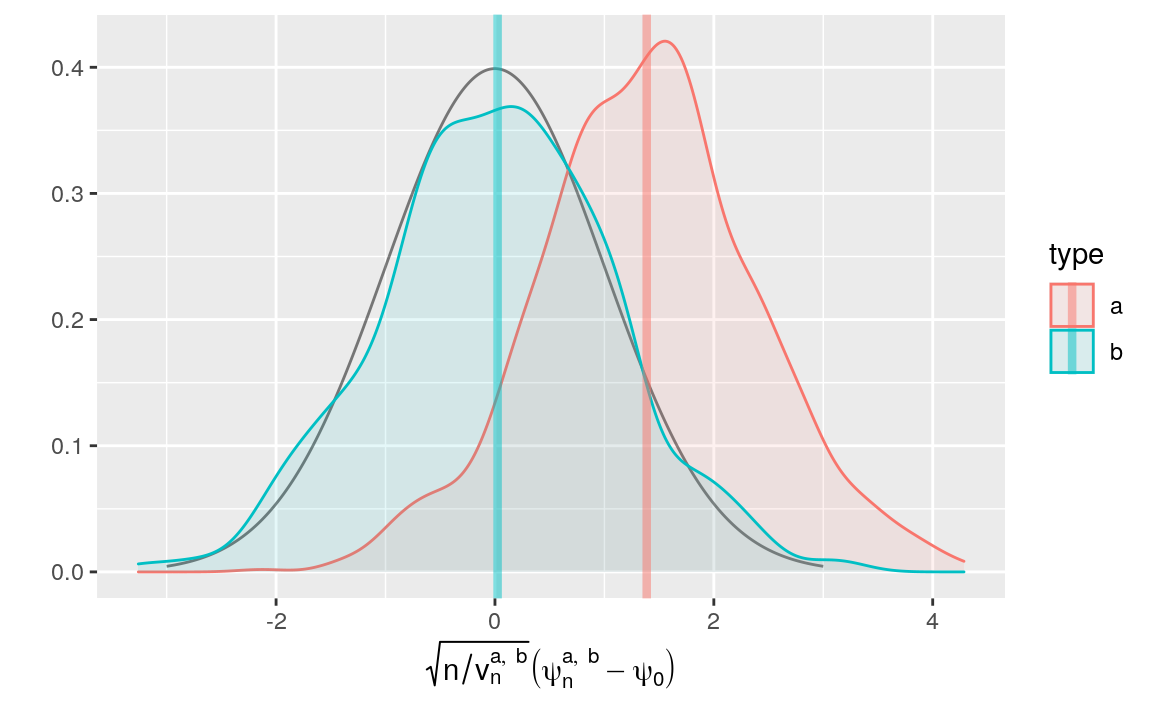
\includegraphics[width=0.7\linewidth]{img/known-Gbar-one-b-1} 

}

\caption{Kernel density estimators of the law of two estimators of \(\psi_{0}\) (recentered with respect to \(\psi_{0}\), and renormalized), one of them misconceived (a), the other assuming that \(\Gbar_{0}\) is known (b). Built based on 1000 independent realizations of each estimator.}\label{fig:known-Gbar-one-b}
\end{figure}

By the above chunk of code, the averages of \(\sqrt{n/v_{n}^{a}} (\psi_{n}^{a} - \psi_{0})\) and \(\sqrt{n/v_{n}^{b}} (\psi_{n}^{b} - \psi_{0})\)
computed across the realizations of the two estimators are respectively equal
to 1.387 and
0.024 (see \texttt{bias\_ab}). Interpreted as amounts of bias, those two
quantities are represented by vertical lines in Figure
\ref{fig:known-Gbar-one-b}. The red and blue bell-shaped curves represent the
empirical laws of \(\psi_{n}^{a}\) and \(\psi_{n}^{b}\) (recentered with respect
to \(\psi_{0}\), and renormalized) as estimated by kernel density estimation.
The latter is close to the black curve, which represents the standard normal
density.

\hypertarget{nuisance}{%
\chapter{Nuisance parameters}\label{nuisance}}

\hypertarget{anatomy}{%
\section{Anatomy of an expression}\label{anatomy}}

\index{nuisance~parameters|(}

From now, all the inference strategies that we will present unfold in two or
three stages. For all of them, the first stage consists in estimating a
selection of features of the law \(P_{0}\) of the experiment. Specifically, the
features are chosen among \(Q_{0,W}\) (the marginal law of \(W\) under \(P_{0}\)),
\(\Gbar_{0}\) (the conditional probability that \(A=1\) given \(W\) under \(P_{0}\))
and \(\Qbar_{0}\) (the conditional mean of \(Y\) given \(A\) and \(W\) under \(P_{0}\)).

In this context, because they are not the parameter of primary interest
(\emph{i.e.}, they are not the real-valued feature \(\Psi(P_{0})\)), they are often
referred to as \emph{nuisance parameters} of \(P_{0}\). The unflaterring expression
conveys the notion that their estimation is merely an intermediate step along
our path towards an inference of the target parameter.

As for the reason why \(Q_{0,W}\), \(\Gbar_{0}\) and \(\Qbar_{0}\) are singled out,
it is because of their role in the definition of \(\Psi\) and the efficient
influence curve \(D^{*}(P_{0})\).

\index{nuisance~parameters|)}

\hypertarget{an-algorithmic-stance}{%
\section{An algorithmic stance}\label{an-algorithmic-stance}}

\index{algorithm|(}

In general, we can view an estimator of any feature \(f_0\) of \(P_{0}\) as the
output of an algorithm \(\Algo\) that maps any element of

\begin{equation*}    \calM^{\text{empirical}}     \defq    \left\{\frac{1}{m}
\sum_{i=1}^{m} \Dirac(o_{i}) : m \geq 1, o_{1}, \ldots, o_{m} \in [0,1] \times
\{0,1\} \times [0,1]\right\} \end{equation*}

to the set \(\calF\) where \(f_{0}\) is known to live. Here,
\(\calM^{\text{empirical}}\) can be interpreted as the set of all possible
empirical measures summarizing the outcomes of any number of replications of
the experiment \(P_{0}\). In particular, \(P_{n}\) belongs to this set.

The \texttt{tlrider} package includes such template algorithms for the estimation of
\(Q_{0,W}\), \(\Gbar_{0}\) and \(\Qbar_{0}\). We illustrate how they work and their
use in the next sections.

\hypertarget{nuisance-QW}{%
\section{\texorpdfstring{\texttt{QW}}{QW}}\label{nuisance-QW}}

For instance, \texttt{estimate\_QW} is an algorithm \(\Algo_{Q_{W}}\) for the estimation
of the marginal law of \(W\) under \(P_{0}\) (to see its man page, simply run
\texttt{?estimate\_QW}). It is a map from \(\calM^{\text{empirical}}\) to the set of
laws on \([0,1]\). The following chunk of code estimates \(Q_{0,W}\) based on the
\(n = 1000\) first observations in \texttt{obs}:

\begin{Shaded}
\begin{Highlighting}[]
\NormalTok{QW\_hat }\OtherTok{\textless{}{-}} \FunctionTok{estimate\_QW}\NormalTok{(}\FunctionTok{head}\NormalTok{(obs, }\FloatTok{1e3}\NormalTok{))}
\end{Highlighting}
\end{Shaded}

It is easy to sample independent observations from \texttt{QW\_hat}. To do so, we
create an object of class \texttt{LAW} then set its marginal law of \(W\) to that
described by \texttt{QW\_hat} and specify its \texttt{sample\_from} feature:



\begin{Shaded}
\begin{Highlighting}[]
\NormalTok{empirical\_experiment }\OtherTok{\textless{}{-}} \FunctionTok{LAW}\NormalTok{()}
\FunctionTok{alter}\NormalTok{(empirical\_experiment, }\AttributeTok{QW =}\NormalTok{ QW\_hat)}
\FunctionTok{alter}\NormalTok{(empirical\_experiment, }\AttributeTok{sample\_from =} \ControlFlowTok{function}\NormalTok{(n) \{}
\NormalTok{  QW }\OtherTok{\textless{}{-}} \FunctionTok{get\_feature}\NormalTok{(empirical\_experiment, }\StringTok{"QW"}\NormalTok{)}
\NormalTok{  W }\OtherTok{\textless{}{-}} \FunctionTok{sample}\NormalTok{(}\FunctionTok{pull}\NormalTok{(QW, }\StringTok{"value"}\NormalTok{), n, }\AttributeTok{prob =} \FunctionTok{pull}\NormalTok{(QW, }\StringTok{"weight"}\NormalTok{))}
  \FunctionTok{cbind}\NormalTok{(}\AttributeTok{W =}\NormalTok{ W, }\AttributeTok{A =} \ConstantTok{NA}\NormalTok{, }\AttributeTok{Y =} \ConstantTok{NA}\NormalTok{)}
\NormalTok{\})}
\NormalTok{W }\OtherTok{\textless{}{-}} \FunctionTok{sample\_from}\NormalTok{(empirical\_experiment, }\FloatTok{1e3}\NormalTok{) }\SpecialCharTok{\%\textgreater{}\%}\NormalTok{ as\_tibble}

\NormalTok{W }\SpecialCharTok{\%\textgreater{}\%}
\FunctionTok{ggplot}\NormalTok{() }\SpecialCharTok{+}
  \FunctionTok{geom\_histogram}\NormalTok{(}\FunctionTok{aes}\NormalTok{(}\AttributeTok{x =}\NormalTok{ W, }\AttributeTok{y =} \FunctionTok{stat}\NormalTok{(density)), }\AttributeTok{bins =} \DecValTok{40}\NormalTok{) }\SpecialCharTok{+}
  \FunctionTok{stat\_function}\NormalTok{(}\AttributeTok{fun =} \FunctionTok{get\_feature}\NormalTok{(experiment, }\StringTok{"QW"}\NormalTok{), }\AttributeTok{col =} \StringTok{"red"}\NormalTok{)}
\end{Highlighting}
\end{Shaded}

\begin{figure}

{\centering 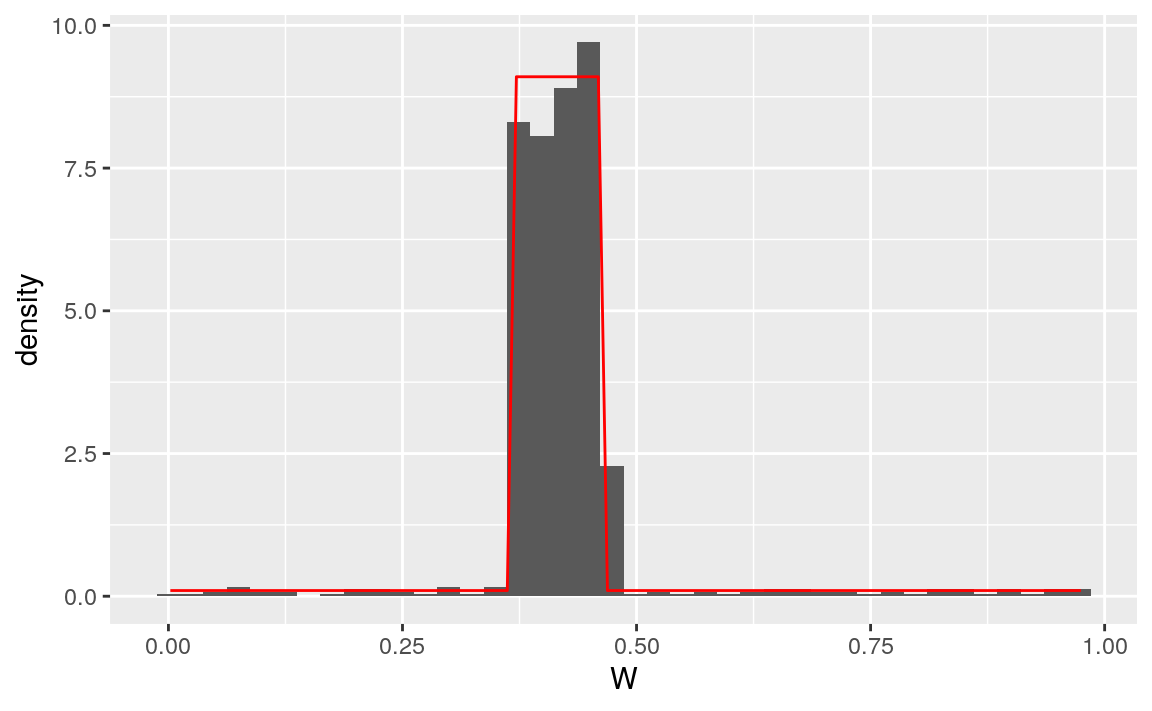
\includegraphics[width=0.7\linewidth]{img/estimate-QW-two-1} 

}

\caption{Histogram representing 1000 observations drawn independently from \texttt{QW\_hat}. The superimposed red curve is the true density of \(Q_{0,W}\).}\label{fig:estimate-QW-two}
\end{figure}

Note that all the \(W\)s sampled from \texttt{QW\_hat} fall in the set \(\{W_{1}, \ldots, W_{n}\}\) of observed \(W\)s in \texttt{obs} (an obvious fact given the definition of
the \texttt{sample\_from} feature of \texttt{empirical\_experiment}:

\begin{Shaded}
\begin{Highlighting}[]
\NormalTok{(}\FunctionTok{length}\NormalTok{(}\FunctionTok{intersect}\NormalTok{(}\FunctionTok{pull}\NormalTok{(W, W), }\FunctionTok{head}\NormalTok{(obs[, }\StringTok{"W"}\NormalTok{], }\FloatTok{1e3}\NormalTok{))))}
\CommentTok{\#\textgreater{} [1] 1000}
\end{Highlighting}
\end{Shaded}

This is because \texttt{estimate\_QW} estimates \(Q_{0,W}\) with its empirical
counterpart, \emph{i.e.},

\begin{equation*}\frac{1}{n} \sum_{i=1}^{n} \Dirac(W_{i}).\end{equation*}

\hypertarget{nuisance-Gbar}{%
\section{\texorpdfstring{\texttt{Gbar}}{Gbar}}\label{nuisance-Gbar}}

Another template algorithm is built-in into \texttt{tlrider}: \texttt{estimate\_Gbar} (to see
its man page, simply run \texttt{?estimate\_Gbar}). Unlike \texttt{estimate\_QW},
\texttt{estimate\_Gbar} needs further specification of the algorithm. The package also
includes examples of such specifications.

There are two sorts of specifications, of which we say that they are either
\emph{working model-based} or \emph{machine learning-based}. We discuss the former sort
in the next subsection. The latter sort is discussed in Section
\ref{nuisance-Qbar}.

\hypertarget{logis-loss}{%
\subsection{Working model-based algorithms}\label{logis-loss}}

\index{algorithm!working~model|(}

Let us take a look at \texttt{working\_model\_G\_one} for instance:

\begin{Shaded}
\begin{Highlighting}[]
\NormalTok{working\_model\_G\_one}
\CommentTok{\#\textgreater{} $model}
\CommentTok{\#\textgreater{} function (...) }
\CommentTok{\#\textgreater{} \{}
\CommentTok{\#\textgreater{}     trim\_glm\_fit(glm(family = binomial(), ...))}
\CommentTok{\#\textgreater{} \}}
\CommentTok{\#\textgreater{} \textless{}environment: 0x55d8a00b8520\textgreater{}}
\CommentTok{\#\textgreater{} }
\CommentTok{\#\textgreater{} $formula}
\CommentTok{\#\textgreater{} A \textasciitilde{} I(W\^{}0.5) + I(abs(W {-} 5/12)\^{}0.5) + I(W\^{}1) + I(abs(W {-} 5/12)\^{}1) + }
\CommentTok{\#\textgreater{}     I(W\^{}1.5) + I(abs(W {-} 5/12)\^{}1.5)}
\CommentTok{\#\textgreater{} \textless{}environment: 0x55d8a00b8520\textgreater{}}
\CommentTok{\#\textgreater{} }
\CommentTok{\#\textgreater{} $type\_of\_preds}
\CommentTok{\#\textgreater{} [1] "response"}
\CommentTok{\#\textgreater{} }
\CommentTok{\#\textgreater{} attr(,"ML")}
\CommentTok{\#\textgreater{} [1] FALSE}
\end{Highlighting}
\end{Shaded}

and focus on its \texttt{model} and \texttt{formula} attributes. The former relies on the
\texttt{glm} and \texttt{binomial} functions from \texttt{base} \texttt{R}, and on \texttt{trim\_glm\_fit} (which
removes information that we do not need from the standard output of \texttt{glm},
simply run \texttt{?trim\_glm\_fit} to see the function's man page). The latter is a
\texttt{formula} that characterizes what we call a \emph{working model} for \(\Gbar_{0}\).

In words, by using \texttt{working\_model\_G\_one} we implicitly choose the so-called
logistic (or negative binomial) loss function \(L_{a}\) given by

\begin{equation} 
\label{eq:logis-loss} -L_{a}(f)(A,W) \defq A \log f(W) + (1 - A)
\log (1 - f(W)) 
\end{equation}

for any function \(f : [0,1] \to [0,1]\) paired with the working model
\begin{equation*}   \calF_{1}   \defq    \left\{f_{\theta}   :   \theta   \in
\bbR^{7}\right\}  \end{equation*} where, for any \(\theta \in \bbR^{7}\),
\begin{equation*}\logit  f_{\theta}  (W)  \defq \theta_{0}  +  \sum_{j=1}^{3}
\left(\theta_{j} W^{j/2} + \theta_{3+j} |W - 5/12|^{j/2}\right).\end{equation*}

We acted as oracles when we specified the working model: it is
\emph{well-specified}, \emph{i.e.}, it happens that \(\Gbar_{0}\) is the unique minimizer
of the risk entailed by \(L_{a}\) over \(\calF_{1}\): \begin{equation*}\Gbar_{0} =
\mathop{\arg\min}_{f_{\theta}        \in        \calF_{1}}        \Exp_{P_{0}}
\left(L_{a}(f_{\theta})(A,W)\right).\end{equation*} Therefore, the estimator
\(\Gbar_{n}\) obtained by minimizing the empirical risk\index{well/mis-specified}

\begin{equation*}
\Exp_{P_{n}} \left(L_{a}(f_{\theta})(A,W)\right)  = \frac{1}{n} \sum_{i=1}^{n}
L_{a}(f_{\theta})(A_{i},W_{i})
\end{equation*}

over \(\calF_{1}\) estimates \(\Gbar_{0}\) consistently.

Of course, it is seldom certain in real life that the target feature, here
\(\Gbar_{0}\), belongs to the working model.\footnote{In fact, if one knows nothing
  about the feature, then it is \emph{certain} that it does not belong to whichever
  small finite-dimensional working model we may come up with.} Suppose for
instance that we choose a small finite-dimensional working model \(\calF_{2}\)
without acting as an oracle. Then consistency certainly fails to hold.
However, if \(\Gbar_{0}\) can nevertheless be \emph{projected} unambiguously onto
\(\calF_{2}\) (an assumption that cannot be checked), then the estimator might
converge to the projection.

\hypertarget{algo-Gbar-one}{%
\subsection{Visualization}\label{algo-Gbar-one}}

To illustrate the use of the algorithm \(\Algo_{\Gbar,1}\) obtained by combining
\texttt{estimate\_Gbar} and \texttt{working\_model\_G\_one}, let us estimate \(\Gbar_{0}\) based
on the first \(n = 1000\) observations in \texttt{obs}:

\begin{Shaded}
\begin{Highlighting}[]
\NormalTok{Gbar\_hat }\OtherTok{\textless{}{-}} \FunctionTok{estimate\_Gbar}\NormalTok{(}\FunctionTok{head}\NormalTok{(obs, }\FloatTok{1e3}\NormalTok{), }\AttributeTok{algorithm =}\NormalTok{ working\_model\_G\_one)}
\end{Highlighting}
\end{Shaded}

Using \texttt{compute\_Gbar\_hat\_W}\footnote{See also the companion function
  \texttt{compute\_lGbar\_hat\_AW} (run \texttt{?compute\_lGbar\_hat\_AW} to see its man page.}
(simply run \texttt{?compute\_Gbar\_hat\_W} to see its man page) makes it is easy to
compare visually the estimator \(\Gbar_{n} \defq \Algo_{\Gbar,1}(P_{n})\) with
its target \(\Gbar_0\):



\begin{Shaded}
\begin{Highlighting}[]
\FunctionTok{tibble}\NormalTok{(}\AttributeTok{w =} \FunctionTok{seq}\NormalTok{(}\DecValTok{0}\NormalTok{, }\DecValTok{1}\NormalTok{, }\AttributeTok{length.out =} \FloatTok{1e3}\NormalTok{)) }\SpecialCharTok{\%\textgreater{}\%}
  \FunctionTok{mutate}\NormalTok{(}\StringTok{"truth"} \OtherTok{=} \FunctionTok{Gbar}\NormalTok{(w),}
         \StringTok{"estimated"} \OtherTok{=} \FunctionTok{compute\_Gbar\_hatW}\NormalTok{(w, Gbar\_hat)) }\SpecialCharTok{\%\textgreater{}\%}
  \FunctionTok{pivot\_longer}\NormalTok{(}\SpecialCharTok{{-}}\NormalTok{w, }\AttributeTok{names\_to =} \StringTok{"f"}\NormalTok{, }\AttributeTok{values\_to =} \StringTok{"value"}\NormalTok{) }\SpecialCharTok{\%\textgreater{}\%}
  \FunctionTok{ggplot}\NormalTok{() }\SpecialCharTok{+}
  \FunctionTok{geom\_line}\NormalTok{(}\FunctionTok{aes}\NormalTok{(}\AttributeTok{x =}\NormalTok{ w, }\AttributeTok{y =}\NormalTok{ value, }\AttributeTok{color =}\NormalTok{ f), }\AttributeTok{size =} \DecValTok{1}\NormalTok{) }\SpecialCharTok{+}
  \FunctionTok{labs}\NormalTok{(}\AttributeTok{y =} \StringTok{"f(w)"}\NormalTok{,}
       \AttributeTok{title =} \FunctionTok{bquote}\NormalTok{(}\StringTok{"Visualizing"} \SpecialCharTok{\textasciitilde{}} \FunctionTok{bar}\NormalTok{(G)[}\DecValTok{0}\NormalTok{] }\SpecialCharTok{\textasciitilde{}} \StringTok{"and"} \SpecialCharTok{\textasciitilde{}} \FunctionTok{hat}\NormalTok{(G)[n])) }\SpecialCharTok{+}
  \FunctionTok{ylim}\NormalTok{(}\ConstantTok{NA}\NormalTok{, }\DecValTok{1}\NormalTok{)}
\end{Highlighting}
\end{Shaded}

\begin{figure}

{\centering 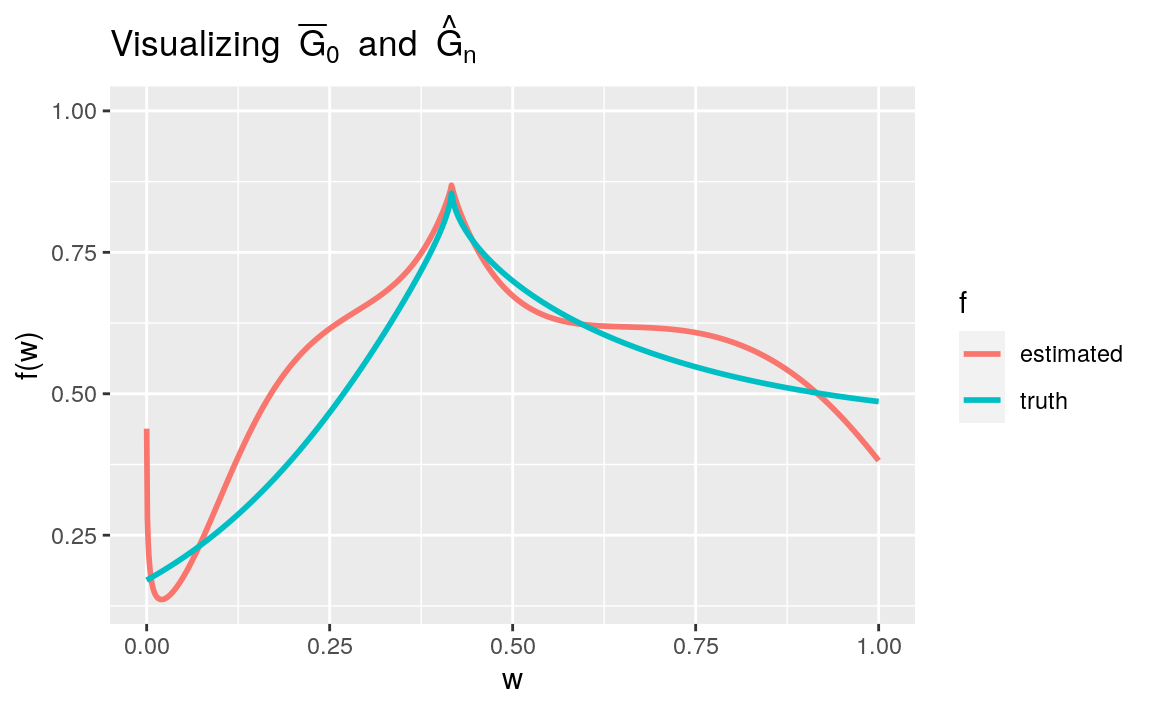
\includegraphics[width=0.7\linewidth]{img/estimate-Gbar-three-1} 

}

\caption{Comparing \(\Gbar_{n}\defq \Algo_{\Gbar,1}(P_{n})\) and \(\Gbar_{0}\). The estimator is consistent because the algorithm relies on a working model that is correctly specified.}\label{fig:estimate-Gbar-three}
\end{figure}

\hypertarget{nuisance-Qbar-wm}{%
\section{\texorpdfstring{⚙ \gear \texttt{Qbar}, working model-based algorithms}{⚙ Qbar, working model-based algorithms}}\label{nuisance-Qbar-wm}}

A third template algorithm is built-in into \texttt{tlrider}: \texttt{estimate\_Qbar} (to see
its man page, simply run \texttt{?estimate\_Qbar}). Like \texttt{estimate\_Gbar},
\texttt{estimate\_Qbar} needs further specification of the algorithm. The package also
includes examples of such specifications, which can also be either working
model-based (see Section \ref{nuisance-Gbar}) or machine learning-based (see
Sections \ref{nuisance-Qbar} and \ref{nuisance-Qbar-ml-exo}).

There are built-in specifications similar to \texttt{working\_model\_G\_one}, \emph{e.g.},

\begin{Shaded}
\begin{Highlighting}[]
\NormalTok{working\_model\_Q\_one}
\CommentTok{\#\textgreater{} $model}
\CommentTok{\#\textgreater{} function (...) }
\CommentTok{\#\textgreater{} \{}
\CommentTok{\#\textgreater{}     trim\_glm\_fit(glm(family = binomial(), ...))}
\CommentTok{\#\textgreater{} \}}
\CommentTok{\#\textgreater{} \textless{}environment: 0x55d8a00b8520\textgreater{}}
\CommentTok{\#\textgreater{} }
\CommentTok{\#\textgreater{} $formula}
\CommentTok{\#\textgreater{} Y \textasciitilde{} A * (I(W\^{}0.5) + I(W\^{}1) + I(W\^{}1.5))}
\CommentTok{\#\textgreater{} \textless{}environment: 0x55d8a00b8520\textgreater{}}
\CommentTok{\#\textgreater{} }
\CommentTok{\#\textgreater{} $type\_of\_preds}
\CommentTok{\#\textgreater{} [1] "response"}
\CommentTok{\#\textgreater{} }
\CommentTok{\#\textgreater{} attr(,"ML")}
\CommentTok{\#\textgreater{} [1] FALSE}
\CommentTok{\#\textgreater{} attr(,"stratify")}
\CommentTok{\#\textgreater{} [1] FALSE}
\end{Highlighting}
\end{Shaded}

\begin{enumerate}
\def\labelenumi{\arabic{enumi}.}
\tightlist
\item
  Drawing inspiration from Section \ref{nuisance-Gbar}, comment upon and use
  the algorithm \(\Algo_{\Qbar,1}\) obtained by combining \texttt{estimate\_Gbar} and
  \texttt{working\_model\_Q\_one}.
\end{enumerate}

\index{algorithm!working~model|)}

\hypertarget{nuisance-Qbar}{%
\section{\texorpdfstring{\texttt{Qbar}}{Qbar}}\label{nuisance-Qbar}}

\hypertarget{qbar-machine-learning-based-algorithms}{%
\subsection{\texorpdfstring{\texttt{Qbar}, machine learning-based algorithms}{Qbar, machine learning-based algorithms}}\label{qbar-machine-learning-based-algorithms}}

\index{algorithm!machine~learning|(}

We explained how algorithm \(\Algo_{\Gbar,1}\) is based on a working model (and
\emph{you} did for \(\Algo_{\Qbar,1}\)). It is not the case that all algorithms are
based on working models in the same (admittedly rather narrow) sense. We
propose to say that those algorithms that are not based on working models like
\(\Algo_{\Gbar,1}\), for instance, are instead \emph{machine learning-based}.

Typically, machine learning-based algorithms are more data-adaptive; they rely
on larger working models, and/or fine-tune parameters that must be calibrated,
\emph{e.g.} by cross-validation.\index{algorithm!cross-validation} Furthermore,
they call for being stacked\index{algorithm!machine~learning!stacking},
\emph{i.e.}, combined by means of another outer algorithm (involving
cross-validation) into a more powerful machine learning-based
\emph{meta-algorithm}. The super
learning\index{algorithm!machine~learning!super~learning} methodology is a
popular stacking algorithm.

We will elaborate further on this important topic in another forthcoming part
and merely touch upon it in Section \ref{meta-learning}. Here, we simply
illustrate the concept with two specifications built-in into \texttt{tlrider}. Based
on the \emph{\(k\)-nearest neighbors} non-parametric estimating methodology, the
first one is discussed in the next subsection. Based on \emph{boosted trees},
another non-parametric estimating methodology, the second one is used in the
exercise that follows the next subsection.

\hypertarget{Qbar-knn-algo}{%
\subsection{\texorpdfstring{\texttt{Qbar}, kNN algorithm}{Qbar, kNN algorithm}}\label{Qbar-knn-algo}}

Algorithm \(\Algo_{\Qbar,\text{kNN}}\) is obtained by combining \texttt{estimate\_Qbar}
and \texttt{kknn\_algo}. The training of \(\Algo_{\Qbar,\text{kNN}}\) (\emph{i.e.}, the
making of the output \(\Algo_{\Qbar,\text{kNN}} (P_{n})\) is implemented based
on function \texttt{caret::train} of the \texttt{caret} (classification and regression
training) package (to see its man page, simply run \texttt{?caret::train}). Some
additional specifications are provided in \texttt{kknn\_grid} and \texttt{kknn\_control}.

In a nutshell, \(\Algo_{\Qbar,\text{kNN}}\) estimates \(\Qbar_{0}(1,\cdot)\) and
\(\Qbar_{0}(0,\cdot)\) separately. Each of them is estimated by applying the
\(k\)-nearest neighbors methodology as it is implemented in function
\texttt{kknn::train.kknn} from the \texttt{kknn} package (to see its man page, simply run
\texttt{?kknn::train.kknn}).\footnote{Specifically, argument \texttt{kmax} (maximum number of
  neighbors considered) is set to 5, argument \texttt{distance} (parameter of the
  Minkowski distance) is set to 2, and argument \texttt{kernel} is set to \texttt{gaussian}.
  The best value of \(k\) is chosen between 1 and \texttt{kmax} by leave-one-out. No
  outer cross-validation is needed.} The following chunk of code trains
algorithm \(\Algo_{\Qbar,\text{kNN}}\) on \(P_{n}\):

\begin{Shaded}
\begin{Highlighting}[]
\NormalTok{Qbar\_hat\_kknn }\OtherTok{\textless{}{-}} \FunctionTok{estimate\_Qbar}\NormalTok{(}\FunctionTok{head}\NormalTok{(obs, }\FloatTok{1e3}\NormalTok{),}
                               \AttributeTok{algorithm =}\NormalTok{ kknn\_algo,}
                               \AttributeTok{trControl =}\NormalTok{ kknn\_control,}
                               \AttributeTok{tuneGrid =}\NormalTok{ kknn\_grid)}
\end{Highlighting}
\end{Shaded}

Using \texttt{compute\_Qbar\_hat\_AW} (simply run \texttt{?compute\_Qbar\_hat\_AW} to see its man
page) makes it is easy to compare visually the estimator \(\Qbar_{n,\text{kNN}} \defq \Algo_{\Qbar,\text{kNN}}(P_{n})\) with its target \(\Qbar0\), see Figure
\ref{fig:estimate-Qbar-five}.

\begin{Shaded}
\begin{Highlighting}[]
\NormalTok{fig }\OtherTok{\textless{}{-}} \FunctionTok{tibble}\NormalTok{(}\AttributeTok{w =} \FunctionTok{seq}\NormalTok{(}\DecValTok{0}\NormalTok{, }\DecValTok{1}\NormalTok{, }\AttributeTok{length.out =} \FloatTok{1e3}\NormalTok{),}
              \AttributeTok{truth\_1 =} \FunctionTok{Qbar}\NormalTok{(}\FunctionTok{cbind}\NormalTok{(}\AttributeTok{A =} \DecValTok{1}\NormalTok{, }\AttributeTok{W =}\NormalTok{ w)),}
              \AttributeTok{truth\_0 =} \FunctionTok{Qbar}\NormalTok{(}\FunctionTok{cbind}\NormalTok{(}\AttributeTok{A =} \DecValTok{0}\NormalTok{, }\AttributeTok{W =}\NormalTok{ w)),}
              \AttributeTok{kNN\_1 =} \FunctionTok{compute\_Qbar\_hatAW}\NormalTok{(}\DecValTok{1}\NormalTok{, w, Qbar\_hat\_kknn),}
              \AttributeTok{kNN\_0 =} \FunctionTok{compute\_Qbar\_hatAW}\NormalTok{(}\DecValTok{0}\NormalTok{, w, Qbar\_hat\_kknn))}
\end{Highlighting}
\end{Shaded}

\hypertarget{boosted-trees}{%
\subsection{\texorpdfstring{\texttt{Qbar}, boosted trees algorithm}{Qbar, boosted trees algorithm}}\label{boosted-trees}}

Algorithm \(\Algo_{\Qbar,\text{trees}}\) is obtained by combining
\texttt{estimate\_Qbar} and \texttt{bstTree\_algo}. The training of
\(\Algo_{\Qbar,\text{trees}}\) (\emph{i.e.}, the making of the output
\(\Algo_{\Qbar,\text{trees}} (P_{n})\) is implemented based on function
\texttt{caret::train} of the \texttt{caret} package. Some additional specifications are
provided in \texttt{bstTree\_grid} and \texttt{bstTree\_control}.

In a nutshell, \(\Algo_{\Qbar,\text{trees}}\) estimates \(\Qbar_{0}(1,\cdot)\) and
\(\Qbar_{0}(0,\cdot)\) separately. Each of them is estimated by boosted trees
as implemented in function \texttt{bst::bst} from the \texttt{bst} (gradient boosting)
package (to see its man page, simply run \texttt{?bst::bst}).\footnote{Specifically, argument
  \texttt{mstop} (number of boosting iterations for prediction) is one among 10, 20 and
  30; argument \texttt{nu} (stepsize of the shrinkage parameter) is one among 0.1 and
  0.2; argument \texttt{maxdepth} (maximum depth of the base learner, a tree) is one
  among 1, 2 and 5. An outer 10-fold cross-validation is carried out to select
  the best combination of fine-tune parameters.} The following chunk of code
trains algorithm \(\Algo_{\Qbar,\text{trees}}\) on \(P_{n}\), and reveals what are
the optimal fine-tune parameters for the estimation of \(\Qbar_{0}(1,\cdot)\)
and \(\Qbar_{0}(0,\cdot)\):

\begin{Shaded}
\begin{Highlighting}[]
\NormalTok{Qbar\_hat\_trees }\OtherTok{\textless{}{-}} \FunctionTok{estimate\_Qbar}\NormalTok{(}\FunctionTok{head}\NormalTok{(obs, }\FloatTok{1e3}\NormalTok{),}
                                \AttributeTok{algorithm =}\NormalTok{ bstTree\_algo,}
                                \AttributeTok{trControl =}\NormalTok{ bstTree\_control,}
                                \AttributeTok{tuneGrid =}\NormalTok{ bstTree\_grid)}

\NormalTok{Qbar\_hat\_trees }\SpecialCharTok{\%\textgreater{}\%} \FunctionTok{filter}\NormalTok{(a }\SpecialCharTok{==} \StringTok{"one"}\NormalTok{) }\SpecialCharTok{\%\textgreater{}\%} \FunctionTok{pull}\NormalTok{(fit) }\SpecialCharTok{\%\textgreater{}\%}
\NormalTok{  capture.output }\SpecialCharTok{\%\textgreater{}\%} \FunctionTok{tail}\NormalTok{(}\DecValTok{3}\NormalTok{) }\SpecialCharTok{\%\textgreater{}\%} \FunctionTok{str\_wrap}\NormalTok{(}\AttributeTok{width =} \DecValTok{60}\NormalTok{) }\SpecialCharTok{\%\textgreater{}\%}\NormalTok{ cat}
\CommentTok{\#\textgreater{} RMSE was used to select the optimal model using the smallest}
\CommentTok{\#\textgreater{} value. The final values used for the model were mstop = 30,}
\CommentTok{\#\textgreater{} maxdepth = 2 and nu = 0.2.}
                                                             
\NormalTok{Qbar\_hat\_trees }\SpecialCharTok{\%\textgreater{}\%} \FunctionTok{filter}\NormalTok{(a }\SpecialCharTok{==} \StringTok{"zero"}\NormalTok{) }\SpecialCharTok{\%\textgreater{}\%} \FunctionTok{pull}\NormalTok{(fit) }\SpecialCharTok{\%\textgreater{}\%}
\NormalTok{  capture.output }\SpecialCharTok{\%\textgreater{}\%} \FunctionTok{tail}\NormalTok{(}\DecValTok{3}\NormalTok{) }\SpecialCharTok{\%\textgreater{}\%} \FunctionTok{str\_wrap}\NormalTok{(}\AttributeTok{width =} \DecValTok{60}\NormalTok{) }\SpecialCharTok{\%\textgreater{}\%}\NormalTok{ cat}
\CommentTok{\#\textgreater{} RMSE was used to select the optimal model using the smallest}
\CommentTok{\#\textgreater{} value. The final values used for the model were mstop = 30,}
\CommentTok{\#\textgreater{} maxdepth = 1 and nu = 0.1.}
\end{Highlighting}
\end{Shaded}

We can compare visually the estimators \(\Qbar_{n,\text{kNN}}\),
\(\Qbar_{n,\text{trees}} \defq \Algo_{\Qbar,\text{trees}}(P_{n})\) with its
target \(\Qbar_0\), see Figure \ref{fig:estimate-Qbar-five}. In summary,
\(\Qbar_{n,\text{kNN}}\) is rather good, though very variable at the vincinity
of the break points. As for \(\Qbar_{n,\text{trees}}\), it does not seem to
capture the shape of its target.



\begin{Shaded}
\begin{Highlighting}[]
\NormalTok{fig }\SpecialCharTok{\%\textgreater{}\%}
  \FunctionTok{mutate}\NormalTok{(}\AttributeTok{trees\_1 =} \FunctionTok{compute\_Qbar\_hatAW}\NormalTok{(}\DecValTok{1}\NormalTok{, w, Qbar\_hat\_trees),}
         \AttributeTok{trees\_0 =} \FunctionTok{compute\_Qbar\_hatAW}\NormalTok{(}\DecValTok{0}\NormalTok{, w, Qbar\_hat\_trees)) }\SpecialCharTok{\%\textgreater{}\%}
  \FunctionTok{pivot\_longer}\NormalTok{(}\SpecialCharTok{{-}}\NormalTok{w, }\AttributeTok{names\_to =} \StringTok{"f"}\NormalTok{, }\AttributeTok{values\_to =} \StringTok{"value"}\NormalTok{) }\SpecialCharTok{\%\textgreater{}\%}
  \FunctionTok{extract}\NormalTok{(f, }\FunctionTok{c}\NormalTok{(}\StringTok{"f"}\NormalTok{, }\StringTok{"a"}\NormalTok{), }\StringTok{"([\^{}\_]+)\_([01]+)"}\NormalTok{) }\SpecialCharTok{\%\textgreater{}\%}
  \FunctionTok{mutate}\NormalTok{(}\AttributeTok{a =} \FunctionTok{paste0}\NormalTok{(}\StringTok{"a="}\NormalTok{, a)) }\SpecialCharTok{\%\textgreater{}\%}
\NormalTok{  ggplot }\SpecialCharTok{+}
  \FunctionTok{geom\_line}\NormalTok{(}\FunctionTok{aes}\NormalTok{(}\AttributeTok{x =}\NormalTok{ w, }\AttributeTok{y =}\NormalTok{ value, }\AttributeTok{color =}\NormalTok{ f), }\AttributeTok{size =} \DecValTok{1}\NormalTok{) }\SpecialCharTok{+}
  \FunctionTok{labs}\NormalTok{(}\AttributeTok{y =} \StringTok{"f(w)"}\NormalTok{,}
       \AttributeTok{title =} \FunctionTok{bquote}\NormalTok{(}\StringTok{"Visualizing"} \SpecialCharTok{\textasciitilde{}} \FunctionTok{bar}\NormalTok{(Q)[}\DecValTok{0}\NormalTok{] }\SpecialCharTok{\textasciitilde{}} \StringTok{"and its estimators"}\NormalTok{)) }\SpecialCharTok{+}
  \FunctionTok{ylim}\NormalTok{(}\ConstantTok{NA}\NormalTok{, }\DecValTok{1}\NormalTok{) }\SpecialCharTok{+}
  \FunctionTok{facet\_wrap}\NormalTok{(}\SpecialCharTok{\textasciitilde{}}\NormalTok{ a)}
\end{Highlighting}
\end{Shaded}

\begin{figure}

{\centering 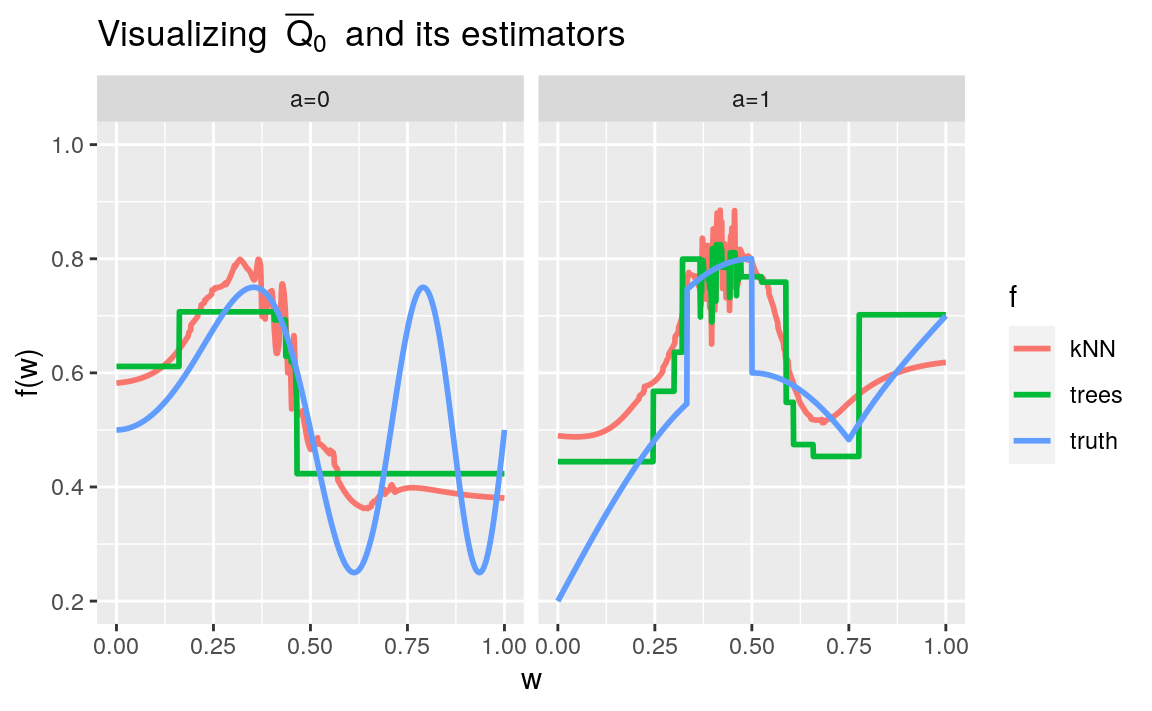
\includegraphics[width=0.7\linewidth]{img/estimate-Qbar-five-1} 

}

\caption{Comparing to their target two (machine learning-based) estimators of \(\Qbar_{0}\), one based on the \(k\)-nearest neighbors and the other on boosted trees.}\label{fig:estimate-Qbar-five}
\end{figure}

\hypertarget{nuisance-Qbar-ml-exo}{%
\section{\texorpdfstring{⚙ \gear ☡ \stixdanger{} \texttt{Qbar}, machine learning-based algorithms}{⚙ ☡  Qbar, machine learning-based algorithms}}\label{nuisance-Qbar-ml-exo}}

\begin{enumerate}
\def\labelenumi{\arabic{enumi}.}
\item
  Using \texttt{estimate\_Q}, make your own machine learning-based algorithm for the
  estimation of \(\Qbar_{0}\).
\item
  Train your algorithm on the same data set as \(\Algo_{\Qbar,\text{kNN}}\) and
  \(\Algo_{\Qbar,\text{trees}}\). If, like \(\Algo_{\Qbar,\text{trees}}\), your
  algorithm includes a fine-tuning procedure, comment upon the optimal,
  data-driven specification.
\item
  Plot your estimators of \(\Qbar_{0}(1,\cdot)\) and \(\Qbar_{0}(0,\cdot)\) on
  Figure \ref{fig:estimate-Qbar-five}.
\end{enumerate}

\hypertarget{meta-learning}{%
\section{Meta-learning/super learning}\label{meta-learning}}

Without a great deal of previous experience or scientific expertise, it would
have likely been difficult for us to \emph{a priori} postulate which of the two
above machine learning algorithms (or indeed the algorithm based on a working
model) would perform better for estimation of \(\bar{Q}_0\). Rather than
committing to one single algorithm, we may instead wish to resort to
meta-learning or super learning. In this approach, one specifies a \emph{library}
of candidate algorithms for estimating a given nuisance parameter.
Cross-validation is used to determine an \emph{ensemble} (\emph{e.g.} convex
combination) of the algorithms that yields the best fit to the underlying
function. In this way, one can learn in real time which algorithms tend to
fit the data best and shift attention towards those algorithms.

\index{algorithm!machine~learning|)}

\index{algorithm|)}

\hypertarget{naive-estimators}{%
\chapter{Two ``naive'' inference strategies}\label{naive-estimators}}

\hypertarget{why-naive}{%
\section{Why ``naive''?}\label{why-naive}}

In this section, we present and discuss two strategies for the inference of
\(\Psi(P_{0})\). In light of Section \ref{anatomy}, both unfold in \emph{two}
stages. During the first stage, some features among \(Q_{0,W}\), \(\Gbar_{0}\)
and \(\Qbar_{0}\) (the \(\Psi\)-specific nuisance parameters, see Section
\ref{nuisance})\index{nuisance~parameters} are estimated. During the second
stage, these estimators are used to build estimators of \(\Psi(P_{0})\).

Although the strategies sound well conceived, a theoretical analysis reveals
that they lack a third stage trying to correct an inherent flaw. They are thus
said \emph{naive}. The analysis and a first \emph{modus operandi} are presented in
Section \ref{analysis-of-plug-in}.

\hypertarget{known-gbar-second-pass}{%
\section{IPTW estimator}\label{known-gbar-second-pass}}

\hypertarget{unknown-gbar-constr}{%
\subsection{Construction and computation}\label{unknown-gbar-constr}}

In Section \ref{known-gbar-first-pass}, we developed an IPTW estimator,
\(\psi_{n}^{b}\), \emph{assuming that} we knew \(\Gbar_{0}\) beforehand. What if we
did not? Obviously, we could estimate it and substitute the estimator of
\(\ell\Gbar_{0}\) for \(\ell\Gbar_{0}\) in \eqref{eq:psi-n-b}.

Let \(\Algo_{\Gbar}\) be an algorithm designed for the estimation of \(\Gbar_{0}\)
(see Section \ref{nuisance-Gbar}). We denote by \(\Gbar_{n} \defq \Algo_{\Gbar}(P_{n})\) the output of the algorithm trained on \(P_{n}\), and by
\(\ell\Gbar_{n}\) the resulting (empirical) function given by

\begin{equation*}
\ell\Gbar_{n}(A,W) \defq A \Gbar_{n}(W) + (1-A) (1 - \Gbar_{n}(W)).
\end{equation*}

In light of \eqref{eq:psi-n-b}, we introduce

\begin{equation*}
\psi_{n}^{c}   \defq   \frac{1}{n}    \sum_{i=1}^{n}   \left(\frac{2A_{i}   -
1}{\ell\Gbar_{n}(A_{i}, W_{i})} Y_{i}\right).
\end{equation*}

From a computational point of view, the \texttt{tlrider} package makes it easy to
build \(\psi_{n}^{c}\). Recall that

\begin{Shaded}
\begin{Highlighting}[]
\FunctionTok{compute\_iptw}\NormalTok{(}\FunctionTok{head}\NormalTok{(obs, }\FloatTok{1e3}\NormalTok{), Gbar)}
\end{Highlighting}
\end{Shaded}

implements the computation of \(\psi_{n}^{b}\) based on the \(n=1000\) first
observations stored in \texttt{obs}, using the true feature \(\Gbar_{0}\) stored in
\texttt{Gbar}, see Section \ref{empirical-inves-IPTW} and the construction of
\texttt{psi\_hat\_ab}. Similarly,

\begin{Shaded}
\begin{Highlighting}[]
\NormalTok{Gbar\_hat }\OtherTok{\textless{}{-}} \FunctionTok{estimate\_Gbar}\NormalTok{(}\FunctionTok{head}\NormalTok{(obs, }\FloatTok{1e3}\NormalTok{), working\_model\_G\_one)}
\FunctionTok{compute\_iptw}\NormalTok{(}\FunctionTok{head}\NormalTok{(obs, }\FloatTok{1e3}\NormalTok{), }\FunctionTok{wrapper}\NormalTok{(Gbar\_hat)) }\SpecialCharTok{\%\textgreater{}\%} \FunctionTok{pull}\NormalTok{(psi\_n)}
\CommentTok{\#\textgreater{} [1] 0.104}
\end{Highlighting}
\end{Shaded}

implements \emph{(i)} the estimation of \(\Gbar_{0}\) with \(\Gbar_{n}\)/\texttt{Gbar\_hat}
using algorithm \(\Algo_{\Gbar,1}\) (first line) then \emph{(ii)} the computation of
\(\psi_{n}^{c}\) (second line), both based on the same observations as above.

Note how we use function \texttt{wrapper} (simply run \texttt{?wrapper} to see its man
page).

\hypertarget{elementary-stat-prop-iptw}{%
\subsection{Elementary statistical properties}\label{elementary-stat-prop-iptw}}

Because \(\Gbar_{n}\) minimizes the empirical risk over a finite-dimensional,
identifiable, and \textbf{well-specified} working model, \(\sqrt{n} (\psi_{n}^{c} - \psi_{0})\) converges in law to a centered Gaussian law.\index{identifiability}
Moreover, the asymptotic variance of \(\sqrt{n} (\psi_{n}^{c} - \psi_{0})\) is
\textbf{conservatively}\footnote{In words, \(v_{n}^{c}\) converges to an upper-bound of the
  true asymptotic variance.}\index{conservative} estimated
with\index{well/mis-specified}

\begin{align*}            v_{n}^{c}            &\defq            \Var_{P_{n}}
\left(\frac{2A-1}{\ell\Gbar_{n}(A,W)}Y\right)      \\      &=      \frac{1}{n}
\sum_{i=1}^{n}\left(\frac{2A_{i}-1}{\ell\Gbar_{n}   (A_{i},W_{i})}   Y_{i}   -
\psi_{n}^{c}\right)^{2}.  \end{align*}

We investigate \emph{empirically} the statistical behavior of \(\psi_{n}^{c}\) in
Section \ref{empirical-inves-IPTW-bis}. For an analysis of the reason why
\(v_{n}^{c}\) is a conservative estimator of the asymptotic variance of
\(\sqrt{n} (\psi_{n}^{c} - \psi_{0})\), see \protect\hyperlink{iptw-est-var}{there} in Appendix
\ref{iptw-est-var}.

Before proceeding, let us touch upon what would have happened if we had used a
less amenable algorithm \(\Algo_{\Gbar}\). For instance, \(\Algo_{\Gbar}\) could
still be well-specified\footnote{Well-specified \emph{e.g.} in the sense that the target
  \(\Gbar_{0}\) of \(\Algo_{\Gbar}\) belongs to the closure of the algorithm's image
  \(\Algo_{\Gbar}(\calM^{\text{empirical}})\) or, in other words, can be
  approximated arbitrarily well by an output of the algorithm.} but so
\emph{versatile/complex} (as opposed to being based on well-behaved,
finite-dimensional parametric model) that the estimator \(\Gbar_{n}\), though
still consistent, would converge slowly to its target. Then, root-\(n\)
consistency would fail to hold. Or \(\Algo_{\Gbar}\) could be
mis-specified\index{well/mis-specified} and there would be no guarantee at all
that the resulting estimator \(\psi_{n}^{c}\) be even consistent.

\hypertarget{empirical-inves-IPTW-bis}{%
\subsection{Empirical investigation}\label{empirical-inves-IPTW-bis}}

Let us compute \(\psi_{n}^{c}\) on the same \texttt{iter\ =} 1000 independent
samples of independent observations drawn from \(P_{0}\) as in Section
\ref{known-gbar-first-pass}. As explained in Sections \ref{inference} and
\ref{empirical-inves-IPTW}, we first make 1000 data sets out of the \texttt{obs}
data set (third line), then train algorithm \(\Algo_{\Gbar,1}\) on each of them
(fifth to seventh lines). After the first series of commands the object
\texttt{learned\_features\_fixed\_sample\_size}, a \texttt{tibble}, contains 1000 rows and
three columns.

We created \texttt{learned\_features\_fixed\_sample\_size} to store the estimators of
\(\Gbar_{0}\) for future use. We will at a later stage enrich the object, for
instance by adding to it estimators of \(\Qbar_{0}\) obtained by training
different algorithms on each smaller data set.

In the second series of commands, the object \texttt{psi\_hat\_abc} is obtained by
adding to \texttt{psi\_hat\_ab} (see Section \ref{empirical-inves-IPTW}) an 1000
by four \texttt{tibble} containing notably the values of \(\psi_{n}^{c}\) and
\(\sqrt{v_{n}^{c}}/\sqrt{n}\) computed by calling \texttt{compute\_iptw}. The object
also contains the values of the recentered (with respect to \(\psi_{0}\)) and
renormalized \(\sqrt{n}/\sqrt{v_{n}^{c}} (\psi_{n}^{c} - \psi_{0})\). Finally,
\texttt{bias\_abc} reports amounts of bias (at the renormalized scale).

\begin{Shaded}
\begin{Highlighting}[]
\NormalTok{learned\_features\_fixed\_sample\_size }\OtherTok{\textless{}{-}}
\NormalTok{  obs }\SpecialCharTok{\%\textgreater{}\%}\NormalTok{ as\_tibble }\SpecialCharTok{\%\textgreater{}\%}
  \FunctionTok{mutate}\NormalTok{(}\AttributeTok{id =}\NormalTok{ (}\FunctionTok{seq\_len}\NormalTok{(}\FunctionTok{n}\NormalTok{()) }\SpecialCharTok{{-}} \DecValTok{1}\NormalTok{) }\SpecialCharTok{\%\%}\NormalTok{ iter) }\SpecialCharTok{\%\textgreater{}\%}
  \FunctionTok{nest}\NormalTok{(}\AttributeTok{obs =} \FunctionTok{c}\NormalTok{(W, A, Y)) }\SpecialCharTok{\%\textgreater{}\%}
  \FunctionTok{mutate}\NormalTok{(}\AttributeTok{Gbar\_hat =}
           \FunctionTok{map}\NormalTok{(obs,}
               \SpecialCharTok{\textasciitilde{}} \FunctionTok{estimate\_Gbar}\NormalTok{(., }\AttributeTok{algorithm =}\NormalTok{ working\_model\_G\_one)))}

\NormalTok{psi\_hat\_abc }\OtherTok{\textless{}{-}}
\NormalTok{  learned\_features\_fixed\_sample\_size }\SpecialCharTok{\%\textgreater{}\%}
  \FunctionTok{mutate}\NormalTok{(}\AttributeTok{est\_c =}
           \FunctionTok{map2}\NormalTok{(obs, Gbar\_hat,}
                \SpecialCharTok{\textasciitilde{}} \FunctionTok{compute\_iptw}\NormalTok{(}\FunctionTok{as.matrix}\NormalTok{(.x), }\FunctionTok{wrapper}\NormalTok{(.y, }\ConstantTok{FALSE}\NormalTok{)))) }\SpecialCharTok{\%\textgreater{}\%}
  \FunctionTok{unnest}\NormalTok{(est\_c) }\SpecialCharTok{\%\textgreater{}\%} \FunctionTok{select}\NormalTok{(}\SpecialCharTok{{-}}\NormalTok{Gbar\_hat, }\SpecialCharTok{{-}}\NormalTok{obs) }\SpecialCharTok{\%\textgreater{}\%}
  \FunctionTok{mutate}\NormalTok{(}\AttributeTok{clt =}\NormalTok{ (psi\_n }\SpecialCharTok{{-}}\NormalTok{ psi\_zero) }\SpecialCharTok{/}\NormalTok{ sig\_n,}
         \AttributeTok{type =} \StringTok{"c"}\NormalTok{) }\SpecialCharTok{\%\textgreater{}\%}
  \FunctionTok{full\_join}\NormalTok{(psi\_hat\_ab)}

\NormalTok{(bias\_abc }\OtherTok{\textless{}{-}}\NormalTok{ psi\_hat\_abc }\SpecialCharTok{\%\textgreater{}\%}
   \FunctionTok{group\_by}\NormalTok{(type) }\SpecialCharTok{\%\textgreater{}\%} \FunctionTok{summarize}\NormalTok{(}\AttributeTok{bias =} \FunctionTok{mean}\NormalTok{(clt), }\AttributeTok{.groups =} \StringTok{"drop"}\NormalTok{))}
\CommentTok{\#\textgreater{} \# A tibble: 3 x 2}
\CommentTok{\#\textgreater{}   type      bias}
\CommentTok{\#\textgreater{}   \textless{}chr\textgreater{}    \textless{}dbl\textgreater{}}
\CommentTok{\#\textgreater{} 1 a      1.39   }
\CommentTok{\#\textgreater{} 2 b      0.0241 }
\CommentTok{\#\textgreater{} 3 c     {-}0.00454}
\end{Highlighting}
\end{Shaded}

By the above chunk of code, the average of \(\sqrt{n/v_{n}^{c}} (\psi_{n}^{c} - \psi_{0})\) computed across the realizations is equal to
-0.005 (see \texttt{bias\_abc}). In words, the
bias of \(\psi_{n}^{c}\) is even smaller than that of \(\psi_{n}^{b}\) despite the
fact that the construction of \(\psi_{n}^{c}\) hinges on the estimation of
\(\Gbar_{0}\) (based on the well-specified algorithm \(\Algo_{\Gbar,1}\)).

We represent the empirical laws of the recentered (with respect to \(\psi_{0}\))
and renormalized \(\psi_{n}^{a}\), \(\psi_{n}^{b}\) and \(\psi_{n}^{c}\) in Figures
\ref{fig:unknown-Gbar-three} (kernel density estimators) and
\ref{fig:unknown-Gbar-four} (quantile-quantile plots).



\begin{Shaded}
\begin{Highlighting}[]
\NormalTok{fig\_bias\_ab }\SpecialCharTok{+}
  \FunctionTok{geom\_density}\NormalTok{(}\FunctionTok{aes}\NormalTok{(clt, }\AttributeTok{fill =}\NormalTok{ type, }\AttributeTok{colour =}\NormalTok{ type), psi\_hat\_abc, }\AttributeTok{alpha =} \FloatTok{0.1}\NormalTok{) }\SpecialCharTok{+}
  \FunctionTok{geom\_vline}\NormalTok{(}\FunctionTok{aes}\NormalTok{(}\AttributeTok{xintercept =}\NormalTok{ bias, }\AttributeTok{colour =}\NormalTok{ type),}
\NormalTok{             bias\_abc, }\AttributeTok{size =} \FloatTok{1.5}\NormalTok{, }\AttributeTok{alpha =} \FloatTok{0.5}\NormalTok{) }\SpecialCharTok{+}
  \FunctionTok{xlim}\NormalTok{(}\SpecialCharTok{{-}}\DecValTok{3}\NormalTok{, }\DecValTok{4}\NormalTok{) }\SpecialCharTok{+} 
  \FunctionTok{labs}\NormalTok{(}\AttributeTok{y =} \StringTok{""}\NormalTok{,}
       \AttributeTok{x =} \FunctionTok{bquote}\NormalTok{(}\FunctionTok{paste}\NormalTok{(}\FunctionTok{sqrt}\NormalTok{(n}\SpecialCharTok{/}\NormalTok{v[n]}\SpecialCharTok{\^{}}\NormalTok{\{}\FunctionTok{list}\NormalTok{(a, b, c)\})}\SpecialCharTok{*}
\NormalTok{                        (psi[n]}\SpecialCharTok{\^{}}\NormalTok{\{}\FunctionTok{list}\NormalTok{(a, b, c)\} }\SpecialCharTok{{-}}\NormalTok{ psi[}\DecValTok{0}\NormalTok{]))))}
\end{Highlighting}
\end{Shaded}

\begin{figure}

{\centering 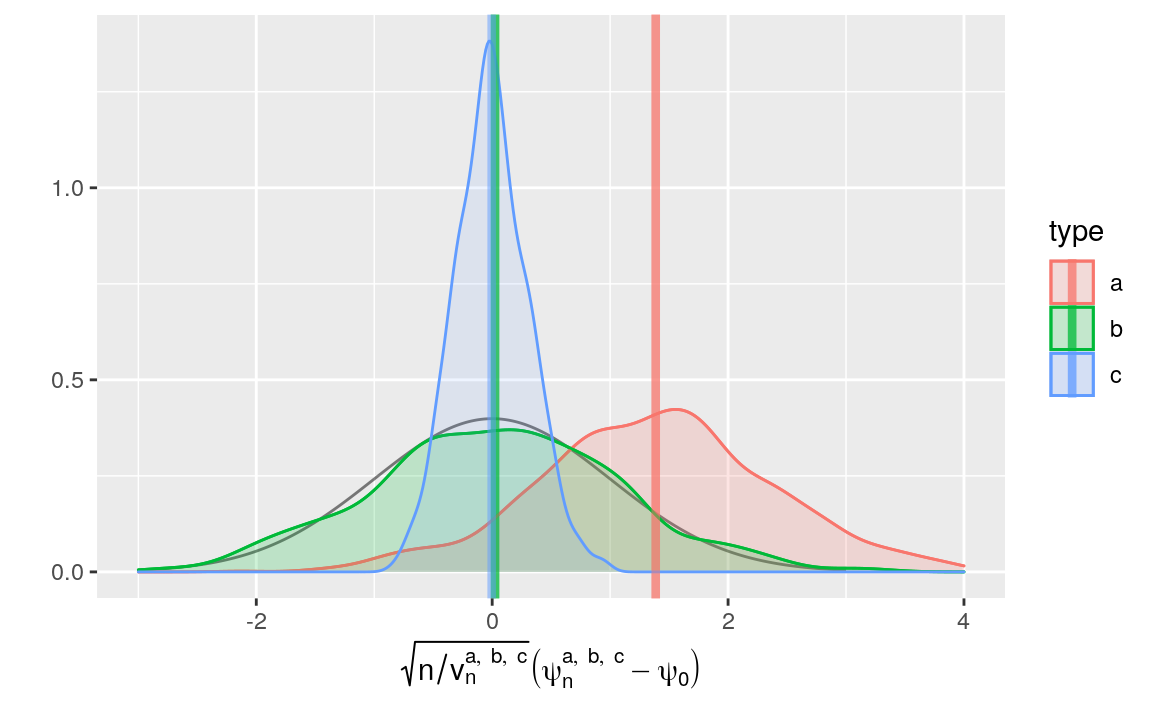
\includegraphics[width=0.7\linewidth]{img/unknown-Gbar-three-1} 

}

\caption{Kernel density estimators of the law of three estimators of \(\psi_{0}\) (recentered with respect to \(\psi_{0}\), and renormalized), one of them misconceived (a), one assuming that \(\Gbar_{0}\) is known (b) and one that hinges on the estimation of \(\Gbar_{0}\) (c). The present figure includes Figure \ref{fig:known-Gbar-one-b} (but the colors differ). Built based on 1000 independent realizations of each estimator.}\label{fig:unknown-Gbar-three}
\end{figure}



\begin{Shaded}
\begin{Highlighting}[]
\FunctionTok{ggplot}\NormalTok{(psi\_hat\_abc, }\FunctionTok{aes}\NormalTok{(}\AttributeTok{sample =}\NormalTok{ clt, }\AttributeTok{fill =}\NormalTok{ type, }\AttributeTok{colour =}\NormalTok{ type)) }\SpecialCharTok{+}
  \FunctionTok{geom\_abline}\NormalTok{(}\AttributeTok{intercept =} \DecValTok{0}\NormalTok{, }\AttributeTok{slope =} \DecValTok{1}\NormalTok{, }\AttributeTok{alpha =} \FloatTok{0.5}\NormalTok{) }\SpecialCharTok{+}
  \FunctionTok{geom\_qq}\NormalTok{(}\AttributeTok{alpha =} \DecValTok{1}\NormalTok{)}
\end{Highlighting}
\end{Shaded}

\begin{figure}

{\centering 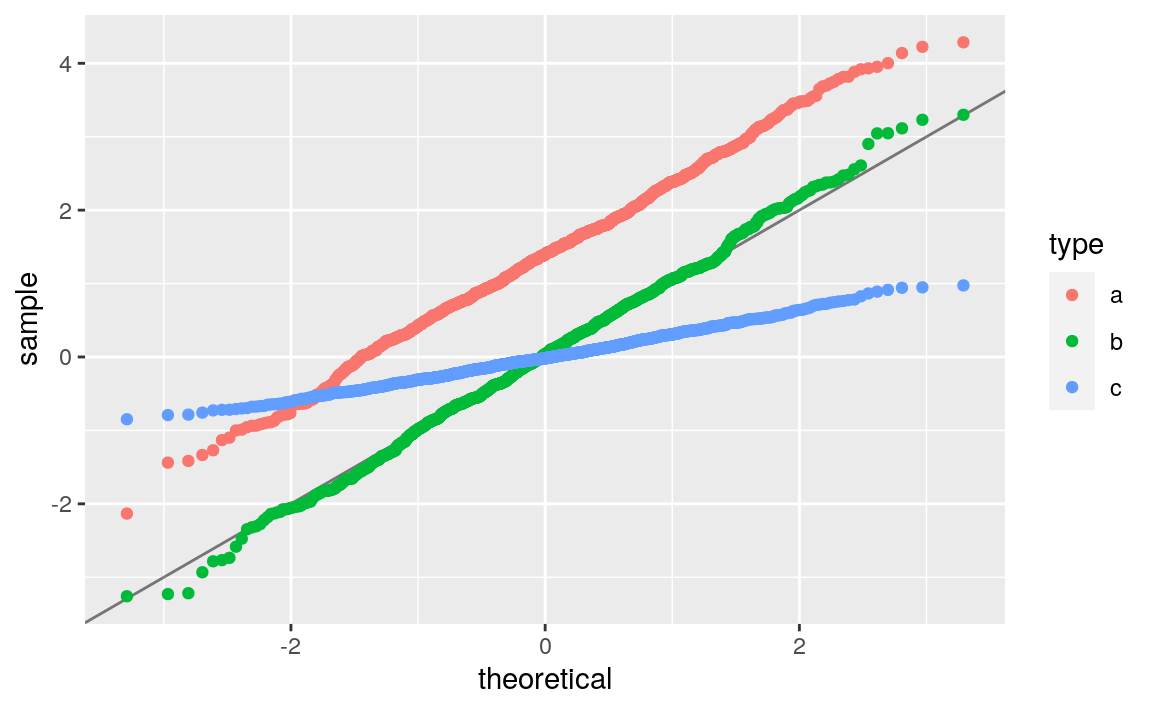
\includegraphics[width=0.7\linewidth]{img/unknown-Gbar-four-1} 

}

\caption{Quantile-quantile plot of the standard normal law against the empirical laws of three estimators of \(\psi_{0}\), one of them misconceived (a), one assuming that \(\Gbar_{0}\) is known (b) and one that hinges on the estimation of \(\Gbar_{0}\) (c). Built based on 1000 independent realizations of each estimator.}\label{fig:unknown-Gbar-four}
\end{figure}

Figures \ref{fig:unknown-Gbar-three} and \ref{fig:unknown-Gbar-four} confirm
that \(\psi_{n}^{c}\) behaves almost as well as \(\psi_{n}^{b}\) in terms of bias --- but
remember that we acted as oracles when we chose the well-specified algorithm
\(\Algo_{\Gbar,1}\). They also corroborate that \(v_{n}^{c}\), the estimator of
the asymptotic variance of \(\sqrt{n} (\psi_{n}^{c} - \psi_{0})\), is
conservative: for instance, the corresponding bell-shaped blue curve is too
much concentrated around its axis of symmetry.

The actual asymptotic variance of \(\sqrt{n} (\psi_{n}^{c} - \psi_{0})\) can be
estimated with the empirical variance of the 1000 replications of the
construction of \(\psi_{n}^{c}\).

\begin{Shaded}
\begin{Highlighting}[]
\NormalTok{(emp\_sig\_n }\OtherTok{\textless{}{-}}\NormalTok{ psi\_hat\_abc }\SpecialCharTok{\%\textgreater{}\%} \FunctionTok{filter}\NormalTok{(type }\SpecialCharTok{==} \StringTok{"c"}\NormalTok{) }\SpecialCharTok{\%\textgreater{}\%}
   \FunctionTok{summarize}\NormalTok{(}\FunctionTok{sd}\NormalTok{(psi\_n)) }\SpecialCharTok{\%\textgreater{}\%}\NormalTok{ pull)}
\CommentTok{\#\textgreater{} [1] 0.0172}
\NormalTok{(summ\_sig\_n }\OtherTok{\textless{}{-}}\NormalTok{ psi\_hat\_abc }\SpecialCharTok{\%\textgreater{}\%} \FunctionTok{filter}\NormalTok{(type }\SpecialCharTok{==} \StringTok{"c"}\NormalTok{) }\SpecialCharTok{\%\textgreater{}\%} \FunctionTok{select}\NormalTok{(sig\_n) }\SpecialCharTok{\%\textgreater{}\%}
\NormalTok{   summary)}
\CommentTok{\#\textgreater{}      sig\_n       }
\CommentTok{\#\textgreater{}  Min.   :0.0517  }
\CommentTok{\#\textgreater{}  1st Qu.:0.0549  }
\CommentTok{\#\textgreater{}  Median :0.0559  }
\CommentTok{\#\textgreater{}  Mean   :0.0560  }
\CommentTok{\#\textgreater{}  3rd Qu.:0.0570  }
\CommentTok{\#\textgreater{}  Max.   :0.0623}
\end{Highlighting}
\end{Shaded}

The empirical standard deviation is approximately
3.254 times smaller than the average
\emph{estimated} standard deviation. The estimator is conservative indeed!
Furthermore, note the better fit with the density of the standard normal
density of the kernel density estimator of the law of \(\sqrt{n} (\psi_{n}^{c} - \psi_{0})\) \textbf{renormalized with} \texttt{emp\_sig\_n}.



\begin{Shaded}
\begin{Highlighting}[]
\NormalTok{clt\_c }\OtherTok{\textless{}{-}}\NormalTok{ psi\_hat\_abc }\SpecialCharTok{\%\textgreater{}\%} \FunctionTok{filter}\NormalTok{(type }\SpecialCharTok{==} \StringTok{"c"}\NormalTok{) }\SpecialCharTok{\%\textgreater{}\%}
  \FunctionTok{mutate}\NormalTok{(}\AttributeTok{clt =}\NormalTok{ clt }\SpecialCharTok{*}\NormalTok{ sig\_n }\SpecialCharTok{/}\NormalTok{ emp\_sig\_n)}

\NormalTok{fig\_bias\_ab }\SpecialCharTok{+}
  \FunctionTok{geom\_density}\NormalTok{(}\FunctionTok{aes}\NormalTok{(clt, }\AttributeTok{fill =}\NormalTok{ type, }\AttributeTok{colour =}\NormalTok{ type), clt\_c, }\AttributeTok{alpha =} \FloatTok{0.1}\NormalTok{) }\SpecialCharTok{+}
  \FunctionTok{geom\_vline}\NormalTok{(}\FunctionTok{aes}\NormalTok{(}\AttributeTok{xintercept =}\NormalTok{ bias, }\AttributeTok{colour =}\NormalTok{ type),}
\NormalTok{             bias\_abc, }\AttributeTok{size =} \FloatTok{1.5}\NormalTok{, }\AttributeTok{alpha =} \FloatTok{0.5}\NormalTok{) }\SpecialCharTok{+}
  \FunctionTok{xlim}\NormalTok{(}\SpecialCharTok{{-}}\DecValTok{3}\NormalTok{, }\DecValTok{4}\NormalTok{) }\SpecialCharTok{+} 
  \FunctionTok{labs}\NormalTok{(}\AttributeTok{y =} \StringTok{""}\NormalTok{,}
       \AttributeTok{x =} \FunctionTok{bquote}\NormalTok{(}\FunctionTok{paste}\NormalTok{(}\FunctionTok{sqrt}\NormalTok{(n}\SpecialCharTok{/}\NormalTok{v[n]}\SpecialCharTok{\^{}}\NormalTok{\{}\FunctionTok{list}\NormalTok{(a, b, c)\})}\SpecialCharTok{*}
\NormalTok{                        (psi[n]}\SpecialCharTok{\^{}}\NormalTok{\{}\FunctionTok{list}\NormalTok{(a, b, c)\} }\SpecialCharTok{{-}}\NormalTok{ psi[}\DecValTok{0}\NormalTok{]))))}
\end{Highlighting}
\end{Shaded}

\begin{figure}

{\centering 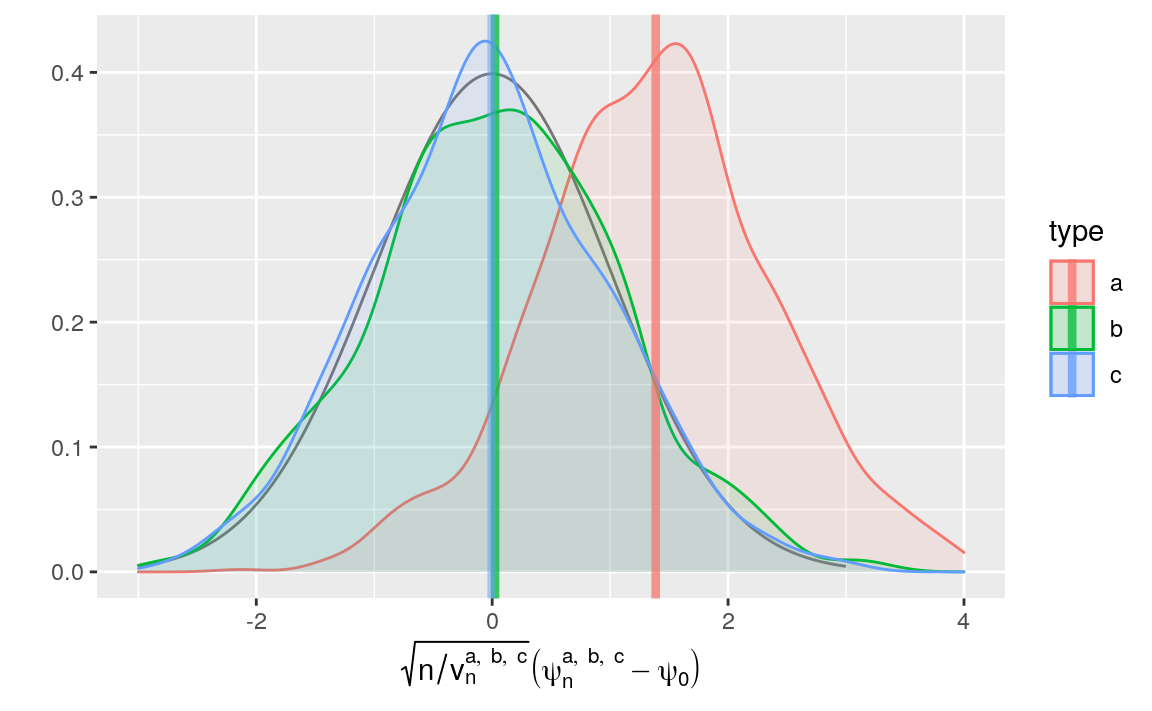
\includegraphics[width=0.7\linewidth]{img/unknown-Gbar-seven-1} 

}

\caption{Kernel density estimators of the law of three estimators of \(\psi_{0}\) (recentered with respect to \(\psi_{0}\), and renormalized), one of them misconceived (a), one assuming that \(\Gbar_{0}\) is known (b) and one that hinges on the estimation of \(\Gbar_{0}\) \textbf{and an estimator of the asymptotic variance computed across the replications} (c). The present figure includes Figure \ref{fig:known-Gbar-one-b} (but the colors differ) and it should be compared to Figure \ref{fig:unknown-Gbar-four}. Built based on 1000 independent realizations of each estimator.}\label{fig:unknown-Gbar-seven}
\end{figure}

\textbf{Workaround.} In a real world data-analysis, one could correct the
estimation of the asymptotic variance of \(\sqrt{n} (\psi_{n}^{c} - \psi_{0})\).
We could for instance derive the influence function as it is
described \protect\hyperlink{iptw-est-var}{there} in Appendix \ref{iptw-est-var} and use the
corresponding influence function-based estimator of the variance. One could
also rely on the cross-validation, possibly combined with the previous
workaround. Or one could also rely on the bootstrap.\footnote{That is, replicate the
  construction of \(\psi_{n}^{c}\) many times based on data sets obtained by
  resampling from the original data set, then estimate the asymptotic variance
  with the empirical variance of \(\psi_{n}^{c}\) computed across the
  replications.} This, however, would only make sense if one knew for sure that
the algorithm for the estimation of \(\Gbar_{0}\) is well-specified.

\hypertarget{exo-a-nice-title}{%
\section{\texorpdfstring{⚙ \gear Investigating further the IPTW inference strategy}{⚙ Investigating further the IPTW inference strategy}}\label{exo-a-nice-title}}

\begin{enumerate}
\def\labelenumi{\arabic{enumi}.}
\item
  Building upon the chunks of code devoted to the repeated computation of
  \(\psi_{n}^{b}\) and its companion quantities, construct confidence intervals
  for \(\psi_{0}\) of (asymptotic) level \(95\%\), and check if the empirical
  coverage is satisfactory. Note that if the coverage was exactly \(95\%\), then
  the number of confidence intervals that would contain \(\psi_{0}\) would follow
  a binomial law with parameters 1000 and \texttt{0.95}, and recall that function
  \texttt{binom.test} performs an exact test of a simple null hypothesis about the
  probability of success in a Bernoulli experiment against its three one-sided
  and two-sided alternatives.
\item
  Discuss what happens when the dimension of the (still well-specified)\index{well/mis-specified} working model grows. Start with the built-in working model \texttt{working\_model\_G\_two}. The following chunk of code re-defines \texttt{working\_model\_G\_two}
\end{enumerate}

\begin{Shaded}
\begin{Highlighting}[]
\DocumentationTok{\#\# make sure \textquotesingle{}1/2\textquotesingle{} and \textquotesingle{}1\textquotesingle{} belong to \textquotesingle{}powers\textquotesingle{}}
\NormalTok{powers }\OtherTok{\textless{}{-}} \FunctionTok{rep}\NormalTok{(}\FunctionTok{seq}\NormalTok{(}\DecValTok{1}\SpecialCharTok{/}\DecValTok{4}\NormalTok{, }\DecValTok{3}\NormalTok{, }\AttributeTok{by =} \DecValTok{1}\SpecialCharTok{/}\DecValTok{4}\NormalTok{), }\AttributeTok{each =} \DecValTok{2}\NormalTok{) }
\NormalTok{working\_model\_G\_two }\OtherTok{\textless{}{-}} \FunctionTok{list}\NormalTok{(}
  \AttributeTok{model =} \ControlFlowTok{function}\NormalTok{(...) \{}\FunctionTok{trim\_glm\_fit}\NormalTok{(}\FunctionTok{glm}\NormalTok{(}\AttributeTok{family =} \FunctionTok{binomial}\NormalTok{(), ...))\},}
  \AttributeTok{formula =}\NormalTok{ stats}\SpecialCharTok{::}\FunctionTok{as.formula}\NormalTok{(}
    \FunctionTok{paste}\NormalTok{(}\StringTok{"A \textasciitilde{}"}\NormalTok{,}
          \FunctionTok{paste}\NormalTok{(}\FunctionTok{c}\NormalTok{(}\StringTok{"I(W\^{}"}\NormalTok{, }\StringTok{"I(abs(W {-} 5/12)\^{}"}\NormalTok{),}
\NormalTok{                powers, }
                \AttributeTok{sep =} \StringTok{""}\NormalTok{, }\AttributeTok{collapse =} \StringTok{") + "}\NormalTok{),}
          \StringTok{")"}\NormalTok{)}
\NormalTok{  ),}
  \AttributeTok{type\_of\_preds =} \StringTok{"response"}
\NormalTok{)}
\FunctionTok{attr}\NormalTok{(working\_model\_G\_two, }\StringTok{"ML"}\NormalTok{) }\OtherTok{\textless{}{-}} \ConstantTok{FALSE}
\end{Highlighting}
\end{Shaded}

\begin{enumerate}
\def\labelenumi{\arabic{enumi}.}
\setcounter{enumi}{2}
\item
  Play around with argument \texttt{powers} (making sure that \texttt{1/2} and \texttt{1} belong to
  it), and plot graphics similar to those presented in Figures
  \ref{fig:unknown-Gbar-three} and \ref{fig:unknown-Gbar-four}.
\item
  Discuss what happens when the working model is
  mis-specified.\index{well/mis-specified} You could use the built-in working
  model \texttt{working\_model\_G\_three}.
\item
  Repeat the analysis developed in response to problem 1 above but for
  \(\psi_{n}^{c}\). What can you say about the coverage of the confidence
  intervals?
\item
  ☡ \stixdanger{} (Follow-up to problem 5). Implement the bootstrap
  procedure evoked at the end of Section \ref{empirical-inves-IPTW-bis}. Repeat
  the analysis developed in response to problem 1. Compare your results with
  those to problem 5.
\item
  ☡ \stixdanger{} Is it legitimate to infer the asymptotic variance
  of \(\psi_{n}^{c}\) with \(v_{n}^{c}\) when one relies on a very
  data-adaptive/versatile algorithm to estimate \(\Gbar_{0}\)?
\end{enumerate}

\hypertarget{Gcomp-estimator}{%
\section{G-computation estimator}\label{Gcomp-estimator}}

\hypertarget{Gcomp-construction}{%
\subsection{Construction and computation}\label{Gcomp-construction}}

Let \(\Algo_{Q_{W}}\) be an algorithm designed for the estimation of \(Q_{0,W}\)
(see Section \ref{nuisance-QW}). We denote by \(Q_{n,W} \defq \Algo_{Q_{W}}(P_{n})\) the output of the algorithm trained on \(P_{n}\).

Let \(\Algo_{\Qbar}\) be an algorithm designed for the estimation of \(\Qbar_{0}\)
(see Section \ref{nuisance-Qbar}). We denote by \(\Qbar_{n} \defq \Algo_{\Qbar}(P_{n})\) the output of the algorithm trained on \(P_{n}\).

Equation \eqref{eq:psi-zero} suggests the following, simple estimator of
\(\Psi(P_0)\):

\begin{equation} 
\psi_{n}   \defq   \int   \left(\Qbar_{n}(1,   w)   -   \Qbar_{n}(0,w)\right)
dQ_{n,W}(w). \label{eq:Gcomp-estimator}
\end{equation}

In words, this estimator is implemented by first regressing \(Y\) on \((A,W)\),
then by marginalizing with respect to the estimated law of \(W\). The resulting
estimator is referred to as a \emph{G-computation} (or \emph{standardization})
estimator.

From a computational point of view, the \texttt{tlrider} package makes it easy to
build the G-computation estimator. Recall that we have already estimated the
marginal law \(Q_{0,W}\) of \(W\) under \(P_{0}\) by training the algorithm
\(\Algo_{Q_{W}}\) as it is implemented in \texttt{estimate\_QW} on the \(n = 1000\) first
observations in \texttt{obs} (see Section \ref{nuisance-QW}):

\begin{Shaded}
\begin{Highlighting}[]
\NormalTok{QW\_hat }\OtherTok{\textless{}{-}} \FunctionTok{estimate\_QW}\NormalTok{(}\FunctionTok{head}\NormalTok{(obs, }\FloatTok{1e3}\NormalTok{))}
\end{Highlighting}
\end{Shaded}

Recall that \(\Algo_{\Qbar,1}\) is the algorithm for the estimation of
\(\Qbar_{0}\) as it is implemented in \texttt{estimate\_Qbar} with its argument
\texttt{algorithm} set to the built-in \texttt{working\_model\_Q\_one} (see Section
\ref{nuisance-Qbar-wm}). Recall also that \(\Algo_{\Qbar,\text{kNN}}\) is the
algorithm for the estimation of \(\Qbar_{0}\) as it is implemented in
\texttt{estimate\_Qbar} with its argument \texttt{algorithm} set to the built-in \texttt{kknn\_algo}
(see Section \ref{Qbar-knn-algo}). We have already trained the latter on the
\(n=1000\) first observations in \texttt{obs}. Let us train the former on the same data
set:

\begin{Shaded}
\begin{Highlighting}[]
\NormalTok{Qbar\_hat\_kknn }\OtherTok{\textless{}{-}} \FunctionTok{estimate\_Qbar}\NormalTok{(}\FunctionTok{head}\NormalTok{(obs, }\FloatTok{1e3}\NormalTok{),}
                               \AttributeTok{algorithm =}\NormalTok{ kknn\_algo,}
                               \AttributeTok{trControl =}\NormalTok{ kknn\_control,}
                               \AttributeTok{tuneGrid =}\NormalTok{ kknn\_grid)}
\end{Highlighting}
\end{Shaded}

\begin{Shaded}
\begin{Highlighting}[]
\NormalTok{Qbar\_hat\_d }\OtherTok{\textless{}{-}} \FunctionTok{estimate\_Qbar}\NormalTok{(}\FunctionTok{head}\NormalTok{(obs, }\FloatTok{1e3}\NormalTok{), working\_model\_Q\_one)}
\end{Highlighting}
\end{Shaded}

With these estimators handy, computing the G-computation estimator is as
simple as running the following chunk of code:

\begin{Shaded}
\begin{Highlighting}[]
\NormalTok{(}\FunctionTok{compute\_gcomp}\NormalTok{(QW\_hat, }\FunctionTok{wrapper}\NormalTok{(Qbar\_hat\_kknn, }\ConstantTok{FALSE}\NormalTok{), }\FloatTok{1e3}\NormalTok{))}
\CommentTok{\#\textgreater{} \# A tibble: 1 x 2}
\CommentTok{\#\textgreater{}   psi\_n   sig\_n}
\CommentTok{\#\textgreater{}   \textless{}dbl\textgreater{}   \textless{}dbl\textgreater{}}
\CommentTok{\#\textgreater{} 1 0.101 0.00306}
\NormalTok{(}\FunctionTok{compute\_gcomp}\NormalTok{(QW\_hat, }\FunctionTok{wrapper}\NormalTok{(Qbar\_hat\_d, }\ConstantTok{FALSE}\NormalTok{), }\FloatTok{1e3}\NormalTok{))}
\CommentTok{\#\textgreater{} \# A tibble: 1 x 2}
\CommentTok{\#\textgreater{}   psi\_n   sig\_n}
\CommentTok{\#\textgreater{}   \textless{}dbl\textgreater{}   \textless{}dbl\textgreater{}}
\CommentTok{\#\textgreater{} 1 0.109 0.00215}
\end{Highlighting}
\end{Shaded}

Note how we use function \texttt{wrapper} again, and that it is necessary to provide
the number of observations upon which the estimation of the \(Q_{W}\) and
\(\Qbar\) features of \(P_{0}\).

\hypertarget{elementary-statistical-properties-1}{%
\subsection{Elementary statistical properties}\label{elementary-statistical-properties-1}}

This subsection is very similar to its counterpart for the IPTW estimator, see
Section \ref{elementary-stat-prop-iptw}.

Let us denote by \(\Qbar_{n,1}\) the output of algorithm \(\Algo_{\Qbar,1}\)
trained on \(P_{n}\), and recall that \(\Qbar_{n,\text{kNN}}\) is the output of
algorithm \(\Algo_{\Qbar,\text{kNN}}\) trained on \(P_{n}\). Let \(\psi_{n}^{d}\)
and \(\psi_{n}^{e}\) be the G-computation estimators obtained by substituting
\(\Qbar_{n,1}\) and \(\Qbar_{n,\text{kNN}}\) for \(\Qbar_{n}\) in
\eqref{eq:Gcomp-estimator}, respectively.

If \(\Qbar_{n,\bullet}\) minimized the empirical risk over a
finite-dimensional, identifiable, and \textbf{well-specified} working model, then
\(\sqrt{n} (\psi_{n}^{\bullet} - \psi_{0})\) would converge in law to a
centered Gaussian law (here \(\psi_{n}^{\bullet}\) represents the G-computation
estimator obtained by substituting \(\Qbar_{n,\bullet}\) for \(\Qbar_{n}\) in
\eqref{eq:Gcomp-estimator}).\index{identifiability} Moreover, the asymptotic
variance of \(\sqrt{n} (\psi_{n}^{\bullet} - \psi_{0})\) would be estimated
\textbf{anti-conservatively}\footnote{In words, \(v_{n}^{d}\) converges to a lower-bound of
  the true asymptotic variance.}\index{conservative} with\index{well/mis-specified}

\begin{align} 
v_{n}^{d}            &\defq            \Var_{P_{n}}
\left(\Qbar_{n,1}(1,\cdot) - \Qbar_{n,1}(0,\cdot)\right) \\ &= \frac{1}{n}
\sum_{i=1}^{n}\left(\Qbar_{n,1}(1,W_{i})         -        \Qbar_{n,1}(0,W_{i})
-\psi_{n}^{d}\right)^{2}.  \label{eq:var-Gcomp-n} 
\end{align}

Unfortunately, algorithm \(\Algo_{\Qbar,1}\) is mis-specified and
\(\Algo_{\Qbar,\text{kNN}}\) is not based on a finite-dimensional working
model. Nevertheless, function \texttt{compute\_gcomp} estimates (in general, very
poorly) the asymptotic variance with \eqref{eq:var-Gcomp-n}.

We investigate \emph{empirically} the statistical behavior of \(\psi_{n}^{d}\) in
Section \ref{empirical-inves-Gcomp}. For an analysis of the reason why
\(v_{n}^{d}\) is an anti-conservative estimator of the asymptotic variance of
\(\sqrt{n} (\psi_{n}^{d} - \psi_{0})\), see \protect\hyperlink{gcomp-est-var}{there} in Appendix
\ref{gcomp-est-var}. We wish to emphasize that anti-conservativeness is even
more embarrassing that conservativeness (both being contingent on the fact
that the algorithms are well-specified, fact that cannot be true in the
present case in real world situations).

What would happen if we used a less amenable algorithm \(\Algo_{\Qbar}\). For
instance, \(\Algo_{\Qbar}\) could still be well-specified but so
\emph{versatile/complex} (as opposed to being based on well-behaved,
finite-dimensional parametric model) that the estimator \(\Qbar_{n}\), though
still consistent, would converge slowly to its target. Then, root-\(n\)
consistency would fail to hold. We can explore empirically this situation
with estimator \(\psi_{n}^{e}\) that hinges on algorithm
\(\Algo_{\Qbar,\text{kNN}}\). Or \(\Algo_{\Qbar}\) could be
mis-specified\index{well/mis-specified} and there would be no guarantee at all
that the resulting estimator \(\psi_{n}\) be even consistent.

\hypertarget{empirical-inves-Gcomp}{%
\subsection{Empirical investigation, fixed sample size}\label{empirical-inves-Gcomp}}

Let us compute \(\psi_{n}^{d}\) and \(\psi_{n}^{e}\) on the same \texttt{iter\ =}
1000 independent samples of independent observations drawn from \(P_{0}\) as in
Sections \ref{known-gbar-first-pass} and \ref{empirical-inves-IPTW-bis}. We
first enrich object \texttt{learned\_features\_fixed\_sample\_size} that was created in
Section \ref{empirical-inves-IPTW-bis}, adding to it estimators of
\(\Qbar_{0}\) obtained by training algorithms \(\Algo_{\Qbar,1}\) and
\(\Algo_{\Qbar,\text{kNN}}\) on each smaller data set.

The second series of commands creates object \texttt{psi\_hat\_de}, an 1000 by six
\texttt{tibble} containing notably the values of \(\psi_{n}^{d}\) and
\(\sqrt{v_{n}^{d}}/\sqrt{n}\) computed by calling \texttt{compute\_gcomp}, and those of
the recentered (with respect to \(\psi_{0}\)) and renormalized
\(\sqrt{n}/\sqrt{v_{n}^{d}} (\psi_{n}^{d} - \psi_{0})\). Because we know
beforehand that \(v_{n}^{d}\) under-estimates the actual asymptotic variance of
\(\sqrt{n} (\psi_{n}^{d} - \psi_{0})\), the \texttt{tibble} also includes the values of
\(\sqrt{n}/\sqrt{v^{d*}} (\psi_{n}^{d} - \psi_{0})\) where the estimator
\(v^{d*}\) of the asymptotic variance is computed \emph{across the replications of
\(\psi_{n}^{d}\)}. The tibble includes the same quantities pertaining to
\(\psi_{n}^{e}\), although there is no theoretical guarantee that the central
limit theorem does hold and, even if it did, that the counterpart \(v_{n}^{e}\)
to \(v_{n}^{d}\) estimates in any way the asymptotic variance of \(\sqrt{n} (\psi_{n}^{e} - \psi_{0})\).

Finally, \texttt{bias\_de} reports amounts of bias (at the renormalized scales ---
plural). There is one value of bias for each combination of \emph{(i)} type of the
estimator (\texttt{d} or \texttt{e}) and \emph{(ii)} how the renormalization is carried out,
either based on \(v_{n}^{d}\) and \(v_{n}^{e}\) (\texttt{auto\_renormalization} is \texttt{TRUE})
\emph{or} on the estimator of the asymptotic variance computed across the
replications of \(\psi_{n}^{d}\) and \(\psi_{n}^{e}\) (\texttt{auto\_renormalization} is
\texttt{FALSE}).



\begin{Shaded}
\begin{Highlighting}[]
\NormalTok{learned\_features\_fixed\_sample\_size }\OtherTok{\textless{}{-}}
\NormalTok{  learned\_features\_fixed\_sample\_size }\SpecialCharTok{\%\textgreater{}\%} 
  \FunctionTok{mutate}\NormalTok{(}\AttributeTok{Qbar\_hat\_d =}
           \FunctionTok{map}\NormalTok{(obs,}
               \SpecialCharTok{\textasciitilde{}} \FunctionTok{estimate\_Qbar}\NormalTok{(., }\AttributeTok{algorithm =}\NormalTok{ working\_model\_Q\_one)),}
         \AttributeTok{Qbar\_hat\_e =}
           \FunctionTok{map}\NormalTok{(obs,}
               \SpecialCharTok{\textasciitilde{}} \FunctionTok{estimate\_Qbar}\NormalTok{(., }\AttributeTok{algorithm =}\NormalTok{ kknn\_algo,}
                               \AttributeTok{trControl =}\NormalTok{ kknn\_control,}
                               \AttributeTok{tuneGrid =}\NormalTok{ kknn\_grid))) }\SpecialCharTok{\%\textgreater{}\%}
  \FunctionTok{mutate}\NormalTok{(}\AttributeTok{QW =} \FunctionTok{map}\NormalTok{(obs, estimate\_QW),}
         \AttributeTok{est\_d =}
           \FunctionTok{pmap}\NormalTok{(}\FunctionTok{list}\NormalTok{(QW, Qbar\_hat\_d, }\FunctionTok{n}\NormalTok{()),}
                \SpecialCharTok{\textasciitilde{}} \FunctionTok{compute\_gcomp}\NormalTok{(..}\DecValTok{1}\NormalTok{, }\FunctionTok{wrapper}\NormalTok{(..}\DecValTok{2}\NormalTok{, }\ConstantTok{FALSE}\NormalTok{), ..}\DecValTok{3}\NormalTok{)),}
         \AttributeTok{est\_e =}
           \FunctionTok{pmap}\NormalTok{(}\FunctionTok{list}\NormalTok{(QW, Qbar\_hat\_e, }\FunctionTok{n}\NormalTok{()),}
                \SpecialCharTok{\textasciitilde{}} \FunctionTok{compute\_gcomp}\NormalTok{(..}\DecValTok{1}\NormalTok{, }\FunctionTok{wrapper}\NormalTok{(..}\DecValTok{2}\NormalTok{, }\ConstantTok{FALSE}\NormalTok{), ..}\DecValTok{3}\NormalTok{)))}

\NormalTok{psi\_hat\_de }\OtherTok{\textless{}{-}}\NormalTok{ learned\_features\_fixed\_sample\_size }\SpecialCharTok{\%\textgreater{}\%}
  \FunctionTok{select}\NormalTok{(est\_d, est\_e) }\SpecialCharTok{\%\textgreater{}\%}
  \FunctionTok{pivot\_longer}\NormalTok{(}\FunctionTok{c}\NormalTok{(}\StringTok{\textasciigrave{}}\AttributeTok{est\_d}\StringTok{\textasciigrave{}}\NormalTok{, }\StringTok{\textasciigrave{}}\AttributeTok{est\_e}\StringTok{\textasciigrave{}}\NormalTok{),}
               \AttributeTok{names\_to =} \StringTok{"type"}\NormalTok{, }\AttributeTok{values\_to =} \StringTok{"estimates"}\NormalTok{) }\SpecialCharTok{\%\textgreater{}\%}
  \FunctionTok{extract}\NormalTok{(type, }\StringTok{"type"}\NormalTok{, }\StringTok{"\_([de])$"}\NormalTok{) }\SpecialCharTok{\%\textgreater{}\%} 
  \FunctionTok{unnest}\NormalTok{(estimates) }\SpecialCharTok{\%\textgreater{}\%}
  \FunctionTok{group\_by}\NormalTok{(type) }\SpecialCharTok{\%\textgreater{}\%}
  \FunctionTok{mutate}\NormalTok{(}\AttributeTok{sig\_alt =} \FunctionTok{sd}\NormalTok{(psi\_n)) }\SpecialCharTok{\%\textgreater{}\%}
  \FunctionTok{mutate}\NormalTok{(}\AttributeTok{clt\_ =}\NormalTok{ (psi\_n }\SpecialCharTok{{-}}\NormalTok{ psi\_zero) }\SpecialCharTok{/}\NormalTok{ sig\_n,}
         \AttributeTok{clt\_alt =}\NormalTok{ (psi\_n }\SpecialCharTok{{-}}\NormalTok{ psi\_zero) }\SpecialCharTok{/}\NormalTok{ sig\_alt) }\SpecialCharTok{\%\textgreater{}\%}
  \FunctionTok{pivot\_longer}\NormalTok{(}\FunctionTok{c}\NormalTok{(}\StringTok{\textasciigrave{}}\AttributeTok{clt\_}\StringTok{\textasciigrave{}}\NormalTok{, }\StringTok{\textasciigrave{}}\AttributeTok{clt\_alt}\StringTok{\textasciigrave{}}\NormalTok{),}
               \AttributeTok{names\_to =} \StringTok{"key"}\NormalTok{, }\AttributeTok{values\_to =} \StringTok{"clt"}\NormalTok{) }\SpecialCharTok{\%\textgreater{}\%}
  \FunctionTok{extract}\NormalTok{(key, }\StringTok{"key"}\NormalTok{, }\StringTok{"\_(.*)$"}\NormalTok{) }\SpecialCharTok{\%\textgreater{}\%}
  \FunctionTok{mutate}\NormalTok{(}\AttributeTok{key =} \FunctionTok{ifelse}\NormalTok{(key }\SpecialCharTok{==} \StringTok{""}\NormalTok{, }\ConstantTok{TRUE}\NormalTok{, }\ConstantTok{FALSE}\NormalTok{)) }\SpecialCharTok{\%\textgreater{}\%}
  \FunctionTok{rename}\NormalTok{(}\StringTok{"auto\_renormalization"} \OtherTok{=}\NormalTok{ key)}

\NormalTok{(bias\_de }\OtherTok{\textless{}{-}}\NormalTok{ psi\_hat\_de }\SpecialCharTok{\%\textgreater{}\%}
   \FunctionTok{group\_by}\NormalTok{(type, auto\_renormalization) }\SpecialCharTok{\%\textgreater{}\%}
   \FunctionTok{summarize}\NormalTok{(}\AttributeTok{bias =} \FunctionTok{mean}\NormalTok{(clt), }\AttributeTok{.groups =} \StringTok{"drop"}\NormalTok{))}
\CommentTok{\#\textgreater{} \# A tibble: 4 x 3}
\CommentTok{\#\textgreater{}   type  auto\_renormalization  bias}
\CommentTok{\#\textgreater{}   \textless{}chr\textgreater{} \textless{}lgl\textgreater{}                \textless{}dbl\textgreater{}}
\CommentTok{\#\textgreater{} 1 d     FALSE                0.234}
\CommentTok{\#\textgreater{} 2 d     TRUE                 2.04 }
\CommentTok{\#\textgreater{} 3 e     FALSE                0.107}
\CommentTok{\#\textgreater{} 4 e     TRUE                 0.626}

\NormalTok{fig }\OtherTok{\textless{}{-}} \FunctionTok{ggplot}\NormalTok{() }\SpecialCharTok{+}
  \FunctionTok{geom\_line}\NormalTok{(}\FunctionTok{aes}\NormalTok{(}\AttributeTok{x =}\NormalTok{ x, }\AttributeTok{y =}\NormalTok{ y), }
            \AttributeTok{data =} \FunctionTok{tibble}\NormalTok{(}\AttributeTok{x =} \FunctionTok{seq}\NormalTok{(}\SpecialCharTok{{-}}\DecValTok{4}\NormalTok{, }\DecValTok{4}\NormalTok{, }\AttributeTok{length.out =} \FloatTok{1e3}\NormalTok{),}
                          \AttributeTok{y =} \FunctionTok{dnorm}\NormalTok{(x)),}
            \AttributeTok{linetype =} \DecValTok{1}\NormalTok{, }\AttributeTok{alpha =} \FloatTok{0.5}\NormalTok{) }\SpecialCharTok{+}
  \FunctionTok{geom\_density}\NormalTok{(}\FunctionTok{aes}\NormalTok{(clt, }\AttributeTok{fill =}\NormalTok{ type, }\AttributeTok{colour =}\NormalTok{ type),}
\NormalTok{               psi\_hat\_de, }\AttributeTok{alpha =} \FloatTok{0.1}\NormalTok{) }\SpecialCharTok{+}
  \FunctionTok{geom\_vline}\NormalTok{(}\FunctionTok{aes}\NormalTok{(}\AttributeTok{xintercept =}\NormalTok{ bias, }\AttributeTok{colour =}\NormalTok{ type),}
\NormalTok{             bias\_de, }\AttributeTok{size =} \FloatTok{1.5}\NormalTok{, }\AttributeTok{alpha =} \FloatTok{0.5}\NormalTok{) }\SpecialCharTok{+}
  \FunctionTok{facet\_wrap}\NormalTok{(}\SpecialCharTok{\textasciitilde{}}\NormalTok{ auto\_renormalization,}
             \AttributeTok{labeller =}
               \FunctionTok{as\_labeller}\NormalTok{(}\FunctionTok{c}\NormalTok{(}\StringTok{\textasciigrave{}}\AttributeTok{TRUE}\StringTok{\textasciigrave{}} \OtherTok{=} \StringTok{"auto{-}renormalization: TRUE"}\NormalTok{,}
                             \StringTok{\textasciigrave{}}\AttributeTok{FALSE}\StringTok{\textasciigrave{}} \OtherTok{=} \StringTok{"auto{-}renormalization: FALSE"}\NormalTok{)),}
             \AttributeTok{scales =} \StringTok{"free"}\NormalTok{)}
  
\NormalTok{fig }\SpecialCharTok{+}
  \FunctionTok{labs}\NormalTok{(}\AttributeTok{y =} \StringTok{""}\NormalTok{,}
       \AttributeTok{x =} \FunctionTok{bquote}\NormalTok{(}\FunctionTok{paste}\NormalTok{(}\FunctionTok{sqrt}\NormalTok{(n}\SpecialCharTok{/}\NormalTok{v[n]}\SpecialCharTok{\^{}}\NormalTok{\{}\FunctionTok{list}\NormalTok{(d, e)\})}\SpecialCharTok{*}
\NormalTok{                        (psi[n]}\SpecialCharTok{\^{}}\NormalTok{\{}\FunctionTok{list}\NormalTok{(d, e)\} }\SpecialCharTok{{-}}\NormalTok{ psi[}\DecValTok{0}\NormalTok{]))))}
\end{Highlighting}
\end{Shaded}

\begin{figure}

{\centering 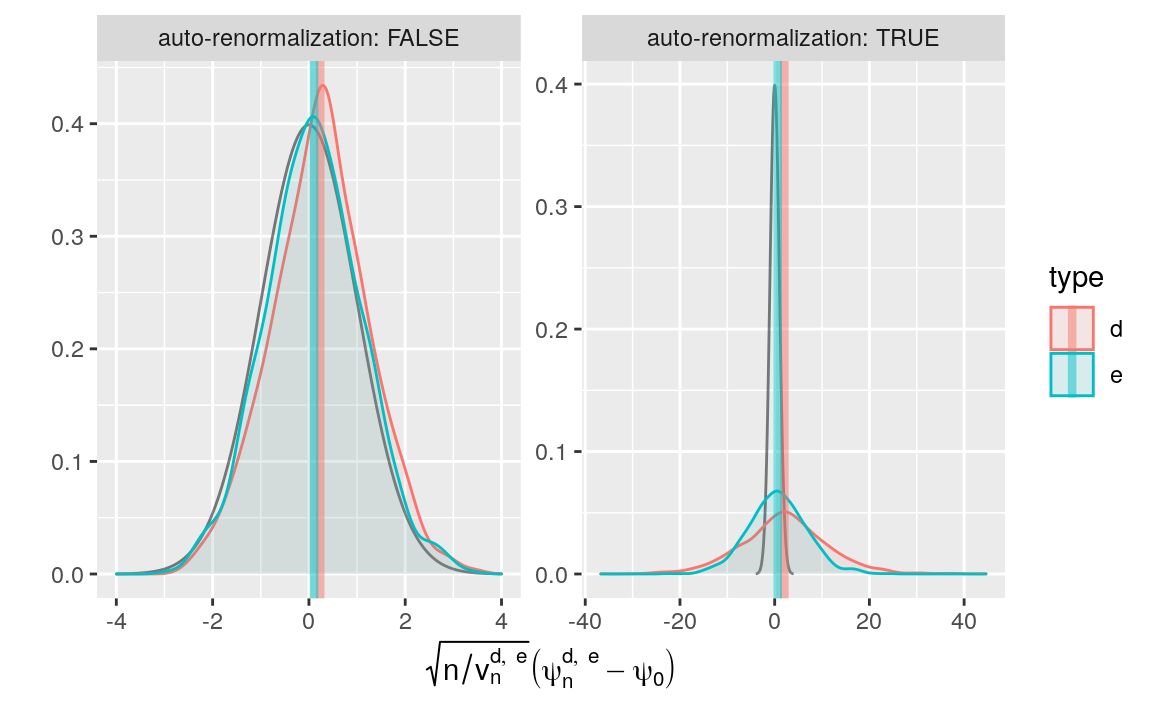
\includegraphics[width=0.7\linewidth]{img/estimating-Qbar-one-bis-1} 

}

\caption{Kernel density estimators of the law of two G-computation estimators of \(\psi_{0}\) (recentered with respect to \(\psi_{0}\), and renormalized). The estimators respectively hinge on algorithms \(\Algo_{\Qbar,1}\) (d) and \(\Algo_{\Qbar,\text{kNN}}\) (e) to estimate \(\Qbar_{0}\). Two renormalization schemes are considered, either based on an estimator of the asymptotic variance (right) or on the empirical variance computed across the 1000 independent replications of the estimators (left). We emphasize that the \(x\)-axis ranges differ between the left and right plots.}\label{fig:estimating-Qbar-one-bis}
\end{figure}

We represent the empirical laws of the recentered (with respect to \(\psi_{0}\)) and renormalized \(\psi_{n}^{d}\) and \(\psi_{n}^{e}\) in Figure \ref{fig:estimating-Qbar-one-bis} (kernel density estimators). Two renormalization schemes are considered, either based on an estimator of the asymptotic variance (left) or on the empirical variance computed across the 1000 independent replications of the estimators (right). We emphasize that the \(x\)-axis ranges differ between the left and right plots.

Two important comments are in order. First, on the one hand, the
G-computation estimator \(\psi_{n}^{d}\) is biased. Specifically, by the above
chunk of code, the averages of \(\sqrt{n/v_{n}^{d}} (\psi_{n}^{d} - \psi_{0})\)
and \(\sqrt{n/v_{n}^{d*}} (\psi_{n}^{d} - \psi_{0})\) computed across the
realizations are equal to 2.038 and 0.234 (see \texttt{bias\_de}). On the other hand, the G-computation
estimator \(\psi_{n}^{e}\) is biased too, though slightly less than
\(\psi_{n}^{d}\). Specifically, by the above chunk of code, the averages of
\(\sqrt{n/v_{n}^{e}} (\psi_{n}^{e} - \psi_{0})\) and \(\sqrt{n/v^{e*}} (\psi_{n}^{e} - \psi_{0})\) computed across the realizations are equal to
0.626 and 0.107 (see
\texttt{bias\_de}). We can provide an oracular explanation. Estimator \(\psi_{n}^{d}\)
suffers from the poor approximation of \(\Qbar_{0}\) by
\(\Algo_{\Qbar,1}(P_{n})\), a result of the algorithm's mis-specification. As
for \(\psi_{n}^{e}\), it behaves better because \(\Algo_{\Qbar,\text{kNN}} (P_{n})\) approximates \(\Qbar_{0}\) better than \(\Algo_{\Qbar,1}(P_{n})\), an
apparent consequence of the greater versatility of the algorithm.

Second, we get a visual confirmation that \(v_{n}^{d}\) under-estimates the
actual asymptotic variance of \(\sqrt{n} (\psi_{n}^{d} - \psi_{0})\): the
right-hand side red bell-shaped curve is too dispersed. In contrast, the
right-hand side blue bell-shaped curve is much closer to the black curve that
represents the density of the standard normal law. Looking at the left-hand
side plot reveals that the empirical law of \(\sqrt{n/v^{d*}} (\psi_{n}^{d} - \psi_{0})\), once translated to compensate for the bias, is rather close to the
black curve. This means that the random variable is approximately distributed
like a Gaussian random variable. On the contrary, the empirical law of
\(\sqrt{n/v^{e*}} (\psi_{n}^{e} - \psi_{0})\) does not strike us as being as
closely Gaussian-like as that of \(\sqrt{n/v^{d*}} (\psi_{n}^{d} - \psi_{0})\).
By being more data-adaptive than \(\Algo_{\Qbar,1}\), algorithm
\(\Algo_{\Qbar,\text{kNN}}\) yields a better estimator of \(\Qbar_{0}\). However,
the rate of convergence of \(\Algo_{\Qbar,\text{kNN}}(P_{n})\) to its limit may
be slower than root-\(n\), invalidating a central limit theorem.

How do the estimated variances of \(\psi_{n}^{d}\) and \(\psi_{n}^{e}\) compare
with their empirical counterparts (computed across the 1000 replications of
the construction of the two estimators)?

\begin{Shaded}
\begin{Highlighting}[]
\DocumentationTok{\#\# psi\_n\^{}d}
\NormalTok{(psi\_hat\_de }\SpecialCharTok{\%\textgreater{}\%}\NormalTok{ ungroup }\SpecialCharTok{\%\textgreater{}\%}
   \FunctionTok{filter}\NormalTok{(type }\SpecialCharTok{==} \StringTok{"d"} \SpecialCharTok{\&}\NormalTok{ auto\_renormalization) }\SpecialCharTok{\%\textgreater{}\%} \FunctionTok{pull}\NormalTok{(sig\_n) }\SpecialCharTok{\%\textgreater{}\%}\NormalTok{ summary)}
\CommentTok{\#\textgreater{}    Min. 1st Qu.  Median    Mean 3rd Qu.    Max. }
\CommentTok{\#\textgreater{} 0.00019 0.00169 0.00205 0.00206 0.00241 0.00369}
\DocumentationTok{\#\# psi\_n\^{}e}
\NormalTok{(psi\_hat\_de }\SpecialCharTok{\%\textgreater{}\%}\NormalTok{ ungroup }\SpecialCharTok{\%\textgreater{}\%}
   \FunctionTok{filter}\NormalTok{(type }\SpecialCharTok{==} \StringTok{"e"} \SpecialCharTok{\&}\NormalTok{ auto\_renormalization) }\SpecialCharTok{\%\textgreater{}\%} \FunctionTok{pull}\NormalTok{(sig\_n) }\SpecialCharTok{\%\textgreater{}\%}\NormalTok{ summary)}
\CommentTok{\#\textgreater{}    Min. 1st Qu.  Median    Mean 3rd Qu.    Max. }
\CommentTok{\#\textgreater{} 0.00170 0.00261 0.00287 0.00288 0.00314 0.00421}
\end{Highlighting}
\end{Shaded}

The empirical standard deviation of \(\psi_{n}^{d}\) is approximately
8.307 times larger than the average \emph{estimated}
standard deviation. The estimator is anti-conservative indeed!

As for the empirical standard deviation of \(\psi_{n}^{e}\), it is approximately
5.962 times larger than the average \emph{estimated}
standard deviation.

\hypertarget{empirical-inves-Gcomp-varying}{%
\subsection{\texorpdfstring{☡ \stixdanger{} Empirical investigation, varying sample size}{☡  Empirical investigation, varying sample size}}\label{empirical-inves-Gcomp-varying}}

\begin{Shaded}
\begin{Highlighting}[]
\NormalTok{sample\_size }\OtherTok{\textless{}{-}} \FunctionTok{c}\NormalTok{(}\DecValTok{2500}\NormalTok{, }\DecValTok{5000}\NormalTok{) }\CommentTok{\# 5e3, 15e3}
\NormalTok{block\_size }\OtherTok{\textless{}{-}} \FunctionTok{sum}\NormalTok{(sample\_size)}


\NormalTok{learned\_features\_varying\_sample\_size }\OtherTok{\textless{}{-}}\NormalTok{ obs }\SpecialCharTok{\%\textgreater{}\%}\NormalTok{ as\_tibble }\SpecialCharTok{\%\textgreater{}\%} 
  \FunctionTok{head}\NormalTok{(}\AttributeTok{n =}\NormalTok{ (}\FunctionTok{nrow}\NormalTok{(.) }\SpecialCharTok{\%/\%}\NormalTok{ block\_size) }\SpecialCharTok{*}\NormalTok{ block\_size) }\SpecialCharTok{\%\textgreater{}\%} 
  \FunctionTok{mutate}\NormalTok{(}\AttributeTok{block =} \FunctionTok{label}\NormalTok{(}\DecValTok{1}\SpecialCharTok{:}\FunctionTok{nrow}\NormalTok{(.), sample\_size)) }\SpecialCharTok{\%\textgreater{}\%}
  \FunctionTok{nest}\NormalTok{(}\AttributeTok{obs =} \FunctionTok{c}\NormalTok{(W, A, Y))}
\end{Highlighting}
\end{Shaded}

First, we cut the data set into independent sub-data sets of sample size \(n\)
in \(\{\) 2500, 5000 \(\}\). Second, we infer \(\psi_{0}\)
as shown two chunks earlier. We thus obtain 133
independent realizations of each estimator derived on data sets of \texttt{r\ length(sample\_size)}, increasing sample sizes.

\begin{Shaded}
\begin{Highlighting}[]
\NormalTok{learned\_features\_varying\_sample\_size }\OtherTok{\textless{}{-}}
\NormalTok{  learned\_features\_varying\_sample\_size }\SpecialCharTok{\%\textgreater{}\%}
  \FunctionTok{mutate}\NormalTok{(}\AttributeTok{Qbar\_hat\_d =}
           \FunctionTok{map}\NormalTok{(obs,}
               \SpecialCharTok{\textasciitilde{}} \FunctionTok{estimate\_Qbar}\NormalTok{(., }\AttributeTok{algorithm =}\NormalTok{ working\_model\_Q\_one)),}
         \AttributeTok{Qbar\_hat\_e =}
           \FunctionTok{map}\NormalTok{(obs,}
               \SpecialCharTok{\textasciitilde{}} \FunctionTok{estimate\_Qbar}\NormalTok{(., }\AttributeTok{algorithm =}\NormalTok{ kknn\_algo,}
                               \AttributeTok{trControl =}\NormalTok{ kknn\_control,}
                               \AttributeTok{tuneGrid =}\NormalTok{ kknn\_grid))) }\SpecialCharTok{\%\textgreater{}\%}
  \FunctionTok{mutate}\NormalTok{(}\AttributeTok{QW =} \FunctionTok{map}\NormalTok{(obs, estimate\_QW),}
         \AttributeTok{est\_d =}
           \FunctionTok{pmap}\NormalTok{(}\FunctionTok{list}\NormalTok{(QW, Qbar\_hat\_d, }\FunctionTok{n}\NormalTok{()),}
                \SpecialCharTok{\textasciitilde{}} \FunctionTok{compute\_gcomp}\NormalTok{(..}\DecValTok{1}\NormalTok{, }\FunctionTok{wrapper}\NormalTok{(..}\DecValTok{2}\NormalTok{, }\ConstantTok{FALSE}\NormalTok{), ..}\DecValTok{3}\NormalTok{)),}
         \AttributeTok{est\_e =}
           \FunctionTok{pmap}\NormalTok{(}\FunctionTok{list}\NormalTok{(QW, Qbar\_hat\_e, }\FunctionTok{n}\NormalTok{()),}
                \SpecialCharTok{\textasciitilde{}} \FunctionTok{compute\_gcomp}\NormalTok{(..}\DecValTok{1}\NormalTok{, }\FunctionTok{wrapper}\NormalTok{(..}\DecValTok{2}\NormalTok{, }\ConstantTok{FALSE}\NormalTok{), ..}\DecValTok{3}\NormalTok{)))}

\NormalTok{root\_n\_bias }\OtherTok{\textless{}{-}}\NormalTok{ learned\_features\_varying\_sample\_size }\SpecialCharTok{\%\textgreater{}\%}
  \FunctionTok{mutate}\NormalTok{(}\AttributeTok{block =} \FunctionTok{unlist}\NormalTok{(}\FunctionTok{map}\NormalTok{(}\FunctionTok{strsplit}\NormalTok{(block, }\StringTok{"\_"}\NormalTok{), }\SpecialCharTok{\textasciitilde{}}\NormalTok{.x[}\DecValTok{2}\NormalTok{])),}
         \AttributeTok{sample\_size =}\NormalTok{ sample\_size[}\FunctionTok{as.integer}\NormalTok{(block)]) }\SpecialCharTok{\%\textgreater{}\%}
  \FunctionTok{select}\NormalTok{(block, sample\_size, est\_d, est\_e) }\SpecialCharTok{\%\textgreater{}\%}
  \FunctionTok{pivot\_longer}\NormalTok{(}\FunctionTok{c}\NormalTok{(}\StringTok{\textasciigrave{}}\AttributeTok{est\_d}\StringTok{\textasciigrave{}}\NormalTok{, }\StringTok{\textasciigrave{}}\AttributeTok{est\_e}\StringTok{\textasciigrave{}}\NormalTok{),}
               \AttributeTok{names\_to =} \StringTok{"type"}\NormalTok{, }\AttributeTok{values\_to =} \StringTok{"estimates"}\NormalTok{) }\SpecialCharTok{\%\textgreater{}\%}
  \FunctionTok{extract}\NormalTok{(type, }\StringTok{"type"}\NormalTok{, }\StringTok{"\_([de])$"}\NormalTok{) }\SpecialCharTok{\%\textgreater{}\%} 
  \FunctionTok{unnest}\NormalTok{(estimates) }\SpecialCharTok{\%\textgreater{}\%}
  \FunctionTok{group\_by}\NormalTok{(block, type) }\SpecialCharTok{\%\textgreater{}\%}
  \FunctionTok{mutate}\NormalTok{(}\AttributeTok{sig\_alt =} \FunctionTok{sd}\NormalTok{(psi\_n)) }\SpecialCharTok{\%\textgreater{}\%}
  \FunctionTok{mutate}\NormalTok{(}\AttributeTok{clt\_ =}\NormalTok{ (psi\_n }\SpecialCharTok{{-}}\NormalTok{ psi\_zero) }\SpecialCharTok{/}\NormalTok{ sig\_n,}
         \AttributeTok{clt\_alt =}\NormalTok{ (psi\_n }\SpecialCharTok{{-}}\NormalTok{ psi\_zero) }\SpecialCharTok{/}\NormalTok{ sig\_alt) }\SpecialCharTok{\%\textgreater{}\%}
  \FunctionTok{pivot\_longer}\NormalTok{(}\FunctionTok{c}\NormalTok{(}\StringTok{\textasciigrave{}}\AttributeTok{clt\_}\StringTok{\textasciigrave{}}\NormalTok{, }\StringTok{\textasciigrave{}}\AttributeTok{clt\_alt}\StringTok{\textasciigrave{}}\NormalTok{),}
               \AttributeTok{names\_to =} \StringTok{"key"}\NormalTok{, }\AttributeTok{values\_to =} \StringTok{"clt"}\NormalTok{) }\SpecialCharTok{\%\textgreater{}\%}
  \FunctionTok{extract}\NormalTok{(key, }\StringTok{"key"}\NormalTok{, }\StringTok{"\_(.*)$"}\NormalTok{) }\SpecialCharTok{\%\textgreater{}\%}
  \FunctionTok{mutate}\NormalTok{(}\AttributeTok{key =} \FunctionTok{ifelse}\NormalTok{(key }\SpecialCharTok{==} \StringTok{""}\NormalTok{, }\ConstantTok{TRUE}\NormalTok{, }\ConstantTok{FALSE}\NormalTok{)) }\SpecialCharTok{\%\textgreater{}\%}
  \FunctionTok{rename}\NormalTok{(}\StringTok{"auto\_renormalization"} \OtherTok{=}\NormalTok{ key)}
\end{Highlighting}
\end{Shaded}

The \texttt{tibble} called \texttt{root\_n\_bias} reports root-\(n\) times bias for all
combinations of estimator and sample size. The next chunk of code presents
visually our findings, see Figure \ref{fig:estimating-Qbar-four}. Note how we
include the realizations of the estimators derived earlier and contained in
\texttt{psi\_hat\_de} (thus breaking the independence between components of
\texttt{root\_n\_bias}, a small price to pay in this context).



\begin{Shaded}
\begin{Highlighting}[]
\NormalTok{root\_n\_bias }\OtherTok{\textless{}{-}}\NormalTok{ learned\_features\_fixed\_sample\_size }\SpecialCharTok{\%\textgreater{}\%}
   \FunctionTok{mutate}\NormalTok{(}\AttributeTok{block =} \StringTok{"0"}\NormalTok{,}
          \AttributeTok{sample\_size =}\NormalTok{ B}\SpecialCharTok{/}\NormalTok{iter) }\SpecialCharTok{\%\textgreater{}\%}  \CommentTok{\# because *fixed* sample size}
   \FunctionTok{select}\NormalTok{(block, sample\_size, est\_d, est\_e) }\SpecialCharTok{\%\textgreater{}\%}
  \FunctionTok{pivot\_longer}\NormalTok{(}\FunctionTok{c}\NormalTok{(}\StringTok{\textasciigrave{}}\AttributeTok{est\_d}\StringTok{\textasciigrave{}}\NormalTok{, }\StringTok{\textasciigrave{}}\AttributeTok{est\_e}\StringTok{\textasciigrave{}}\NormalTok{),}
               \AttributeTok{names\_to =} \StringTok{"type"}\NormalTok{, }\AttributeTok{values\_to =} \StringTok{"estimates"}\NormalTok{) }\SpecialCharTok{\%\textgreater{}\%}
   \FunctionTok{extract}\NormalTok{(type, }\StringTok{"type"}\NormalTok{, }\StringTok{"\_([de])$"}\NormalTok{) }\SpecialCharTok{\%\textgreater{}\%} 
   \FunctionTok{unnest}\NormalTok{(estimates) }\SpecialCharTok{\%\textgreater{}\%}
   \FunctionTok{group\_by}\NormalTok{(block, type) }\SpecialCharTok{\%\textgreater{}\%}
   \FunctionTok{mutate}\NormalTok{(}\AttributeTok{sig\_alt =} \FunctionTok{sd}\NormalTok{(psi\_n)) }\SpecialCharTok{\%\textgreater{}\%}
   \FunctionTok{mutate}\NormalTok{(}\AttributeTok{clt\_ =}\NormalTok{ (psi\_n }\SpecialCharTok{{-}}\NormalTok{ psi\_zero) }\SpecialCharTok{/}\NormalTok{ sig\_n,}
          \AttributeTok{clt\_alt =}\NormalTok{ (psi\_n }\SpecialCharTok{{-}}\NormalTok{ psi\_zero) }\SpecialCharTok{/}\NormalTok{ sig\_alt) }\SpecialCharTok{\%\textgreater{}\%}
  \FunctionTok{pivot\_longer}\NormalTok{(}\FunctionTok{c}\NormalTok{(}\StringTok{\textasciigrave{}}\AttributeTok{clt\_}\StringTok{\textasciigrave{}}\NormalTok{, }\StringTok{\textasciigrave{}}\AttributeTok{clt\_alt}\StringTok{\textasciigrave{}}\NormalTok{),}
               \AttributeTok{names\_to =} \StringTok{"key"}\NormalTok{, }\AttributeTok{values\_to =} \StringTok{"clt"}\NormalTok{) }\SpecialCharTok{\%\textgreater{}\%}
   \FunctionTok{extract}\NormalTok{(key, }\StringTok{"key"}\NormalTok{, }\StringTok{"\_(.*)$"}\NormalTok{) }\SpecialCharTok{\%\textgreater{}\%}
   \FunctionTok{mutate}\NormalTok{(}\AttributeTok{key =} \FunctionTok{ifelse}\NormalTok{(key }\SpecialCharTok{==} \StringTok{""}\NormalTok{, }\ConstantTok{TRUE}\NormalTok{, }\ConstantTok{FALSE}\NormalTok{)) }\SpecialCharTok{\%\textgreater{}\%}
   \FunctionTok{rename}\NormalTok{(}\StringTok{"auto\_renormalization"} \OtherTok{=}\NormalTok{ key) }\SpecialCharTok{\%\textgreater{}\%}
   \FunctionTok{full\_join}\NormalTok{(root\_n\_bias)}
 
\NormalTok{root\_n\_bias }\SpecialCharTok{\%\textgreater{}\%} \FunctionTok{filter}\NormalTok{(auto\_renormalization) }\SpecialCharTok{\%\textgreater{}\%}
  \FunctionTok{mutate}\NormalTok{(}\AttributeTok{rnb =} \FunctionTok{sqrt}\NormalTok{(sample\_size) }\SpecialCharTok{*}\NormalTok{ (psi\_n }\SpecialCharTok{{-}}\NormalTok{ psi\_zero)) }\SpecialCharTok{\%\textgreater{}\%}
  \FunctionTok{group\_by}\NormalTok{(sample\_size, type) }\SpecialCharTok{\%\textgreater{}\%}
  \FunctionTok{ggplot}\NormalTok{() }\SpecialCharTok{+}
  \FunctionTok{stat\_summary}\NormalTok{(}\FunctionTok{aes}\NormalTok{(}\AttributeTok{x =}\NormalTok{ sample\_size, }\AttributeTok{y =}\NormalTok{ rnb,}
                   \AttributeTok{group =} \FunctionTok{interaction}\NormalTok{(sample\_size, type),}
                   \AttributeTok{color =}\NormalTok{ type),}
               \AttributeTok{fun.data =}\NormalTok{ mean\_se, }\AttributeTok{fun.args =} \FunctionTok{list}\NormalTok{(}\AttributeTok{mult =} \DecValTok{1}\NormalTok{),}
               \AttributeTok{position =} \FunctionTok{position\_dodge}\NormalTok{(}\AttributeTok{width =} \DecValTok{250}\NormalTok{), }\AttributeTok{cex =} \DecValTok{1}\NormalTok{) }\SpecialCharTok{+}
  \FunctionTok{stat\_summary}\NormalTok{(}\FunctionTok{aes}\NormalTok{(}\AttributeTok{x =}\NormalTok{ sample\_size, }\AttributeTok{y =}\NormalTok{ rnb,}
                   \AttributeTok{group =} \FunctionTok{interaction}\NormalTok{(sample\_size, type),}
                   \AttributeTok{color =}\NormalTok{ type),}
               \AttributeTok{fun.data =}\NormalTok{ mean\_se, }\AttributeTok{fun.args =} \FunctionTok{list}\NormalTok{(}\AttributeTok{mult =} \DecValTok{1}\NormalTok{),}
               \AttributeTok{position =} \FunctionTok{position\_dodge}\NormalTok{(}\AttributeTok{width =} \DecValTok{250}\NormalTok{), }\AttributeTok{cex =} \DecValTok{1}\NormalTok{,}
               \AttributeTok{geom =} \StringTok{"errorbar"}\NormalTok{, }\AttributeTok{width =} \DecValTok{750}\NormalTok{) }\SpecialCharTok{+}
  \FunctionTok{stat\_summary}\NormalTok{(}\FunctionTok{aes}\NormalTok{(}\AttributeTok{x =}\NormalTok{ sample\_size, }\AttributeTok{y =}\NormalTok{ rnb,}
                   \AttributeTok{color =}\NormalTok{ type),}
               \AttributeTok{fun =}\NormalTok{ mean,}
               \AttributeTok{position =} \FunctionTok{position\_dodge}\NormalTok{(}\AttributeTok{width =} \DecValTok{250}\NormalTok{),}
               \AttributeTok{geom =} \StringTok{"polygon"}\NormalTok{, }\AttributeTok{fill =} \ConstantTok{NA}\NormalTok{) }\SpecialCharTok{+}
  \FunctionTok{geom\_point}\NormalTok{(}\FunctionTok{aes}\NormalTok{(}\AttributeTok{x =}\NormalTok{ sample\_size, }\AttributeTok{y =}\NormalTok{ rnb,}
                 \AttributeTok{group =} \FunctionTok{interaction}\NormalTok{(sample\_size, type),}
                 \AttributeTok{color =}\NormalTok{ type),}
             \AttributeTok{position =} \FunctionTok{position\_dodge}\NormalTok{(}\AttributeTok{width =} \DecValTok{250}\NormalTok{),}
             \AttributeTok{alpha =} \FloatTok{0.1}\NormalTok{) }\SpecialCharTok{+}
  \FunctionTok{scale\_x\_continuous}\NormalTok{(}\AttributeTok{breaks =} \FunctionTok{unique}\NormalTok{(}\FunctionTok{c}\NormalTok{(B }\SpecialCharTok{/}\NormalTok{ iter, sample\_size))) }\SpecialCharTok{+}
  \FunctionTok{labs}\NormalTok{(}\AttributeTok{x =} \StringTok{"sample size n"}\NormalTok{,}
       \AttributeTok{y =} \FunctionTok{bquote}\NormalTok{(}\FunctionTok{paste}\NormalTok{(}\FunctionTok{sqrt}\NormalTok{(n) }\SpecialCharTok{*}\NormalTok{ (psi[n]}\SpecialCharTok{\^{}}\NormalTok{\{}\FunctionTok{list}\NormalTok{(d, e)\} }\SpecialCharTok{{-}}\NormalTok{ psi[}\DecValTok{0}\NormalTok{]))))}
\end{Highlighting}
\end{Shaded}

\begin{figure}

{\centering 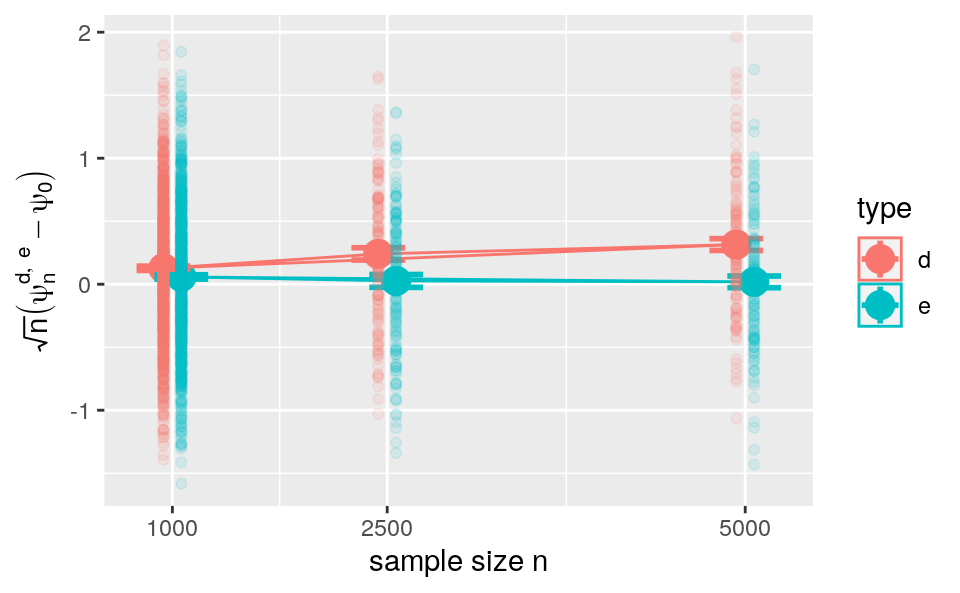
\includegraphics[width=0.7\linewidth]{img/estimating-Qbar-four-1} 

}

\caption{Evolution of root-\(n\) times bias versus sample size for two G-computation estimators of \(\psi_{0}\). The estimators respectively hinge on algorithms \(\Algo_{\Qbar,1}\) (d) and \(\Algo_{\Qbar,\text{kNN}}\) (e) to estimate \(\Qbar_{0}\). Big dots represent the average biases and vertical lines represent twice the standard error.}\label{fig:estimating-Qbar-four}
\end{figure}

On the one hand, root-\(n\) bias for \(\psi_{n}^{e}\) tends to decrease from
sample size 1000 to 5000 where it tends to be small in
average.\footnote{We use the expression ``tend to be'\,' because controlling for
  multiple testing makes it impossible to make a firm statement.} On the other
hand, root-\(n\) bias for \(\psi_{n}^{d}\) (red lines and points) is positive and
tends to increase from sample size 1000 to 2500 and from
2500 to 5000. Overall, root-\(n\) bias tends to be
larger for \(\psi_{n}^{d}\) than for \(\psi_{n}^{e}\).

In essence, we observe that the bias does not vanish faster than root-\(n\). For
\(\psi_{n}^{d}\), this is because \(\Algo_{\Qbar,1}\) is mis-specified and we
expect that the bias increases at rate root-\(n\). For \(\psi_{n}^{e}\), this is
because the estimator produced by the versatile \(\Algo_{\Qbar,\text{kNN}}\)
converges slowly to its limit. Can anything be done to amend \(\psi_{n}^{d}\)
and \(\psi_{n}^{e}\)?

\hypertarget{exo-plug-in-estimate}{%
\section{\texorpdfstring{⚙ \gear Investigating further the G-computation estimation strategy}{⚙ Investigating further the G-computation estimation strategy}}\label{exo-plug-in-estimate}}

\begin{enumerate}
\def\labelenumi{\arabic{enumi}.}
\item
  Implement the G-computation estimator based on well-specified working
  model. To do so, \emph{(i)} create a copy \texttt{working\_model\_Q\_two} of
  \texttt{working\_model\_Q\_one}, \emph{(ii)} replace its \texttt{family} entry in such a way that
  \(\Qbar_{0}\) falls in the corresponding working model, and \emph{(iii)} adapt the
  chunk of code where we computed \texttt{Qbar\_hat\_d} in Section
  \ref{Gcomp-construction}.
\item
  Evaluate the empirical properties of the estimator of problem 1.
\item
  Create a function to estimate the marginal law \(Q_{0,W}\) of \(W\) by maximum
  likelihood estimation based on a mis-specified model that assumes (wrongly)
  that \(W\) is drawn from a Gaussian law with unknown mean and variance.
\item
  ☡ \stixdanger{} Implement the G-computation estimator using either
  \texttt{working\_model\_Q\_one} or \texttt{working\_model\_Q\_two} and the estimator of
  \(Q_{0,W}\) of problem 3.
\end{enumerate}

\hypertarget{one-step}{%
\chapter{One-step correction}\label{one-step}}

\hypertarget{analysis-of-plug-in}{%
\section{\texorpdfstring{☡ \stixdanger{} General analysis of plug-in estimators}{☡  General analysis of plug-in estimators}}\label{analysis-of-plug-in}}

Recall that \(\Algo_{Q_{W}}\) is an algorithm designed for the estimation of
\(Q_{0,W}\) (see Section \ref{nuisance-QW}) and that we denote by \(Q_{n,W} \defq \Algo_{Q_{W}}(P_{n})\) the output of the algorithm trained on \(P_{n}\).
Likewise, \(\Algo_{\Gbar}\) and \(\Algo_{\Qbar}\) are two generic algorithms
designed for the estimation of \(\Gbar_{0}\) and of \(\Qbar_{0}\) (see Sections
\ref{nuisance-Gbar} and \ref{nuisance-Qbar}), \(\Gbar_{n} \defq \Algo_{\Gbar}(P_{n})\) and \(\Qbar_{n} \defq \Algo_{\Qbar}(P_{n})\) are their
outputs once trained on \(P_{n}\).

Let us now introduce \(\Phat_n\) a law in \(\calM\) such that the \(Q_{W}\), \(\Gbar\)
and \(\Qbar\) features of \(\Phat_n\) equal \(Q_{n,W}\), \(\Gbar_{n}\) and
\(\Qbar_{n}\), respectively. We say that any such law is \emph{compatible} with
\(Q_{n,W}\), \(\Gbar_n\) and \(\Qbar_n\).

Now, let us substitute \(\Phat_n\) for \(P\) in \eqref{eq:taylor-expansion}:

\begin{equation} 
\label{eq:hard-to-study}  \Psi(\Phat_n)  -  \Psi(P_0)   =  -  P_0  D^*(\Phat_n)  +
\Rem_{P_0}(\Phat_n) . 
\end{equation}

We show \protect\hyperlink{app-analysis-of-plug-in}{there} in Appendix
\ref{app-analysis-of-plug-in} that, under conditions on the
complexity/versatility of algorithms \(\Algo_{\Gbar}\) and \(\Algo_{\Qbar}\)
(often referred to as \emph{regularity conditions}) and assuming that their outputs
\(\Gbar_{n}\) and \(\Qbar_{n}\) both consistently estimate their targets
\(\Gbar_{0}\) and \(\Qbar_{0}\), it holds that

\begin{align} 
\Psi(\Phat_n) - \Psi(P_0) &= - P_{n} D^*(\Phat_n) +
 P_{n} D^*(P_0) + 
o_{P_0}(1/\sqrt{n}) \label{eq:pre-one-step} \\ 
\notag &= - P_{n} D^*(\Phat_n)+ \frac{1}{n} \sum_{i=1}^n D^*(P_0)(O_i)  + o_{P_0}(1/\sqrt{n}). 
\end{align}

In light of \eqref{eq:asymptotic-lin}, \(\Psi(\Phat_{n})\) would be
asymptotically linear with influence curve \(\IC=D^{*}(P_{0})\) in the absence of
the random term \(-P_{n} D^*(\Phat_n)\). Unfortunately, it turns out that this
term can degrade dramatically the behavior of the plug-in estimator
\(\Psi(\Phat_{n})\).

\hypertarget{huber-one-step}{%
\section{One-step correction}\label{huber-one-step}}

Luckily, \emph{a very simple workaround} allows to circumvent the problem. Proposed
in \citep{LeCam69} (see also \citep{Pfanzagl82} and \citep{vdV98}), the workaround merely
consists in adding the random term to the initial estimator, that is, in
estimating \(\Psi(P_0)\) not with \(\Psi(\Phat_n)\) but instead with
\begin{equation}
\psinos  \defq  \Psi(\Phat_n)  +  P_{n} D^*(\Phat_n)  =  \Psi(\Phat_n)  +
\frac{1}{n} \sum_{i=1}^{n} D^*(\Phat_n)(O_{i}). \label{eq:def-one-step}
\end{equation}

Obviously, in light of \eqref{eq:pre-one-step}, \(\psinos\) is asymptotically
linear with influence curve \(\IC=D^{*}(P_{0})\). Thus, by the central limit
theorem, \(\sqrt{n} (\psinos - \Psi(P_0))\) converges in law to a centered
Gaussian distribution with variance
\begin{equation}
  \Var_{P_0}(D^{*}(P_{0})(O)) = \Exp_{P_0}(D^{*}(P_{0})(O)).
\end{equation}

The detailed general analysis of plug-in estimators
developed \protect\hyperlink{app-analysis-of-plug-in}{there} in Appendix
\ref{app-analysis-of-plug-in} also revealed that the above asymptotic
variance is consistently estimated with \begin{equation}    P_{n}
D^{*}(\Phat_{n})^{2}  =  \frac{1}{n}  \sum_{i=1}^{n}  D^*(\Phat_n)^{2}(O_{i}).
\end{equation} Therefore, by the central limit theorem and Slutsky's lemma
(see the argument \protect\hyperlink{clt}{there} in Appendix \ref{clt}), \begin{equation*}
\left[\psinos           \pm          \Phi^{-1}(1-\alpha)           \frac{P_{n}
D^{*}(\Phat_{n})^{2}}{\sqrt{n}}\right]   \end{equation*} is a confidence
interval for \(\Psi(P_0)\) with asymptotic level \((1-2\alpha)\).

\hypertarget{empirical-inves-one-step}{%
\section{Empirical investigation}\label{empirical-inves-one-step}}

In light of \eqref{eq:def-one-step} if the estimator equals \(\Psi(\Phat_{n})\),
then performing a one-step correction essentially boils down to computing two
quantities, \(-P_{n} D^{*}(\Phat_{n})\) (the bias term) and \(P_{n} D^{*}(\Phat_{n})^{2}\) (an estimator of the asymptotic variance of
\(\psinos\)). The \texttt{tlrider} package makes the operation very easy thanks to the
function \texttt{apply\_one\_step\_correction}.

Let us illustrate its use by updating the G-computation estimator built on the
\(n=1000\) first observations in \texttt{obs} by relying on \(\Algo_{\Qbar,\text{kNN}}\),
that is, on the algorithm for the estimation of \(\Qbar_{0}\) as it is
implemented in \texttt{estimate\_Qbar} with its argument \texttt{algorithm} set to the
built-in \texttt{kknn\_algo} (see Section \ref{Qbar-knn-algo}). The algorithm has
been trained earlier on this data set and produced the object \texttt{Qbar\_hat\_kknn}.
The following chunk of code re-computes the corresponding G-computation
estimator, using again the estimator \texttt{QW\_hat} of the marginal law of \(W\) under
\(P_{0}\) (see Section \ref{nuisance-QW}), then applied the one-step correction:

\begin{Shaded}
\begin{Highlighting}[]
\NormalTok{(psin\_kknn }\OtherTok{\textless{}{-}} \FunctionTok{compute\_gcomp}\NormalTok{(QW\_hat, }\FunctionTok{wrapper}\NormalTok{(Qbar\_hat\_kknn, }\ConstantTok{FALSE}\NormalTok{), }\FloatTok{1e3}\NormalTok{))}
\CommentTok{\#\textgreater{} \# A tibble: 1 x 2}
\CommentTok{\#\textgreater{}   psi\_n   sig\_n}
\CommentTok{\#\textgreater{}   \textless{}dbl\textgreater{}   \textless{}dbl\textgreater{}}
\CommentTok{\#\textgreater{} 1 0.101 0.00306}
\NormalTok{(psin\_kknn\_os }\OtherTok{\textless{}{-}} \FunctionTok{apply\_one\_step\_correction}\NormalTok{(}\FunctionTok{head}\NormalTok{(obs, }\FloatTok{1e3}\NormalTok{),}
                                           \FunctionTok{wrapper}\NormalTok{(Gbar\_hat, }\ConstantTok{FALSE}\NormalTok{),}
                                           \FunctionTok{wrapper}\NormalTok{(Qbar\_hat\_kknn, }\ConstantTok{FALSE}\NormalTok{),}
\NormalTok{                                           psin\_kknn}\SpecialCharTok{$}\NormalTok{psi\_n)) }
\CommentTok{\#\textgreater{} \# A tibble: 1 x 3}
\CommentTok{\#\textgreater{}    psi\_n  sig\_n    crit\_n}
\CommentTok{\#\textgreater{}    \textless{}dbl\textgreater{}  \textless{}dbl\textgreater{}     \textless{}dbl\textgreater{}}
\CommentTok{\#\textgreater{} 1 0.0999 0.0171 {-}0.000633}
\end{Highlighting}
\end{Shaded}

In the call to \texttt{apply\_one\_step\_correction} we provide \emph{(i)} the data set at
hand (first line), \emph{(ii)} the estimator \texttt{Gbar\_hat} of \(\Gbar_{0}\) that we
built earlier by using algorithm \(\Algo_{\Gbar,1}\) (second line; see Section
\ref{algo-Gbar-one}), \emph{(iii)} the estimator \texttt{Qbar\_hat\_kknn} of \(\Qbar_{0}\)
and the G-computation estimator \texttt{psin\_kknn} that resulted from it (third and
fourth lines).

To assess what is the impact of the one-step correction, let us apply the
one-step correction to the estimators that we built in Section
\ref{empirical-inves-Gcomp}. The object \texttt{learned\_features\_fixed\_sample\_size}
already contains the estimated features of \(P_{0}\) that are needed to perform
the one-step correction to the estimators \(\psi_{n}^{d}\) and \(\psi_{n}^{e}\),
namely, thus we merely have to call the function \texttt{apply\_one\_step\_correction}.



\begin{Shaded}
\begin{Highlighting}[]
\NormalTok{psi\_hat\_de\_one\_step }\OtherTok{\textless{}{-}}\NormalTok{ learned\_features\_fixed\_sample\_size }\SpecialCharTok{\%\textgreater{}\%}
  \FunctionTok{mutate}\NormalTok{(}\AttributeTok{os\_est\_d =}
           \FunctionTok{pmap}\NormalTok{(}\FunctionTok{list}\NormalTok{(obs, Gbar\_hat, Qbar\_hat\_d, est\_d),}
                \SpecialCharTok{\textasciitilde{}} \FunctionTok{apply\_one\_step\_correction}\NormalTok{(}\FunctionTok{as.matrix}\NormalTok{(..}\DecValTok{1}\NormalTok{),}
                                 \FunctionTok{wrapper}\NormalTok{(..}\DecValTok{2}\NormalTok{, }\ConstantTok{FALSE}\NormalTok{),}
                                 \FunctionTok{wrapper}\NormalTok{(..}\DecValTok{3}\NormalTok{, }\ConstantTok{FALSE}\NormalTok{),}
\NormalTok{                                 ..}\DecValTok{4}\SpecialCharTok{$}\NormalTok{psi\_n)),}
         \AttributeTok{os\_est\_e =}
           \FunctionTok{pmap}\NormalTok{(}\FunctionTok{list}\NormalTok{(obs, Gbar\_hat, Qbar\_hat\_e, est\_e),}
                \SpecialCharTok{\textasciitilde{}} \FunctionTok{apply\_one\_step\_correction}\NormalTok{(}\FunctionTok{as.matrix}\NormalTok{(..}\DecValTok{1}\NormalTok{),}
                                 \FunctionTok{wrapper}\NormalTok{(..}\DecValTok{2}\NormalTok{, }\ConstantTok{FALSE}\NormalTok{),}
                                 \FunctionTok{wrapper}\NormalTok{(..}\DecValTok{3}\NormalTok{, }\ConstantTok{FALSE}\NormalTok{),}
\NormalTok{                                 ..}\DecValTok{4}\SpecialCharTok{$}\NormalTok{psi\_n))) }\SpecialCharTok{\%\textgreater{}\%}
  \FunctionTok{select}\NormalTok{(os\_est\_d, os\_est\_e) }\SpecialCharTok{\%\textgreater{}\%}
  \FunctionTok{pivot\_longer}\NormalTok{(}\FunctionTok{c}\NormalTok{(}\StringTok{\textasciigrave{}}\AttributeTok{os\_est\_d}\StringTok{\textasciigrave{}}\NormalTok{, }\StringTok{\textasciigrave{}}\AttributeTok{os\_est\_e}\StringTok{\textasciigrave{}}\NormalTok{),}
               \AttributeTok{names\_to =} \StringTok{"type"}\NormalTok{, }\AttributeTok{values\_to =} \StringTok{"estimates"}\NormalTok{) }\SpecialCharTok{\%\textgreater{}\%}
  \FunctionTok{extract}\NormalTok{(type, }\StringTok{"type"}\NormalTok{, }\StringTok{"\_([de])$"}\NormalTok{) }\SpecialCharTok{\%\textgreater{}\%}
  \FunctionTok{mutate}\NormalTok{(}\AttributeTok{type =} \FunctionTok{paste0}\NormalTok{(type, }\StringTok{"\_one\_step"}\NormalTok{)) }\SpecialCharTok{\%\textgreater{}\%}
  \FunctionTok{unnest}\NormalTok{(estimates) }\SpecialCharTok{\%\textgreater{}\%}
  \FunctionTok{group\_by}\NormalTok{(type) }\SpecialCharTok{\%\textgreater{}\%}
  \FunctionTok{mutate}\NormalTok{(}\AttributeTok{sig\_alt =} \FunctionTok{sd}\NormalTok{(psi\_n)) }\SpecialCharTok{\%\textgreater{}\%}
  \FunctionTok{mutate}\NormalTok{(}\AttributeTok{clt\_ =}\NormalTok{ (psi\_n }\SpecialCharTok{{-}}\NormalTok{ psi\_zero) }\SpecialCharTok{/}\NormalTok{ sig\_n,}
         \AttributeTok{clt\_alt =}\NormalTok{ (psi\_n }\SpecialCharTok{{-}}\NormalTok{ psi\_zero) }\SpecialCharTok{/}\NormalTok{ sig\_alt) }\SpecialCharTok{\%\textgreater{}\%}
  \FunctionTok{pivot\_longer}\NormalTok{(}\FunctionTok{c}\NormalTok{(}\StringTok{\textasciigrave{}}\AttributeTok{clt\_}\StringTok{\textasciigrave{}}\NormalTok{, }\StringTok{\textasciigrave{}}\AttributeTok{clt\_alt}\StringTok{\textasciigrave{}}\NormalTok{),}
               \AttributeTok{names\_to =} \StringTok{"key"}\NormalTok{, }\AttributeTok{values\_to =} \StringTok{"clt"}\NormalTok{) }\SpecialCharTok{\%\textgreater{}\%}
  \FunctionTok{extract}\NormalTok{(key, }\StringTok{"key"}\NormalTok{, }\StringTok{"\_(.*)$"}\NormalTok{) }\SpecialCharTok{\%\textgreater{}\%}
  \FunctionTok{mutate}\NormalTok{(}\AttributeTok{key =} \FunctionTok{ifelse}\NormalTok{(key }\SpecialCharTok{==} \StringTok{""}\NormalTok{, }\ConstantTok{TRUE}\NormalTok{, }\ConstantTok{FALSE}\NormalTok{)) }\SpecialCharTok{\%\textgreater{}\%}
  \FunctionTok{rename}\NormalTok{(}\StringTok{"auto\_renormalization"} \OtherTok{=}\NormalTok{ key)}
  
\NormalTok{(bias\_de\_one\_step }\OtherTok{\textless{}{-}}\NormalTok{ psi\_hat\_de\_one\_step }\SpecialCharTok{\%\textgreater{}\%}
   \FunctionTok{group\_by}\NormalTok{(type, auto\_renormalization) }\SpecialCharTok{\%\textgreater{}\%}
   \FunctionTok{summarize}\NormalTok{(}\AttributeTok{bias =} \FunctionTok{mean}\NormalTok{(clt)) }\SpecialCharTok{\%\textgreater{}\%}\NormalTok{ ungroup)}
\CommentTok{\#\textgreater{} \# A tibble: 4 x 3}
\CommentTok{\#\textgreater{}   type       auto\_renormalization     bias}
\CommentTok{\#\textgreater{}   \textless{}chr\textgreater{}      \textless{}lgl\textgreater{}                   \textless{}dbl\textgreater{}}
\CommentTok{\#\textgreater{} 1 d\_one\_step FALSE                {-}0.0142 }
\CommentTok{\#\textgreater{} 2 d\_one\_step TRUE                 {-}0.0307 }
\CommentTok{\#\textgreater{} 3 e\_one\_step FALSE                 0.0126 }
\CommentTok{\#\textgreater{} 4 e\_one\_step TRUE                 {-}0.00460}

\NormalTok{fig }\OtherTok{\textless{}{-}} \FunctionTok{ggplot}\NormalTok{() }\SpecialCharTok{+}
  \FunctionTok{geom\_line}\NormalTok{(}\FunctionTok{aes}\NormalTok{(}\AttributeTok{x =}\NormalTok{ x, }\AttributeTok{y =}\NormalTok{ y), }
            \AttributeTok{data =} \FunctionTok{tibble}\NormalTok{(}\AttributeTok{x =} \FunctionTok{seq}\NormalTok{(}\SpecialCharTok{{-}}\DecValTok{4}\NormalTok{, }\DecValTok{4}\NormalTok{, }\AttributeTok{length.out =} \FloatTok{1e3}\NormalTok{),}
                          \AttributeTok{y =} \FunctionTok{dnorm}\NormalTok{(x)),}
            \AttributeTok{linetype =} \DecValTok{1}\NormalTok{, }\AttributeTok{alpha =} \FloatTok{0.5}\NormalTok{) }\SpecialCharTok{+}
  \FunctionTok{geom\_density}\NormalTok{(}\FunctionTok{aes}\NormalTok{(clt, }\AttributeTok{fill =}\NormalTok{ type, }\AttributeTok{colour =}\NormalTok{ type),}
\NormalTok{               psi\_hat\_de\_one\_step, }\AttributeTok{alpha =} \FloatTok{0.1}\NormalTok{) }\SpecialCharTok{+}
  \FunctionTok{geom\_vline}\NormalTok{(}\FunctionTok{aes}\NormalTok{(}\AttributeTok{xintercept =}\NormalTok{ bias, }\AttributeTok{colour =}\NormalTok{ type),}
\NormalTok{             bias\_de\_one\_step, }\AttributeTok{size =} \FloatTok{1.5}\NormalTok{, }\AttributeTok{alpha =} \FloatTok{0.5}\NormalTok{) }\SpecialCharTok{+}
  \FunctionTok{facet\_wrap}\NormalTok{(}\SpecialCharTok{\textasciitilde{}}\NormalTok{ auto\_renormalization,}
             \AttributeTok{labeller =}
               \FunctionTok{as\_labeller}\NormalTok{(}\FunctionTok{c}\NormalTok{(}\StringTok{\textasciigrave{}}\AttributeTok{TRUE}\StringTok{\textasciigrave{}} \OtherTok{=} \StringTok{"auto{-}renormalization: TRUE"}\NormalTok{,}
                             \StringTok{\textasciigrave{}}\AttributeTok{FALSE}\StringTok{\textasciigrave{}} \OtherTok{=} \StringTok{"auto{-}renormalization: FALSE"}\NormalTok{)),}
             \AttributeTok{scales =} \StringTok{"free"}\NormalTok{)}
  
\NormalTok{fig }\SpecialCharTok{+}
  \FunctionTok{labs}\NormalTok{(}\AttributeTok{y =} \StringTok{""}\NormalTok{,}
       \AttributeTok{x =} \FunctionTok{bquote}\NormalTok{(}\FunctionTok{paste}\NormalTok{(}\FunctionTok{sqrt}\NormalTok{(n}\SpecialCharTok{/}\NormalTok{v[n]}\SpecialCharTok{\^{}}\NormalTok{\{}\FunctionTok{list}\NormalTok{(d, e, os)\})}\SpecialCharTok{*}
\NormalTok{                        (psi[n]}\SpecialCharTok{\^{}}\NormalTok{\{}\FunctionTok{list}\NormalTok{(d, e, os)\} }\SpecialCharTok{{-}}\NormalTok{ psi[}\DecValTok{0}\NormalTok{]))))}
\end{Highlighting}
\end{Shaded}

\begin{figure}

{\centering 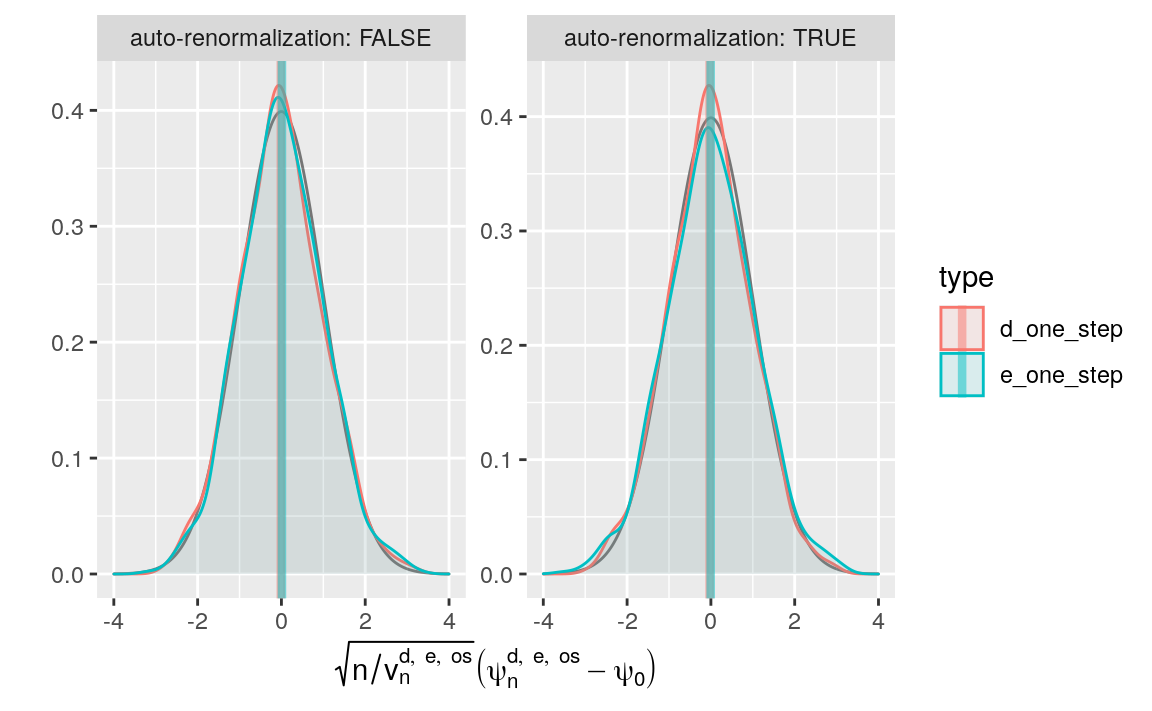
\includegraphics[width=0.7\linewidth]{img/one-step-one-1} 

}

\caption{Kernel density estimators of the law of two one-step-G-computation estimators of \(\psi_{0}\) (recentered with respect to \(\psi_{0}\), and renormalized). The estimators respectively hinge on algorithms \(\Algo_{\Qbar,1}\) (d) and \(\Algo_{\Qbar,\text{kNN}}\) (e) to estimate \(\Qbar_{0}\), and on one-step correction. Two renormalization schemes are considered, either based on an estimator of the asymptotic variance (left) or on the empirical variance computed across the 1000 independent replications of the estimators (right). We emphasize that the \(x\)-axis ranges differ between the left and right plots.}\label{fig:one-step-one}
\end{figure}

It seems that the one-step correction performs quite well (in particular,
compare \texttt{bias\_de} with \texttt{bias\_de\_one\_step}):

\begin{Shaded}
\begin{Highlighting}[]
\FunctionTok{bind\_rows}\NormalTok{(bias\_de, bias\_de\_one\_step) }\SpecialCharTok{\%\textgreater{}\%}
  \FunctionTok{filter}\NormalTok{(}\SpecialCharTok{!}\NormalTok{auto\_renormalization) }\SpecialCharTok{\%\textgreater{}\%}
  \FunctionTok{arrange}\NormalTok{(type)}
\CommentTok{\#\textgreater{} \# A tibble: 4 x 3}
\CommentTok{\#\textgreater{}   type       auto\_renormalization    bias}
\CommentTok{\#\textgreater{}   \textless{}chr\textgreater{}      \textless{}lgl\textgreater{}                  \textless{}dbl\textgreater{}}
\CommentTok{\#\textgreater{} 1 d          FALSE                 0.234 }
\CommentTok{\#\textgreater{} 2 d\_one\_step FALSE                {-}0.0142}
\CommentTok{\#\textgreater{} 3 e          FALSE                 0.107 }
\CommentTok{\#\textgreater{} 4 e\_one\_step FALSE                 0.0126}
\end{Highlighting}
\end{Shaded}

What about the estimation of the asymptotic variance, and of the mean squared-error of the estimators?

\begin{Shaded}
\begin{Highlighting}[]
\NormalTok{psi\_hat\_de }\SpecialCharTok{\%\textgreater{}\%}
  \FunctionTok{full\_join}\NormalTok{(psi\_hat\_de\_one\_step) }\SpecialCharTok{\%\textgreater{}\%}
  \FunctionTok{filter}\NormalTok{(auto\_renormalization) }\SpecialCharTok{\%\textgreater{}\%} 
  \FunctionTok{group\_by}\NormalTok{(type) }\SpecialCharTok{\%\textgreater{}\%}
  \FunctionTok{summarize}\NormalTok{(}\AttributeTok{sd =} \FunctionTok{mean}\NormalTok{(sig\_n),}
            \AttributeTok{se =} \FunctionTok{sd}\NormalTok{(psi\_n),}
            \AttributeTok{mse =} \FunctionTok{mean}\NormalTok{((psi\_n }\SpecialCharTok{{-}}\NormalTok{ psi\_zero)}\SpecialCharTok{\^{}}\DecValTok{2}\NormalTok{) }\SpecialCharTok{*} \FunctionTok{n}\NormalTok{()) }\SpecialCharTok{\%\textgreater{}\%}
  \FunctionTok{arrange}\NormalTok{(type)}
\CommentTok{\#\textgreater{} \# A tibble: 4 x 4}
\CommentTok{\#\textgreater{}   type            sd     se   mse}
\CommentTok{\#\textgreater{}   \textless{}chr\textgreater{}        \textless{}dbl\textgreater{}  \textless{}dbl\textgreater{} \textless{}dbl\textgreater{}}
\CommentTok{\#\textgreater{} 1 d          0.00206 0.0171 0.309}
\CommentTok{\#\textgreater{} 2 d\_one\_step 0.0173  0.0171 0.291}
\CommentTok{\#\textgreater{} 3 e          0.00288 0.0172 0.298}
\CommentTok{\#\textgreater{} 4 e\_one\_step 0.0166  0.0175 0.305}
\end{Highlighting}
\end{Shaded}

The \texttt{sd} (\emph{estimator} of the asymptotic standard deviation) and \texttt{se}
(\emph{empirical} standard deviation) entries are similar. This indicates that the
inference of the asymptotic variance of the one-step estimators based on the
influence curve is rather accurate for both the \texttt{d}- and \texttt{e}-variants that we
implemented. As for the mean square error, it is made respectively slightly
smaller or bigger or by the one-step update for type \texttt{d} and \texttt{e}, the
\texttt{d\_one\_step} estimator exhibiting the smallest mean square error.

\hypertarget{exo-one-step}{%
\section{\texorpdfstring{⚙ \gear Investigating further the one-step correction methodology}{⚙ Investigating further the one-step correction methodology}}\label{exo-one-step}}

\begin{enumerate}
\def\labelenumi{\arabic{enumi}.}
\item
  Use \texttt{estimate\_Gbar} to create an oracle algorithm \(\Algora_{\Gbar,s}\) for
  the estimation of \(\Gbar_{0}\) that, for any \(s > 0\), estimates
  \(\Gbar_{0}(w)\) with \begin{equation*}    \Gbar_{n}(w)   \defq
  \Algora_{\Gbar,s}                     (P_{n})(w)                    \defq
  \expit\left(\logit\left(\Gbar_{0}(w)\right) +  s Z\right) \end{equation*}
  where \(Z\) is a standard normal random variable.\footnote{Note that the algorithm
    does not really to be trained.} What would happen if one chose \(s=0\) in the
  above definition? What happens when \(s\) converges to 0? Explain why the algorithm
  is said to be an \emph{oracle algorithm}.
\item
  Use \texttt{estimate\_Qbar} to create an oracle algorithm \(\Algora_{\Qbar,s}\) for
  the estimation of \(\Qbar_{0}\) that, for any \(s > 0\), estimates
  \(\Qbar_{0}(a,w)\) with \begin{equation*}    \Qbar_{n}(a,w)   \defq
  \Algora_{\Gbar,s}                     (P_{n})(a,w)                    \defq 
  \expit\left(\logit\left(\Qbar_{0}(a,w)\right) +  s Z\right) \end{equation*}
  where \(Z\) is a standard normal random variable. The comments made about
  \(\Algora_{\Gbar,s}\) in the above problem also apply to \(\Algora_{\Qbar,s}\).
\item
  Reproduce the simulation study developed in Sections \ref{empirical-inves-Gcomp}
  and \ref{empirical-inves-one-step} with the oracle algorithms \(\Algora_{\Gbar,s}\)
  and \(\Algora_{\Qbar,s'}\) substituted for used in these sections. Change the values
  of \(s,s' > 0\) and compare how well the estimating procedure performs depending on the product \(ss'\).
  What do you observe? We invite you to refer to Section \ref{app-analysis-of-plug-in-main}.
\end{enumerate}

\hypertarget{TMLE}{%
\chapter{Targeted minimum loss-based estimation}\label{TMLE}}

\hypertarget{TMLE-motivations}{%
\section{Motivations}\label{TMLE-motivations}}

\hypertarget{falling-outside-the-parameter-space}{%
\subsection{Falling outside the parameter space}\label{falling-outside-the-parameter-space}}

Section \ref{one-step} introduced the one-step corrected estimator \(\psinos\)
of \(\psi_0\). It is obtained by adding a correction term to an initial plug-in
estimator \(\Psi(\Phat_{n})\), resulting in an estimator that is asymptotically
linear with influence curve \(\IC = D^{*}(P_{0})\) under mild conditions (see
Section \ref{huber-one-step} and the detailed
proof \protect\hyperlink{app-analysis-of-plug-in}{there} in Appendix
\ref{app-analysis-of-plug-in}).

Unfortunately, the one-step estimator lacks a desirable feature of a plug-in
estimator: plug-in estimators always lie in the parameter space whereas a
one-step estimator does not necessarily do so. For example, it must also be
true that \(\psi_0 = \Psi(P_{0}) \in [-1,1]\) yet it may be the case that
\(\psinos \not\in[-1,1]\).

It is typically easy to shape an algorithm \(\Algo_{\Qbar}\) for the estimation
of \(\Qbar_0\) to output estimators \(\Qbar_n\) that, like \(\Qbar_{0}\), take their
values in \([0,1]\). The plug-in estimator \(\psi_{n}\) \eqref{eq:Gcomp-estimator}
based on such a \(\Qbar_{n}\) necessarily satisfies \(\psi_{n} \in [-1,1]\).
However, the one-step estimator derived from \(\psi_{n}\) may fall outside of
the interval if the correction term \(P_{n} D^{*} (\Phat_{n})\) is large.

\hypertarget{eic-equation}{%
\subsection{The influence curve equation}\label{eic-equation}}

Upon closer examination of the influence curve \(D^*(\Phat_{n})\), we see that
this may occur more frequently when \(\ell \Gbar_n(A_i,W_i)\) is close to zero
for at least some \(1 \leq i\leq n\). In words, this may happen if there are
observations in our data set that we observed under actions \(A_i\) that were
estimated to be unlikely given their respective contexts \(W_i\). In such
cases, \(D^*(\Phat_n)(O_i)\), and consequently the one-step correction term, may
be large and cause the one-step estimate to fall outside \([-1,1]\).

Another way to understand this behavior is to recognize the one-step estimator
as an initial plug-in estimator that is corrected \emph{in the parameter space of}
\(\psi_0\). One of the pillars of targeted learning is to perform, instead, a
correction \emph{in the parameter space of} \(\Qbar_0\).

In particular, consider a law \(P_{n}^{*}\) estimating \(P_{0}\) that is
compatible with the estimators \(\Qbar_n^*\), \(\Gbar_n\), and \(Q_{n,W}\), but
moreover is such that
\begin{equation} 
P_n  D^*(P_{n}^*)  = 0 \label{eq:solve}
\end{equation}
or, at the very least,
\begin{equation} 
P_n D^*(P_{n}^*) = o_{P_0}(1/\sqrt{n}). \label{eq:solve-approx} 
\end{equation}
Achieving \eqref{eq:solve} is called \emph{solving the efficient influence curve
equation}. Likewise, achieving \eqref{eq:solve-approx} is called
\emph{approximately solving the influence curve equation}.

If such estimators can be generated indeed, then the plug-in estimator
\begin{equation*}     \psi_n^*    \defq     \Psi(P_{n}^{*})    =     \int
\left(\Qbar_n^*(1,w)  - \Qbar_n^*(0,w)\right)  dQ_{n,W}(w) \end{equation*} is
asymptotically linear with influence curve \(\IC = D^{*}(P_{0})\), under mild
conditions. Moreover, by virtue of its plug-in construction, it has the
additional property that in finite-samples \(\psi_n^*\) will always obey bounds
on the parameter space.

\hypertarget{basic-fact}{%
\subsection{A basic fact on the influence curve equation}\label{basic-fact}}

Our strategy for constructing such a plug-in estimate begins by generating an
initial estimator \(\Qbar_n\) of \(\Qbar_0\) based on an algorithm \(\Algo_{\Qbar}\)
and an estimator \(\Gbar_n\) of \(\Gbar_0\) based on an algorithm \(\Algo_{\Gbar}\).
These initial estimators should strive to be as close as possible to their
respective targets. We use the empirical distribution \(Q_{n,W}\) as an
estimator of \(Q_{0,W}\).

Now, recall the definition of \(D_{1}^{*}\) \eqref{eq:eif} and note that for
\emph{any} estimator \(\Qbar_n^*\) of \(\Qbar_0\) and a law \(P_n^{*}\) that is
compatible with \(\Qbar_n^*\) and \(Q_{n,W}\), \begin{equation*}  P_{n}  D_{1}
(P_{n}^{*}) = 0.
\end{equation*}
The proof can be found \protect\hyperlink{basic-eic-eq}{there} in Appendix \ref{basic-eic-eq}.

In words, this shows that so long as we use the empirical distribution
\(Q_{n,W}\) to estimate \(Q_{0,W}\), by its very construction achieving
\eqref{eq:solve} or \eqref{eq:solve-approx} is equivalent to solving
\begin{equation} 
P_n  D_{2}^*(P_{n}^*)  = 0 \label{eq:solve-alt}
\end{equation}
or
\begin{equation} 
P_n D_{2}^*(P_{n}^*) = o_{P_0}(1/\sqrt{n}). \label{eq:solve-approx-alt} 
\end{equation}

It thus remains to devise a strategy for ensuring that \(P_n D_2^*(P_n^*) = 0\) or \(o_{P_0}(1/\sqrt{n})\).

\hypertarget{targeted-fluctuation-TMLE}{%
\section{Targeted fluctuation}\label{targeted-fluctuation-TMLE}}

Our approach to satisfying \eqref{eq:solve-alt}\footnote{or \eqref{eq:solve-approx-alt}.}
hinges on revising our initial estimator \(\Qbar_n\) of \(\Qbar_0\). We propose a
method for building an estimator of \(\Qbar_0\) that is ``near to'' \(\Qbar_n\), but
is such that for any law \(P_n^*\) that is compatible with this revised
estimator, \(P_n D^*(P_n^*) = 0\).\footnote{or \(P_n D^*(P_n^*) = o_{P_0}(1/\sqrt{n})\).}
Because \(\Qbar_n\) is our best (initial) estimator of \(\Qbar_0\), the new
estimator that we shall build should be \emph{at least as good} an estimator of
\(\Qbar_0\) as \(\Qbar_n\). So first, we must propose a way to move between
regression functions, and then we must propose a way to move to a new
regression function that fits the data at least as well as \(\Qbar_n\).

Instead of writing ``propos{[}ing{]} a way to move between regression functions'' we
may also have written ``proposing a way to \emph{fluctuate} a regression function'',
thus suggesting very opportunely that the notion of fluctuation as discussed
in Section \ref{smooth-second-pass} may prove instrumental to achieve the
former objective.

\hypertarget{fluctuating-indirectly}{%
\subsection{\texorpdfstring{☡ \stixdanger{} Fluctuating indirectly}{☡  Fluctuating indirectly}}\label{fluctuating-indirectly}}

Let us resume the discussion where we left it at the end of Section
\ref{smooth-second-pass-fluctuations}. It is easy to show that the
fluctuation \(\{P_{h} : h \in H\}\) of \(P\) in direction of \(s\) in \(\calM\)
induces a fluctuation \(\{\Qbar_{h} : h \in H\}\) of \(\Qbar = \left.Q_{h}\right|_{h=0}\) in the space \(\calQ \defq \{\Qbar : P \in \calM\}\) of regression functions induced by model \(\calM\). Specifically we
show \protect\hyperlink{fluct-reg}{there} in Appendix \ref{fluct-reg} that, for every \(h \in H\), the conditional mean \(\Qbar_{h}(A,W)\) of \(Y\) given \((A,W)\) under \(P_{h}\)
is given by \begin{equation*}\Qbar_{h}(A,W)  \defq \frac{\Qbar(A,W)  + h
\Exp_{P}(Ys(O) | A,W)}{1 + h \Exp_{P}(s(O)|A,W)}.\end{equation*}

We note that if \(s(O)\) depends on \(O\) only through \((A,W)\) then, abusing
notation and writing \(s(A,W)\) for \(s(O)\),
\begin{align}
\Qbar_{h}(A,W)  &=  \frac{\Qbar(A,W)  +  h  \Exp_{P}(Ys(A,W)  |  A,W)}{1  +  h
\Exp_{P}(s(A,W)|A,W)}\notag\\&=\frac{\Qbar(A,W)  + h  s(A,W)\Qbar(A,W)}{1 +  h
s(A,W)}\notag\\&=\Qbar(A,W).\label{eq:Qbarh}
\end{align}
In words, \(\Qbar\) is not fluctuated at all, that is, the laws \(P_{h}\) that are
elements of the fluctuation share the same conditional mean of \(Y\) given
\((A,W)\).\footnote{In fact, more generally, the conditional \emph{law} of \(Y\) given \((A,W)\)
  is not fluctuated. See the corresponding problem in Section \ref{exo-fluct}.}

However we find it easier in the present context, notably from a computational
perspective, to fluctuate \(\Qbar_{n}\) \emph{directly} in \(\calQ\), as opposed to
\emph{indirectly} through a fluctuation defined in \(\calM\) of a law compatible with
\(\Qbar_{n}\). The next section introduces such a direct fluctuation.

\hypertarget{fluct-direct}{%
\subsection{Fluctuating directly}\label{fluct-direct}}

Set arbitrarily \(\Qbar \in \calQ\). The (direct) fluctuation of \(\Qbar\) that we
propose to consider depends on a user-supplied \(\Gbar\). For any \(\Gbar\) such
that \(0 < \ell\Gbar(A,W) < 1\), \(P_{0}\)-almost surely, the \(\Gbar\)-specific
fluctuation model for \(\Qbar\) is
\begin{equation} 
\calQ(\Qbar,\Gbar)\defq      \left\{(w,a)       \mapsto      \Qbar_{h}(a,w)      \defq
\expit\left(\logit\left(\Qbar(a,w)\right) +  h \frac{2a -  1}{\ell \Gbar(a,w)}
\right) : t \in \bbR\right\} \subset \calQ. \label{eq:Q-fluct} 
\end{equation}

Fluctuation \(\calQ(\Qbar,\Gbar)\) is a one-dimensional parametric model
(indexed by the real-valued parameter \(h\)) that goes through \(\Qbar\) (at
\(h=0\)). For each \(h \in \bbR\), \(\Qbar_{h} \in \calQ\) is the conditional mean
of \(Y\) given \((A,W)\) under infinitely many laws \(P \in \calM\).

The following chunk of code represents three elements of the fluctuations
\(\calQ(\Qbar_{0}, \Gbar_{0})\) and \(\calQ(\Qbar_{n,\text{trees}}, \Gbar_{0})\),
where \(\Qbar_{n,\text{trees}}\) is an estimator of \(\Qbar_{0}\) derived by the
boosted trees algorithm (see Section \ref{boosted-trees}).



\begin{Shaded}
\begin{Highlighting}[]
\NormalTok{Qbar\_hminus }\OtherTok{\textless{}{-}} \FunctionTok{fluctuate}\NormalTok{(Qbar, Gbar, }\AttributeTok{h =} \SpecialCharTok{{-}}\DecValTok{1}\NormalTok{)}
\NormalTok{Qbar\_hplus }\OtherTok{\textless{}{-}} \FunctionTok{fluctuate}\NormalTok{(Qbar, Gbar, }\AttributeTok{h =} \SpecialCharTok{+}\DecValTok{1}\NormalTok{)}

\NormalTok{Qbar\_trees }\OtherTok{\textless{}{-}} \FunctionTok{wrapper}\NormalTok{(Qbar\_hat\_trees, }\ConstantTok{FALSE}\NormalTok{)}
\NormalTok{Qbar\_trees\_hminus }\OtherTok{\textless{}{-}} \FunctionTok{fluctuate}\NormalTok{(Qbar\_trees, Gbar, }\AttributeTok{h =} \SpecialCharTok{{-}}\DecValTok{1}\NormalTok{)}
\NormalTok{Qbar\_trees\_hplus }\OtherTok{\textless{}{-}} \FunctionTok{fluctuate}\NormalTok{(Qbar\_trees, Gbar, }\AttributeTok{h =} \SpecialCharTok{+}\DecValTok{1}\NormalTok{)}

\FunctionTok{tibble}\NormalTok{(}\AttributeTok{w =} \FunctionTok{seq}\NormalTok{(}\DecValTok{0}\NormalTok{, }\DecValTok{1}\NormalTok{, }\AttributeTok{length.out =} \FloatTok{1e3}\NormalTok{)) }\SpecialCharTok{\%\textgreater{}\%}
  \FunctionTok{mutate}\NormalTok{(}\AttributeTok{truth\_0\_1 =} \FunctionTok{Qbar}\NormalTok{(}\FunctionTok{cbind}\NormalTok{(}\AttributeTok{A =} \DecValTok{1}\NormalTok{, }\AttributeTok{W =}\NormalTok{ w)),}
         \AttributeTok{truth\_0\_0 =} \FunctionTok{Qbar}\NormalTok{(}\FunctionTok{cbind}\NormalTok{(}\AttributeTok{A =} \DecValTok{0}\NormalTok{, }\AttributeTok{W =}\NormalTok{ w)),}
         \AttributeTok{trees\_0\_1 =} \FunctionTok{Qbar\_trees}\NormalTok{(}\FunctionTok{cbind}\NormalTok{(}\AttributeTok{A =} \DecValTok{1}\NormalTok{, }\AttributeTok{W =}\NormalTok{ w)),}
         \AttributeTok{trees\_0\_0 =} \FunctionTok{Qbar\_trees}\NormalTok{(}\FunctionTok{cbind}\NormalTok{(}\AttributeTok{A =} \DecValTok{0}\NormalTok{, }\AttributeTok{W =}\NormalTok{ w)),}
         \AttributeTok{truth\_hminus\_1 =} \FunctionTok{Qbar\_hminus}\NormalTok{(}\FunctionTok{cbind}\NormalTok{(}\AttributeTok{A =} \DecValTok{1}\NormalTok{, }\AttributeTok{W =}\NormalTok{ w)),}
         \AttributeTok{truth\_hminus\_0 =} \FunctionTok{Qbar\_hminus}\NormalTok{(}\FunctionTok{cbind}\NormalTok{(}\AttributeTok{A =} \DecValTok{0}\NormalTok{, }\AttributeTok{W =}\NormalTok{ w)),}
         \AttributeTok{trees\_hminus\_1 =} \FunctionTok{Qbar\_trees\_hminus}\NormalTok{(}\FunctionTok{cbind}\NormalTok{(}\AttributeTok{A =} \DecValTok{1}\NormalTok{, }\AttributeTok{W =}\NormalTok{ w)),}
         \AttributeTok{trees\_hminus\_0 =} \FunctionTok{Qbar\_trees\_hminus}\NormalTok{(}\FunctionTok{cbind}\NormalTok{(}\AttributeTok{A =} \DecValTok{0}\NormalTok{, }\AttributeTok{W =}\NormalTok{ w)),}
         \AttributeTok{truth\_hplus\_1 =} \FunctionTok{Qbar\_hplus}\NormalTok{(}\FunctionTok{cbind}\NormalTok{(}\AttributeTok{A =} \DecValTok{1}\NormalTok{, }\AttributeTok{W =}\NormalTok{ w)),}
         \AttributeTok{truth\_hplus\_0 =} \FunctionTok{Qbar\_hplus}\NormalTok{(}\FunctionTok{cbind}\NormalTok{(}\AttributeTok{A =} \DecValTok{0}\NormalTok{, }\AttributeTok{W =}\NormalTok{ w)),}
         \AttributeTok{trees\_hplus\_1 =} \FunctionTok{Qbar\_trees\_hplus}\NormalTok{(}\FunctionTok{cbind}\NormalTok{(}\AttributeTok{A =} \DecValTok{1}\NormalTok{, }\AttributeTok{W =}\NormalTok{ w)),}
         \AttributeTok{trees\_hplus\_0 =} \FunctionTok{Qbar\_trees\_hplus}\NormalTok{(}\FunctionTok{cbind}\NormalTok{(}\AttributeTok{A =} \DecValTok{0}\NormalTok{, }\AttributeTok{W =}\NormalTok{ w))) }\SpecialCharTok{\%\textgreater{}\%}
  \FunctionTok{pivot\_longer}\NormalTok{(}\SpecialCharTok{{-}}\NormalTok{w, }\AttributeTok{names\_to =} \StringTok{"f"}\NormalTok{, }\AttributeTok{values\_to =} \StringTok{"value"}\NormalTok{) }\SpecialCharTok{\%\textgreater{}\%}
  \FunctionTok{extract}\NormalTok{(f, }\FunctionTok{c}\NormalTok{(}\StringTok{"f"}\NormalTok{, }\StringTok{"h"}\NormalTok{, }\StringTok{"a"}\NormalTok{), }\StringTok{"([\^{}\_]+)\_([\^{}\_]+)\_([01]+)"}\NormalTok{) }\SpecialCharTok{\%\textgreater{}\%}
  \FunctionTok{mutate}\NormalTok{(}\AttributeTok{f =} \FunctionTok{ifelse}\NormalTok{(f }\SpecialCharTok{==} \StringTok{"truth"}\NormalTok{, }\StringTok{"Q\_0"}\NormalTok{, }\StringTok{"Q\_n"}\NormalTok{),}
         \AttributeTok{h =} \FunctionTok{factor}\NormalTok{(}\FunctionTok{ifelse}\NormalTok{(h }\SpecialCharTok{==} \StringTok{"0"}\NormalTok{, }\DecValTok{0}\NormalTok{, }\FunctionTok{ifelse}\NormalTok{(h }\SpecialCharTok{==} \StringTok{"hplus"}\NormalTok{, }\DecValTok{1}\NormalTok{, }\SpecialCharTok{{-}}\DecValTok{1}\NormalTok{)))) }\SpecialCharTok{\%\textgreater{}\%}
  \FunctionTok{mutate}\NormalTok{(}\AttributeTok{a =} \FunctionTok{paste0}\NormalTok{(}\StringTok{"a="}\NormalTok{, a),}
         \AttributeTok{fh =} \FunctionTok{paste0}\NormalTok{(}\StringTok{"("}\NormalTok{, f, }\StringTok{","}\NormalTok{, h, }\StringTok{")"}\NormalTok{)) }\SpecialCharTok{\%\textgreater{}\%}
\NormalTok{  ggplot }\SpecialCharTok{+}
  \FunctionTok{geom\_line}\NormalTok{(}\FunctionTok{aes}\NormalTok{(}\AttributeTok{x =}\NormalTok{ w, }\AttributeTok{y =}\NormalTok{ value, }\AttributeTok{color =}\NormalTok{ h, }\AttributeTok{linetype =}\NormalTok{ f, }\AttributeTok{group =}\NormalTok{ fh),}
            \AttributeTok{size =} \DecValTok{1}\NormalTok{) }\SpecialCharTok{+}
  \FunctionTok{labs}\NormalTok{(}\AttributeTok{y =} \FunctionTok{bquote}\NormalTok{(}\FunctionTok{paste}\NormalTok{(f[h](a,w))),}
       \AttributeTok{title =} \FunctionTok{bquote}\NormalTok{(}\StringTok{"Visualizing three elements of two fluctuations of"}
                      \SpecialCharTok{\textasciitilde{}} \FunctionTok{bar}\NormalTok{(Q)[}\DecValTok{0}\NormalTok{] }\SpecialCharTok{\textasciitilde{}} \StringTok{"and"} \SpecialCharTok{\textasciitilde{}} \FunctionTok{bar}\NormalTok{(Q)[n])) }\SpecialCharTok{+}
  \FunctionTok{ylim}\NormalTok{(}\ConstantTok{NA}\NormalTok{, }\DecValTok{1}\NormalTok{) }\SpecialCharTok{+}
  \FunctionTok{facet\_wrap}\NormalTok{(}\SpecialCharTok{\textasciitilde{}}\NormalTok{ a)}
\end{Highlighting}
\end{Shaded}

\begin{figure}

{\centering 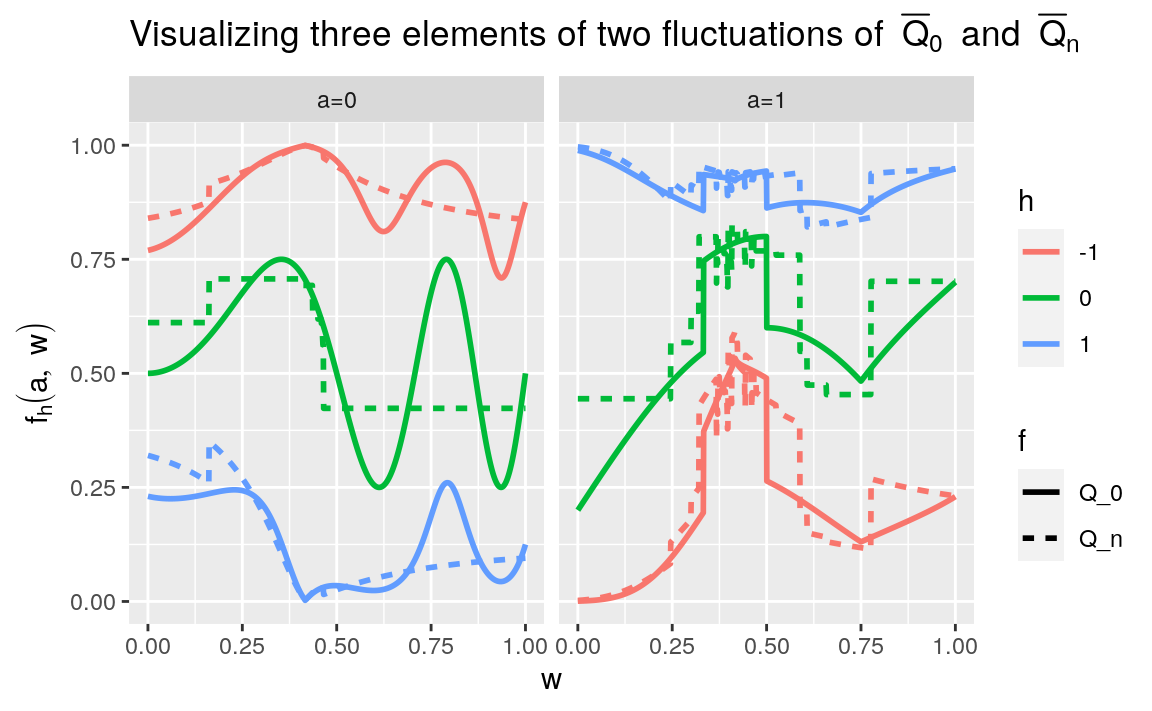
\includegraphics[width=0.7\linewidth]{img/fluctuation-1} 

}

\caption{Representing three elements \(\Qbar_{h}\) of the fluctuations \(\calQ(\Qbar_{0}, \Gbar_{0})\) and \(\calQ(\Qbar_{n,\text{trees}}, \Gbar_{0})\), respectively, where \(\Qbar_{n,\text{trees}}\) is an estimator of \(\Qbar_{0}\) derived by the boosted trees algorithm (see Section \ref{boosted-trees}). The three elements correspond to \(h=-1,0,1\). When \(h=0\), \(\Qbar_{h}\) equals either \(\Qbar_{0}\) or \(\Qbar_{n,\text{trees}}\), depending on which fluctuation is roamed.}\label{fig:fluctuation}
\end{figure}

\hypertarget{exo-fluct}{%
\subsection{\texorpdfstring{⚙ \gear More on fluctuations}{⚙ More on fluctuations}}\label{exo-fluct}}

\begin{enumerate}
\def\labelenumi{\arabic{enumi}.}
\item
  Justify the series of equalities in \eqref{eq:Qbarh}.
\item
  Justify that, in fact, if \(s(O)\) depends on \(O\) only through \((A,W)\) then
  the conditional law of \(Y\) given \((A,W)\) under \(P_{h}\) equals that under
  \(P\).
\end{enumerate}

\hypertarget{roaming}{%
\subsection{Targeted roaming of a fluctuation}\label{roaming}}

Recall that our goal is to build an estimator of \(\Qbar_0\) that is \emph{at least
as good} as \(\Qbar_n\). We will look for this enhanced estimator in the
fluctuation \(\calQ(\Qbar_{n}, \Gbar_{n})\) where \(\Gbar_{n}\) is an estimator of
\(\Gbar_{0}\) that is bounded away from 0 and 1. Thus, the estimator writes as
\(\Qbar_{n,h_{n}}\) for some data-driven \(h_{n} \in \bbR\). We will clarify why
we do so \protect\hyperlink{fluct-justification}{at a later time}

To assess the performance of all the candidates included in the fluctuation,
we formally rely on the empirical risk function \(h \mapsto \Exp_{P_{n}} \left(L_{y} (\Qbar_{n,h})(O)\right)\) where \begin{equation*}\Exp_{P_{n}}
\left(L_{y}   (\Qbar_{n,h})(O)\right)  =   \frac{1}{n}  \sum_{i=1}^{n}   L_{y}
(\Qbar_{n,h})(O_{i})\end{equation*} and the logistic (or negative binomial)
loss function \(L_{y}\) is given by
\begin{equation*} 
-L_{y}(f)(O) \defq Y
\log f(A,W) + (1 - Y) \log \left(1 - f(A,W)\right) \label{eq:logis-loss-y}
\end{equation*}
for any function \(f:\{0,1\} \times [0,1] \to [0,1]\). This loss
function is the counterpart of the loss function \(L_{a}\) defined in
\eqref{eq:logis-loss}. The justification that we gave in Section
\ref{logis-loss} of the relevance of \(L_{a}\) also applies here, \emph{mutatis
mutandis}. In summary, the oracle risk \(\Exp_{P_{0}} \left(L_{y} (f)(O)\right)\) of \(f\) is a real-valued measure of discrepancy between
\(\Qbar_{0}\) and \(f\); \(\Qbar_{0}\) minimizes \(f \mapsto \Exp_{P_{0}} \left(L_{y} (f)(O)\right)\) over the set of all (measurable) functions \(f:[0,1] \times \{0,1\} \times [0,1] \to [0,1]\); and a minimizer \(h_{0} \in \bbR\) of \(h \mapsto \Exp_{P_{0}} \left(L_{y} (\Qbar_{n,h})(O)\right)\) identifies the
element of fluctuation \(\calQ(\Qbar_{n}, \Gbar_{n})\) that is closest to
\(\Qbar_{0}\) (some details are given \protect\hyperlink{oracle-logistic-risk}{there} in Appendix
\ref{oracle-logistic-risk}).

It should not come as a surprise after this discussion that the aforementioned
data-driven \(h_{n}\) is chosen to be the minimizer of the empirical risk
function, \emph{i.e.}, \begin{equation*}h_{n} \defq  \mathop{\arg\min}_{h \in
\bbR}  \Exp_{P_{n}}  \left(L_{y}  (\Qbar_{n,h})(O)\right).\end{equation*} The
criterion is convex so the optimization program is well-posed.

The next chunk of code illustrates the search of an approximation of \(h_{n}\)
over a grid of candidate values.

\begin{Shaded}
\begin{Highlighting}[]
\NormalTok{candidates }\OtherTok{\textless{}{-}} \FunctionTok{seq}\NormalTok{(}\SpecialCharTok{{-}}\FloatTok{0.01}\NormalTok{, }\FloatTok{0.01}\NormalTok{, }\AttributeTok{length.out =} \FloatTok{1e4}\NormalTok{)}
\NormalTok{W }\OtherTok{\textless{}{-}}\NormalTok{ obs[}\DecValTok{1}\SpecialCharTok{:}\FloatTok{1e3}\NormalTok{, }\StringTok{"W"}\NormalTok{]}
\NormalTok{A }\OtherTok{\textless{}{-}}\NormalTok{ obs[}\DecValTok{1}\SpecialCharTok{:}\FloatTok{1e3}\NormalTok{, }\StringTok{"A"}\NormalTok{]}
\NormalTok{Y }\OtherTok{\textless{}{-}}\NormalTok{ obs[}\DecValTok{1}\SpecialCharTok{:}\FloatTok{1e3}\NormalTok{, }\StringTok{"Y"}\NormalTok{]}
\NormalTok{lGAW }\OtherTok{\textless{}{-}} \FunctionTok{compute\_lGbar\_hatAW}\NormalTok{(A, W, Gbar\_hat)}
\NormalTok{QAW }\OtherTok{\textless{}{-}} \FunctionTok{compute\_Qbar\_hatAW}\NormalTok{(A, W, Qbar\_hat\_trees)}
\NormalTok{risk }\OtherTok{\textless{}{-}} \FunctionTok{sapply}\NormalTok{(candidates,}
               \ControlFlowTok{function}\NormalTok{(h) \{}
\NormalTok{                 QAW\_h }\OtherTok{\textless{}{-}} \FunctionTok{expit}\NormalTok{(}\FunctionTok{logit}\NormalTok{(QAW)  }\SpecialCharTok{+}\NormalTok{ h }\SpecialCharTok{*}\NormalTok{ (}\DecValTok{2} \SpecialCharTok{*}\NormalTok{ A }\SpecialCharTok{{-}} \DecValTok{1}\NormalTok{) }\SpecialCharTok{/}\NormalTok{ lGAW)}
                 \SpecialCharTok{{-}}\FunctionTok{mean}\NormalTok{(Y }\SpecialCharTok{*} \FunctionTok{log}\NormalTok{(QAW\_h) }\SpecialCharTok{+}\NormalTok{ (}\DecValTok{1} \SpecialCharTok{{-}}\NormalTok{ Y) }\SpecialCharTok{*} \FunctionTok{log}\NormalTok{(}\DecValTok{1} \SpecialCharTok{{-}}\NormalTok{ QAW\_h))}
\NormalTok{               \})}
\NormalTok{idx\_min }\OtherTok{\textless{}{-}} \FunctionTok{which.min}\NormalTok{(risk)}
\NormalTok{idx\_zero }\OtherTok{\textless{}{-}} \FunctionTok{which.min}\NormalTok{(}\FunctionTok{abs}\NormalTok{(candidates))[}\DecValTok{1}\NormalTok{]}
\NormalTok{labels }\OtherTok{\textless{}{-}} \FunctionTok{c}\NormalTok{(}\FunctionTok{expression}\NormalTok{(R[n](}\FunctionTok{bar}\NormalTok{(Q)[}\FunctionTok{list}\NormalTok{(n,hn)]}\SpecialCharTok{\^{}}\FunctionTok{list}\NormalTok{(o))),}
            \FunctionTok{expression}\NormalTok{(R[n](}\FunctionTok{bar}\NormalTok{(Q)[}\FunctionTok{list}\NormalTok{(n,}\DecValTok{0}\NormalTok{)]}\SpecialCharTok{\^{}}\FunctionTok{list}\NormalTok{(o))))}
\NormalTok{risk }\SpecialCharTok{\%\textgreater{}\%}\NormalTok{ enframe }\SpecialCharTok{\%\textgreater{}\%}
  \FunctionTok{mutate}\NormalTok{(}\AttributeTok{h =}\NormalTok{ candidates) }\SpecialCharTok{\%\textgreater{}\%}
  \FunctionTok{filter}\NormalTok{(}\FunctionTok{abs}\NormalTok{(h }\SpecialCharTok{{-}}\NormalTok{ h[idx\_min]) }\SpecialCharTok{\textless{}=} \FunctionTok{abs}\NormalTok{(h[idx\_min])) }\SpecialCharTok{\%\textgreater{}\%}
  \FunctionTok{ggplot}\NormalTok{() }\SpecialCharTok{+}
  \FunctionTok{geom\_point}\NormalTok{(}\FunctionTok{aes}\NormalTok{(}\AttributeTok{x =}\NormalTok{ h, }\AttributeTok{y =}\NormalTok{ value), }\AttributeTok{color =} \StringTok{"\#CC6666"}\NormalTok{) }\SpecialCharTok{+}
  \FunctionTok{geom\_vline}\NormalTok{(}\AttributeTok{xintercept =} \FunctionTok{c}\NormalTok{(}\DecValTok{0}\NormalTok{, candidates[idx\_min])) }\SpecialCharTok{+}
  \FunctionTok{geom\_hline}\NormalTok{(}\AttributeTok{yintercept =} \FunctionTok{c}\NormalTok{(risk[idx\_min], risk[idx\_zero])) }\SpecialCharTok{+}
  \FunctionTok{scale\_y\_continuous}\NormalTok{(}
    \FunctionTok{bquote}\NormalTok{(}\StringTok{"empirical logistic risk, "} \SpecialCharTok{\textasciitilde{}}\NormalTok{ R[n](}\FunctionTok{bar}\NormalTok{(Q)[}\FunctionTok{list}\NormalTok{(n,h)]}\SpecialCharTok{\^{}}\FunctionTok{list}\NormalTok{(o))),}
    \AttributeTok{trans =} \StringTok{"exp"}\NormalTok{, }\AttributeTok{labels =} \ConstantTok{NULL}\NormalTok{, }
    \AttributeTok{sec.axis =} \FunctionTok{sec\_axis}\NormalTok{(}\SpecialCharTok{\textasciitilde{}}\NormalTok{ .,}
                        \AttributeTok{breaks =} \FunctionTok{c}\NormalTok{(risk[idx\_min], risk[idx\_zero]),}
                        \AttributeTok{labels =}\NormalTok{ labels))}
\end{Highlighting}
\end{Shaded}

\begin{figure}

{\centering 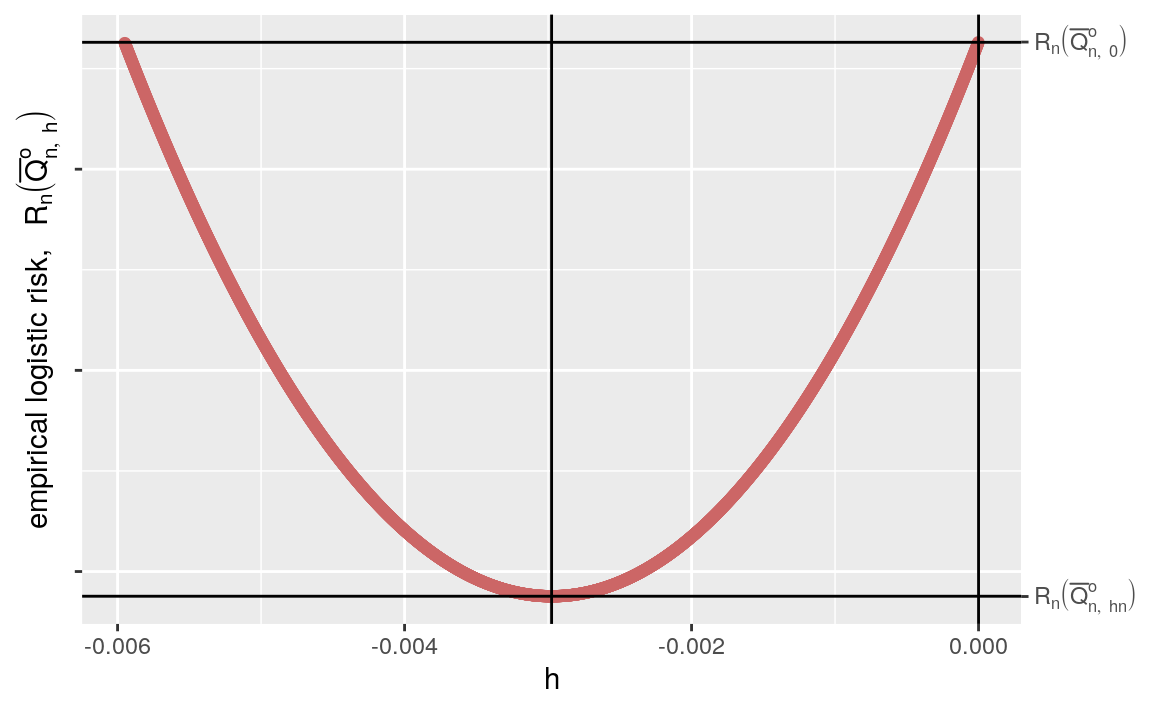
\includegraphics[width=0.7\linewidth]{img/grid-search-1} 

}

\caption{Representing the evolution of the empirical risk function as \(h\) ranges over a grid of values. One sees that the risk at \(h=0\) (\emph{i.e.}, the risk of \(\Qbar_{n}\)) is larger that the minimal risk, achieved at \(h \approx\) -0.003 (which must be close to that of the optimal \(\Qbar_{n,h_{n}}\)).}\label{fig:grid-search}
\end{figure}



Figure \ref{fig:grid-search} reveals how moving away slightly from \(h=0\) to
the left (\emph{i.e.}, to \(h_{n}\) equal to -0.003,
rounded to three decimal places) entails a decrease of the empirical risk. The
gain is modest at the scale of the empirical risk, but considerable in terms
of inference, as we explain below.

\hypertarget{fluct-justification}{%
\subsection{Justifying the form of the fluctutation}\label{fluct-justification}}

Let us define \(\Qbar_{n}^{*} \defq \Qbar_{n, h_{n}}\). We justify in two
steps our assertion that moving from \(\left.\Qbar_{n}\right|_{h=0} = \Qbar_{n}\) to \(\Qbar_{n}^{*}\) along fluctuation \(\calQ(\Qbar_{n}, \Gbar_{n})\)
has a considerable impact for the inference of \(\psi_{0}\).

First, we note that there is no need to iterate the updating procedure.
Specifically, even if we tried to fluctuate \(\Qbar_{n}^{*}\) along the
fluctuation \(\calQ(\Qbar_{n}^{*}, \Gbar_{n}) = \{\Qbar_{n,h'}^{*} : h' \in \bbR\}\) defined like \(\calQ(\Qbar_{n}, \Gbar_{n})\) \eqref{eq:Q-fluct} with
\(\Qbar_{n,h_{n}}\) substituted for \(\Qbar_{n}\), then we would not move at all.
This is obvious because there is a one-to-one smooth correspondence between
the parameter \(h'\) indexing \(\calQ(\Qbar_{n}^{*}, \Gbar_{n})\) and the
parameter \(h\) indexing \(\calQ(\Qbar_{n}, \Gbar_{n})\) (namely, \(h' = h + h_{n}\)). Therefore, the derivative of (the real-valued function over \(\bbR\))
\(h \mapsto \Exp_{P_n} \left(L_{y} (\Qbar_{n,h})(O)\right)\) evaluated at its
minimizer \(h_{n}\) equals 0. Equivalently (see \protect\hyperlink{fluct-score}{there} in
Appendix \ref{fluct-score} for a justification of the last but one equality
below),

\begin{align}\notag     \frac{d}{d      h}     &      \left.      \Exp_{P_{n}}
\left(L_{y}(\Qbar_{n,h}^{*})(O)\right)\right|_{h=0}      \\     \notag      &=
-\frac{1}{n}\left.\frac{d}{d     h}     \sum_{i=1}^{n}    \left(Y_{i}     \log
\Qbar_{n,h}^{*}(A_{i},    W_{i})    +    (1    -    Y_{i})    \log\left(1    -
\Qbar_{n,h}^{*}(A_{i}, W_{i})\right)\right)\right|_{h=0} \\ \notag &= -\frac{1}{n}\sum_{i=1}^{n} \left(\frac{Y_{i}}{\Qbar_{n}^{*}(A_{i}, W_{i})} - \frac{1 - Y_{i}}{1 - \Qbar_{n}^{*}(A_{i}, W_{i})}\right) \times \left.\frac{d}{d h} \Qbar_{n,h}^{*}(A_{i}, W_{i})\right|_{h=0} \\ \notag&= -\frac{1}{n}\sum_{i=1}^{n} \frac{Y_{i} - \Qbar_{n}^{*}(A_{i}, W_{i})}{\Qbar_{n}^{*}(A_{i}, W_{i}) \times \left(1 - \Qbar_{n}^{*}(A_{i}, W_{i})\right)} \left.\frac{d}{d h} \Qbar_{n,h}^{*}(A_{i}, W_{i})\right|_{h=0}  \\ &= -\frac{1}{n}\sum_{i=1}^{n} \frac{2A_{i} - 1}{\ell\Gbar_{n}(A_{i}, W_{i})} \left(Y_{i} - \Qbar_{n}^{*}(A_{i}, W_{i})\right) = 0. \label{eq:fluct-score}\end{align}

Second, let \(P_{n}^{*}\) be a law in \(\calM\) such that the \(Q_{W}\), \(\Gbar\) and
\(\Qbar\) features of \(P_{n}^{*}\) equal \(Q_{n,W}\), \(\Gbar_{n}\) and \(Q_{n}^{*}\),
respectively. In other words, \(P_{n}^{*}\) is compatible with \(Q_{n,W}\),
\(\Gbar_{n}\) and \(\Qbar_{n}^{*}\).\footnote{In Section \ref{analysis-of-plug-in}, we
  defined \(\Phat_{n}\) similarly with \(\Qbar_{n}\) substituted for
  \(\Qbar_{n}^{*}\).} Note that the last equality in \eqref{eq:fluct-score}
equivalently writes as \begin{equation*}P_{n}  D_{2}^{*}   (P_{n}^{*})  =
0.\end{equation*} Thus the (direct) fluctuation solves
\eqref{eq:solve-alt}. Now, we have already argued in Section \ref{basic-fact}
that it also holds that \begin{equation*}P_{n}  D_{1}^{*}  (P_{n}^{*})  =
0.\end{equation*} Consequently, \(P_{n}^{*}\) solves the efficient influence
curve equation, that is, satisfies \eqref{eq:solve}. As argued in Section
\ref{eic-equation}, it thus follows that the plug-in estimator
\begin{equation*}     \psi_n^*    \defq     \Psi(P_{n}^{*})    =     \int
\left(\Qbar_n^*(1,w)  - \Qbar_n^*(0,w)\right)  dQ_{n,W}(w) \end{equation*} is
asymptotically linear with influence curve \(\IC = D^{*}(P_{0})\), under mild
conditions. Moreover, by virtue of its plug-in construction, it has the
additional property that in finite-samples \(\psi_n^*\) will always obey bounds
on the parameter space.

\hypertarget{exo-tmle-flucs}{%
\subsection{\texorpdfstring{⚙ \gear Alternative fluctuation}{⚙ Alternative fluctuation}}\label{exo-tmle-flucs}}

The following exercises will have you consider an alternative means of
performing a fluctuation. For \(a = 0, 1\), consider the following
fluctuation model for \(\Qbar^a \defq \Qbar(a,\cdot)\):
\begin{equation} 
\calQ^a(\Qbar^a)
\defq      \left\{w       \mapsto      \Qbar_{h}^a(w)      \defq
\expit\left(\logit\left(\Qbar(a,w)\right) +  h
\right) : h \in \bbR\right\} \subset \calQ. \label{eq:Q-fluct-alt} 
\end{equation}
Let
\begin{equation*}
  \calQ^{\text{alt}}(\Qbar)   \defq   \left\{(a,w)  \mapsto   \Qbar_{h_0,
  h_1}(a,w) \defq a \times
  \Qbar_{h_{1}}^1(w) + (1-a) \Qbar_{h_{0}}^0(w) : h_{0}, h_{1} \in \bbR\right\}
\end{equation*}
be the fluctuation model for \(\Qbar\) that is implied by the two submodels for
\(\Qbar^1\) and \(\Qbar^0\).

Also for a given \(\Gbar\) satisfying that \(0 < \ell\Gbar(A,W) < 1\),
\(P_{0}\)-almost surely, and both \(a=0,1\), consider the loss function
\(L_{y,\Gbar}^{a}\) given by
\begin{equation*}
   L_{y,\Gbar}^{a} (f) (A,W) \defq\frac{\one\{A = a\}}{\ell\Gbar(A, W)} L_{y}
   (f)(O)
\end{equation*}
for any function \(f:\{0,1\} \times [0,1] \to [0,1]\), where \(L_{y}\) is defined
in \eqref{eq:logis-loss-y} above. It yields the
empirical risk function
\begin{equation*}
(h_{0}, h_{1}) \mapsto \sum_{a = 0,1}  \Exp_{P_{n}}
\left(L^a_{y, \Gbar} (\Qbar^a_{n,h_a})(O)\right).
\end{equation*}

\begin{enumerate}
\def\labelenumi{\arabic{enumi}.}
\item
  Comment on the differences between these fluctuation model and loss
  function compared to those discussed above.
\item
  Visualize three elements of \(\calQ^{\text{alt}}(\Qbar_0)\) and
  \(\calQ^{\text{alt}}(\Qbar_n)\): choose three values for \((h_0, h_1)\) and
  reproduce Figure \ref{fig:fluctuation}.
\item
  Argue that in order to minimize the empirical risk over all \((h_0, h_1) \in \bbR^2\), we may minimize over \(h_0 \in \bbR\) and \(h_1 \in \bbR\) separately.
\item
  Visualize how the empirical risk with \(\Gbar = \Gbar_n\) varies for different elements
  \(\Qbar_{n, h_0, h_1}\) of \(\calQ(\Qbar_n)\). For simplicity (and with the justification of problem 3),
  you may wish to make a separate figure (like Figure \ref{fig:grid-search}) for \(a = 0, 1\)
  that illustrates how the empirical risk varies as a function of \(h_a\) while setting \(h_{1 - a} = 0\).
\item
  ☡ \stixdanger{} Justify the validity of \(L^a_{y, \Gbar}\) as a loss function for \(\Qbar^a_0\):
  show that amongst all functions that map \(w\) to \((0,1)\), the true risk
  \(\Exp_{P_0}\left(L^a_{y, \Gbar}(f)(O)\right)\) is minimized when \(f = \Qbar^a_0\).
\item
  ☡ \stixdanger{} Argue that your answer to problem 2 also implies that the summed loss function \(\sum_{a=0,1} L^a_{y, \Gbar}\)
  is valid for \(\Qbar\).
\item
  ☡ \stixdanger{} Justify the combination of these loss function and fluctuation by repeating
  the calculation in equation \eqref{eq:fluct-score} above, \emph{mutatis mutandis}.
\end{enumerate}

\hypertarget{summary-and-perspectives}{%
\section{Summary and perspectives}\label{summary-and-perspectives}}

The procedure laid out in Section \ref{TMLE} is called \emph{targeted minimum
loss-based estimation} (TMLE). The nomenclature derives from its logistics.
We first generated an (un-targeted) initial estimator of \(\Psi(P_0)\) by
substituting for \(P_{0}\) a law \(\Phat_{n}\) compatible with initial estimators
of some \(\Psi\)-specific relevant nuisance parameters. Then through
loss-minimization, we built a \emph{targeted} estimator by substituting for
\(\Phat_{n}\) a law \(P_{n}^{*}\) compatible with the nuisance parameters that we
updated in a targeted fashion.

The TMLE procedure was coined in 2006 by Mark van der Laan and Dan Rubin
\citep{TMLE06}. It has since then been developed and applied in a great variety of
contexts. We refer to the monographies \citep{TMLEbook11} and \citep{TMLEbook18} for a
rich overview.

In summary, targeted learning bridges the gap between formal inference of
finite-dimensional parameters \(\Psi(P_{0})\) of the law \(P_{0}\) of the data,
via bootstrapping or influence curves, and data-adaptive, loss-based, machine
learning estimation of \(\Psi\)-specific infinite-dimensional features thereof
(the so-called nuisance parameters). A typical example concerns the super
learning-based, targeted estimation of effect parameters defined as
identifiable versions of causal quantities. The TMLE algorithm integrates
completely the estimation of the relevant nuisance parameters by super
learning \citep{SL07}. Under mild assumptions, the targeting step removes the bias
of the initial estimators of the targeted effects. The resulting TMLEs enjoy
many desirable statistical properties: among others, by being substitution
estimators, they lie in the parameter space; they are often double-robust;
they lend themselves to the construction of confidence regions.

The scientific community is always engaged in devising and promoting enhanced
principles for sounder research through the better design of experimental and
nonexperimental studies and the development of more reliable and honest
statistical analyses. By focusing on prespecified analytic plans and
algorithms that make realistic assumptions in more flexible nonparametric or
semiparametric statistical models, targeted learning has been at the forefront of
this concerted effort. Under this light, targeted learning notably consists in
translating knowledge about the data and underlying data-generating mechanism
into a realistic model; in expressing the research question under the form of
a statistical estimation problem; in analyzing the statistical estimation
problem within the frame of the model; in developing \emph{ad hoc} algorithms
grounded in theory and tailored to the question at stake to map knowledge and
data into an answer coupled to an assessment of its trustworthiness.

Quoting \citep{TMLEbook18}:

\begin{quote}
Over the last decade, targeted learning has been established as a reliable framework for constructing effect estimators and prediction functions. The continued development of targeted learning has led to new solutions for existing problems in many data structures in addition to discoveries in varied applied areas. This has included work in randomized controlled trials, parameters defined by a marginal structural model, case-control studies, collaborative TMLE, missing and censored data, longitudinal data, effect modification, comparative effectiveness research, aging, cancer, occupational exposures, plan payment risk adjustment, and HIV, as well as others. In many cases, these studies compared targeted learning techniques to standard approaches, demonstrating improved performance in simulations and realworld applications.
\end{quote}

It is now time to resume our introduction to TMLE and to carry out an
empirical investigation of its statistical properties in the context of the
estimation of \(\psi_{0}\).

\hypertarget{empirical-inves-tmle}{%
\section{Empirical investigation}\label{empirical-inves-tmle}}

\hypertarget{empirical-inves-tmle-first}{%
\subsection{A first numerical application}\label{empirical-inves-tmle-first}}

Let us illustrate the principle of targeted minimum loss estimation by
updating the G-computation estimator built on the \(n=1000\) first observations
in \texttt{obs} by relying on \(\Algo_{\Qbar,\text{kNN}}\), that is, on the algorithm
for the estimation of \(\Qbar_{0}\) as it is implemented in \texttt{estimate\_Qbar} with
its argument \texttt{algorithm} set to the built-in \texttt{kknn\_algo} (see Section
\ref{Qbar-knn-algo}). In Section \ref{empirical-inves-one-step}, we
performed a one-step correction of the same initial estimator.

The algorithm has been trained earlier on this data set and produced the
object \texttt{Qbar\_hat\_kknn}. The following chunk of code prints the initial
estimator \texttt{psin\_kknn}, its one-step update \texttt{psin\_kknn\_os}, then applies the
targeting step and presents the resulting estimator:

\begin{Shaded}
\begin{Highlighting}[]
\NormalTok{(psin\_kknn)}
\CommentTok{\#\textgreater{} \# A tibble: 1 x 2}
\CommentTok{\#\textgreater{}   psi\_n   sig\_n}
\CommentTok{\#\textgreater{}   \textless{}dbl\textgreater{}   \textless{}dbl\textgreater{}}
\CommentTok{\#\textgreater{} 1 0.101 0.00306}
\NormalTok{(psin\_kknn\_os)}
\CommentTok{\#\textgreater{} \# A tibble: 1 x 3}
\CommentTok{\#\textgreater{}    psi\_n  sig\_n    crit\_n}
\CommentTok{\#\textgreater{}    \textless{}dbl\textgreater{}  \textless{}dbl\textgreater{}     \textless{}dbl\textgreater{}}
\CommentTok{\#\textgreater{} 1 0.0999 0.0171 {-}0.000633}
\NormalTok{(psin\_kknn\_tmle }\OtherTok{\textless{}{-}} \FunctionTok{apply\_targeting\_step}\NormalTok{(}\FunctionTok{head}\NormalTok{(obs, }\FloatTok{1e3}\NormalTok{),}
                                        \FunctionTok{wrapper}\NormalTok{(Gbar\_hat, }\ConstantTok{FALSE}\NormalTok{),}
                                        \FunctionTok{wrapper}\NormalTok{(Qbar\_hat\_kknn, }\ConstantTok{FALSE}\NormalTok{)))}
\CommentTok{\#\textgreater{} \# A tibble: 1 x 3}
\CommentTok{\#\textgreater{}    psi\_n  sig\_n    crit\_n}
\CommentTok{\#\textgreater{}    \textless{}dbl\textgreater{}  \textless{}dbl\textgreater{}     \textless{}dbl\textgreater{}}
\CommentTok{\#\textgreater{} 1 0.0999 0.0171 {-}2.05e{-}17}
\end{Highlighting}
\end{Shaded}

In the call to \texttt{apply\_targeting\_step} we provide \emph{(i)} the data set at hand
(first line), \emph{(ii)} the estimator \texttt{Gbar\_hat} of \(\Gbar_{0}\) that we built
earlier by using algorithm \(\Algo_{\Gbar,1}\) (second line; see Section
\ref{algo-Gbar-one}), \emph{(iii)} the estimator \texttt{Qbar\_hat\_kknn} of \(\Qbar_{0}\)
(third line). Apparently, in this particular example, the one-step correction
and targeted correction updater similarly the initial estimator.

\hypertarget{exo-tmle}{%
\subsection{\texorpdfstring{⚙ \gear A computational exploration}{⚙ A computational exploration}}\label{exo-tmle}}

\begin{enumerate}
\def\labelenumi{\arabic{enumi}.}
\item
  Consult the man page of function \texttt{apply\_targeting\_step} (run
  \texttt{?apply\_targeting\_step}) and explain what is the role of its input
  \texttt{epsilon}.
\item
  Run the chunk of code below. What does it do? Hint: check out the chunks of
  code of Sections \ref{Qbar-knn-algo}, \ref{unknown-gbar-constr} and
  \ref{empirical-inves-tmle-first}.
\end{enumerate}



\begin{Shaded}
\begin{Highlighting}[]
\NormalTok{epsilon }\OtherTok{\textless{}{-}} \FunctionTok{seq}\NormalTok{(}\SpecialCharTok{{-}}\FloatTok{1e{-}2}\NormalTok{, }\FloatTok{1e{-}2}\NormalTok{, }\AttributeTok{length.out =} \FloatTok{1e2}\NormalTok{)}
\NormalTok{Gbar\_hat\_w }\OtherTok{\textless{}{-}} \FunctionTok{wrapper}\NormalTok{(Gbar\_hat, }\ConstantTok{FALSE}\NormalTok{)}
\NormalTok{Qbar\_kknn }\OtherTok{\textless{}{-}} \FunctionTok{wrapper}\NormalTok{(Qbar\_hat\_kknn, }\ConstantTok{FALSE}\NormalTok{)}

\NormalTok{psi\_trees\_epsilon }\OtherTok{\textless{}{-}} \FunctionTok{sapply}\NormalTok{(epsilon, }\ControlFlowTok{function}\NormalTok{(h) \{}
  \FunctionTok{apply\_targeting\_step}\NormalTok{(}\FunctionTok{head}\NormalTok{(obs, }\FloatTok{1e3}\NormalTok{), Gbar\_hat\_w,}
\NormalTok{                       Qbar\_trees, }\AttributeTok{epsilon =}\NormalTok{ h) }\SpecialCharTok{\%\textgreater{}\%}
    \FunctionTok{select}\NormalTok{(psi\_n, crit\_n) }\SpecialCharTok{\%\textgreater{}\%}\NormalTok{ as.matrix}
\NormalTok{\})}
\NormalTok{idx\_trees }\OtherTok{\textless{}{-}} \FunctionTok{which.min}\NormalTok{(}\FunctionTok{abs}\NormalTok{(psi\_trees\_epsilon[}\DecValTok{2}\NormalTok{, ]))}

\NormalTok{psi\_kknn\_epsilon }\OtherTok{\textless{}{-}} \FunctionTok{sapply}\NormalTok{(epsilon, }\ControlFlowTok{function}\NormalTok{(h) \{}
  \FunctionTok{apply\_targeting\_step}\NormalTok{(}\FunctionTok{head}\NormalTok{(obs, }\FloatTok{1e3}\NormalTok{), Gbar\_hat\_w,}
\NormalTok{                       Qbar\_kknn, }\AttributeTok{epsilon =}\NormalTok{ h) }\SpecialCharTok{\%\textgreater{}\%}
    \FunctionTok{select}\NormalTok{(psi\_n, crit\_n) }\SpecialCharTok{\%\textgreater{}\%}\NormalTok{ as.matrix}
\NormalTok{\})}
\NormalTok{idx\_kknn }\OtherTok{\textless{}{-}} \FunctionTok{which.min}\NormalTok{(}\FunctionTok{abs}\NormalTok{(psi\_kknn\_epsilon[}\DecValTok{2}\NormalTok{, ]))}

\FunctionTok{rbind}\NormalTok{(}\FunctionTok{t}\NormalTok{(psi\_trees\_epsilon), }\FunctionTok{t}\NormalTok{(psi\_kknn\_epsilon)) }\SpecialCharTok{\%\textgreater{}\%}\NormalTok{ as\_tibble }\SpecialCharTok{\%\textgreater{}\%}
  \FunctionTok{rename}\NormalTok{(}\StringTok{"psi\_n"} \OtherTok{=}\NormalTok{ V1, }\StringTok{"crit\_n"} \OtherTok{=}\NormalTok{ V2) }\SpecialCharTok{\%\textgreater{}\%}
  \FunctionTok{mutate}\NormalTok{(}\AttributeTok{type =} \FunctionTok{rep}\NormalTok{(}\FunctionTok{c}\NormalTok{(}\StringTok{"trees"}\NormalTok{, }\StringTok{"kknn"}\NormalTok{), }\AttributeTok{each =} \FunctionTok{length}\NormalTok{(epsilon))) }\SpecialCharTok{\%\textgreater{}\%} 
  \FunctionTok{ggplot}\NormalTok{() }\SpecialCharTok{+}
  \FunctionTok{geom\_point}\NormalTok{(}\FunctionTok{aes}\NormalTok{(}\AttributeTok{x =}\NormalTok{ crit\_n, }\AttributeTok{y =}\NormalTok{ psi\_n, }\AttributeTok{color =}\NormalTok{ type)) }\SpecialCharTok{+}
  \FunctionTok{geom\_vline}\NormalTok{(}\AttributeTok{xintercept =} \DecValTok{0}\NormalTok{) }\SpecialCharTok{+}
  \FunctionTok{geom\_hline}\NormalTok{(}\AttributeTok{yintercept =} \FunctionTok{c}\NormalTok{(psi\_trees\_epsilon[}\DecValTok{1}\NormalTok{,idx\_trees],}
\NormalTok{                            psi\_kknn\_epsilon[}\DecValTok{1}\NormalTok{,idx\_kknn])) }\SpecialCharTok{+}
  \FunctionTok{labs}\NormalTok{(}\AttributeTok{x =} \FunctionTok{bquote}\NormalTok{(}\FunctionTok{paste}\NormalTok{(P[n]}\SpecialCharTok{\textasciitilde{}}\NormalTok{D}\SpecialCharTok{\^{}}\StringTok{"*"}\NormalTok{, (P[}\FunctionTok{list}\NormalTok{(n,h)]}\SpecialCharTok{\^{}}\NormalTok{o))),}
       \AttributeTok{y =} \FunctionTok{bquote}\NormalTok{(}\FunctionTok{Psi}\NormalTok{(P[}\FunctionTok{list}\NormalTok{(n,h)]}\SpecialCharTok{\^{}}\NormalTok{o)))}
\end{Highlighting}
\end{Shaded}

\begin{figure}

{\centering 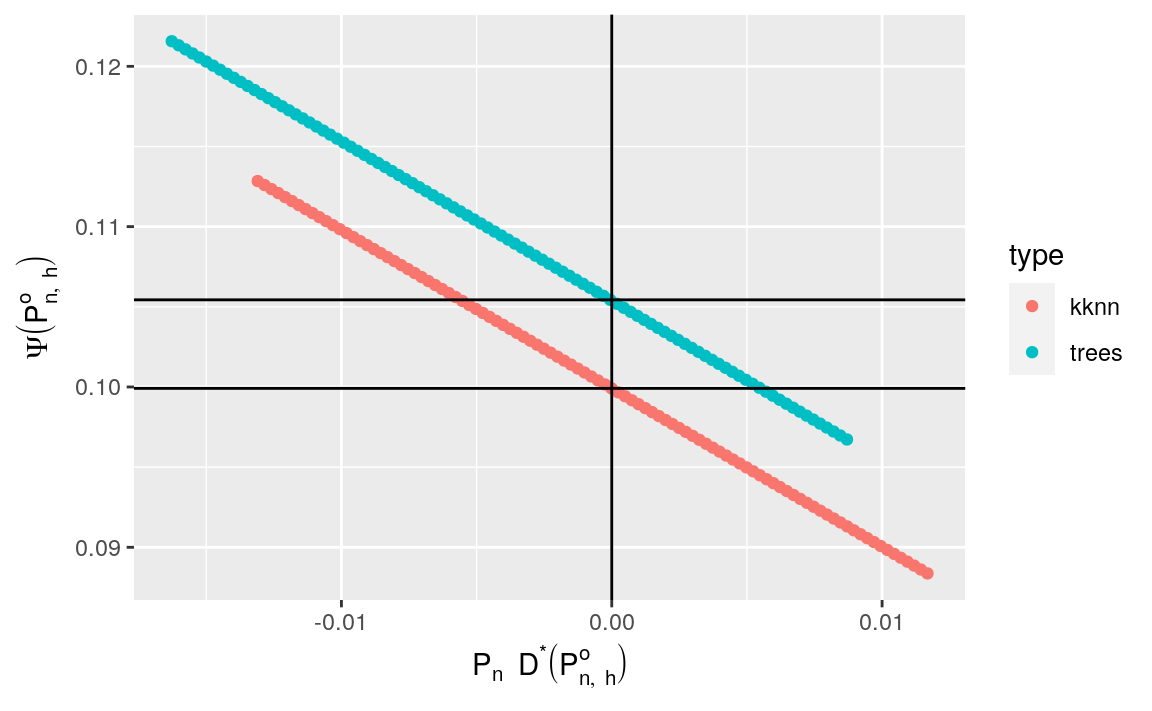
\includegraphics[width=0.7\linewidth]{img/exo-tmle-1} 

}

\caption{Figure produced when running the chunk of code from problem 2 in Section \ref{exo-tmle}.}\label{fig:exo-tmle}
\end{figure}

\begin{enumerate}
\def\labelenumi{\arabic{enumi}.}
\setcounter{enumi}{2}
\tightlist
\item
  Discuss the fact that the colored curves in Figure \ref{fig:exo-tmle}
  look like segments.
\end{enumerate}

\hypertarget{empirical-investigation}{%
\subsection{Empirical investigation}\label{empirical-investigation}}

To assess more broadly what is the impact of the targeting step, let us apply
it to the estimators that we built in Section \ref{empirical-inves-Gcomp}. In
Section \ref{empirical-inves-one-step}, we applied the one-step correction to
the same estimators.

The object \texttt{learned\_features\_fixed\_sample\_size} already contains the estimated
features of \(P_{0}\) that are needed to perform the targeting step on the
estimators \(\psi_{n}^{d}\) and \(\psi_{n}^{e}\), thus we merely have to call the
function \texttt{apply\_targeting\_step}.



\begin{Shaded}
\begin{Highlighting}[]
\NormalTok{psi\_tmle }\OtherTok{\textless{}{-}}\NormalTok{ learned\_features\_fixed\_sample\_size }\SpecialCharTok{\%\textgreater{}\%}
  \FunctionTok{mutate}\NormalTok{(}\AttributeTok{tmle\_d =}
           \FunctionTok{pmap}\NormalTok{(}\FunctionTok{list}\NormalTok{(obs, Gbar\_hat, Qbar\_hat\_d),}
                \SpecialCharTok{\textasciitilde{}} \FunctionTok{apply\_targeting\_step}\NormalTok{(}\FunctionTok{as.matrix}\NormalTok{(..}\DecValTok{1}\NormalTok{),}
                                 \FunctionTok{wrapper}\NormalTok{(..}\DecValTok{2}\NormalTok{, }\ConstantTok{FALSE}\NormalTok{),}
                                 \FunctionTok{wrapper}\NormalTok{(..}\DecValTok{3}\NormalTok{, }\ConstantTok{FALSE}\NormalTok{))),}
         \AttributeTok{tmle\_e =}
           \FunctionTok{pmap}\NormalTok{(}\FunctionTok{list}\NormalTok{(obs, Gbar\_hat, Qbar\_hat\_e),}
                \SpecialCharTok{\textasciitilde{}} \FunctionTok{apply\_targeting\_step}\NormalTok{(}\FunctionTok{as.matrix}\NormalTok{(..}\DecValTok{1}\NormalTok{),}
                                 \FunctionTok{wrapper}\NormalTok{(..}\DecValTok{2}\NormalTok{, }\ConstantTok{FALSE}\NormalTok{),}
                                 \FunctionTok{wrapper}\NormalTok{(..}\DecValTok{3}\NormalTok{, }\ConstantTok{FALSE}\NormalTok{)))) }\SpecialCharTok{\%\textgreater{}\%}
  \FunctionTok{select}\NormalTok{(tmle\_d, tmle\_e) }\SpecialCharTok{\%\textgreater{}\%}
  \FunctionTok{pivot\_longer}\NormalTok{(}\FunctionTok{c}\NormalTok{(}\StringTok{\textasciigrave{}}\AttributeTok{tmle\_d}\StringTok{\textasciigrave{}}\NormalTok{, }\StringTok{\textasciigrave{}}\AttributeTok{tmle\_e}\StringTok{\textasciigrave{}}\NormalTok{),}
               \AttributeTok{names\_to =} \StringTok{"type"}\NormalTok{, }\AttributeTok{values\_to =} \StringTok{"estimates"}\NormalTok{) }\SpecialCharTok{\%\textgreater{}\%}
  \FunctionTok{extract}\NormalTok{(type, }\StringTok{"type"}\NormalTok{, }\StringTok{"\_([de])$"}\NormalTok{) }\SpecialCharTok{\%\textgreater{}\%}
  \FunctionTok{mutate}\NormalTok{(}\AttributeTok{type =} \FunctionTok{paste0}\NormalTok{(type, }\StringTok{"\_targeted"}\NormalTok{)) }\SpecialCharTok{\%\textgreater{}\%}
  \FunctionTok{unnest}\NormalTok{(estimates) }\SpecialCharTok{\%\textgreater{}\%}
  \FunctionTok{group\_by}\NormalTok{(type) }\SpecialCharTok{\%\textgreater{}\%}
  \FunctionTok{mutate}\NormalTok{(}\AttributeTok{sig\_alt =} \FunctionTok{sd}\NormalTok{(psi\_n)) }\SpecialCharTok{\%\textgreater{}\%}
  \FunctionTok{mutate}\NormalTok{(}\AttributeTok{clt\_ =}\NormalTok{ (psi\_n }\SpecialCharTok{{-}}\NormalTok{ psi\_zero) }\SpecialCharTok{/}\NormalTok{ sig\_n,}
         \AttributeTok{clt\_alt =}\NormalTok{ (psi\_n }\SpecialCharTok{{-}}\NormalTok{ psi\_zero) }\SpecialCharTok{/}\NormalTok{ sig\_alt) }\SpecialCharTok{\%\textgreater{}\%}
  \FunctionTok{pivot\_longer}\NormalTok{(}\FunctionTok{c}\NormalTok{(}\StringTok{\textasciigrave{}}\AttributeTok{clt\_}\StringTok{\textasciigrave{}}\NormalTok{, }\StringTok{\textasciigrave{}}\AttributeTok{clt\_alt}\StringTok{\textasciigrave{}}\NormalTok{),}
               \AttributeTok{names\_to =} \StringTok{"key"}\NormalTok{, }\AttributeTok{values\_to =} \StringTok{"clt"}\NormalTok{) }\SpecialCharTok{\%\textgreater{}\%}
  \FunctionTok{extract}\NormalTok{(key, }\StringTok{"key"}\NormalTok{, }\StringTok{"\_(.*)$"}\NormalTok{) }\SpecialCharTok{\%\textgreater{}\%}
  \FunctionTok{mutate}\NormalTok{(}\AttributeTok{key =} \FunctionTok{ifelse}\NormalTok{(key }\SpecialCharTok{==} \StringTok{""}\NormalTok{, }\ConstantTok{TRUE}\NormalTok{, }\ConstantTok{FALSE}\NormalTok{)) }\SpecialCharTok{\%\textgreater{}\%}
  \FunctionTok{rename}\NormalTok{(}\StringTok{"auto\_renormalization"} \OtherTok{=}\NormalTok{ key)}

\NormalTok{(bias\_tmle }\OtherTok{\textless{}{-}}\NormalTok{ psi\_tmle }\SpecialCharTok{\%\textgreater{}\%}
   \FunctionTok{group\_by}\NormalTok{(type, auto\_renormalization) }\SpecialCharTok{\%\textgreater{}\%}
   \FunctionTok{summarize}\NormalTok{(}\AttributeTok{bias =} \FunctionTok{mean}\NormalTok{(clt)) }\SpecialCharTok{\%\textgreater{}\%}\NormalTok{ ungroup)}
\CommentTok{\#\textgreater{} \# A tibble: 4 x 3}
\CommentTok{\#\textgreater{}   type       auto\_renormalization     bias}
\CommentTok{\#\textgreater{}   \textless{}chr\textgreater{}      \textless{}lgl\textgreater{}                   \textless{}dbl\textgreater{}}
\CommentTok{\#\textgreater{} 1 d\_targeted FALSE                {-}0.0147 }
\CommentTok{\#\textgreater{} 2 d\_targeted TRUE                 {-}0.0313 }
\CommentTok{\#\textgreater{} 3 e\_targeted FALSE                 0.0132 }
\CommentTok{\#\textgreater{} 4 e\_targeted TRUE                 {-}0.00407}

\NormalTok{fig }\OtherTok{\textless{}{-}} \FunctionTok{ggplot}\NormalTok{() }\SpecialCharTok{+}
  \FunctionTok{geom\_line}\NormalTok{(}\FunctionTok{aes}\NormalTok{(}\AttributeTok{x =}\NormalTok{ x, }\AttributeTok{y =}\NormalTok{ y), }
            \AttributeTok{data =} \FunctionTok{tibble}\NormalTok{(}\AttributeTok{x =} \FunctionTok{seq}\NormalTok{(}\SpecialCharTok{{-}}\DecValTok{4}\NormalTok{, }\DecValTok{4}\NormalTok{, }\AttributeTok{length.out =} \FloatTok{1e3}\NormalTok{),}
                          \AttributeTok{y =} \FunctionTok{dnorm}\NormalTok{(x)),}
            \AttributeTok{linetype =} \DecValTok{1}\NormalTok{, }\AttributeTok{alpha =} \FloatTok{0.5}\NormalTok{) }\SpecialCharTok{+}
  \FunctionTok{geom\_density}\NormalTok{(}\FunctionTok{aes}\NormalTok{(clt, }\AttributeTok{fill =}\NormalTok{ type, }\AttributeTok{colour =}\NormalTok{ type),}
\NormalTok{               psi\_tmle, }\AttributeTok{alpha =} \FloatTok{0.1}\NormalTok{) }\SpecialCharTok{+}
  \FunctionTok{geom\_vline}\NormalTok{(}\FunctionTok{aes}\NormalTok{(}\AttributeTok{xintercept =}\NormalTok{ bias, }\AttributeTok{colour =}\NormalTok{ type),}
\NormalTok{             bias\_tmle, }\AttributeTok{size =} \FloatTok{1.5}\NormalTok{, }\AttributeTok{alpha =} \FloatTok{0.5}\NormalTok{) }\SpecialCharTok{+}
  \FunctionTok{facet\_wrap}\NormalTok{(}\SpecialCharTok{\textasciitilde{}}\NormalTok{ auto\_renormalization,}
             \AttributeTok{labeller =}
               \FunctionTok{as\_labeller}\NormalTok{(}\FunctionTok{c}\NormalTok{(}\StringTok{\textasciigrave{}}\AttributeTok{TRUE}\StringTok{\textasciigrave{}} \OtherTok{=} \StringTok{"auto{-}renormalization: TRUE"}\NormalTok{,}
                             \StringTok{\textasciigrave{}}\AttributeTok{FALSE}\StringTok{\textasciigrave{}} \OtherTok{=} \StringTok{"auto{-}renormalization: FALSE"}\NormalTok{)),}
             \AttributeTok{scales =} \StringTok{"free"}\NormalTok{)}
  
\NormalTok{fig }\SpecialCharTok{+}
  \FunctionTok{labs}\NormalTok{(}\AttributeTok{y =} \StringTok{""}\NormalTok{,}
       \AttributeTok{x =} \FunctionTok{bquote}\NormalTok{(}\FunctionTok{paste}\NormalTok{(}\FunctionTok{sqrt}\NormalTok{(n}\SpecialCharTok{/}\NormalTok{v[n]}\SpecialCharTok{\^{}}\NormalTok{\{}\StringTok{"*"}\NormalTok{\})}\SpecialCharTok{*}
\NormalTok{                        (psi[n]}\SpecialCharTok{\^{}}\NormalTok{\{}\StringTok{"*"}\NormalTok{\} }\SpecialCharTok{{-}}\NormalTok{ psi[}\DecValTok{0}\NormalTok{]))))}
\end{Highlighting}
\end{Shaded}

\begin{figure}

{\centering 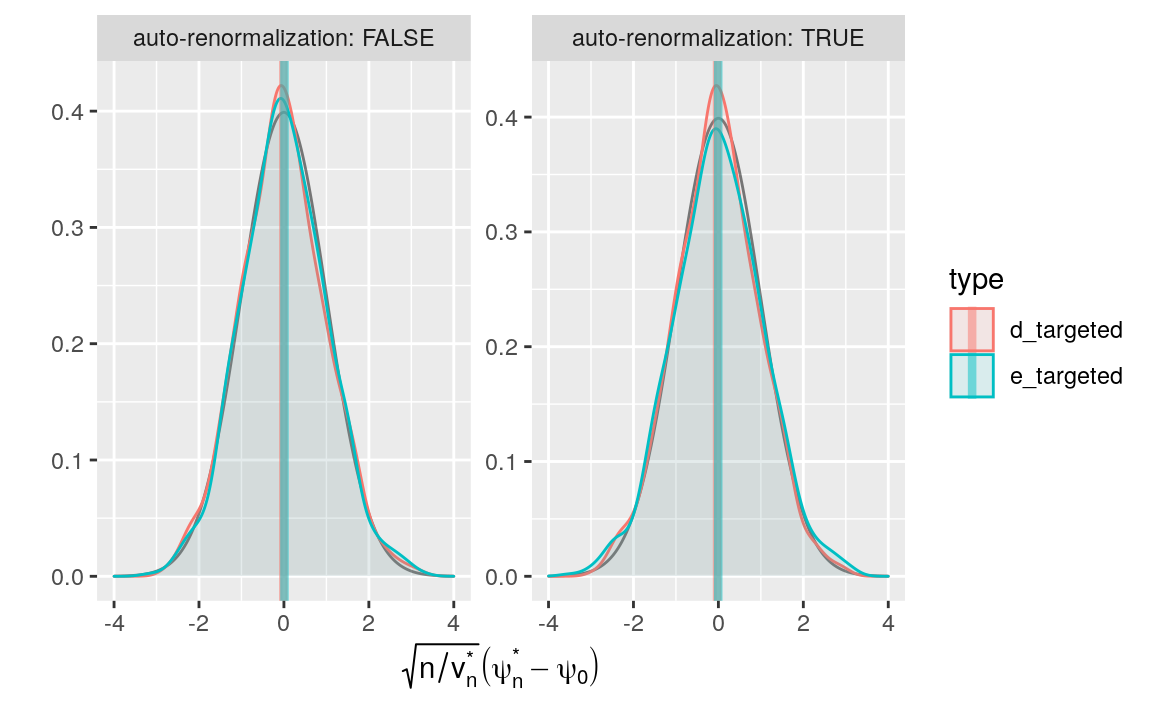
\includegraphics[width=0.7\linewidth]{img/tmle-1} 

}

\caption{Kernel density estimators of the law of two targeted estimators of \(\psi_{0}\) (recentered with respect to \(\psi_{0}\), and renormalized). The estimators respectively hinge on algorithms \(\Algo_{\Qbar,1}\) (d) and \(\Algo_{\Qbar,\text{kNN}}\) (e) to estimate \(\Qbar_{0}\), and on a targeting step. Two renormalization schemes are considered, either based on an estimator of the asymptotic variance (left) or on the empirical variance computed across the 1000 independent replications of the estimators (right). We emphasize that the \(x\)-axis ranges differ between the left and right plots.}\label{fig:tmle}
\end{figure}

We see that the step of targeting is as promised: the bias of the resulting
estimators is minimized relative to the naive estimators. Comparing
these results to those obtain using one-step estimators (Section
\ref{empirical-inves-one-step}), we find quite similar performance between
one-step and TMLE estimators.

\hypertarget{closing-words}{%
\chapter{Closing words}\label{closing-words}}

The velocity of advances in machine learning make it an exciting time to work as
a statistician. Clearly, statistical inference is more challenging when one
considers the sort of infinite-dimensional statistical models that underlie
these developments. Even defining some fundamental statistical notions, like
efficiency, in these settings is a challenge. Constructing estimators that
obtain these properties is more challenging still. We hope that this short guide
has provided an approachable introduction to this exciting area of research.

Targeted learning is a vibrant and active field of research, with new
developments happening along theoretical, applied, and computational axes. The
\href{https://tlverse.org/}{\texttt{tlverse}} software environment is actively being
developed to provide researchers with new tools for utilizing these methods.

\hypertarget{appendix-appendix}{%
\appendix}


\hypertarget{notation}{%
\chapter{Notation}\label{notation}}

\begin{itemize}
\item
  \(\defq\), equal by definition to
\item
  \(\one\{S\}\), the indicator of statement \(S\), which equals 1 if \(S\) is true
  and 0 otherwise.
\item
  \(O \defq (W,A,Y)\), the generic summary of how one realization of the experiments
  of interest unfold, our generic observation; \(W \in [0,1]\) is the context of
  action, \(A \in \{0,1\}\) is the action undertaken, and \(Y\in [0,1]\) is the
  reward of action \(A\) in context \(W\). We denote by \(\calO \defq [0,1] \times \{0,1\} \times [0,1]\) the set where a generic \(O\) takes its values.
\item
  \(P\), \(P_{0}\), \(\Pi_{0}\), \(\Pi_{h}\), \(\Pi_{0}'\), \(\Pi_{h}'\), laws (on \(\calO\))
  for \(O\).
\item
  \(Pf \defq \Exp_{P} (f(O))\) for any law \(P\) for \(O\) and function \(f\) from
  \(\calO\) to \(\bbR^{p}\).
\item
  \(\|f\|_{P}^{2} \defq Pf^{2} = \Exp_{P} (f(O)^{2}) = \int f(o)^{2} dP(o)\),
  the square of the \(L^{2}(P)\)-norm of \(f\), a function from \(\calO\) to \(\bbR\).
\item
  \(\|f\|_{\infty} \defq \sup_{o \in \calO} |f(o)|\), the essential supremum of
  \(f\), a function from \(\calO\) to \(\bbR\).
\item
  \(P_{n}\), the empirical measure. If the observations are \(O_{1}\), \ldots,
  \(O_{n}\), then \(P_{n}\) is a law such that the generic random variable \(O\) drawn
  from \(P_{n}\) takes its values in \(\{O_{1}, \ldots, O_{n}\}\) in such a way that
  \(O = O_{i}\) with probability \(n^{-1}\) for each \(1 \leq i \leq n\).
\item
  \(\sqrt{n} (P_{n} - P)\), where \(P_{n}\) is the empirical measure associated to
  \(O_{1}, \ldots, O_{n}\) drawn independently from \(P\), the empirical process.
\item
  \(X_n = o_{P_0}(1)\) if \(X_n\), a random variable built from \(O_{1}\), \ldots,
  \(O_{n}\) independently drawn from \(P_0\), converges in probability to zero, that
  is, if \(P_0(|X_n| > t)\) converges to zero for all \(t>0\) as \(n\) goes to
  infinity. If \(n^{c} X_n = o_{P_0}(1)\), then one also writes \(X_n = o_{P_0}(n^{-c})\).
\item
  \(X_{n} = O_{P_0}(1)\) if \(X_n\), a random variable built from \(O_{1}\), \ldots,
  \(O_{n}\) independently drawn from \(P_0\), is bounded in probability, that
  is if, for all \(t>0\) there exists \(M >0\) such that \(\sup_{n \geq 1} P_0(|X_n| \geq M) \leq t\). If \(n^{c} X_n = O_{P_0}(1)\), then one also writes \(X_n = O_{P_0}(n^{-c})\).
\item
  \(\calM\), the model, that is, the collection of \emph{all} laws from which \(O\)
  can be drawn and that meet some constraints.
\item
  \(\calM^{\text{empirical}}\), the collection of all discrete laws on \([0,1] \times \{0,1\} \times [0,1]\), of which \(P_{n}\) is a distinguished element.
\item
  \(Q_{W}\), \(Q_{0,W}\), marginal laws for \(W\) (under \(P\) and \(P_{0}\),
  respectively).
\item
  \(\Gbar(W) \defq \Pr_{P}(A = 1 | W)\), \(\Gbar_0(W) \defq \Pr_{P_0}(A = 1 | W)\), conditional probabilities of action \(A = 1\) given \(W\) (under \(P\) and
  \(P_{0}\), respectively). For each \(a \in \{0,1\}\), \(\ell\Gbar(a,W) \defq \Pr_{P}(A = a | W)\) and \(\ell\Gbar_0(a,W) \defq \Pr_{P_0}(A = a | W)\).
\item
  \(\Qbar(A,W) = \Exp_{P}(Y|A,W)\), \(\Qbar_0(A,W) = \Exp_{P_{0}}(Y|A,W)\), the
  conditional means of \(Y\) given \(A\) and \(W\) (under \(P\) and \(P_{0}\),
  respectively).
\item
  \(\calQ \defq \{\Qbar : P \in \calM\}\), the space of regression
  functions induced by model \(\calM\).
\item
  \(\calQ(\Qbar,\Gbar) \subset \calQ\), \(\Gbar\)-specific fluctuation model of
  \(\Qbar\), see \eqref{eq:Q-fluct}.
\item
  \(q_{Y}\), \(q_{0,Y}\), conditional densities of \(Y\) given \(A\) and \(W\) (under
  \(P\) and \(P_{0}\), respectively).
\item
  \(\Psi : \calM \to [0,1]\), given by \(\Psi(P) \defq \int \left(\Qbar(1, w) - \Qbar(0, w)\right)dQ_{W}(w)\), the statistical mapping of interest.
\item
  \(\psi \defq \Psi(P)\), \(\psi_{0} \defq \Psi(P_{0})\).
\item
  \(\Algo\), \(\Algo_{\Gbar,1}\), \(\Algo_{\Qbar,1}\), algorithms to be trained on
  \(P_{n}\), \emph{i.e.}, mappings from \(\calM^{\text{empirical}}\) to the set where
  lives the feature targeted by the algorithm.
\item
  \(\Algora_{\Gbar,s}\), \(\Algora_{\Qbar,s}\), \(s\)-specific oracle algorithms
  (\(s>0\)) that can use the true targeted features \(\Gbar_{0}\) and \(\Qbar_{0}\)
  to produce predictions that are almost exact, up to a \(N(0,s^{2})\) random
  error term.
\item
  \(L_{a}\), the contex-specific logistic (or negative binomial) loss function,
  given by \(-L_{a}(f)(A,W) \defq A \log f(W) + (1-A) \log (1-f(W))\) for
  any function \(f:[0,1]\to[0,1]\).
\item
  \(L_{y}\), the reward-specific logistic (or negative binomial) loss function,
  given by \(-L_{y}(f)(O) \defq Y \log f(A,W) + (1-Y) \log (1-f(A,W))\) for
  any function \(f:\{0,1\} \times [0,1] \to[0,1]\).
\end{itemize}

\hypertarget{proofs}{%
\chapter{Basic results and their proofs}\label{proofs}}

\hypertarget{npsem}{%
\section{NPSEM}\label{npsem}}

The experiment can also be summarized by a \emph{nonparametric system of structural
equations}: for some deterministic functions \(f_w\), \(f_a\), \(f_y\) and
independent sources of randomness \(U_w\), \(U_a\), \(U_y\),

\begin{enumerate}
\def\labelenumi{\arabic{enumi}.}
\item
  sample the context where the counterfactual rewards will be generated, the
  action will be undertaken and the actual reward will be obtained, \(W = f_{w}(U_w)\);
\item
  sample the two counterfactual rewards of the two actions that can be
  undertaken, \(Y_{0} = f_{y}(0, W, U_y)\) and \(Y_{1} = f_{y}(1, W, U_y)\);
\item
  sample which action is carried out in the given context, \(A = f_{a} (W, U_a)\);
\item
  define the corresponding reward, \(Y = A Y_{1} + (1-A) Y_{0}\);
\item
  summarize the course of the experiment with the observation \(O = (W, A, Y)\), thus concealing \(Y_{0}\) and \(Y_{1}\).
\end{enumerate}

\hypertarget{identification}{%
\section{Identification}\label{identification}}

Let \(\bbP_{0}\) be an experiment that generates \(\bbO \defq (W, Y_{0}, Y_{1}, A, Y)\). We think of \(W\) as the context where an action is undertaken, of
\(Y_{0}\) and \(Y_{1}\) as the counterfactual (potential) rewards that actions
\(a=0\) and \(a=1\) would entail, of \(A\) as the action carried out, and of \(Y\) as
the reward received in response to action \(A\). Consider the following
assumptions:

\begin{enumerate}
\def\labelenumi{\arabic{enumi}.}
\item
  \textbf{Randomization}: under \(\bbP_{0}\), the counterfactual rewards
  \(Y_0\), \(Y_1\) and action \(A\) are conditionally independent given \(W\), \emph{i.e.},
  \(Y_a \perp A \mid W\) for \(a=0,1\).
\item
  \textbf{Consistency}: under \(\bbP_{0}\), if action \(A\) is undertaken then reward
  \(Y_{A}\) is received, \emph{i.e.}, \(Y = Y_{A}\) (or \(Y=Y_{a}\) given that \(A=a\)).
\item
  \textbf{Positivity}: under \(\bbP_{0}\), both actions \(a=0\) and \(a=1\) have
  (\(\bbP_{0}\)-almost surely) a positive probability to be undertaken given
  \(W\), \emph{i.e.}, \(\Pr_{\bbP_0}(\ell\Gbar_0(a,W) > 0) = 1\) for \(a=0,1\).
\end{enumerate}

\begin{proposition}[Identification]
\protect\hypertarget{prp:unnamed-chunk-2}{}\label{prp:unnamed-chunk-2}Under the above assumptions, it holds that \begin{equation*}  \psi_{0}  =
\Exp_{\bbP_{0}}   \left(Y_{1}   -   Y_{0}\right)  =   \Exp_{\bbP_{0}}(Y_1)   -
\Exp_{\bbP_{0}}(Y_0). \end{equation*}
\end{proposition}

\begin{proof}
Set arbitrarily \(a \in \{0,1\}\). By the randomization assumption on the one
hand (second equality) and by the consistency and positivity assumptions on
the other hand (third equality), it holds that \begin{align*}
\Exp_{\bbP_0}(Y_a) &=  \int \Exp_{\bbP_0}(Y_a \mid  W = w) dQ_{0,W}(w)  = \int
\Exp_{\bbP_0}(Y_a \mid A = a, W =  w) dQ_{0,W}(w) \\ &= \int \Exp_{P_0}(Y \mid
A =  a, W = w)  dQ_{0,W}(w) = \int \Qbar_0(a,W)  dQ_{0,W}(w). \end{align*} The
stated result easily follows.
\end{proof}

\textbf{Remark.} The positivity assumption is needed for \(\Exp_{P_0}(Y \mid A = a, W) \defq \Qbar_{0}(a,W)\) to be well-defined.

\hypertarget{confidence-interval}{%
\section{Building a confidence interval}\label{confidence-interval}}

Let \(\Phi\) be the standard normal distribution function. Let \(X_{1}\),
\(\ldots\), \(X_{n}\) be independently drawn from a given law.

\hypertarget{clt}{%
\subsection{CLT \& Slutsky's lemma}\label{clt}}

Assume that \(\sigma^{2} \defq \Var(X_{1})\) is finite. Let \(m \defq \Exp(X_{1})\) be the mean of \(X_{1}\) and \(\bar{X}_{n} \defq n^{-1} \sum_{i=1}^{n} X_{i}\) be the empirical mean. By the central limit theorem
(CLT), it holds that \(\sqrt{n} (\bar{X}_{n} - m)\) converges in law as \(n\)
grows to the centered Gaussian law with variance \(\sigma^{2}\).

Moreover, if \(\sigma_{n}^{2}\) is a (positive) consistent estimator of
\(\sigma^{2}\) then, by Slutsky's lemma, \(\sqrt{n}/\sigma_{n} (\bar{X}_{n} - m)\)
converges in law to the standard normal law. The empirical variance \(n^{-1} \sum_{i=1}^{n}(X_{i} - \bar{X}_{n})^{2}\) is such an estimator.

\begin{proposition}
\protect\hypertarget{prp:unnamed-chunk-4}{}\label{prp:unnamed-chunk-4}Under the above assumptions, \begin{equation*}  \left[\bar{X}_{n}   \pm
\Phi^{-1}(1-\alpha)  \frac{\sigma_{n}}{\sqrt{n}}\right]  \end{equation*} is a
confidence interval for \(m\) with asymptotic level \((1-2\alpha)\).
\end{proposition}

\hypertarget{order}{%
\subsection{CLT and order statistics}\label{order}}

Suppose that the law of \(X_{1}\) admits a continuous distribution function
\(F\). Set \(p \in ]0,1[\) and, assuming that \(n\) is large, find \(k\geq 1\) and \(l \geq 1\) such that \begin{equation*}   \frac{k}{n}   \approx    p   -
\Phi^{-1}(1-\alpha)      \sqrt{\frac{p(1-p)}{n}}      \end{equation*} and
\begin{equation*}    \frac{l}{n}     \approx    p     +    \Phi^{-1}(1-\alpha)
\sqrt{\frac{p(1-p)}{n}}.  \end{equation*}

\begin{proposition}
\protect\hypertarget{prp:unnamed-chunk-5}{}\label{prp:unnamed-chunk-5}Under the above assumptions, \([X_{(k)},X_{(l)}]\) is a confidence interval for
\(F^{-1}(p)\) with asymptotic level \(1 - 2\alpha\).
\end{proposition}

\hypertarget{another-rep}{%
\section{Another representation of the parameter of interest}\label{another-rep}}

For notational simplicitiy, note that \((2a-1)\) equals 1 if \(a=1\) and \(-1\) if
\(a=0\). Now, for each \(a = 0,1\), \begin{align*}
\Exp_{P_{0}}\left(\frac{\one\{A    =    a\}Y}{\ell\Gbar_{0}(a,W)}\right)    &=
\Exp_{P_{0}}\left(\Exp_{P_{0}}\left(\frac{\one\{A  = a\}Y}{\ell\Gbar_{0}(a,W)}
\middle|  A,  W  \right)   \right)  \\  &=  \Exp_{P_{0}}\left(\frac{\one\{A  =
a\}}{\ell\Gbar_{0}(a,W)}      \Qbar_{0}(A,      W)     \right)      \\      &=
\Exp_{P_{0}}\left(\frac{\one\{A   =    a\}}{\ell\Gbar_{0}(a,W)}   \Qbar_{0}(a,
W)\right)    \\    &=   \Exp_{P_{0}}\left(\Exp_{P_{0}}\left(\frac{\one\{A    =
a\}}{\ell\Gbar_{0}(a,W)}  \Qbar_{0}(a, W)  \middle|  W \right)  \right) \\&  =
\Exp_{P_{0}}\left(\frac{\ell\Gbar_{0}(a,W)}{\ell\Gbar_{0}(a,W)}   \Qbar_{0}(a,
W)  \middle| W  \right) \\&  =  \Exp_{P_{0}} \left(  \Qbar_{0}(a, W)  \right),
\end{align*} where the first, fourth and sixth equalities follow from the
tower rule\footnote{For any random variable \((U,V)\) such that \(\Exp(U|V)\) and
  \(\Exp(U)\) are well defined, it holds that \(\Exp(\Exp(U|V)) = \Exp(U)\).}, and
the second and fifth hold by definition of the conditional expectation. This
completes the proof.

\hypertarget{prop-delta-method}{%
\section{The delta-method}\label{prop-delta-method}}

Let \(f\) be a map from \(\Theta \subset \bbR^{p}\) to \(\bbR^{q}\) that is
differentiable at \(\theta\in \Theta\). Let \(X_{n}\) be a random vector taking its
values in \(\Theta\).

\begin{proposition}
\protect\hypertarget{prp:unnamed-chunk-6}{}\label{prp:unnamed-chunk-6}If \(\sqrt{n} (X_{n} - \theta)\) converges in law to the Gaussian law with mean
\(\mu\) and covariance matrix \(\Sigma\), then \(\sqrt{n} (f(X_{n}) - f(\theta))\)
converge in law to the Gaussian law with mean \(\nabla f(\theta) \times \mu\)
and covariance matrix \(\nabla f(\theta) \times \Sigma \times \nabla f(\theta)^{\top}\). In addition, if \(\Sigma_{n}\) estimates \(\Sigma\)
consistently then, by Slutsky's lemma, the asymptotic variance of \(\sqrt{n} (f(X_{n}) - f(\theta))\) is consistently estimated with \(\nabla f(X_{n}) \times \Sigma_{n} \times \nabla f(X_{n})^{\top}\).
\end{proposition}

\hypertarget{oracle-logistic-risk}{%
\section{The oracle logistic risk}\label{oracle-logistic-risk}}

First, let us recall the definition of the Kullback-Leibler divergence between
Bernoulli laws of parameters \(p,q\in]0,1[\):
\begin{equation*}\text{KL}(p,q)  \defq  p \log\left(\frac{p}{q}\right)  +
(1-p) \log \left(\frac{1-p}{1-q}\right).\end{equation*}
It satisfies \(\text{KL}(p,q) \geq 0\) where the equality holds if and only if
\(p=q\).

Let \(f:[0,1] \times \{0,1\} \times [0,1] \to [0,1]\) be a (measurable)
function. Applying the tower rule shows that the oracle logistic risk
satisfies
\begin{align} 
\Exp_{P_{0}}  \left(L_{y}   (f)(O)\right)&=\Exp_{P_{0}}  \left(-\Qbar_{0}(A,W)
\log   f(A,W)   -   \left(1   -  \Qbar_{0}   (A,W)\right)   \log   \left(1   -
f(A,W)\right)\right)\notag\\&=\Exp_{P_{0}}
\left(\text{KL}\left(\Qbar_{0}(A,W),           f(A,W)\right)\right)          +
\text{constant},\label{eq:KL} 
\end{align}
where the above constant equals \begin{equation*} -\Exp_{P_{0}}\left(\Qbar_{0}(A,W) \log \Qbar_{0}(A,W) - \left(1 - \Qbar_{0} (A,W)\right) \log \left(1 - \Qbar_{0,W}(A,W)\right)\right).  \end{equation*}

In light of \eqref{eq:KL}, \(\Qbar_{0}\) minimizes \(f \mapsto \Exp_{P_{0}} \left(L_{y} (f)(O)\right)\) over the set of (measurable) functions mapping
\([0,1] \times \{0,1\} \times [0,1]\) to \([0,1]\). Moreover, as an average of
measures of discrepancy, \(\Exp_{P_{0}} \left(L_{y} (f)(O)\right)\) is also a
measure of discrepancy.

\hypertarget{more-proofs}{%
\chapter{More results and their proofs}\label{more-proofs}}

\hypertarget{estimation-of-the-asymptotic-variance-of-an-estimator}{%
\section{Estimation of the asymptotic variance of an estimator}\label{estimation-of-the-asymptotic-variance-of-an-estimator}}

\hypertarget{iptw-est-var}{%
\subsection{IPTW estimator based on a well-specified model}\label{iptw-est-var}}

\textbf{Sketch of proof.} The IPTW estimator \(\psi_{n}^{b}\) relies on algorithm
\(\Algo_{\Gbar,1}\), which is ``well-specified''\index{well/mis-specified} in the
sense that its output \(\Gbar_{n}\defq \Algo_{\Gbar,1}(P_{n})\) minimizes the
empirical risk over a finite-dimensional, identifiable, well-specified working
model for \(\Gbar_{0}\). If one introduces \(D\) given by

\begin{equation*}
D(O) \defq \frac{(2A-1)}{\ell\Gbar_{0}(A,W)} Y,
\end{equation*}

then the influence curve of \(\psi_{n}^{b}\) equals \(D - \Psi(P_{0})\) minus the
projection of \(D\) onto the tangent space of the above parametric model for
\(\Gbar_{0}\). The variance of the influence curve is thus smaller than that of
\(D\), hence the conservativeness.

\hypertarget{gcomp-est-var}{%
\subsection{G-computation estimator based on a well-specified model}\label{gcomp-est-var}}

\textbf{Sketch of proof} (see \citep{TMLEbook11} page 527). Consider a G-computation
estimator \(\psi_{n}\) that relies on an algorithm \(\Algo_{\Qbar}\) that is
``well-specified''\index{well/mis-specified} in the sense that its output
\(\Qbar_{n}\defq \Algo_{\Qbar}(P_{n})\) minimizes the empirical risk over a
finite-dimensional, identifiable, well-specified working model for
\(\Qbar_{0}\). If one introduces \(D\) given by

\begin{equation*}
D(O) \defq \Qbar_{0}(1,W) - \Qbar_{0}(0,W)
\end{equation*}

then the influence curve of \(\psi_{n}\) equals \(D - \Psi(P_{0})\) plus a
function of \(O\) that is orthogonal to \(D - \Psi(P_{0})\). Thus the variance of
the influence curve is larger than that of \(D\), hence the
anti-conservativeness.

\hypertarget{app-analysis-of-plug-in}{%
\section{\texorpdfstring{☡ \stixdanger{} General analysis of plug-in estimators}{☡  General analysis of plug-in estimators}}\label{app-analysis-of-plug-in}}

Recall that \(\Algo_{Q_{W}}\) is an algorithm designed for the estimation of
\(Q_{0,W}\) (see Section \ref{nuisance-QW}) and that we denote by \(Q_{n,W} \defq \Algo_{Q_{W}}(P_{n})\) the output of the algorithm trained on \(P_{n}\).
Likewise, \(\Algo_{\Gbar}\) and \(\Algo_{\Qbar}\) are two generic algorithms
designed for the estimation of \(\Gbar_{0}\) and of \(\Qbar_{0}\) (see Sections
\ref{nuisance-Gbar} and \ref{nuisance-Qbar}), \(\Gbar_{n} \defq \Algo_{\Gbar}(P_{n})\) and \(\Qbar_{n} \defq \Algo_{\Qbar}(P_{n})\) are their
outputs once trained on \(P_{n}\).

Let us now introduce \(\Phat_n\) a law in \(\calM\) such that the \(Q_{W}\), \(\Gbar\)
and \(\Qbar\) features of \(\Phat_n\) equal \(Q_{n,W}\), \(\Gbar_{n}\) and
\(\Qbar_{n}\), respectively. We say that any such law is \emph{compatible} with
\(Q_{n,W}\), \(\Gbar_n\) and \(\Qbar_n\).

\hypertarget{app-analysis-of-plug-in-main}{%
\subsection{Main analysis}\label{app-analysis-of-plug-in-main}}

Substituting \(\Phat_n\) for \(P\) in \eqref{eq:taylor-expansion} yields
\eqref{eq:hard-to-study}:
\begin{equation} 
\sqrt{n} (\Psi(\Phat_n) - \Psi(P_0)) =  - \sqrt{n} P_0 D^*(\Phat_n) + \sqrt{n}
\Rem_{P_0}(\Phat_n), 
\end{equation}

an equality that we rewrite as
\begin{align} 
\sqrt{n} (\Psi(\Phat_n) - \Psi(P_0)) = - & \sqrt{n} P_n D^*(\Phat_n) + \sqrt{n}
(P_n - P_0) D^*(P_0)\\ & + \sqrt{n}(P_n - P_0) [D^*(\Phat_n) - D^*(P_0)] +
\sqrt{n}\Rem_{P_0}(\Phat_n). 
\end{align}

Let us know study in turn the four terms in the above right-hand side
sum. Recall that \(X_n = o_{P_0}(1)\) means that \(P_0(|X_n| > t)\) converges to
zero for all \(t>0\) as \(n\) goes to infinity.

\begin{enumerate}
\def\labelenumi{\arabic{enumi}.}
\item
  In view of \eqref{eq:rem-two}, the fourth term is \(o_{P_0}(1)\) provided that
  \(\sqrt{n}\|\Qbar - \Qbar_{0}\|_{P_0} \times \|(\Gbar - \Gbar_{0})/\ell\Gbar_{0}\|_{P_0} = o_{P_0}(1)\). This is the case if, for
  instance, \(\ell\Gbar_{0}\) is bounded away from zero, and both
  \(n^{1/4}\|\Qbar - \Qbar_{0}\|_{P_0}\) and \(n^{1/4}\|\Gbar - \Gbar_{0}\|_{P_0}\) are \(o_{P_0}(1)\). What really matters, remarkably, is
  the \emph{product} of the two norms. If each norm goes to zero at rate
  \(n^{1/4}\), then their product does at rate \(\sqrt{n}\). Of course, if one
  goes to zero at rate \(n^{1/4 + c}\) for some \(0<c<1/4\), then it suffices
  that the other go to zero at rate \(n^{1/4 - c}\). See also Section
  \ref{asymp-neglig-remain}.
\item
  A fundamental result from empirical processes theory gives us conditions
  guaranteeing that the third term is \(o_{P_0}(1)\). By Lemma 19.24 in
  \citep{vdV98}, this is the case indeed if \(\|D^*(\Phat_n) - D^*(P_0)\|_{P_{0}} = o_{P_0} (1)\) (that is, if \(D^*(\Phat_n)\) estimates consistently \(D^*(P_0)\)) and if
  \(D^*(\Phat_n)\) falls (with probability tending to one) into a Donsker class
  (meaning that the random \(D^*(\Phat_n)\) must belong eventually to a set
  that is not too large). Requesting that \(\|D^*(\Phat_n) - D^*(P_0)\|_{P_{0}} = o_{P_0} (1)\) is not much if one is already willing to assume that
  \(n^{1/4}\|\Qbar - \Qbar_{0}\|_{P_0}\) and \(n^{1/4}\|\Gbar - \Gbar_{0}\|_{P_0}\) are \(o_{P_0}(1)\). Moreover, the second condition can be
  interpreted as a condition on the complexity/versatility of algorithms
  \(\Algo_{\Gbar}\) and \(\Algo_{\Qbar}\).
\item
  By the central limit theorem, the second term converges in law to the
  centered Gaussian law with variance \(P_0 D^*(P_0)^2\).
\item
  As for the first term, all we can say is that it is a potentially large
  (because of the \(\sqrt{n}\) renormalization factor) \emph{bias term}.
\end{enumerate}

\hypertarget{estimation-of-the-asymptotic-variance}{%
\subsection{Estimation of the asymptotic variance}\label{estimation-of-the-asymptotic-variance}}

Let us show now that, under the assumptions we made in Section
\ref{app-analysis-of-plug-in-main} and additional assumptions of similar
nature, \(P_{n} D^{*} (\Phat_n)^2\) estimates consistently the asymptotic
variance \(P_{0} D^{*} (P_{0})^2\). The proof hinges again on a decomposition
of the difference between the two quantities as a sum of three terms:
\begin{align}  P_{n} D^{*}  (\Phat_n)^2 -  P_{0} D^{*}  (P_{0})^2= &  (P_{n} -
P_{0}) \left(D^{*} (\Phat_n)^2 - D^{*}  (P_{0})^2\right)\\ & + (P_{n} - P_{0})
D^{*}  (P_{0})^2 +  P_{0}  (D^{*} \left(\Phat_n)^2  - D^{*}  (P_{0})^2\right).
\end{align}

We study the three terms in turn. Recall that \(X_n = o_{P_0}(1/\sqrt{n})\)
means that \(P_0(\sqrt{n}|X_n| > t)\) converges to zero for all \(t>0\) as \(n\)
goes to infinity.

\begin{enumerate}
\def\labelenumi{\arabic{enumi}.}
\item
  In light of the study of the third term in Section
  \ref{app-analysis-of-plug-in-main}, if \(\|D^*(\Phat_n)^2 - D^*(P_0)^2\|_{P_{0}} = o_{P_0} (1)\) and if \(D^*(\Phat_n)^{2}\) falls (with
  probability tending to one) into a Donsker class, then the first term is
  \(o_{P_0}(1/\sqrt{n})\). Furthermore, if \(D^*(\Phat_n)\) falls (with
  probability tending to one) into a Donsker class, an assumption we made
  earlier, then so does \(D^*(\Phat_n)^{2}\). In addition, if
  \(\|D^*(\Phat_n) - D^*(P_0)\|_{P_{0}} = o_{P_0} (1)\), another assumption we
  made earlier, and if there exists a constant \(c>0\) such that
  \begin{equation} \sup_{n \geq 1}  \|D^*(\Phat_n) + D^*(P_0)\|_{\infty} \leq
  c \label{eq:bounded-sup-norm}  \end{equation} \(P_{0}\)-almost surely, then \(\|D^*(\Phat_n)^2 - D^*(P_0)^2\|_{P_{0}} = o_{P_0} (1)\) too because \begin{equation}
  \|D^*(\Phat_n)^2   -   D^*(P_0)^2\|_{P_{0}}   \leq   c   \|D^*(\Phat_n)   -
  D^*(P_0)\|_{P_{0}}.  \end{equation} The existence of such a constant \(c\) is
  granted whenever \(\ell\Gbar_{0}\) and \(\ell\Gbar_{n}\) are bounded away from
  zero. Note that the condition on \(\ell\Gbar_{n}\) can be inforced by us
  through the specification of algorithm \(\Algo_{\Gbar}\).
\item
  By the central limit theorem, \(\sqrt{n}\) times the second term converges in
  law to the centered Gaussian law with variance \(\Var_{P_{0}} (D^{*} (P_{0})(O)^2)\), which is finite whenever \(\ell\Gbar_{0}\) is bounded away
  from zero. By Theorem 2.4 in \citep{vdV98}, the second term is thus \(O_{P_0} (1/\sqrt{n})\) hence \(o_{P_0} (1)\).
\item
  Finally, under assumption \eqref{eq:bounded-sup-norm}, the absolute value of
  the third term is smaller than \begin{equation}c  P_{0} |D^*(\Phat_n)  -
  D^*(P_0)|     \leq    c     \|D^*(\Phat_n)    -     D^*(P_0)\|_{P_{0}}    =
  o_{P_0}(1),\end{equation} where the inequality follows from the
  Cauchy-Schwarz inequality.
\end{enumerate}

In conclusion, \(P_{n} D^{*} (\Phat_n)^2 - P_{0} D^{*} (P_{0})^2 = o_{P_0}(1)\),
hence the result.

\hypertarget{asymp-neglig-remain}{%
\section{Asymptotic negligibility of the remainder term}\label{asymp-neglig-remain}}

Recall that \(\|f\|_{P}^{2} \defq \Exp_{P} \left( f(O)^{2} \right)\) is the
\(L_2(P)\)-norm of \(f\), a measurable function from \(\calO\) to \(\bbR\). Assume
that for \(a= 0,1\), \(\ell\Gbar_{n}(a,W) \geq \delta > 0\) \(Q_{0,W}\)-almost
everywhere.

The Cauchy-Schwarz inequality then implies that, for \(a = 0,1\),
\begin{equation*}\Rem_{P_0}(\Phat_n)   \le   \frac{2}{\delta}   \max_{a=0,1}
\left(  \|\Qbar_n   (a,\cdot)  -  \Qbar_0  (a,\cdot)\|_{P_0}   \right)  \times
\|\Gbar_n  -   \Gbar_0\|_{P_0}.\end{equation*} Therefore, if for \(a=0,1\),
\begin{equation*}\|\Qbar_n(a,\cdot)      -     \Qbar_0(a,\cdot)\|_{P_0}      =
o_{P_0}(n^{-1/4})\end{equation*} \emph{and} \begin{equation*}\|\Gbar_n     -
\Gbar_0\|_{P_0}        =         o_{P_0}(n^{-1/4}),\end{equation*} then
\begin{equation*}\Rem_{P_0}(\Phat_n) = o_{P_0}(n^{-1/2}).\end{equation*}

\hypertarget{analysis-TMLE}{%
\section{Analysis of targeted estimators}\label{analysis-TMLE}}

\hypertarget{basic-eic-eq}{%
\subsection{A basic fact on the influence curve equation}\label{basic-eic-eq}}

Recall the definition of \(D_{1}^{*}\) \eqref{eq:eif}. For \emph{any} estimator
\(\Qbar_n^*\) of \(\Qbar_0\) and a law \(P_n^{*}\) that is compatible with
\(\Qbar_n^*\) and \(Q_{n,W}\), it holds that
\begin{align*}
P_n D_1^*(P_n^*) 
&= \frac{1}{n} \sum_{i=1}^n D_1^{*}(P_n^*)(O_i)\\ 
&=\frac{1}{n}  \sum_{i=1}^n  \left(  \Qbar_n(1,W_i)   -  \Qbar_n(0,W_i)  -  \int
\left(\Qbar_n(1,w) - \Qbar_n(0,w)\right) dQ_{n,W}(w) \right) \\ 
&=   \frac{1}{n}\sum_{i=1}^n \left( \Qbar_n(1,W_i)  - \Qbar_n(0,W_i)\right) - \frac{1}{n}\sum_{i=1}^n
\left(\Qbar_n(1,W_i) - \Qbar_n(0,W_i)\right) = 0.
\end{align*}

\hypertarget{fluct-reg}{%
\subsection{Fluctuation of the regression function along the fluctuation of a law}\label{fluct-reg}}

Let us resume the discussion where we left it at the end of Section
\ref{smooth-second-pass-fluctuations}. Let \(\Qbar\) be the conditional mean
of \(Y\) given \((A,W)\) under \(P\). Set arbitrarily \(h \in H \setminus \{0\}\) and
a measurable function \((w,a) \mapsto f(a,w)\) taking non-negative
values. Applying repeatedly the tower rule yields the following equalities:
\begin{align*} \Exp_{P_{h}}  \left(f(A,W) Y\right) &= \Exp_{P}  \left(f(A,W) Y
(1 + h  s(O))\right) \\ &= \Exp_{P} \left(f(A,W) \Exp_{P}\left(Y  (1 + h s(O))
\middle|A,W\right)\right)  \\ &=  \Exp_{P} \left(f(A,W)  \left(\Qbar(A,W) +  h
\Exp_{P}(Ys(O)   |   A,W)   \right)\right)   \\   &=   \Exp_{P}   \left(f(A,W)
\frac{\Qbar(A,W) + h  \Exp_{P}(Ys(O) | A,W)}{1 +  h \Exp_{P}(s(O)|A,W)} \times
\left(1 + h \Exp_{P}(s(O)|A,W)\right)\right).\end{align*} Now, \eqref{eq:fluct}
implies that the density of \((A,W)\) under \(P_{h}\) equals \(\left(1 + h \Exp_{P}(s(O)|A,W)\right)\) when it is evaluated at \((A,W)\). Therefore, the
last inequality rewrites as
\begin{equation*} 
\Exp_{P_{h}}  \left(f(A,W)
Y\right)  = \Exp_{P_{h}}  \left(f(A,W) \frac{\Qbar(A,W)  + h  \Exp_{P}(Ys(O) |
A,W)}{1 + h \Exp_{P}(s(O)|A,W)}\right).
\end{equation*}
Since this equality is valid
for an arbitary \((w,a) \mapsto f(a,w)\) with non-negative values, we can deduce
from it that the conditional mean of \(Y\) given \((A,W)\) under \(P_h\) equals
\begin{equation*}\frac{\Qbar(A,W)   +  h   \Exp_{P}(Ys(O)   |   A,W)}{1  +   h
\Exp_{P}(s(O)|A,W)}.\end{equation*}

\hypertarget{fluct-score}{%
\subsection{Computing the score of a fluctuation of the regression function}\label{fluct-score}}

Let us resume the discussion where we left it at the beginning of Section
\ref{fluct-direct}. Set \(\alpha, \beta \in \bbR\). The derivative of \(h \mapsto \expit(\alpha + \beta h)\) evaluated at \(h=0\) satisfies
\begin{equation*}\frac{d}{dh}  \left.\expit(\alpha +  \beta h)\right|_{h=0}  =
\beta \expit(\alpha)  (1 - \expit(\alpha)).\end{equation*} Therefore, for any
\((w,a) \in [0,1] \times \{0,1\}\),
\begin{align*}\frac{d}{dh} \left.\Qbar_{h} (a, w)\right|_{h=0} &= \frac{2a - 1}{\ell\Gbar(a,w)} \expit\left(\logit\left(\Qbar(a,w)\right)\right) \left[1 - \expit\left(\logit\left(\Qbar(a,w)\right)\right)\right]\\&= \frac{2a - 1}{\ell\Gbar(a,w)} \Qbar(a,w) \left(1 - \Qbar(a,w)\right).\end{align*}
This justifies the last but one equality in \eqref{eq:fluct-score}.

Furthermore the same derivations that led to \eqref{eq:fluct-score} also imply,
\emph{mutatis mutandis}, that

\begin{equation*}  \frac{d}{d  h} \left.   L_{y}(\Qbar_{h})(O)\right|_{h=0}  =
\frac{2A      -      1}{\ell\Gbar(A,      W)}     \left(Y      -      \Qbar(A,
W)\right). \label{eq:fluct-score-bis}\end{equation*}

In this light, and in view of \eqref{eq:score}, we can think of \(\calQ(\Qbar, \Gbar)\) as a fluctuation of \(\Qbar\) in the direction of \begin{equation*}(w,a,y)     \mapsto    \frac{2a-1}{\ell\Gbar(a,w)}     (y     -
\Qbar(a,w)).\end{equation*} Thus if \(P \in \calM\) is such that
\(\Exp_{P}(Y|A,W) = \Qbar(A,W)\) and \(P(A=1|W) = \Gbar(W)\), then we can also
think of \(\calQ(\Qbar, \Gbar)\) as a fluctuation of \(\Qbar\) in the direction of
the second component \(D_{2}^{*}(P)\) of the efficient influence curve
\(D^{*}(P)\) of \(\Psi\) at \(P\) \eqref{eq:eif}.

  \bibliography{bibliography.bib}

\printindex
%%% Local Variables:
%%% mode: latex
%%% TeX-master: t
%%% End:

\end{document}
